%----------------------------------------------------------------------------------------
% PACKAGES AND OTHER DOCUMENT CONFIGURATIONS
%----------------------------------------------------------------------------------------

% !TEX encoding = UTF-8
% !TEX TS-program = pdflatex
% !TEX root = computabilità e algoritmi.tex
% !TEX spellcheck = it-IT

\documentclass[a4paper, 11pt]{report} % Font size (can be 10pt, 11pt or 12pt) and paper size (remove a4paper for US letter paper)
\usepackage[italian]{babel}      							% Lingua italiana
\usepackage[margin=.9in]{geometry}             % Imposta i margini del documento

\usepackage[T1]{fontenc} % Required for accented characters
\usepackage[mathletters]{ucs}    % Caratteri matematici come UTF8
\usepackage[utf8,utf8x]{inputenc}      % Ancora utf8

\usepackage{eurosym}                %simbolo dell'euro
\usepackage{listings}
\usepackage[usenames,dvipsnames,svgnames,table]{xcolor}
% Imposta lo spazio nella list of listing in modo simile alla list of figures/tables
%\makeatletter
%\let\my@chapter\@chapter
%\renewcommand*{\@chapter}{%
%  \addtocontents{lol}{\protect\addvspace{10pt}}%
%  \my@chapter}
%\makeatother


\definecolor{codegreen}{rgb}{0,0.6,0}
\definecolor{codegray}{rgb}{0.5,0.5,0.5}
\definecolor{backcolor}{rgb}{0.98,0.98,0.98}

\renewcommand{\lstlistingname}{Codice}% Listing -> codice
\renewcommand{\lstlistlistingname}{Elenco dei frammenti di codice}% List of Listings -> Frammenti di codice

\lstdefinestyle{mystyle}{
    backgroundcolor=\color{backcolor},   
    commentstyle=\color{Peach}\ttfamily,
    keywordstyle=\color{RoyalBlue},
    numberstyle=\tiny\color{codegray},
    stringstyle=\color{SeaGreen}\ttfamily,
    basicstyle=\footnotesize\ttfamily,
    breakatwhitespace=false,         
    breaklines=true,                 
    captionpos=b,                    
    keepspaces=true,                 
    numbers=left,                    
    numbersep=5pt,                  
    showspaces=false,                
    showstringspaces=false,
    showtabs=false,                  
    tabsize=2,
    frame=trbl, % draw a frame at the top, right, left and bottom of the listing
	frameround=ftff, % angolo in basso a destro curvo
	framesep=4pt, % quarter circle size of the round corners,
	inputencoding=utf8,
    extendedchars=true,
    literate={á}{{\'a}}1 {à}{{\`a}}1 {é}{{\'e}}1 {è}{{\`e}}1 {ù}{{\`u}}1 {ò}{{\`o}}1 {ì}{{\`i}}1,
    belowskip=1em,
    aboveskip=1em,
}

 
\lstset{style=mystyle}

\lstdefinelanguage{JavaScript}
{
  % list of keywords
  morekeywords={ true, false, catch, function, break,	new, class, extends, var, require, switch, return, import, if, while, for, this, View, Text, StyleSheet},
  sensitive=false, % keywords are not case-sensitive
  morecomment=[l]{//}, % l is for line comment
  morecomment=[s]{/*}{*/}, % s is for start and end delimiter
  morestring=[b]' % defines that strings are enclosed in double quotes
}

\lstdefinelanguage{JSON}
{
  % list of keywords
  morekeywords={string, boolean, int, Array, Node, Asset, AssetDetail, Filter, FilterItem},
  sensitive=false, % keywords are not case-sensitive
  morecomment=[l]{//}, % l is for line comment
  morecomment=[s]{/*}{*/}, % s is for start and end delimiter
  morestring=[b]" % defines that strings are enclosed in double quotes
}

\lstdefinelanguage{URM}
{
	% list of keywords
	morekeywords={ S, J, T, Z, I},
	sensitive=false, % keywords are not case-sensitive
	morecomment=[l]{//}, % l is for line comment
	morecomment=[s]{/*}{*/}, % s is for start and end delimiter
	morestring=[b]' % defines that strings are enclosed in double quotes
}

\lstdefinelanguage{RDFA}{
	language=html,
	sensitive=true, 
	alsoletter={<>=-},
	ndkeywords={
		% General
		=,
		% HTML attributes
		charset=, id=, width=, height=, property=, about=, rel=, rev=, prefix=, vocab=, content=, datatype=
	},  
	morecomment=[s]{<!--}{-->},
	tag=[s]
}

%\tightlist per compatibilità con pandoc
\providecommand{\tightlist}{%
  \setlength{\itemsep}{0pt}\setlength{\parskip}{0pt}}


\usepackage[labelfont=bf]{caption}

\usepackage[protrusion=true,expansion=true]{microtype} % Better typography
\usepackage{graphicx} % Required for including pictures
\usepackage{wrapfig} % Allows in-line images


\usepackage{subfig}
\usepackage{hyperref}
\usepackage{placeins}
\usepackage{sourcecodepro}
\usepackage{hyperref}                   % collegamenti ipertestuali

\usepackage[colorinlistoftodos,prependcaption]{todonotes} %todo

\usepackage{amsmath}
\usepackage{mathtools}

\usepackage{float}
\usepackage{algorithm}
\usepackage{algpseudocode} % https://en.wikibooks.org/wiki/LaTeX/Algorithms#Typesetting_using_the_algorithmicx_package
\usepackage{amssymb}  %$\mathbb{N}$ per il simbolo dei numeri naturali 

\usepackage{enumerate} % permette di personalizzare enumerate

\makeatletter
\renewcommand\@biblabel[1]{\textbf{#1.}} % Change the square brackets for each bibliography item from '[1]' to '1.'
\renewcommand{\@listI}{\itemsep=0pt} % Reduce the space between items in the itemize and enumerate environments and the bibliography

\renewcommand{\maketitle}{ % Customize the title - do not edit title and author name here, see the TITLE block below
\begin{flushright} % Right align
{\LARGE\@title} % Increase the font size of the title

\vspace{50pt} % Some vertical space between the title and author name

{\large\@author} % Author name
\\\@date % Date

\vspace{100pt} % Some vertical space between the author block and abstract
\end{flushright}
}

%% breakablealgorithm http://tex.stackexchange.com/questions/33866/algorithm-tag-and-page-break
\makeatletter
\newenvironment{breakablealgorithm}
{% \begin{breakablealgorithm}
	\begin{center}
		\refstepcounter{algorithm}% New algorithm
		\hrule height.8pt depth0pt \kern2pt% \@fs@pre for \@fs@ruled
		\renewcommand{\caption}[2][\relax]{% Make a new \caption
			{\raggedright\textbf{\ALG@name~\thealgorithm} ##2\par}%
			\ifx\relax##1\relax % #1 is \relax
			\addcontentsline{loa}{algorithm}{\protect\numberline{\thealgorithm}##2}%
			\else % #1 is not \relax
			\addcontentsline{loa}{algorithm}{\protect\numberline{\thealgorithm}##1}%
			\fi
			\kern2pt\hrule\kern2pt
		}
	}{% \end{breakablealgorithm}
	\kern2pt\hrule\relax% \@fs@post for \@fs@ruled
\end{center}
}
\makeatother

\makeatletter % trattino con punto sopra
\newcommand{\dotminus}{\mathbin{\text{\@dotminus}}}

\newcommand{\@dotminus}{%
	\ooalign{\hidewidth\raise1ex\hbox{.}\hidewidth\cr$\m@th-$\cr}%
}
\makeatother

\DeclarePairedDelimiter{\ceil}{\lceil}{\rceil}
\DeclarePairedDelimiter{\floor}{\lfloor}{\rfloor}

%----------------------------------------------------------------------------------------
% TITLE
%----------------------------------------------------------------------------------------

\title{\textbf{Computabilità e Algoritmi}\\ % Title
A.A. 2015-2016} % Subtitle

\author{\textsc{Giacomo Manzoli}
\\ 1130822 % Author
\\{\textit{Università degli Studi di Padova}}} % Institution

\date{\today} % Date

%----------------------------------------------------------------------------------------

\begin{document}

\maketitle % Print the title section

%----------------------------------------------------------------------------------------
% ABSTRACT AND KEYWORDS
%----------------------------------------------------------------------------------------

%\renewcommand{\abstractname}{Summary} % Uncomment to change the name of the abstract to something else

\clearpage
\tableofcontents
\listofalgorithms

%\hspace*{3,6mm}\textit{Keywords:} lorem , ipsum , dolor , sit amet , lectus % Keywords

\vspace{30pt} % Some vertical space between the abstract and first section

%----------------------------------------------------------------------------------------
% ESSAY BODY
%----------------------------------------------------------------------------------------
\clearpage

\part{Computabilità}
% !TEX encoding = UTF-8
% !TEX program = pdflatex
% !TEX root = MEMOC.tex
% !TEX spellcheck = it-IT

% 6 Ottobre 2016

\chapter{Introduzione}

Il corso è in inglese, ma il contenuto non cambia rispetto l'anno scorso. Anche il materiale fornito sarà in inglese. La mail del docente è \url{luigi@math.unipd.it}. C'è anche il professore Di Summa che farà il laboratorio.

La pagina del corso è \url{http://www.math.unipd.it/~luigi/courses/metmodoc/metmodoc.html}.

\section{Obiettivo del corso}

L'obiettivo del corso è quello di introdurre delle tecniche avanzate per la modellazione e risoluzione di problemi di ottimizzazione combinatoria.
Si tratta di problemi in cui si vuole ottimizzare un certo criterio trovando una combinazione ottima di risorse da utilizzare.

Il corso vuole fornire gli strumenti matematici e algoritmici per risolvere questo tipo di problemi, concentrandosi per lo più su problemi pratici, che verranno risolti utilizzando vari software.

Un esempio di problemi è dato da quello del telefono, ci sono delle risorse limitate per creare due possibili modelli di telefoni che vengono commercializzati a prezzi diversi. Si vuole trovare il numero di telefoni di ciascun modello da produrre per ottenere il maggior guadagno possibile in funzione delle risorse a disposizione.

\begin{figure}[htbp]
\centering
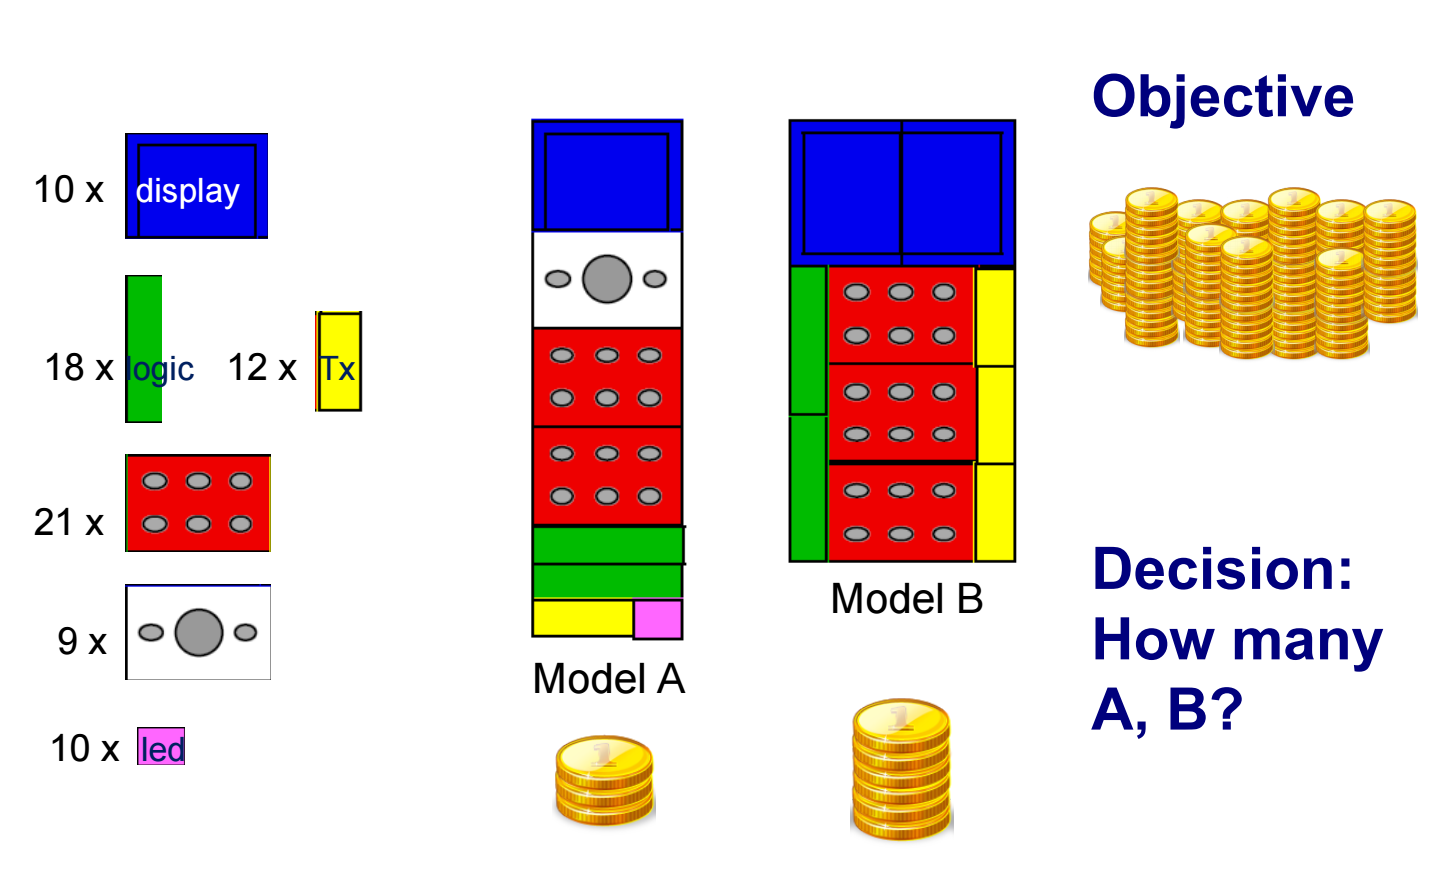
\includegraphics[width=0.7\textwidth]{images/l1-telefono.png}
\end{figure}

Per risolvere questo problema si possono usare varie strategie:

\begin{itemize}
	\item \textbf{Greedy}: scelgo di costruire il massimo numero di telefoni del modello con il prezzo più alto. Però non ho la garanzia che la soluzione trovata sia ottima.
	\item \textbf{Local search}: determino un certo numero di telefoni da produrre in modo da trovare una possibile soluzione sub-ottima per poi andare a modificare il numero di telefoni prodotti, cercando di migliorare il guadagno. Anche in questo caso non ho la garanzia che la soluzione trovata sia ottima.
	\item \textbf{Global search}: provo tutte le possibili combinazioni di telefoni che posso produrre, così facendo sono sicuro di trovare una soluzione ottima.
\end{itemize}


Un altro possibile problema è quello del contadino che possiede 12 ettari di terra dove può coltivare patate o pomodori, avendo a disposizione 70kg di semi di pomodoro, 18 tonnellate di tuberi di patate e 160 tonnellate di fertilizzante. Il contadino sa che un ettaro di campo coltivato a pomodori produce un guadagno di 3000 euro mentre uno di patate 5000. Per coltivare un ettaro a pomodori servono 7kg di semi e 10 tonnellate di fertilizzante, mentre un ettaro di patate richiede 3 tonnellate di tuberi e 20 di fertilizzante.

Questo problema è simile a quello del telefono, con la differenza che in questo caso gli ettari possono essere frazionati e quindi l'approccio combinatorio non può essere utilizzato.

L'idea è quindi quella di formulare un modello che descrive la soluzione ottima, anziché formulare un algoritmo che lo risolve.

Come prima cosa è necessario identificare le \textbf{variabili decisionali}, in questo caso $x_T$ e $x_P$ che rappresentano gli ettari coltivati. 
Poi si deve definire la \textbf{funzione obiettivo} che si vuole ottimizzare, in questo caso $\max 3000 x_T + 5000 x_P$.
Infine è necessario definire i \textbf{vincoli del problema} per modellare il consumo di risorse. In questo caso:

\begin{align*}
	x_T + x_P &\leq 12 \text{ vincolo sulla terra} \\
	7 x_T &\leq 70   \text{ vincolo sui semi di pomodoro} \\
	3 x_P &\leq 18 \text{ vincolo sui tuberi} \\
	10 x_T + 20 x_P &\leq 160 \text{ vincolo sul fertilizzante} 
\end{align*}

Con questa formulazione del problema non dico niente riguardo la soluzione del problema, ma posso utilizzare il modello creato per trovarla utilizzando dei metodi matematici dato che l'insieme di vincoli può essere visto come un sistema di disequazioni.

Un primo approccio è quello di partire da un valore di partenza della funzione obiettivo, ad esempio 27000 e provare a migliorarlo utilizzando la discesa di gradiente, fino a trovare un punto del piano che corrisponde ad un valore ottimo.
Con questo approccio posso anche dire che la soluzione trovata è ottima, perché tutte le altre soluzioni migliori richiedono un maggior numero di risorse.

\begin{figure}[htbp]
	\centering
	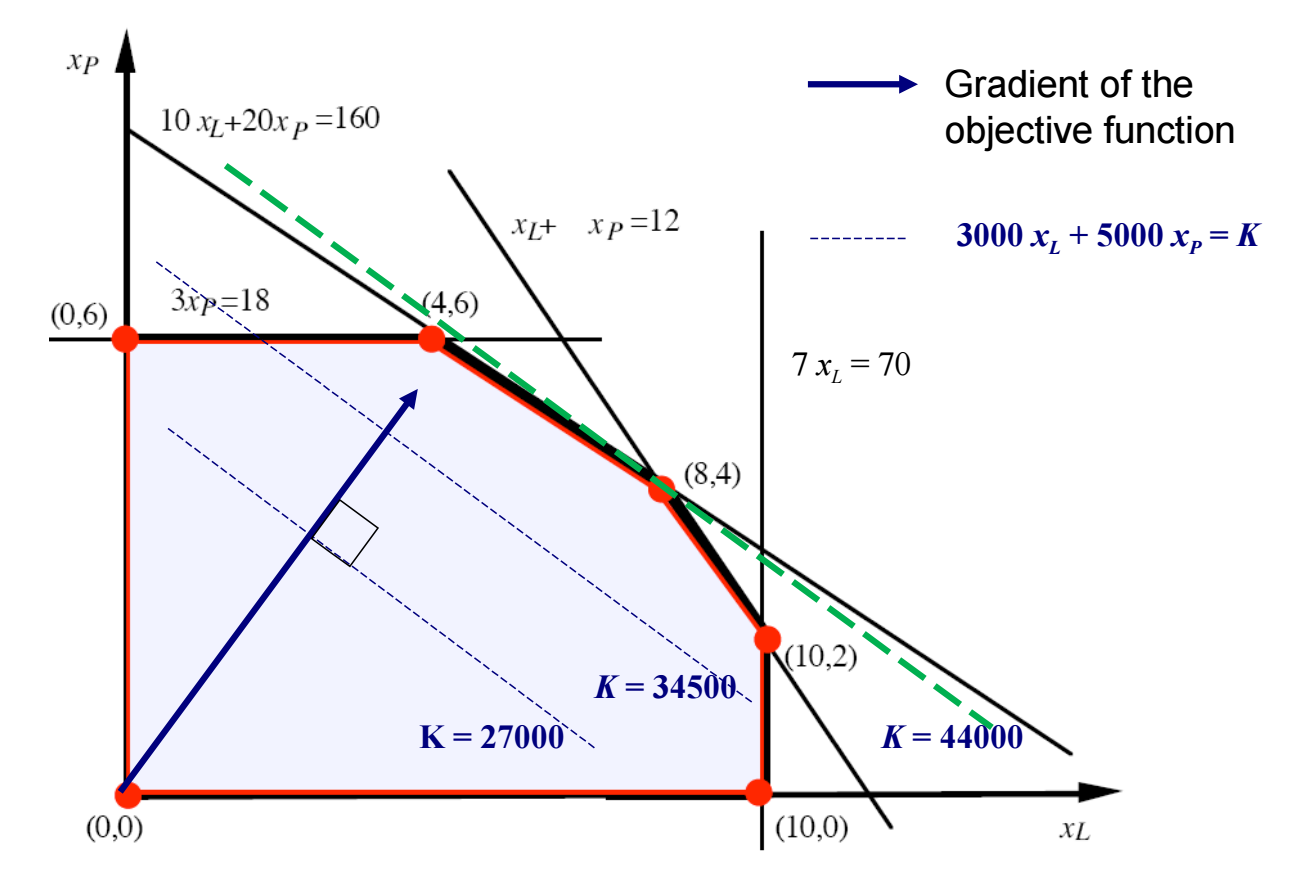
\includegraphics[width=0.5\textwidth]{images/l1-poligono.png}
\end{figure}


Tutto questo funziona perché sia i vincoli che la funzione obiettivo sono \textbf{lineari} e le variabili sono numeri reali. Questo tipo di modelli prende quindi il nome di \textbf{Linear Programming}.

Da notare che in questo caso la soluzione ottima è su un vertice intero, ma è un caso. Se le variabili utilizzate possono essere solo intere la situazione diventa più complessa perché è necessario effettuare delle approssimazioni.

\section{Approccio della ricerca operativa}

\begin{figure}[htbp]
	\centering
	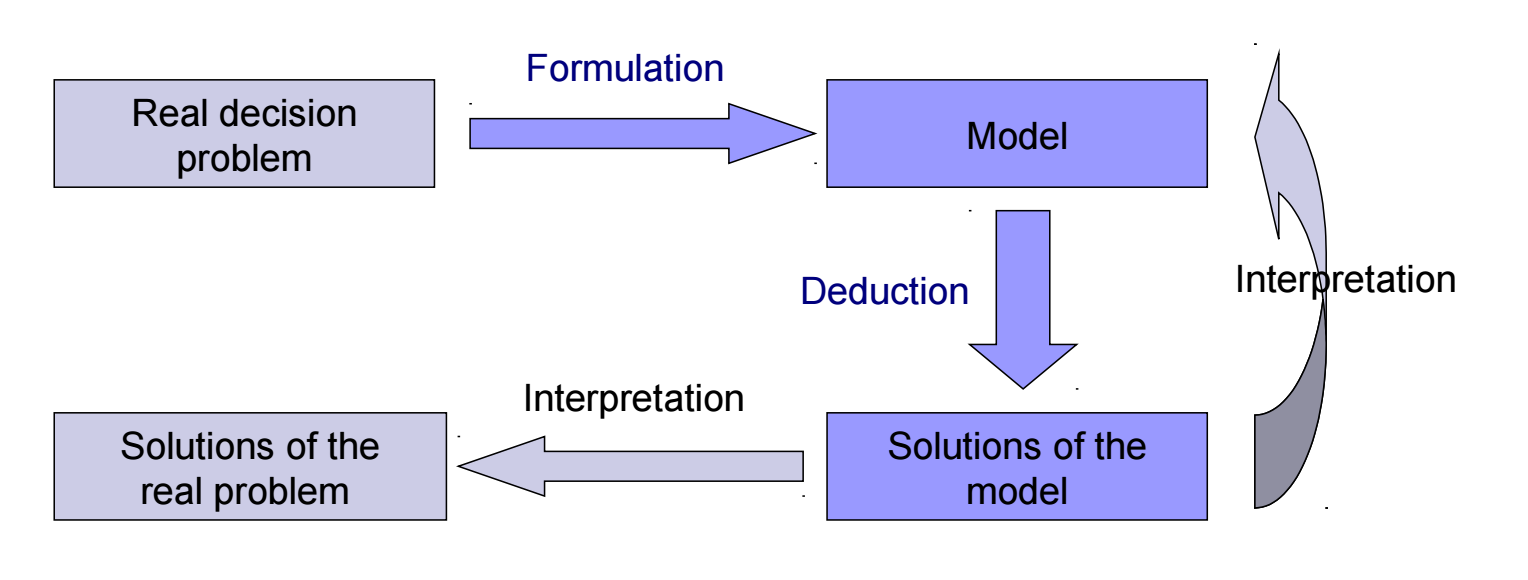
\includegraphics[width=0.7\textwidth]{images/l1-approccio.png}
\end{figure}

L'approccio precedentemente descritto è quello della ricerca operativa: si parte da un problema reale che viene formalizzato utilizzando un modello. Dal modello viene trovata una soluzione ottima per esso, la quale deve poi essere trasformata nella soluzione del problema reale.
Questo secondo passo può essere necessario perché nel modellare il problema può essere che sia stato necessario modificare alcuni vincoli, oppure utilizzare delle variabili reali anziché intere.

Si possono quindi definire due fasi: una di \textbf{formulazione} del modello e una di \textbf{deduzione} della soluzione, utilizzando alcuni algoritmi già definiti o personalizzati.

\section{Programma del corso}

\begin{enumerate}
	\item Ripasso e approfondimento delle tecniche di programmazione lineare e della dualità.
		\begin{itemize}
			\item Modelli LP, metodo del simplesso, teorema della dualità.
			\item Column generation technique per modelli LP grandi. Ovvero la creazione di modelli dinamici per evitare le limitazioni della memoria.
			\item Applicazioni: pianificazione della produzione, gestione del flusso di rete.
		\end{itemize}
	\item Metodi avanzati per la programmazione lineare intera mista (\textbf{MILP}).
		\begin{itemize}
			\item Formulazioni alternative, Branch \& Bound, Branch \& Cut.
			\item Applicazioni: Traveling Salesman Problem, localizzazione dei magazzini, set cover.
		\end{itemize}
	\item Meta euristiche per l'ottimizzazione combinatoria.
		\begin{itemize}
			\item Neighbourhood search e varianti.
			\item Algoritmi genetici.
		\end{itemize}
	\item Network optimization: modellazione dei problemi di ottimizzazione con i grafi. \textit{Potrebbe non essere affrontato.}
	\item \textbf{Laboratorio}:
		\begin{itemize}
			\item Online optimization server
			\item Optimization software and Algebraic modelling languages
			\item Optimization libraries (Cplex, Coin-OR, Scip)
		\end{itemize}
\end{enumerate}


\section{Informazioni pratiche}

Ci saranno dei laboratori nell'orario delle lezioni, verrà specificato nel sito quando ci saranno.

Non ci sono libri, vengono fornite le dispense dal professore e saranno in inglese.

Per ottenere il software che verrà utilizzato il laboratori è necessario registrarsi sul sito \url{http://www.math.unipd.it/userlist/subscribe/?idlist=277}, utilizzando la chiave \texttt{MeMoCO.16}. Per scaricare gratuitamente CPlex Optiumization Suite è necessario registrarsi alla IBM Academic Initiative.

L'esame è composto da:

\begin{itemize}
	\item Due esercitazioni di laboratorio, una sulla modellazione MILP e una sulle meta-euristiche, da consegnare qualche giorno prima dell'orale. Da fino a 10 punti.
	\item Esame orale che consiste nella discussione delle esercitazioni di laboratorio e delle domande teoriche sui contenuti del corso. Da fino a 20 punti. Forse si può fare in italiano.
	\item Progettino opzionale per ottenere un bonus da 2 a 6 punti. Il progetto riguarda la modellazione di un problema accordato con il docente e risolto utilizzando delle meta-euristiche o in modo esatto. Può essere fatto anche dopo lo scritto.
\end{itemize}



\chapter{Laboratorio}

\section{Un po' di cose su R}\label{un-po-di-cose-su-r}

\begin{itemize}
\item
  Tutti gli oggetti sono vettori
\item
  \texttt{ls()} per vedere le variabili disponibili
\item
  \texttt{x\ \textless{}-\ c(2,3,4,5)} crea un vettore con 1,2,3,4.
\item
  notazione \texttt{{[}1:20{]}} per un vettore con la successione da 1 a
  20
\item
  \texttt{xx\ \textless{}-\ seq(from=100,\ to=1)} crea sempre una
  sequenza di numeri, con parametro opzionale \texttt{by} per
  specificare lo step
\item
  \texttt{rep(2,5)} crea un vettore con 5 elementi uguali a 2
\item
  \texttt{a\ \textless{}-\ c(rep(2,3),4,5,rep(1,5))},
  \texttt{a\ =\ 2\ 2\ 2\ 4\ 5\ 1\ 1\ 1\ 1\ 1}
\item
  \texttt{2*x} esegue il prodotto scalare
\item
  \texttt{length(x)} per la lunghezza del vettore
\item
  \texttt{max(x)} e \texttt{min(x)}
\item
  \texttt{sum(x)} che ritorna un vettore di un solo elemento con la
  somma
\item
  \texttt{mean(x)}, \texttt{var(x)}, \texttt{range(x)}
\item
  \texttt{x{[}7{]}} per estrarre il settimo elemento di \texttt{x},
  l'indice credo parta da 1
\item
  \texttt{x{[}-4{]}} ritorna un vettore senza il quarto elemento
\item
  \texttt{x\ \textless{}-\ matrix(c(2,3,5,7,11,13),nrow\ =\ 3)} crea una
  matrice con gli elementi specificati e 3 righe. Alternativamente è
  possibile specificare anche il numero di colonne.
\item
  \texttt{x2\ \textless{}-\ scan("nome\ file",\ sep="")} con
  \texttt{sep} opzionale, per caricare il contenuto di un file in un
  vettore, per caricare una matrice
  \texttt{x2\ \textless{}-\ matrix(scan(...),\ ncol\ =\ 3,\ byrow=TRUE}.
\item
  \texttt{str(x)} specifica la struttura dell'oggetto
\item
  \texttt{dim(x)} ritorna la dimensione di una matrice, se invocato con
  un vettore ritorna \texttt{NULL}.
\item
  \texttt{x{[}18,{]}} per ottenere la 18-esima riga di una matrice
\item
  \textbf{Dataframe}: matrice le cui colonne possono avere formati
  diversi
\item
  \texttt{ciliegi\ \textless{}-\ read.table("nome\ file")}.
\item
  \texttt{names(ciliegi)} è il vettore con i nomi delle colonne del
  dataframe
\item
  \texttt{names(ciliegi)\ \textless{}-\ c("diametro",\ "altezza",\ "volume")}
  permette di impostare il nome delle colonne, può anche essere
  specificato come parametro opzionale \texttt{col.names} della
  funzione \texttt{read.table}.
\item
  \texttt{summary(ciliegi)} fornisce degli indicatori per ciascuna
  colonna
\item
  \textbf{Mediana}: elemento centrale di una distribuzione ordinata in
  senso crescente, \textbf{primo e terzo quartile}: generalizzazione
  della mediana, rispettivamente l'elemento che sta al 25 e 75 per cento
  della distribuzione. La differenza tra i due quartili da l'idea di
  quanto è variabile la distribuzione.
\item
  I dataframe possono essere acceduti anche con il nome della colonna
  \texttt{ciliegi\$volume}.
\item
  \textbf{attach di un file}: aggiungere al workspace un oggetto, ovvero
  \texttt{attach(ciliegi)} permette di accedere al nome della colonna
  direttamente utilizzando \texttt{volume}. Come complementare c'è il
  comando \texttt{detach}.
\item
  \texttt{hist(diametro)} crea l'istogramma per il diametro
\item
  \texttt{help(hist)} per avere l'help di una funzione
\item
  l'istrogramma che viene generato di default può contenere dei buchi,
  conviene quindi adattare il numero di colonne utilizzando il parametro
  \texttt{breaks}
\item
  \texttt{boxplot(diametro)} fornisce il box plot di un valore, è un
  grafico che rappresenta la mediana, i quartili e il 5 e 95\%. Risulta
  più espressivo dell'istogramma. L'ampiezza della scatola rappresenta
  la variabilità dei dati.
\item
  \texttt{ciliegi{[}altezza\textgreater{}80,{]}} prende tutti i ciliegi
  con altezza maggiore di 80.
\item
  \texttt{library(MASS)} permette di caricare la libreria MASS
\item
  \texttt{search()} permette di visualizzare la lista degli ottetti in
  cui R va a cercare quando deve eseguire un comando
\item
  Gli attributi qualitativi vengono trattati come tipo Factor
\item
  \texttt{table(painters\$School)} crea la tabella con le frequenze
  delle varie qualità
\item
  \texttt{barplot(..)} fa il plot delle barre per una variabile discreta
\item
  \texttt{pie(...)} fa il grafico a torta, anche se è sconsigliabile
  utilizzare un grafico a torta perché per l'occhio umano fa fatica a
  vedere la differenza tra gli angoli.
\item
  come scale colori si possono utilizzare \texttt{heat.colors(k)},
  \texttt{rainbow(k)}, \ldots{}
\item
  \texttt{plot(x,y)} disegna un diagramma di dispersione, il parametro
  \texttt{pch} specifica il tipo di carattere, \texttt{pch=16}
  rappresenta i pallini pieni, \texttt{col} specifica il colore da
  utilizzare, possono indicare \texttt{col=painter\$School} per far
  variare il colore in base al valore dell'attributo quantitativo
\end{itemize}

% !TEX encoding = UTF-8
% !TEX TS-program = pdflatex
% !TEX root = ../apprendimento_automatico.tex
% !TEX spellcheck = it-IT
\section{Lezione 5 - VC-Dimension e VC-Confidence}\label{lezione-5-vc-dimension-e-vc-confidence}

\subsection{Esempi di spazi delle ipotesi}\label{esempi-di-spazi-delle-ipotesi}

Seguono alcuni esempi di spazi per le ipotesi nei problemi di
apprendimento supervisionato, cioè quei problemi in cui si vuole
stabilire se un elemento \emph{x} appartiene o meno ad una classe.

\subsubsection{Iperpiani in R2}\label{iperpiani-in-r2}

\textbf{Iperpiano}: dato uno spazio a \emph{n}-dimensioni, un iperpiano
per quello spazio è un sottospazio di dimensione \emph{n-1}. Ad esempio gli
iperpiani in $R^2$ sono tutte le rette del piano.

Lavorando in $R^2$ lo spazio delle istanze è definito come:

$$
X = \{x | x \in R^2\}.
$$

Mentre lo spazio delle ipotesi è dato dalle dicotomie indotte da iperpiani in $R^2$, cioè da tutte le possibili divisioni del piano.

$$
H = \{f_{(w,b)}(x) | f_{(w,b)}(x) = sign(w \times x + b), w \in R^2, b \in R\}
$$

Così facendo vengono prese in considerazione tutte le rette che dividono
$R^2$ in due parti in modo che da una parte l'ipotesi valga 1 e dall'altra
-1.

\subsubsection{Dischi in $R^2$}\label{dischi-in-r2}

Sempre in $R^2$ è possibile considerare come spazio delle ipotesi tutte le
dicotomie indotte da dischi in $R^2$ e centrati nell'origine.

$$
H = \{f_b(x) | f_b(x) = sign(||x||^2 - b), w \in R^2, b \in R\}
$$

Il che vuol dire che all'interno del disco le ipotesi valgono -1 mentre
al di fuori valgono 1.

\subsubsection{\texorpdfstring{Congiunzione di \emph{m} letterali positivi}{Congiunzione di m letterali positivi}}\label{congiunzione-di-m-letterali-positivi}

Lo spazio delle istanze questa volta è dato da tutte le stringhe di \emph{m} bits

$$
X = \{s | s \in \{0,1\}^m\}
$$

Lo spazio delle ipotesi è dato da tutte le sentenze logiche che
riguardano i letterali positivi $l_1$,$l_2$,\ldots{},$l_m$ ($l_i$ è vero se
l'\emph{i}-esimo bit è 1) e che contengono solo l'operatore $\wedge$.

$$
H = \{ f_{(i_1,\ldots,i_j}(s) | f_{(i_1,\ldots,i_j}(s) \text{ equivale a } l_{i_1} \wedge l_{i_2} \wedge \ldots \wedge l_{i_j}, \{i_1\ldots{}i_j\} \text{ sottoinsieme di }  \{1..m\}\}
$$

\subsection{Misurare la complessità dello spazio delle ipotesi}\label{misurare-la-complessituxe0-dello-spazio-delle-ipotesi}

Considerato un determinato spazio delle ipotesi \emph{H}, questo
contiene sempre:

\begin{itemize}
\item
  L'\textbf{ipotesi più specifica}: ipotesi più stretta e consistente con
  i dati, nell'esempio del disco è il disco più stretto in grado di
  contenere tutti i punti negativi.
\item
  L'\textbf{ipotesi più generale}: quella più grande e consistente con i
  dati, sempre nell'esempio del disco, è quello più grande
  possibile che non contiene punti positivi.
\end{itemize}

\textbf{Shattering}: (frammentazione), dato \emph{S} sottoinsieme dello
spazio delle istanze, si dice che \emph{S} è frammentato dallo spazio
delle ipotesi \emph{H} se:

$$ 
\forall S' \in S, \exists h \in H, \text{ tale che } \forall x \in S, h(x) = 1 \text{ se e solo se } x \in S'.
$$

Cioè \emph{H} realizza tutte le possibili dicotomie di \emph{S}.

\emph{H} frammenta un certo insieme \emph{S} se è possibile trovare un
iperpiano \emph{h} che raccoglie tutti i punti dell'insieme \emph{S}. Ovvero per
tutte le dicotomie di \emph{S} esiste un iperpiano che riesce a
realizzarle.

\subsubsection{VC (Vapnik-Chervonenkis) Dimension}\label{vc-vapnik-chervonenkis-dimension}

La VC-Dimension è la dimensione di uno spazio delle ipotesi \emph{H}
definito su uno spazio delle istanze \emph{X} ed è data dalla
cardinalità del sottoinsieme più grande frammentato da \emph{H}.

$$
VC(H) =
\begin{cases}
max_{S \subseteq X} |S|&\text{ tale che \emph{H} frammenta } S  \\
 \infty& \text{ se S non è limitato}
\end{cases}
$$


Ad esempio se nello spazio delle ipotesi dato dagli iperpiani su $R^2$ ho 2 punti, lo spazio delle istanze viene frammentato da
\emph{H}, perché posso sempre trovare una retta che riesce a realizzare
tutte le possibili dicotomie di due punti su un piano.
Se nello spazio delle istanze ho 3 punti, riesco comunque a realizzare
tutte le dicotomie.
Se nello spazio delle istanze ho 4 punti qualsiasi non si riesce a
trovare un iperpiano che realizza la dicotomia, quindi \emph{VC(H) =
3}.

Segue che, prendendo uno spazio delle ipotesi di cardinalità finita si
ha che:

$$
VC(H) \leq log_2(|H|)
$$

Questo perché per ogni \emph{S} frammentato da \emph{H}, abbiamo
$|H| \geq 2^{|S|}$,
cioè per ogni dicotomia in \emph{S} esiste un ipotesi in \emph{H} che la
realizza, ovvero devono essere disponibili in \emph{H} tante ipotesi
quanti sono le dicotomie in \emph{H}.

Scegliendo un \emph{S} tale che $|S| = VC(H)$, si
ottiene $|H| \geq 2^{|S|}$, prendendo
il logaritmo si trova quello che si stava cercando, ovvero $VC(H) \leq log_2(|H|)$.

\textbf{Dal libro}:

Se un dataset contiene \emph{N} elementi, questi \emph{N} elementi
possono essere etichettati con degli 0 e 1 in $2^N$ modi diversi.

Se per ognuno di questi modi è possibile trovare un ipotesi $h \in H$
che separa tutte le istanze negative da quelle positive allora si dice
che \emph{H} frammenta il dataset \emph{N}. 
Il che vuol dire che il dataset \emph{N} può essere appreso con un errore empirico nullo.

Il massimo numero di punti che possono essere frammentati da \emph{H} è
detto \emph{VC(H)} e fornisce una misura della capacità di \emph{H}.

\subsection{Bound sull'errore di generalizzazione}\label{sec:vcc}

Considerando un problema di apprendimento binario, con:

\begin{align*}
\text{Training set }S &= \{(x_i,y_i), \ldots (x_N, y_N)\} \\
\text{Spazio delle ipotesi } H &=\{h_\theta(x)\} 
\end{align*}

Supponendo di avere un algoritmo di apprendimento \emph{L} che
restituisce l'ipotesi $h_{\theta*}$ che minimizza l'errore empirico su
\emph{S} espresso come $errore_S(h_\theta(x))$.

È possibile derivare un bound (limite superiore) per l'errore ideale o
errore di generalizzazione, valido con probabilità \emph{(1 - $\sigma$)} con
$\sigma$ piccolo a piacere:

$$
errore_D(h_\theta(x)) \leq  errore_S(h_{\theta}(x)) + g(N, VC(H), \sigma)
$$

Il primo termine $errore_S(h_{\theta}(x))$ dipende dall'ipotesi restituita
dall'algoritmo di apprendimento \textit{L}.

Il secondo termine $g(N, VC(H), \sigma)$ non dipende da \emph{L}, ma dal
numero di esempi di training utilizzati (inversamente proporzionale),
dalla \emph{VC-dimension} (direttamente proporzionale) e dalla
confidenza, ovvero dal termine $\sigma$.

Questo termine viene anche chiamato \textbf{VC-confidence} e risulta essere monotono rispetto al rapporto
$\frac{VC(H)}{N}$.

\textbf{Morale della favola}: la VC-Dimension sovrastima con confidenza $\sigma$ l'errore ideale.

\subsection{Structural Risk Minimization (SRM)}\label{sec:srm}

Approccio per la scelta dello spazio delle ipotesi proposto da Vapnik
che cerca di trovare un compromesso tra l'errore empirico e la
VC-Confidence.

Si considerano spazi delle ipotesi sempre più piccoli $H_1 \subseteq H2 \subseteq \ldots \subseteq H_n$ tali che $ VC(H_1) \leq VC(H_2) \leq \ldots \leq VC(H_n)$

Si seleziona lo spazio delle ipotesi $H_i$ che ha il valore del bound
sull'errore di generalizzazione più piccolo. ovvero la VC-Dimension minore.

\begin{figure}[htbp]
\centering
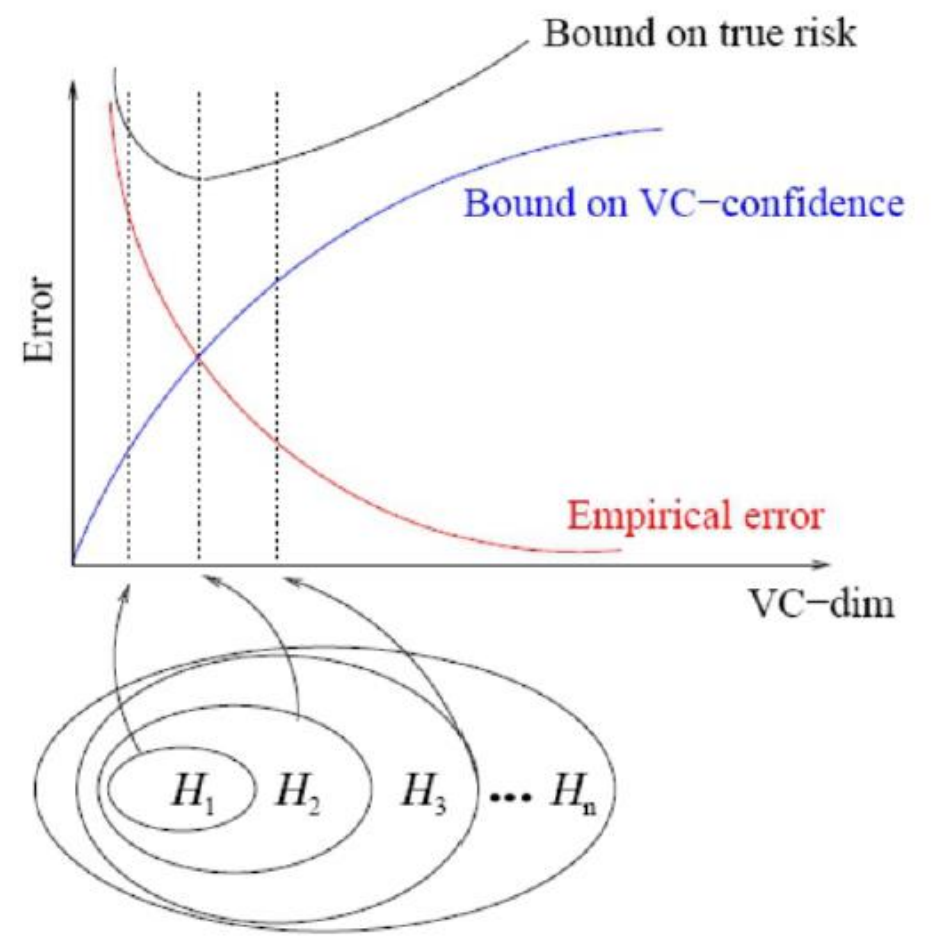
\includegraphics[width=0.5\textwidth]{./notes/immagini/l5-srm.png}
\caption{Structural Risk Minimization}
\end{figure}

% !TEX encoding = UTF-8
% !TEX program = pdflatex
% !TEX root = AALP.tex
% !TEX spellcheck = it-IT

% 27 Ottobre 2016
%\section{Estensioni del nostro linguaggio}
%\subsection{Record}
% \subsubsection{L'oggetto conto}

\section{Tipi variante}

Se i record possono essere visti come tipi congiunzione, che combinano più tipi, i tipi variante possono essere visti come disgiunzione.

Ad esempio possiamo pensare ad un contatto in una rubrica che può avere un indirizzo fisico o virtuale:

$$
< \text{fisico}: \underbrace{\{ \text{nome : String}, \text{indirizzo: String} \}}_{T_{fisico}} , \: \text{virtuale}: \underbrace{\{ \text{login : String}, \text{email : String} \}}_{T_{virt}} >= T_{ind}
$$

\noindent Un esempio di valore che ha questo tipo è:

$$
< \text{fisico} = \{ \text{nome = ``pippo''}, \text{indirizzo =  ``Via rosa''} \} >
$$

\noindent L'utilità di questi tipi si ha con l'operatore di pattern matching.
Ad esempio in Scala è possibile definire delle funzione generiche che lavorano sui tipi variante:

\begin{lstlisting}[language=Scala, caption=Utilizzo del pattern matching in Scala]
def getName(a : Tind) : String = a match{
	case <fisico = x> => x.nome
	case <virtuale = x> => x.login
	/** case <l = x> => ... da errore di compilazione! */
	/** allo stesso modo viene segnalato se il pattern non copre tutte le possibili etichette */
}

def getAll(a : List[Tind] ) : List[String] = {
	var l = new List[String]
	for (x <- a) l.add(getName(x))
}
\end{lstlisting}

\noindent Per inserire nel nostro linguaggio questi valori servono dei nuovi termini:

$$
M ::= < l = M > \vbar M \text{ match } \{\text{case }l_i = x_i => M_i \:^{i = 1\ldots n}\} \vbar \ldots
$$

\noindent Da notare che la $x_i$ che viene utilizzata nel \text{match} lega le eventuali occorrenze all'interno di $M_i$.

$$
<l_1 = 3> \text{ match } \{\text{case } l_1 = x => x+1, \ldots \} \rightarrow 3+1
$$

\noindent Più formalmente:

\begin{itemize}
	\item $fv(<l =M>) = fv(M)$
	\item $fv( M \text{ match } \{\text{case }l_i = x_i => M_i \:^{i = 1\ldots n}\}) = fv(M) \cup \bigcup_{i = 1 \ldots n}\bigg( fv(M_i) \setminus \{x_i\} \bigg) $
\end{itemize}


\noindent Servono inoltre dei nuovi valori finali e dei tipi:

$$
v ::= <l = v> \vbar \ldots \qquad T ::= < l_i : T_i \:^{i = 1 \ldots n}>
$$

\noindent La semantica operazionale viene espressa con 3 nuove regole:

\begin{itemize}
	\item Riduzione del termine interno
	\begin{prooftree}
		\AxiomC{$M \rightarrow M'$}
		\LL{Variant}
		\UnaryInfC{$<l = M> \rightarrow <l = M'>$}
	\end{prooftree}
	\item Avanzamento in un match:
	\begin{prooftree}
		\AxiomC{$M \rightarrow M'$}
		\LL{Red-Match}
		\UnaryInfC{$M \text{ match } \{\text{case } l_i = x_i => M_i \:^{i = 1 \ldots n}\} \to M' \text{ match } \{\text{case } l_i = x_i => M_i \:^{i = 1 \ldots n}\}$}
	\end{prooftree}
	\item Assioma per il match effettivo
	\begin{prooftree}
		\AxiomC{$j \in \{1 \ldots n\}$}
		\LL{Match}
		\UnaryInfC{$<l_j = v> \text{ match } \{\text{case } l_i = x_i => M_i \:^{i = 1 \ldots n}\} \rightarrow M_j\{x_j = v\}$}
	\end{prooftree}
\end{itemize}

\noindent Servono inoltre delle regole di tipo, una per l'invariante e l'altra per il match.

\begin{prooftree}
	\AxiomC{$ \Gamma \vdash M: T_j $}
	\AxiomC{$ j \in \{1 \ldots n \} $}
	\LL{Type-Variant}
	\BinaryInfC{$\Gamma \vdash <l_j = M> : <l_i : T_i \:^{i=1\ldots n}>$}
\end{prooftree}

\noindent Con questa regola posso assegnare ad un valore infiniti tipi, l'importante è che in questi infiniti tipi ci sia l'etichetta $l_j$ in modo da avere la garanzia di riuscire ad effettuare il pattern matching.

\begin{prooftree}
	\AxiomC{$\Gamma \vdash M : < l_i : T_i  \:^{i=1\ldots n}>$}
	\AxiomC{$\Gamma, x_i : T_i \vdash M_i : T \:\: \forall \: i = 1 \ldots n $}
	\LL{Type-Match}
	\BinaryInfC{$\Gamma \vdash M \text{ match }\{\text{case }l_i = x_i => M_i \:^{i=1\ldots n}\} : T$}
\end{prooftree}

\noindent Perché un match sia ben tipato è necessario che il termine $M$ sia un valore di tipo variante e che tutti i ``rami'' del match siano termini con lo stesso tipo, aggiungendo anche al contesto la sostituzione che viene effettuata quando viene applicato il match.

Se nel pattern matching ho come premessa della regola $\Gamma \vdash M : < l_i : T_i  \:^{i=1\ldots m}>$ con $m \geq n$ c'è un problema perché possono capitare delle etichette che il costrutto \text{match} non riesce a gestire. Se invece $m \leq n$ non ci sono problemi. Ma anche in questo caso, dato che ho a disposizione infiniti tipi, conviene forzare $m = n$.

Anche se non sembra questi tipi sono presenti nella maggior parte dei linguaggi main stream, solo che questi vengono nascosti da dello zucchero sintattico. Ad esempio le liste possono essere viste come un tipo variante in quanto sono o una lista vuota o la concatenazione di un elemento e un'altra lista.

$$
\text{List} = < \text{nil : Unit}, \text{cons} : (\Nat * \text{List}) >
$$

\noindent Si tratta di un tipo ricorsivo che non è supportato nella nostra grammatica, ma in altre grammatiche è possibile gestirlo.

I valori per questo tipo sono:

$$
<\text{nil } = \text{unit}>  \quad <\text{cons} = (5, <\text{nil } = \text{unit}>)>
$$

\noindent Un altro caso d'uso dei valori variante è l'analisi delle dereferenziazioni dei valori null.
Ad esempio in Java possiamo definire una variabile e assegnarle null:

\begin{lstlisting}[language=Java]
C c = null;

C find(List<C> l, C a) { ... } // se non trova ritorna null

C c = find(list, s);
// c può essere null, quindi devo controllare
// se non controllo potrei finire in un NullPointerException, anche perché il compilatore non controlla questo tipo di eccezioni
if (c != null) print(c.info());
else print("non trovato");
\end{lstlisting}

\noindent Questo approccio non è dei migliori, perché dovrebbe utilizzare le eccezioni personalizzate, ma si è visto che nessuno le usa. Con C\# si sono invece inventati i tipi \texttt{Nullable} che possono avere anche come valore \texttt{Null}, anche per i tipi primitivi.

Un'altra idea è stata quella di introdurre i tipi \texttt{!}: una classe di tipo \texttt{C!} non può assumere come valore null, in modo da sfruttare di più l'analisi statica.

Linguaggio che vai, soluzione che trovi. Altri linguaggi utilizzano i così detti \textbf{null objects}:

\begin{lstlisting}[language=Java]
class C {
	...
	String info() {...}
	...
}
class NullC extends C {
	...
	String info() {}
}
\end{lstlisting}

\noindent Così facendo c'è un metodo definito da chiamare anche sul valore null, in modo da evitare la NullPointerExcpetion.

Scala e Java8 (e Swift) implementano un'ulteriore versione, gli \textbf{option type}, ovvero un tipo variante che prevede due possibilità: c'è l'oggetto oppure non c'è.
La definizione di questo tipo è la seguente:

$$
Option[C] = < \text{none} : \text{Unit}, \text{some} : C >
$$

\noindent Il codice di prima può essere quindi riscritto come

\begin{lstlisting}[language=Scala]
...
def find(l : List[C], s : String) : Option[C] = {
	for(x <- l) 
		if (x.info() == s) return Some(x)
	return None 
}
...
find(l, "pippo") match {
	case Some(x) => print(x.info())
	case None => print("non trovato")
}
\end{lstlisting}

\noindent Si può notare come questa versione del codice è più espressiva e si riesce subito a capire che la funzione \texttt{find} può non trovare l'elemento cercato.



% !TEX encoding = UTF-8
% !TEX TS-program = pdflatex
% !TEX root = computabilità e algoritmi.tex
% !TEX spellcheck = it-IT
\section{Composizione generalizzata}\label{composizione-generalizzata}

$$f: \mathbb{N}^k \rightarrow \mathbb{N},\: g_1,\ldots g_n : \mathbb{N}^k \rightarrow \mathbb{N}$$

La loro composizione $h: \mathbb{N}^k \rightarrow \mathbb{N}$ è data da: 

$$
h(\vec{x}) = f(g_1(\vec{x}), \ldots, g_n(\vec{x}))
$$

La funzione $h(\vec{x})\downarrow$ (è definita) se tutte le
$g_i \downarrow y_i, f(y_1,\ldots,y_n) \downarrow$.

L'approccio utilizzato nella valutazione delle funzioni è quello
\textbf{eager}, ovvero vengono valutati prima tutti i parametri.

Ad esempio: $\underline{0} : \mathbb{N} \rightarrow \mathbb{N},\: \underline{0}(x) = 0$ e $d(x) = \uparrow,\: \underline{0}(d(1))$ è
$\uparrow$ perché prima è necessario valutare i parametri.

\subsection{Calcolabilità della funzione
composta}\label{calcolabilituxe0-della-funzione-composta}

Se $f: \mathbb{N}^n \rightarrow \mathbb{N}, g_1\ldots g_n : \mathbb{N}^k \rightarrow \mathbb{N} \in \mathcal{C}$, allora anche $h: \mathbb{N}^k \rightarrow \mathbb{N}$ è calcolabile in $\mathcal{C}$.

\subsubsection{Dimostrazione}\label{dimostrazione}

Siano $F,G_1, \ldots{}, G_n$ programmi URM in forma normale per
le relative funzioni.

L'input della funzione \emph{h} avrà nei primi \emph{k} registri i
valori di input, è necessario quindi andare a copiarli in una locazione
di memoria che non viene usata dai vari programmi, ovvero dalla
locazione \emph{m+1}, con $m = max\{\rho(F), \rho(G_1), \ldots \rho(G_N), k,n\}$.

I risultati parziali dei programmi vengono poi memorizzati a partire
dalla locazione \emph{m + k +1} per poi essere utilizzati da \emph{F}

Il programma risultante è:

\begin{lstlisting}[language=URM]
T([1 ... k],[m+1 ... m+k])
G1[m+1 ... m+k -> m+k+1]
...
Gn[m+1 ... m+k -> m+k+n]
F[m+k+1 ... m+k+n -> 1]
\end{lstlisting}

\subsubsection{Esempio - Somma di due numeri}\label{esempio}

A partire dalla funzione $sum(x_1, x_2) = x_1+x_2$ è possibile andare a ottenere la funzione

$$f(x_1, x_2, x_3) = x_1 + x_2 +x_3$$

componendo la funzione \textit{sum} con se stessa:

$$f(x_1, x_2, x_3) = sum(sum(x_1,x_2),x_3)$$

Tuttavia, strettamente parlando, le $g_i$ non hanno la stessa
arietà, pertanto sono necessari dei piccoli aggiustamenti:

$$f(x_1, x_2, x_3) = sum(sum(U_1^{3}(\vec{x}),U_2^3(\vec{x}))), U_3^3(\vec{x}))$$

\section{Ricorsione Primitiva}\label{ricorsione-primitiva}

\begin{align*}
	fact(0) &= 1 \\
	fact(n+1) &= (n+1)fact(n)
\end{align*}

\begin{align*}
	fib(0) &= 1 \\
	fib(1) &= 1 \\
	fib(n+2) &= fib(n+1) + fib(n)
\end{align*}

Date $f: \mathbb{N}^k \rightarrow \mathbb{N}$ e $g:\mathbb{N}^{k+2} \rightarrow \mathbb{N}$, la funzione per ricorsione primitiva $h: \mathbb{N}^{k+1} \rightarrow \mathbb{N}$ è definita come

\begin{align*}
	h(\vec{x}, 0) &= f(x) \\
	h(\vec{x}, y+1) &= g(\vec{x}, y, h(\vec{x},y))
\end{align*}

Così facendo viene definita \emph{h} utilizzando \emph{h} e
concettualmente è corretto, tuttavia è necessario dimostrare formalmente
l'esistenza e l'unicità di \emph{h}.

Questo lo si fa considerando l'operatore $\Phi$:

\begin{align*}
	\Phi : (\mathbb{N}^k \rightarrow \mathbb{N}) &\rightarrow (\mathbb{N}^k \rightarrow \mathbb{N}) \\
	\Phi(h)(\vec{x}, 0) &= f(\vec{x}) \\
	\Phi(h)(\vec{x}, y+1) &= g(\vec{x}, y, h(\vec{x},y))
\end{align*}

tale che $\Phi(h) = h$, ovvero tale che viene raggiunto un punto
fisso. Ciò sarebbe da dimostrare, ma questo va oltre l'obiettivo del corso, quindi viene dato per buono.

In altre parole, se \emph{h} rispetta lo schema precedentemente definito, allora esiste ed è unica.

Assumendo quindi che la ricorsione primitiva di una funzione calcolabili
è calcolabile, è possibile definire varie operazioni senza scrivere
esplicitamente il programma per calcolarle:

Ad esempio la funzione somma può essere definita in modo ricorsivo:

$$
	x+y = h(x,y) =\begin{cases}
	x+0 = x &\Rightarrow f(x) = x \\
	x+(y+1) = (x+y) + 1 &\Rightarrow g(x,y,z) = succ(z)
	\end{cases}
$$

In modo simile possono essere anche definiti il prodotto e l'esponenziale:

$$
x \cdot y = h(x,y) =\begin{cases}
x \cdot 0 = 0 &\Rightarrow f(x) = 0 \\
x \cdot (y+1) = (x \cdot y) + x &\Rightarrow g(x,y,z) = z+x
\end{cases}
$$

$$
x^y = h(x,y) =\begin{cases}
x^0 = 1 &\Rightarrow f(x) = 1 \\
x^{(y+1)} = (x^y) \cdot x &\Rightarrow g(x,y,z) = z \cdot x
\end{cases}
$$

\subsection{Calcolabilità della Ricorsione Primitiva}\label{calcolabilituxe0-della-ricorsione-primitiva}

Siano $f:\mathbb{N}^k \rightarrow \mathbb{N}$ e $g:\mathbb{N}^{k+2} \rightarrow \mathbb{N} \in \mathcal{C}$ allora anche \emph{h} definita per
ricorsione primitiva è in $\mathcal{C}$. Ovvero quello che è stato assunto precedentemente.

\subsubsection{Dimostrazione}\label{dimostrazione-1}

Siano \emph{F} e \emph{G} i programmi che calcolano \emph{f} e \emph{g}.

Il programma che calcola \emph{h} verrà invocato con il vettore \emph{x}
nelle prime \emph{k} locazioni e con \emph{y} nella locazione
\emph{k+1}.

Come prima cosa è necessario trasferire i dati di input in una zona di
memoria non utilizzata dai programmi \emph{F} e \emph{G}, ovvero
\emph{m+1}, dove $m = max\{\rho(F), \rho(G), k+2\}$.

Dopodiché è necessario effettuare un'interazione su un contatore
\emph{i} che parte da 0, fino a quando non viene raggiunto \emph{y}.

\begin{verbatim}
h(vec(x), 0) = f(vec(x)) -- i=0 -- i==y? NO
h(vec(x), 1) = g(vec(x), 0, h(vec(x),0)) -- i=1 -- i==y? NO
...
h(vec(x), i+1) = g(vec(x), i, h(vec(x),i)) -- i=n -- i==y? SI -> fine
\end{verbatim}

ovvero il programma per \emph{h} sarà:

\begin{lstlisting}[language=URM]
T([1..k], [m+1 ... m+k]) // copia x
T(k+1, m+k+3) //copia y
F[m+1 ... m+k -> m+k+2]
J(m+k+3, m+k+1, END) #LOOP
G[m+1 ... m+k+2 -> m+k+2] // h(vec(x),i+1)
S(m+k+1) //i++
J(1,1,LOOP)
T(m+k+2,1) #END
\end{lstlisting}

Se \emph{f} e \emph{g} sono funzioni parziali quanto dimostrato richiede
maggiori precisazioni, ma a noi basta sapere che se durante il calcolo
troviamo qualche funzione non definita, anche \emph{h} non è definita.

\subsection{Funzioni totali definite ricorsivamente}\label{osservazione-senza-titolo}

Le funzioni definite a parte da funzioni totali mediante composizione o
ricorsione sono anche loro totali.

La dimostrazione per le funzioni mediante composizione è vera per
definizione, l'altra è lasciata per esercizio (si fa per induzione).

\todo[inline]{todo}

\subsection{Esercizio - Libreria di funzioni calcolabili}\label{esercizio---libreria-di-funzioni-calcolabili}

\begin{itemize}
\item
  somma \emph{x+y}
\item
  prodotto $x \cdot y$
\item
  esponenziale $x^y$
\item
  fattoriale \emph{fact(x)}
\end{itemize}

Sguardo d'insieme: vogliamo trovare un programma URM in grado di
simulare un altro programma URM, le operazioni numeriche sono
interessanti perché il programma in input verrà rappresentato come un
numero.

\subsubsection{Predecessore}\label{predecessore}

$$ \text{pred}(x) = \begin{cases}x \dotminus 1 = 0, \:& \text{ se } x=0\\
x-1, \:& \text{ se } x > 0\end{cases}$$

Può essere calcolata ricorsivamente con

\begin{align*}
	0 \dotminus 1 &= 0 \\
	(y+1) \dotminus 1 &= y
\end{align*}

\subsubsection{Sottrazione tra numeri naturali}\label{sottrazione-tra-numeri-naturali}

$$x \dotminus y =\begin{cases}
0,\:& \text{se } x \leq y\\
x-y, \:& \text{altrimenti}
\end{cases}$$

Può essere calcolata ricorsivamente con:

\begin{align*}
x \dotminus 0 &= x \\
x\dotminus (y+1) &= (x \dotminus y) \dotminus 1
\end{align*}

\subsubsection{Segno}\label{segno}

$$sg(x) =\begin{cases}
0,\:& \text{se } x = 0\\
1, \:& \text{altrimenti}
\end{cases}$$

Può essere calcolata ricorsivamente con:

\begin{align*}
sg(0) &= 0 \\
sg(y+1) &= 1
\end{align*}

In modo simile può essere definito anche $\overline{sg}$.

\subsubsection{Valore assoluto della differenza}\label{valore-assoluto-della-differenza}

$$|x - y|=\begin{cases}
x-y,\:& \text{se } x \leq y\\
y-x, \:& \text{altrimenti}
\end{cases}$$

Può essere calcolata in modo composizionale con:

$$|x - y| = (x \dotminus y) + (y \dotminus x)$$


\subsubsection{Minimo}\label{minimo}

$$ \min (x,y) =\begin{cases}
x,\:& \text{se } x \leq y\\
y, \:& \text{altrimenti}
\end{cases}$$

Può essere calcolata con:

$$\min(x,y) = x \dotminus (x \dotminus y)$$

Questo perché se \emph{x} è il minimo, $x\dotminus y$ è 0.

\subsubsection{Resto della divisione intera}\label{resto-della-divisione-intera}

$$\text{rm}(x,y) =\begin{cases}
y \mod x,\:& \text{se } x \neq y\\
y, \:& \text{altrimenti}
\end{cases}$$


Può essere calcolato ricorsivamente come:

\begin{align*}
\text{rm}(x,0) &= 0 \\
\text{rm}(x, y+1) &= \begin{cases}\text{rm}(x+y) +1, \:& \text{ se rm}(x+y) +1 \neq x\\
0, \:& \text{ altrimenti} \end{cases}
\end{align*}

L'\emph{if} può essere espresso in modo algebrico utilizzando la
funzione \emph{sg}, ottenendo:

$$\text{rm}(x, y+1) = (sg(x \dotminus \text{rm}(x,y) \dotminus 1))(\text{rm}(x,y)+1)$$

\subsubsection{Esercizio - Divisione intera}\label{esercizio---divisione-intera}

$$\text{qt}(x,y) =\begin{cases}
\floor[\Big]{\frac{y}{x}},\:& \text{se } x \neq y\\
y, \:& \text{altrimenti}
\end{cases}$$

\todo[inline]{todo}

\subsubsection{Esercizio - Definizione per casi}\label{esercizio---definzione-per-casi}

$f_1 \ldots f_n : \mathbb{N}^k \rightarrow \mathbb{N}$ totali e calcolabili e
$Q_1, \ldots, Q_n \subseteq \mathbb{N}^k$ decidibili e tali che per ogni $\vec{x}$ solo un predicato è vero.

Definire $f(x) = f_1(x) \text{ se } Q_1(x) \ldots f_n(x) \text{ se } Q_n(x)$

\todo[inline]{todo}

% !TEX encoding = UTF-8
% !TEX TS-program = pdflatex
% !TEX root = computabilità e algoritmi.tex
% !TEX spellcheck = it-IT
\paragraph{Soluzione}\label{soluzione-esercizio}

La funzione \emph{f(x)} viene definita per casi e dal momento che i vari
predicati sono decidibili ed esaustivi, quindi almeno uno dei casi è
vero.

$$
f(\vec{x}) = f_1(\vec{x}))\cdot \mathcal{X}_{Q_1} + \ldots +	 f_m(\vec{x}))\cdot \mathcal{X}_{Q_m}
$$

Quando un caso è vero, viene calcolata la funzione associata, che è
totale. Se questa funzione non fosse totale, potrebbe essere che il
predicato vero su un certo \emph{x}, ma che la funzione su
quell'\emph{x} non sia definita e quindi neanche \emph{f(x)}
risulterebbe definita, perdendo così la totalità.

La calcolabilità deriva dal fatto che la definizione per casi viene
fatta con una serie di \emph{if} che è dimostrato essere calcolabile e
le funzioni $\mathcal{X}_{Q_i}$ sono calcolabili, perché i predicati sono
decidibili.

\subsubsection{Algebra della decidibilità}\label{algebra-della-decibilituxe0}

I predicati decidibili sono chiusi rispetto negazione, congiunzione e
disgiunzione.

Ovvero se \textit{Q} e \textit{Q'} sono due predicati in $\mathbb{N}^k$ decidibili allora anche:

\begin{enumerate}
\item $\neg Q(\vec(x))$
\item $ Q(\vec{x}) \wedge Q'(\vec{x})$
\item $ Q(\vec{x}) \vee Q'(\vec{x}) $
\end{enumerate}

Questo perché le relative funzioni che li calcolano possono essere definite come:

\begin{enumerate}
	\item $ \mathcal{X_{\neg Q}}(\vec{x}) = \overline{sg}( \mathcal{X_{Q}}(\vec{x})) $
	\item $ \mathcal{X_{Q \wedge Q'}}(\vec{x})= \mathcal{X_{Q}}(\vec{x}) \cdot \mathcal{X_{Q'}}(\vec{x})$
	\item $ \mathcal{X_{Q \vee Q'}}(\vec{x})= sg(\mathcal{X_{Q}}(\vec{x}) + \mathcal{X_{Q'}}(\vec{x}))$
\end{enumerate}

Tutte le funzioni così definite sono calcolabili perché ottenute da composizioni di funzioni calcolabili.

\subsubsection{Somma e prodotto dei valori di una funzione}

Data una funzione totale e $ f : \mathbb{N}^{k+1} \rightarrow  \mathbb{N}$ totale e calcolabile, è possibile definire le due funzioni che effettuano la somma e il prodotto dei primi \textit{y} valori della funzione.

\begin{align*}
	s(\vec{x}, y) &= \sum_{z < y} f(\vec{x},z) \\
	p(\vec{x}, y) &= \prod_{z < y} f(\vec{x},z) 
\end{align*}

Entrambe le funzioni sono calcolabili e totali perché possono essere definite induttivamente (ricorsivamente) a partire da delle funzioni calcolabili.

\begin{align*}
s(\vec{x}, y) &= \begin{cases} \sum_{z < 0}f(\vec{x},z) = 0, &\text{ se $ y = 0 $} \\
\sum_{z < y+1}f(\vec{x},z) = \sum_{z < y}f(\vec{x},z) + f(\vec{x},z), &\text{ altrimenti}
\end{cases} \\
p(\vec{x}, y) &=  \begin{cases} \prod_{z < 0}f(\vec{x},z) = 1, &\text{ se $ y = 0 $} \\
\prod_{z < y+1}f(\vec{x},z) = \prod_{z < y}f(\vec{x},z) \cdot f(\vec{x},z) &\text{ altrimenti}
\end{cases}
\end{align*}

La totalità deriva dal fatto che \textit{f} è totale.

\subsubsection{Quantificazione limitata}

Combinando algebra della decidibilità e quanto detto nel paragrafo precedente è possibile la decidibilità di $ \forall $ e $ \exists $.

Dato un predicato $ Q(\vec{x},z) $ per calcolare se $ \forall z < y, Q(\vec{x},z) $ è possibile utilizzare la funzione:

$$
\mathcal{X}_{Q_\forall} = \prod_{z < y} \mathcal{X}_Q(\vec{x},z)
$$

In modo simile è possibile calcolare $ \exists z < y, Q(\vec{x},z) $:

$$
\mathcal{X}_{Q_\exists} = sg(\sum_{z < y} \mathcal{X}_Q(\vec{x},z))
$$

Trattandosi della composizione di funzioni calcolabili e totali, le funzioni così ottenute sono a loro volta calcolabili e totali.

\section{Minimalizzazione limitata}

Data una funzione $ f(\vec{x},z) : \mathbb{N}^{k+1} \rightarrow \mathbb{N}$ calcolabile e totale è possibile definire una funzione 

$$
h(\vec{x},y) = \mu z< y | f(\vec{x},z) = 0
$$

$ h $ è ancora una funzione $ \mathbb{N}^{k+1} \rightarrow \mathbb{N} $ e viene calcolata come il minimo valore di \textit{z} minore di \textit{y} e tale che $ f(\vec{x},z) $ sia uguale a 0 (tipicamente l'uguale a 0 viene omesso). 

La definizione più precisa è:

$$
h(\vec{x}, y) = \mu z < y . f(\vec{x},z) = \begin{cases}
\text{minimo $ z < y $ tale che $f(\vec{x},z) = 0$ se questo esiste} \\
y, \text{altrimenti}
\end{cases}
$$

Per come è definita, questa funzione risulta essere \textbf{totale} e \textbf{calcolabile}.
Intuitivamente è calcolabile perché si tratta di calcolare \textit{f} per vari valori, serve però una dimostrazione più formale, fatta per ricorsione primitiva.

\begin{align*}
	h(\vec{x}, 0) &= 0\\
	h(\vec{x}, y+1) &= 	\begin{cases}
										h(\vec{x},y) < y, &\text{\textit{f} si annulla su un valore minore di \textit{y}, viene resituito $ h(\vec{x},y) $}\\
										h(\vec{x},y) = y, &\text{per tutti i valori di minori \textit{y} non c'è uno 0 } \begin{cases}
										\text{se } f(\vec{x},y) = 0 \rightarrow y \\ 
										\text{se } f(\vec{x},y) \neq 0 \rightarrow y+1
										\end{cases}
										\end{cases}
\end{align*}

La seconda parte può essere facilmente tradotta nell'espressione

$$
(y \dotminus h(\vec{x},y)) \cdot (h(\vec{x},y)) + \overline{sg}(y \dotminus h(\vec{x},y)) \cdot (y + sg(f(\vec{x},y)))
$$

Dal momento che la funzione \textit{h} può essere definita per ricorsione primitiva e per composizione di funzioni calcolabili, anche lei è calcolabile.

\subsection{Funzioni calcolabili per ricorsione limitata}

Utilizzando la ricorsione limitata è possibile dimostrare la calcolabilità di varie funzioni.

\subsubsection{Numero di divisori di $x$}

\begin{align*}
	D(x) &= \text{\# divisori di } x \\
			&= \sum_{y \leq x}(\overline{sg}(rm(y,x))) 
\end{align*}

Dove \textit{rm} è la funzione resto, precedentemente dimostrata calcolabile.

\subsubsection{Numeri primi}

Dimostrare la calcolabilità dei funzioni che lavorano con i numeri primi è importante perché torneranno utili in futuro.

\begin{align*}
	Pr(x) &= \text{``$x$ è primo ''} \\
			 &= \overline{sg}(|D(x) - 2|)
\end{align*}

\begin{align*}
	P_x &= \text{``$x$-esimo numero primo, per convezione: ''} P_0 = 0, P_1 = 2, \ldots \\
	&= \begin{cases}
	P_0 = 0& \\
	P_{x+1} = \mu z \leq (P_x! + 1) \: | Pr(z) \cdot \underbrace{\overline{sg}(P_x +1 \dotminus z)}_{1 \text{ se } z > P_x  } \dotminus 1| &
	\end{cases}
\end{align*}

\begin{align*}
	(x)_y 	&= \text{esponente di  } P_y \text{ nella decomposizione di } y \\
			   &= \text{max } z \: P_{y}^z \text{ divide } x \rightarrow \mu z \leq x \text{ tale che } P_{y}^{z+1} \text{ non divide } x \\
			   &= \mu z \leq x \: \overline{sg}(rm(P_{y}^{z+1},x))
\end{align*}

\subsubsection{Esercizio - mcm, MCD, radice di x}

Dimostrare che sono calcolabili:

\begin{itemize}
	\item $ floor(\sqrt{x}) $
	\item $mcm(x,y))$
	\item $MCD(x,y)$
\end{itemize}


\section{Codifica di coppie}

La funzione di \textit{fibonacci} non può essere definita per ricorsione primitiva, perché il passo induttivo richiede una coppia di valori precedenti.

\`{E} però possibile definire una funzione $\prod : \mathbb{N} \times \mathbb{N} \rightarrow \mathbb{N}$ che codifica il valore di una coppia in un unico numero:

$$
\prod (x,y) = 2^x(2y+1) \dotminus 1
$$

Questa funzione risulta essere biunivoca perché è possibile definire l'inversa:

$$
\prod^{-1}(x) = ((n+1)_1, \frac{1}{2}(\frac{n+1}{(n+1)_1})-1)
$$

La funzione inversa è effettiva, perché è definita in termini di componenti calcolabili, anche se la definizione di funzione calcolabile non è stata vista per funzioni $\mathbb{N} \rightarrow \mathbb{N} \times \mathbb{N}$.

Utilizzando la funzione accoppiamento, è possibile definire la funzione \textit{fib} per ricorsione primitiva:

\begin{align*}
	g(x) &= \prod(fib(x), fib(x+1)) \\
	g(0) &= \prod(fib(0), fib(1)) = \prod(1,1) = 5 \\
	g(x+1) &= \prod(fib(x+1), fib(x+2)) \\
				 &= \prod(fib(x+1, fib(x)+fib(x+1)) \\
				 &= \prod(\prod_2(g(x)),\prod(\prod_1(g(x))+\prod_2(g(x)))\\		 
\end{align*}

Dove $\prod_1$ e $\prod_2$ sono rispettivamente le funzioni per il calcolo del primo e del secondo elemento della coppia.

Così facendo è stata dimostrata la calcolabilità di \textit{g} per ricorsione primitiva, ma $fib(x) = \prod_1(g(x))$ e di conseguenza \textit{fib} è calcolabile per composizione di funzioni calcolabili.

\section{Minimalizzazione illimtata}

Data $ f : \mathbb{N}^{k+1} \rightarrow \mathbb{N} $, si vuole definire $ h : \mathbb{N}^k \rightarrow \mathbb{N} $ tale che calcoli il minimo \textit{z} che azzera la funzione \textit{f}, ovvero:

$$
h(\vec{x}) = \mu z.f(\vec{x},z)
$$

Ci sono però dei problemi se $ f(\vec{x}, z) $ è sempre diversa da zero, perché in questo caso $ h $ è $ \uparrow $.

Un altro problema si ha se la funzione è indefinita per un valore $ z' $ minore dello $ z $ che azzera la funzione. Anche in questo caso si ha che $ h $ è $ \uparrow $.

$$
h(\vec{x}) = \mu z.f(\vec{x},z) = \begin{cases}
\text{minimo \textit{z} tale che } f(\vec{x},z) = 0 \text{ se esiste e se } \forall z' < z, f(\vec{x},z')\downarrow \neq 0 \\
\uparrow \text{ altrimenti}
\end{cases}
$$

Alternativamente, definendo $ Z_{f, \vec{x}} = \{z | f(\vec{x},z) = 0 \wedge \forall z' < z f(\vec{x},z') \downarrow \} $, si ha che \textit{h} è definita come

$$
h(\vec{x}) = \begin{cases}
\min Z_{f,\vec{x}} \text{ se } Z_{f,\vec{x}} \neq \emptyset \\
\uparrow \text{ altrimenti}
\end{cases}
$$

\subsection{Esercizi}

\subsubsection{Esercizio - Radice quadrata}
Dimostrare la calcolabilità di 

$$
f(x) = \begin{cases}
\sqrt{x} \text{ se \textit{x} è un quadrato} \\
\uparrow \text{ altrimenti}
\end{cases}
$$

\paragraph{Soluzione}

L'idea è quella di trovare un \textit{y} che elevato al quadrato è uguale a \textit{x}: $ y^2 - x = 0 $.

Si ha quindi che

$$ 
f(x) = \mu y.|y^2-x|
$$

ed è calcolabile perché minimizza illimitatamente una composizione di funzione calcolabile.

\subsubsection{Esercizio teorico}

Dimostrare che se $ f : \mathbb{N} \rightarrow \mathbb{N} $ è iniettiva, calcolabile e totale, anche la sua inversa è calcolabile.

\paragraph{Soluzione}

$$
f^{-1}(x) = \begin{cases}
y, &\text{ tale che } f(y) = x \\
\uparrow, &\text{ altrimenti}  
\end{cases}
$$

$$ 
f^{-1}(x) = \mu y.|f(y)-x|
$$

Perché l'uguaglianza sia rispettata è necessario che \textit{f} sia totale, dal momento che se per un certo \textit{y}, \textit{f} non è definita il programma che la calcola non termina, rendendo indefinita anche $ f^{-1} $.

C'è un barbatrucco per gestire anche la non totalità di \textit{f}, ovvero quello di eseguire contemporaneamente il calcolo per ogni \textit{y}, eseguendo tot passi alla volta per ognuno dei calcoli (\textit{dovrebbe essere dimostrato in futuro}).

Dal momento che \textit{f} è calcolabile si ha che anche l'inversa è calcolabile per minimizzazione illimitata di una composizione di funzioni calcolabili.

L'iniettività\footnote{Una funzione $ f: X\rightarrow Y $ si dice iniettiva se due elementi distinti del dominio hanno immagini distinte, ovvero $a_1\neq a_2$ implica $f(a_1)\neq f(a_2)$.} garantisce che il valore trovato sia quello corretto.


\subsubsection{Esercizio - Divisione}

$$
f(x,y) = \begin{cases}
\frac{x}{y}, &\text{ se } y \neq 0 \text{ e \textit{x} divisibile per \textit{y}}\\
\uparrow, &\text{altrimenti} 
\end{cases}
$$

\paragraph{Soluzione}

$$
f(x,y) = \mu k. |x \dotminus y\cdot k|
$$

C'è però un problema, perché la funzione così definita risulta calcolabile se \textit{x} e \textit{y} sono uguali a 0.

$$
f(x,y) = \mu k.(|x - y\cdot k| + \underbrace{\overline{sg}(y)}_{\text{vale 1 se \textit{y} è uguale a 0}})
$$

Così facendo se $ y=0 $ la minimalizzazione non converge.

Questo porta ad un discorso un po' più ampio sulla possibilità di aggiustare una funzione che si comporta quasi come un'altra funzione (§\ref{hotfix}).

\subsubsection{Calcolabilità della minimalizzazione}\label{calcolabitliuxe0-della-minimalizzazione}

Se $ f : \mathbb{N}^{k+1} \rightarrow \mathbb{N} $ è in $ \mathcal{C} $, allora anche
$\mu y.f(\vec{x},y)$ è in $ \mathcal{C} $.

\paragraph{Dimostrazione}\label{dimostrazione}

Sia  $ f : \mathbb{N}^{k+1} \rightarrow \mathbb{N} $ in $ \mathcal{C} $ e sia \textit{P} il programma in
forma normale che calcola \textit{f}.

L'idea è quella di eseguire \emph{P} incrementando via via un contatore e, quando viene trovato un valore del contatore che azzera la funzione, questo viene ritornato.

\begin{verbatim}
 1       k         m+1          m+k|m+k+1|m+k+2|
|\vec{x} | .....  |x_1|x_2|....|x_k|  0  |  0  |
\end{verbatim}

Sia $m = \max{\rho(P), k }$, il programma che calcola la minimalizzazione illimitata è:

\begin{lstlisting}[language=URM]
T([1..k], [m+1..m+k]) //Copio l'input
P[m+1, ..., m+k+1 -> 1]
J(1, m+k+2, END) #LOOP
S(m+k+1)
J(1,1,LOOP)
#END
\end{lstlisting}

Dal momento che è possibile trovare un programma che calcola la
minimalizzazione illimitata, questa è calcolabile.

\subsubsection{Hot-fix delle funzioni} \label{hotfix}
Data una funzione  $ f : \mathbb{N} \rightarrow \mathbb{N} $ tale che esiste  $ g : \mathbb{N} \rightarrow \mathbb{N} $ calcolabile e tale che

$$
\Delta = \{ x | f(x) \neq g(x) \}
$$

e finito.

Allora \emph{f} è calcolabile e può essere modificata in modo da
coincidere con \emph{g}.

\subsubsection{Funzioni finite}\label{funizioni-finite}

\textbf{Funzione finita} $ \Theta: \mathbb{N}^{k} \rightarrow \mathbb{N}  $è una funzione
finita quando è definita come:

$$
\Theta(\vec{x}) = \begin{cases}
y_1, &\text{ se } \vec{x} = \vec{x}_1 \\
y_2, &\text{ se } \vec{x} = \vec{x}_2 \\ 
\cdots \\
y_n, &\text{ se } \vec{x} = \vec{x}_n \\
\uparrow, &\text{ altrimenti}
\end{cases}
$$

Tutte le funzioni di questo tipo sono calcolabili

\paragraph{Dimostrazione}\label{dimostrazione-1}

(per semplicità è ridotta a funzione unarie)

\begin{align*}
\Theta &= \begin{cases}
y_1, &\text{ se } x = x_1 \\
y_2, &\text{ se } x = x_2 \\ 
\cdots \\
y_n, &\text{ se } x = x_n \\
\uparrow, &\text{ altrimenti}
\end{cases} \\
&= y_1 \cdot \overline{sg}(|x - x_1|) + \cdots + y_n \cdot \overline{sg}(|x - x_n|) +  \underbrace{\mu z.\prod\limits_{i=1}^{n}|x - x_i|}_{\text{funzione indipendente da } z}
\end{align*}

La minimalizzazione su \emph{z} è calcolabile ma risulta indefinita, perché non è possibile minimizzarla rispetto a \emph{z}, quindi anche la funzione $ \Theta $ risulta essere indefinita se tutti i valori sono diversi da $ x_1 \ldots x_n $.

\section{Tesi di Church}\label{tesi-di-church}

Ogni funzione è calcolabile tramite un procedimento effettivo se e solo
se è URM calcolabile.

Church non ha proprio detto questo, perché non c'era URM quando è stata
enunciata e ha utilizzato un modello alternativo: le funzioni parziali
ricorsive $ \mathcal{R} $ (G\"{o}edel).

La classe $ \mathcal{R} $ delle \textbf{funzioni parziali ricorsive} è la \textbf{minima} classe di funzioni che contiene:

\begin{enumerate}[(a)]
\item  zero: $ z(\vec{x}) = 0 $ per ogni \textit{x}
\item  successore: $ S(x) = x+1 $
\item  proiezioni: $ U_{i}^k (x_1 \ldots x_k) = x_i $
\end{enumerate}

ed è chiusa rispetto:

\begin{enumerate}
\item
  composizione generalizzata
\item
  ricorsione primitiva
\item
  minimalizzazione illimitata.
\end{enumerate}

Una classe di funzioni \emph{X} è \textbf{ricca} se contiene le funzioni
di base ed è chiusa rispetto alle 3 operazioni classiche.

C'è almeno una classe ricca, perché anche la classe ``tutte le
funzioni'' è ricca, anche se ha poco senso considerarla.

Si vuole quindi che $ \mathcal{R} $ sia contenuta in \emph{X} ricca e che anche
$ \mathcal{R} $ sia ricca.

Questo è possibile perché l'intersezione di due classi ricche è
ovviamente anch'essa ricca.

$ \mathcal{R} $ può essere definita come l'intersezione di tutte le classi di
funzioni ricche.

$$
\mathcal{R} = \bigcap_{X \text{ ricca}} X
$$

anche se precedentemente $ \mathcal{R} $ è stata definita come

$$
\mathcal{R} = \{ (a), (b), (c) \text{ con tutte le funzioni che si ottengono da queste utilizzando } 1,2,3 \}
$$

È dimostrabile che le due definizioni sono equivalenti, anche se non lo
dimostriamo.

Si può anche definire la classe $ \mathcal{PR} $ delle \textbf{funzioni
primitive ricorsive}: la minima classe che contiene solamente le funzioni
di base chiusa rispetto la composizione e la ricorsione primitiva.
Ovviamente $ \mathcal{PR} $ è più piccola di $ \mathcal{R} $.

\subsection{$ \mathcal{C} $ = $ \mathcal{R} $}\label{c-figa-r-figa}

È già stato dimostrato che $ \mathcal{C} $ è una classe ricca, quindi sicuramente
$ \mathcal{R} \subseteq \mathcal{C} $.

Resta da dimostrare che $ \mathcal{C} \subseteq \mathcal{R} $.

Sia \textit{f} in $ \mathcal{C} $, ovvero esiste un programma \emph{P} in forma normale
che la calcola $f = f_p^{(k)}$.

\begin{verbatim}
P= I_1 ... I_s

|x_1 ... x_k| 0 ... 0
\end{verbatim}

Supponiamo di avere le funzioni:

$$
C_{p}^1(\vec{x},y) = \begin{cases}
\text{contenuto di R1 dopo \textit{t} passi del programma se non è terminato} \\
\text{altrimenti ritorna il valore finale del registro}
\end{cases} 
$$

$$
J_p(\vec{x},t) = \begin{cases}
\text{la prossima istruzione da eseguire all'istante \textit{t} di } P(\vec{x}) \text{ se non è terminato}\\
0 \text{ altrimenti }
\end{cases}
$$

Si ha che entrambe le funzioni sono del tipo $\mathbb{N}^{k+1} \rightarrow \mathbb{N} $
e totali.

Se $f(x)\downarrow$ allora \emph{P} termina su $\vec{x}$ in un qualche
numero di passi

$$
t_0 = \mu t.J_p(\vec{x}, t)
$$

e

$$
f(\vec{x}) = C_{p}^1(\vec{x}, t_0) =  C_{p}^1(\vec{x}, \mu t.J_p(\vec{x}, t))
$$

Se invece $f(\vec{x})\uparrow$ si ha che

$$
\mu t.J_p(\vec{x}, t) = \uparrow
$$

e

$$
f(\vec{x}) = C_{p}^1(\vec{x}, t_0) =  C_{p}^1(\vec{x}, \mu t.J_p(\vec{x}, t))
$$

Ovvero la combinazione di queste funzioni riesce a descrivere un programma URM.

Resta da dimostrare che queste due funzioni sono contenute in $ \mathcal{R} $ e pertanto, dato che \textit{f} è la combinazione di queste funzioni, anche \textit{f} è in $ \mathcal{R} $.

\section{Lezione 17 - Clustering}\label{lezione-17---clustering}

Il clustering è il processo che partiziona un'insieme di oggetti in
sottogruppi in modo che gli oggetti di questi gruppi siano simili tra
loro.

Questa tipologia di apprendimento prende il nome di
\textbf{apprendimento non supervisionato} dal momento che  non c'è un supervisore che fornisce delle etichette per i dati di apprendimento.

\subsection{Il problema del clustering}\label{il-problema-del-clustering}

Tipicamente è composto da:

\begin{itemize}
\item
  Un insieme di esempi, detti anche documenti $D = \{d_1, \ldots , d_n\}$
\item
  Una misura di similarità o distanza, decisa da noi
\item
  Un criterio di partizionamento
\item
  Un numero desiderato di cluster \emph{K}.
\end{itemize}

L'algoritmo di clustering calcola quindi una funzione di assegnamento $\gamma$
che prende un elemento di \emph{D} e lo assegna ad un gruppo
$\{1, \ldots , K\}$, in modo che non ci siano cluster vuoti, secondo un certo criterio, come la misura di similarità.

\subsection{Problemi del clustering}\label{problemi-del-clustering}

Come rappresentare i dati? Anche in questo caso è necessario utilizzare
una rappresentazione nel vector space, normalizzando i dati. Inoltre, la
rappresentazione influisce sulla misura di similarità.

Serve poi una notazione per la similarità/distanza.

C'è anche il problema di quanti cluster fare, se stabilirlo a priori o
sceglierlo in base ai dati, evitando i casi triviali con cluster troppo
grandi o troppo piccoli.

\subsection{Funzione obiettivo}\label{funzione-obiettivo}

Tipicamente l'obiettivo di un problema di clustering è quello di
ottimizzare una funzione, definendo così un problema di ricerca tra i
possibili assegnamenti.

Questi stati sono tanti, $\frac{K^N}{K!}$. Il \emph{K!} serve per togliere i
cluster equivalenti, cioè quando la divisione degli elementi è identica
ma cambia ``l'etichetta'' dei cluster a cui sono assegnati.

Tra l'altro ci sono dei problemi con i minimi locali per la funzione
obiettivo, possono essercene tanti e possono impedire di raggiungere un
minimo ottimo.

\subsection{Valutazione di un clustering}\label{valutazione-di-un-clustering}

Ci sono dei \textbf{criteri interni} che vanno a misurare la similarità
tra oggetti della stessa classe (\textbf{intra-class}) e tra oggetti di
classi diversi (\textbf{inter-class}), un buon clustering cerca quindi
di massimizzare l'intra-class e di minimizzare l'inter-class.

La qualità misurata inoltre dipende da come vengono rappresentati i dati
e dalla misura di similarità adottata.

Ci sono poi i \textbf{criteri esterni} che misurano la capacità dell'algoritmo nel trovare dei pattern tra i dati, ad esempio confrontando i cluster prodotti rispetto ad un partizionamento noto che prende  il nome di \textbf{ground truth}.

Si assume quindi che i documenti possano essere partizionati in \emph{C}
classi che rappresentano la ground truth e che l'algoritmo di clustering
produca \emph{K} cluster, $\omega_1, \ldots, \omega_K$, ognuno contenente
$n_i$ documenti.

La misura più semplice prende il nome di \textbf{purity} e rappresenta
il rapporto medio tra i vari cluster che c'è tra la classe nominante $\pi_i$in
quel cluster e la dimensione del cluster $\omega_i$.

Altre misure si basano sull'entropia.

\begin{figure}[htbp]
\centering
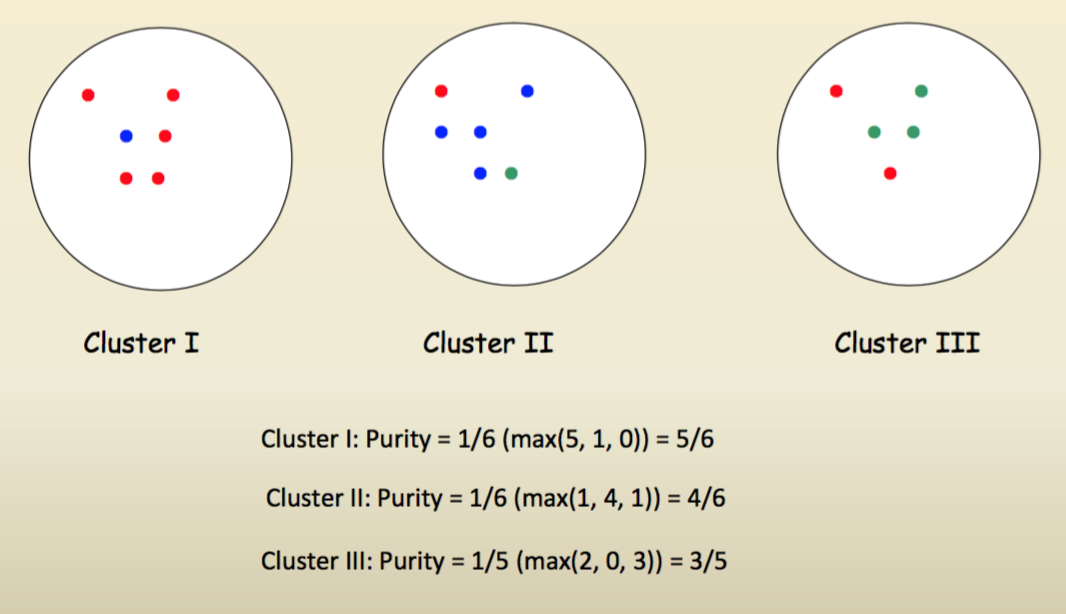
\includegraphics[width=\textwidth]{./notes/immagini/l17-purity.png}
\caption{Purity calcolata su 3 cluster}
\end{figure}

Nell'esempio il numero di cluster coincide con il numero di etichette ed è
una cosa voluta, ma il gioco funziona anche con un numero diverso di
cluster.

Questo perché le etichette note a priori vengono utilizzate solamente per valutare il clustering e non per effettuare l'apprendimento.

\subsubsection{Rand Index}\label{rand-index}

È una misura di similarità tra cluster, definita come il rapporto tra il
numero di elementi che hanno la stessa classe ground e si trovano nello
stesso cluster e con classi diverse in cluster diversi, sul numero
totale di elementi.

In altre parole è il rapporto tra il numero di elementi che si trovano nel cluster corretto e il numero totale di elementi.

\begin{figure}[htbp]
\centering
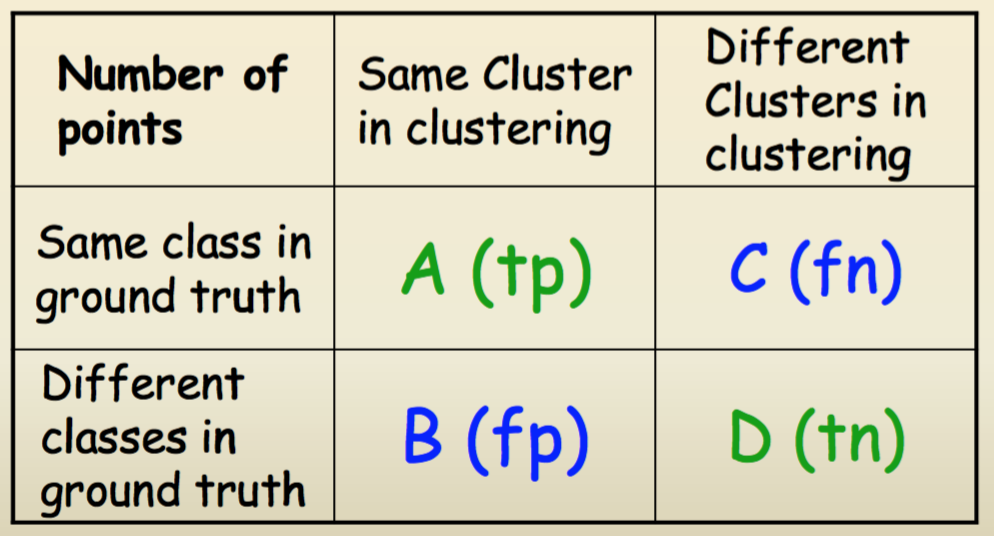
\includegraphics[width=0.6\textwidth]{./notes/immagini/l17-rand-index.png}
\caption{Elementi necessari per il Rand Index}
\end{figure}

Per calcolare il Rand Index, viene creata una tabella di contingenza, valutando per ogni coppia di
punti, se hanno etichette diverse e se sono nello stesso cluster.

Probabilmente, ma non ne sono sicuro, i numeri della tabella corrispondo
alle coppie che rispondo a quella categoria.

In questo modo ci si riconduce all'accuracy:

$$
RI =\frac{A + D}{A+B+C+D}
$$

Allo stesso modo si possono calcolare \textbf{precision} e
\textbf{recall} (§\ref{sec:pre-rec})

$$
P = \frac{A}{A+B} \qquad R = \frac{A}{A+C}
$$

\subsection{Algoritmi di Clustering}\label{algoritmi-di-clustering}

Ci sono due tipologie di algoritmi:

\begin{itemize}
\item
  \textbf{partitional}: che partono da un partizionamento casuale e
  cercano di migliorarlo iterativamente (K-means clustering, Model based
  clustering)
\item
  \textbf{hierarchical}: che vanno a definire un clustering come un
  albero in cui la radice contiene tutti gli esempi e man mano che si
  scende questi vengono partizionati. Si può usare un approccio
  \textbf{agglomerative} che costruisce l'albero in modo bottom-up
  (permettendo di fissare un numero di cluster), o \textbf{divisive} che
  funziona in top-down, applicando K-means sulla radice e poi
  ricorsivamente su ogni figlio, arrivando fino alla foglie che
  consistono in cluster di un solo elemento.
\end{itemize}

\subsection{K-means}\label{k-means}

Questo algoritmo appartiene alla categoria degli algoritmi di
partizionamento, ovvero vengono partizionati gli \emph{n} documenti in
\emph{K} cluster, cercando di trovare un partizionamento ottimo secondo
un determinato criterio.

Gli elementi da clusterizzare sono dei vettori con numeri reali e come
criterio di partizionamento si utilizza la distanza vettoriale tra gli
esempi e il centro del cluster.

Si cerca quindi di creare dei cluster che minimizzano il raggio della
iper-sfera che contiene gli esempi e che ha come centro $c$. (cluster \textbf{centroidi})

La formula da minimizzare è la seguente:

$$
\vec{\mu}(c) = \frac{1}{|c|}\sum_{\vec{x} \in c} \vec{x}
$$

\subsubsection{Algoritmo}\label{algoritmo}

\begin{enumerate}
\item
  Si posizionano K punti a caso nello spazio degli oggetti da
  clusterizzare, questi punti rappresentano i centroidi dei cluster.
\item
  Si assegna ogni oggetto al centroide più vicino.
\item
  Una volta completato l'assegnamento si ricalcola la posizione di tutti
  i centroidi utilizzano la media dei valori di tutti gli oggetti che
  sono finiti nel cluster.
\item
  Si ripetono i passi 2 e 3 finché non si spostano più i centrodi, ovvero finché non si raggiunge un punto fisso.
\end{enumerate}

L'iper-parametro $K$ dell'algoritmo è tipicamente soggetto a dei vincoli noti a priori oppure è da ottimizzare, ovvero trovare il numero \textit{corretto} di cluster in cui si dividono i dati.

\subsection{Approcci gerarchici agglomerativi}\label{approcci-gerarchici-agglormerativi}

\textbf{quelli divisi utilizzano ricorsivamente k-means}

Costruiscono un dendogramma a partire dagli oggetti, che vengono
agglomerati tra loro quando vengono trovati simili. Si ripete il
procedimento finché tutti gli oggetti non vengono agglomerati in un
unico cluster.

Si parte quindi da \textit{N} cluster, uno per ogni esempio e si agglomerano via
via finché non si ottiene un unico cluster.

Ad ogni iterazione l'algoritmo può essere interrotto per evitare di
ottenere un unico cluster.

Le linee verticale di un dendogramma rappresentano un cluster, mentre
quelle orizzontali rappresentano un punto di \textbf{merge} ovvero
quando la similarità di due cluster è tale che vengono uniti in un unico
cluster.

\begin{figure}[htbp]
\centering
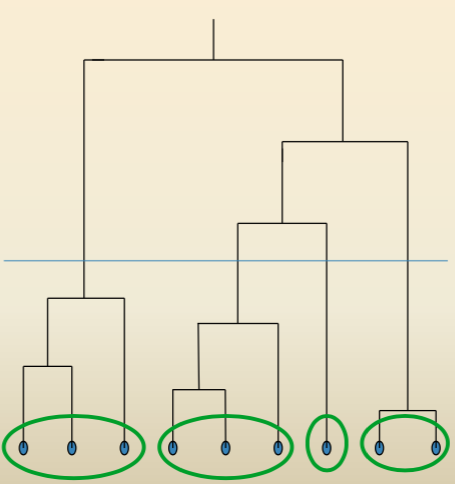
\includegraphics[width=.5\textwidth]{./notes/immagini/l17-clustering.png}
\caption{Esempio di un dendogramma}
\end{figure}

In base alla misura di similarità l'operazione può essere
\textbf{monotona} o meno, cioè se $s_1, \ldots, s_{k-1}$ sono
combinazioni di similarità associate a delle operazioni di merge, allora
$s_1 \geq s_2 \geq \ldots \geq s_{k-1}$

La non monotonicità, ovvero l'aumento della similarità in una serie di merge, contraddice l'assunzione fondamentale che cluster con pochi elementi sono più coerenti di cluster con tanti elementi\footnote{\url{http://nlp.stanford.edu/IR-book/html/htmledition/centroid-clustering-1.html}}.

\subsubsection{HAC - Hierarchical agglormerative
Clustering}\label{hac---hierarchical-agglormerative-clustering}

Prima viene creato un cluster per ogni esempio, dopodiché viene eseguito
via via il merge del \textbf{closest pair}, ovvero dei due cluster più
simili, fino a che non rimane un unico cluster. Lo storico dei merge
crea il dendogramma.

Come criteri di similarità tra i due cluster è possibile utilizzare:

\begin{itemize}
	\item la distanza euclidea: $||a-b||^2$, più è bassa, più simili sono i cluster
	\item la similarità coseno: $\frac{A \cdot B}{||A|| \cdot ||B||}$ che tende a 1 se i due esempi sono simili e a 0 se sono diversi.
	\item distanza di Manhattan: $\sum_i|a_i - b_i|$, più è bassa, più simili sono i cluster
\end{itemize}

Una volta scelta la misura di similarità, questa può essere calcolata per una coppia di cluster in vari modi:

\begin{itemize}
\item
  \textbf{single link}: viene calcolata la similiarità tra tutti gli elementi dei due cluster e viene scelto il valore massimo.
\item
  \textbf{complete link}: viene calcolata la similarità tra tutti gli elementi dei due cluster e viene scelto il valore minimo
\item
  \textbf{centroid link}: viene utilizzata la similarità tra i due centroidi dei due cluster
\item
  \textbf{average link}: viene calcolata la similarità tra tutti gli elementi dei due cluster e ne viene fatta la media.
\end{itemize}

Single, complete e average link garantiscono la monotonicità, mentre utilizzando centroid link alcune operazioni di merge potrebbero essere non monotone, ad esempio quando è necessario fare il merge di 3 cluster equidistanti tra loro.

Una volta calcolata la similarità tra tutti i cluster viene scelto il closest pair e viene fatto il merge.

\paragraph{Esempio - Distanza euclidea}

Scegliendo come misura la distanza euclidea, si ottiene che \textbf{minore è la distanza, più simili sono i cluster}. Pertanto i vari modi per calcolarle la similarità diventano:

\begin{itemize}
	\item
	\textbf{single link}: distanza tra i due punti più vicini dei due cluster
	\item
	\textbf{complete link}: distanza tra i due punti più lontani dei due cluster
	\item
	\textbf{centroid link}: distanza tra i centroidi dei due cluster
	\item
	\textbf{average link}: distanza media tra tutti i punti dei due cluster
\end{itemize}

\paragraph{Esempio - Similarità coseno}

Scegliendo come misura la similarità coseno, si ottiene che \textbf{maggiore è il valore, più simili sono i cluster}. Pertanto i vari modi per calcolarle la similarità diventano:

\begin{itemize}
	\item
	\textbf{single link}: similarità coseno tra i due punti più simili dei due cluster, ovvero che hanno similarità coseno più vicina ad 1.
	\item
	\textbf{complete link}: similarità cosento tra i due punti più diversi dei due cluster, ovvero che hanno similarità coseno più vicina a 0.
	\item
	\textbf{centroid link}: similarità coseno tra i due centroidi dei cluster
	\item
	\textbf{average link}: similarità media tra tutti gli elementi dei 
\end{itemize}

\begin{figure}[htbp]
\centering
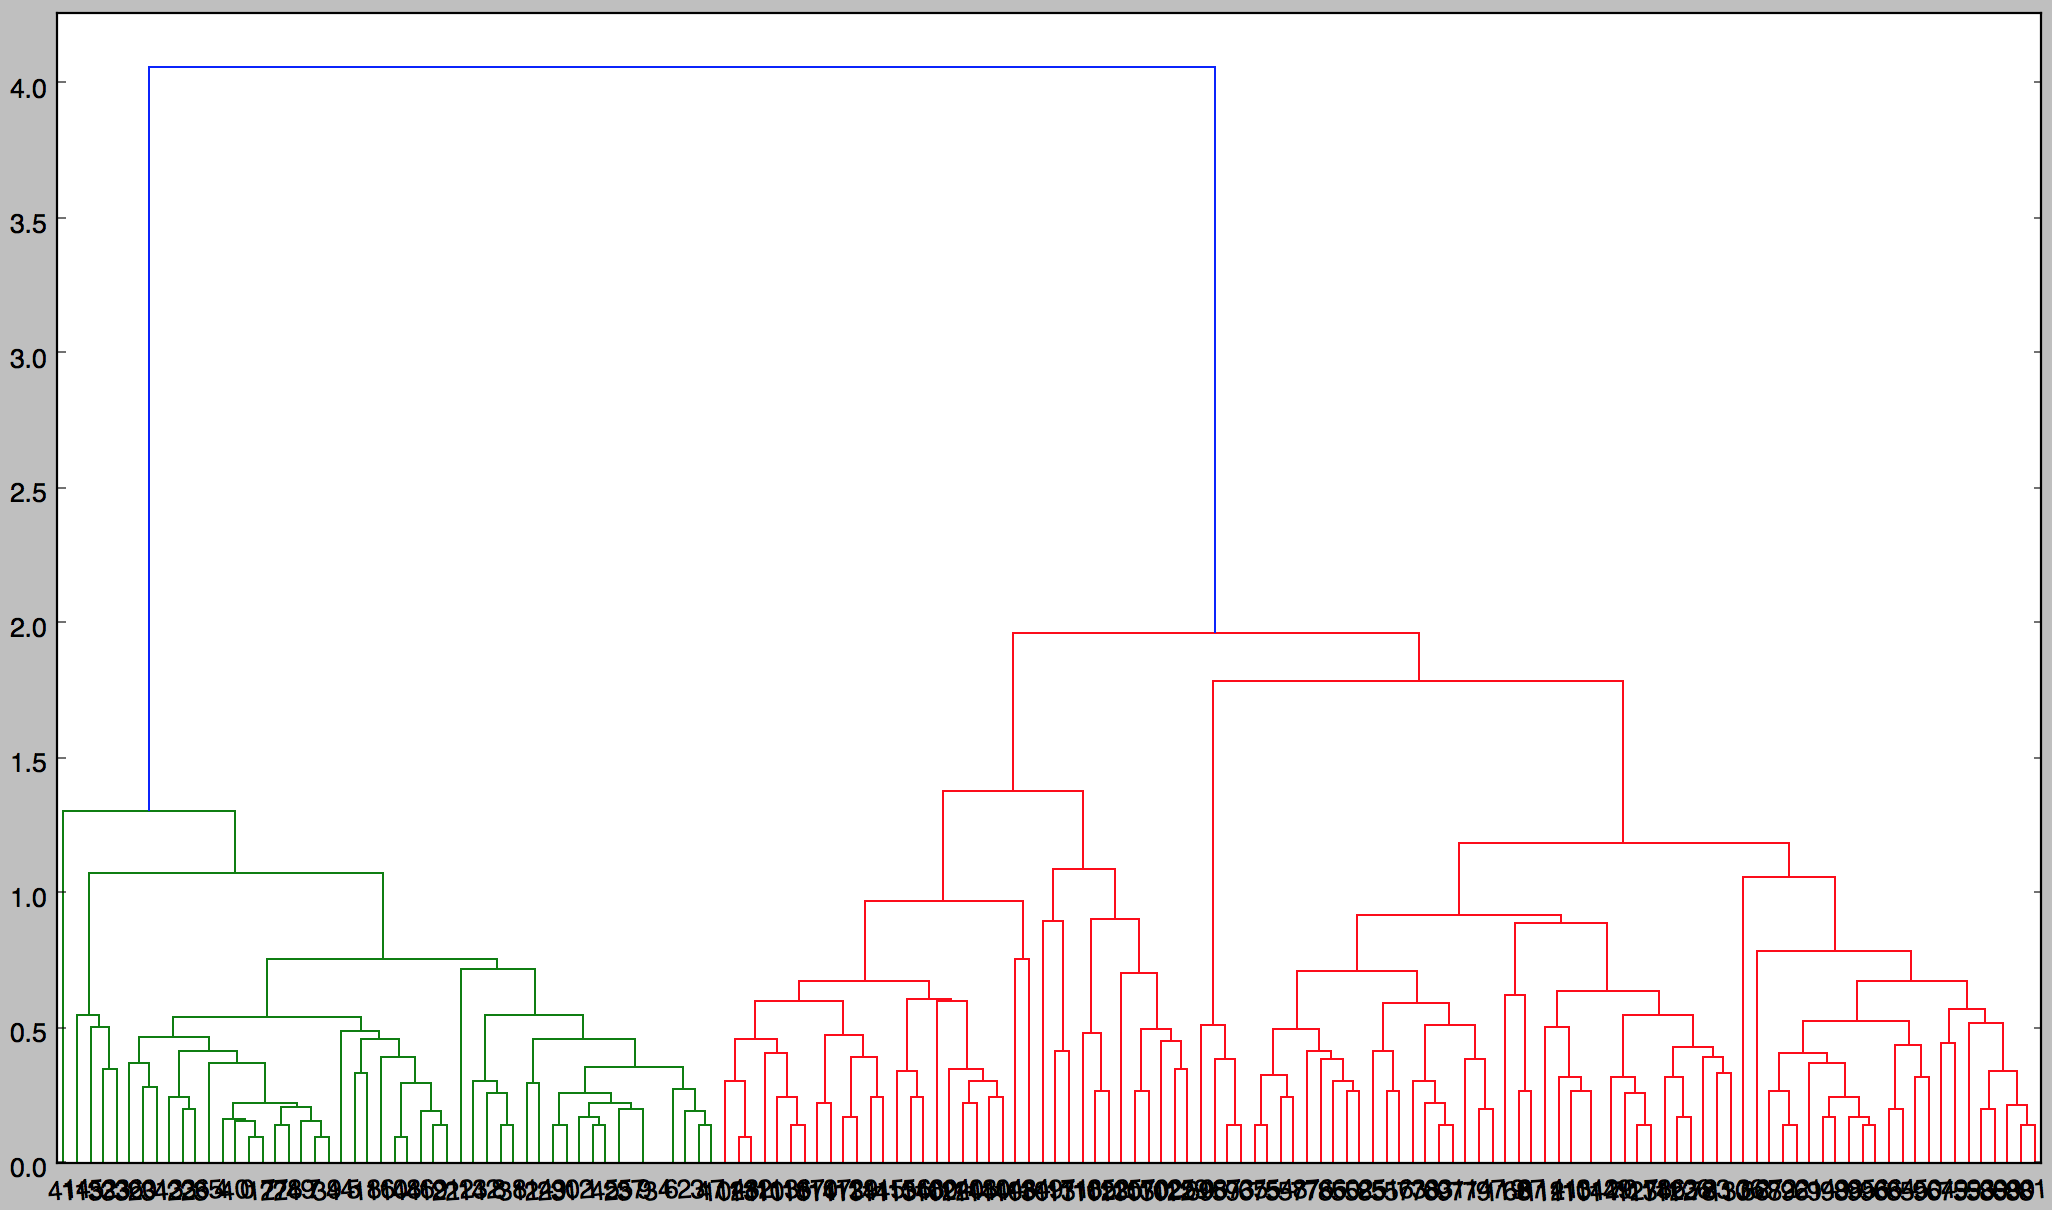
\includegraphics[width=\textwidth]{./notes/immagini/l17-dendogram-cluster.png}
\caption{Esempio di clustering ottenuto con HAC}
\end{figure}

Sia single link che complete link garantiscono la monotonia, tuttavia
con single link si tendono a creare dei cluster che sono delle
\emph{catene}, ovvero si ottengono dei dendogrammi sbilanciati, mentre
il complete link tende a dare dei cluster sferici e più compatti, se
però ci sono degli esempi \textbf{outliers}\todo{Da verificare}, ovvero che escono dalla
distribuzione.

Il centroid link è carino ma non garantisce la monotonia.

\begin{figure}[htbp]
\centering
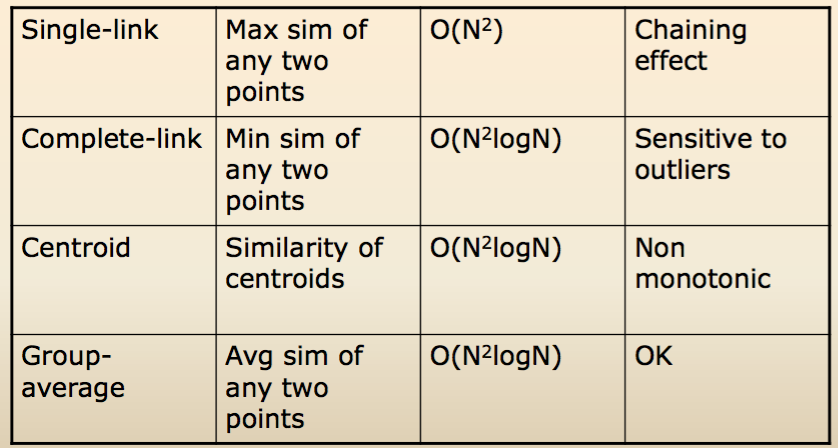
\includegraphics[width=\textwidth]{./notes/immagini/l17-riassunto.png}
\caption{Tabella riassuntiva, le complessità della tabella indicano quante operazioni servono per
	scegliere il closest pair}
\end{figure}

% !TEX encoding = UTF-8
% !TEX TS-program = pdflatex
% !TEX root = computabilità e algoritmi.tex
% !TEX spellcheck = it-IT
\chapter{Programmi generici - Lezione 18}

\section{Enumerazione dei programmi}

\textbf{Enumerazione delle funzioni calcolabili}: Un insieme \textit{X} è numerabile se esiste una funzione $ f : \mathbb{N} \rightarrow X $ suriettiva tale che $ \underbrace{f(0), f(1), f(2), \ldots}_{\mathbb{N}} $.


\subsection{Enumerazioni di supporto}
Per poter enumerare e quindi codificare dei programmi è necessario prima definire alcune funzioni biunivoche di supporto:

\begin{enumerate}
	\item $ \Pi : \mathbb{N}^2 \rightarrow \mathbb{N}$
	\item $ \nu : \mathbb{N}^3 \rightarrow \mathbb{N}$
	\item $ \tau : \bigcup\limits_{k \geq 1}\mathbb{N}^k \rightarrow \mathbb{N}$
\end{enumerate}

\subsubsection{$1. \: \Pi $}

Già osservata precedentemente, ovvero è la codifica delle coppie:

\begin{align*}
\Pi(x, y) &= 2^x(2y + 1) - 1\\
\Pi^{-1}(n) &= (\Pi_1(n), \Pi_2(n))
\end{align*}

\subsubsection{$2. \: \nu $}

$\nu $ può essere definita utilizzando $ \Pi $:

\begin{align*}
\nu(x_1, x_2, x_3) &= \Pi(\Pi(x_1,x_2), x_3) \\
\nu'(n) &= (v_1(n), v_2(n), v_3(n)) \\
\nu_1(n) &= \Pi_1(Pi_1(n))
\end{align*}

\subsubsection{$3. \: \tau $}

$ \tau $ può essere definita come $ (x_1, \ldots, x_k) \rightsquigarrow \prod\limits_{i=1}^{k} P_{i}^{x_i} -1$ ma questa funzione non è iniettiva:

\begin{align*}
(2,1) &= 2^2 \cdot 3^1 -1 \\
(2,1,0) &= 2^2 \cdot 3^1  \cdot 5^0 -1
\end{align*}

pertanto è necessario utilizzare

$$
\tau(x_1, \ldots, x_k) \rightsquigarrow \prod\limits_{i=1}^{k-1} P_{i}^{x_i} \cdot P_{k}^{x_{k+1}} - 2
$$

Per decodificare un numero \textit{n} è necessario prima calcolare la lunghezza della decodifica:

$$
l(n) = \max k.P_k \text{ divide } (n+2) \text{ con } k \leq n
$$

Anche se si tratta di una massimizzazione illimitata è possibile dimostrare che è calcolabile sfruttando la minimalizzazione illimitata, e quindi $ l(n) \in \mathcal{PR} $.

$$
a(n,i) = \begin{cases}
(n+2)_i &\text{ se } i < l(n)\\
(n+2)_i -1 &\text{ se } i = l(n)
\end{cases}
$$

l'inversa di $ \tau $ può essere definita come:

$$
\tau^{-1}(n) = \Big(a\big(n,1\big), a\big(n,2\big), \ldots, a\big(n,l(n)\big)\Big)
$$

\subsection{Enumerazione dei programmi}

Grazie alle funzioni precedentemente definite è possibile definire delle codifiche biunivoche che permettono di codificare con un numero sia una singola istruzione URM, sia un qualsiasi programma URM in $ \mathcal{P} $.

$$
\beta : \text{Ist URM} \rightarrow \mathbb{N} \quad \text{e} \quad \gamma : \mathcal{P} \rightarrow \mathbb{N}
$$

\subsubsection{$ \beta : \text{Ist URM} \rightarrow \mathbb{N} $}

\begin{align*}
Z(n) &\rightarrow 4\cdot(n-1) \\
S(n) &\rightarrow 4\cdot(n-1)+1 \\ 
T(m,n) &\rightarrow 4\cdot\big(\Pi(m-1,n-1)\big)+2 \\
J(m,n,t) &\rightarrow 4\cdot\big(\tau(m-1,n-1,t-1)\big)+3
\end{align*}

I vari $ -1 $ servono perché i registri URM partono da 1, mentre la codifica deve partire da 0, altrimenti non sarebbe biunivoca.

La moltiplicazione per 4 serve per ``\textit{fare spazio}'' nella codifica in modo da continuare ad avere una funzione biunivoca. Allo stesso scopo servono anche le somme finali.

per fare l'inversa di $ \beta $ basta calcolare $ r = rm(4,n) $ e $ q = qt(4,n) $:

$$
\beta^{-1} \begin{cases}
Z(q+1) &\text{ se } r=0 \\
S(q+1) &\text{ se } r=1 \\
T\big(\Pi_1(q)+1, \Pi_2(q)+1\big) &\text{ se } r=2 \\
J\big(a(q,1)+1,a(q,2)+1,a(q,3)+1\big)&\text{ se } r=3
\end{cases}
$$
\todo{Verificare J}

In questo modo si ha una codifica per le istruzioni che permette di trasformare una sequenza di istruzioni in una sequenza di numeri

\subsubsection{$ \gamma : \mathcal{P} \rightarrow \mathbb{N} $}

$$
\gamma(P) = \tau\big(\beta(I_1), \beta(I_2), \ldots\big)
$$

inversa con:

$$
\gamma^{-1}(n) = \tau^{-1}(n) = \Big(a\big(n,1\big), a\big(n,2\big), \ldots, a\big(n,l(n)\big)\Big)
$$

\section{Verso il programma 33 e la sua funzione}

Con quanto a disposizione si può parlare del programma 33, ottenuto decodificando il numero 33.

Prima di continuare serve della notazione aggiuntiva:

Dato $ P \in \mathcal{P} $, $ \gamma(P) $ indica il codice di \textit{P} e prende il nome di \textbf{G\"odel number}.

Dato \textit{n}, $ \gamma^{-1}(n) $ rappresenta il programma codificato nel numero \textit{n}, tale programma viene indicato con $ P_n $.

Un esempio è dato da:
\begin{lstlisting}[language=URM]
P:
T(1,2) 		--> 4Pi(1-1, 2-1) +2= 10
S(2)		  --> 4(2-1) = 4
T(2,1)   	--> 4Pi(2-1,1-1) +2= 6
\end{lstlisting}

\begin{align*}
\gamma(P) &= \tau(10,4,6)\\
&= 2^10 + 3^4 + 5^{6+1} -2\\
&= 19.439.999.998
\end{align*}

\begin{lstlisting}[language=URM]
P':
S(1)		--> 2
\end{lstlisting}

$$
\gamma(P’) = \tau(P) = 2
$$

I numeri $ 19.439.999.998 $ e $ 2 $ rappresentano due programmi che calcolano la stessa funzione successore.

Si può fare anche l'operazione inversa:

\begin{verbatim}
100
gamma^{-1}(100)  100+2
= 2^1 + 3^1 + 17 ^1
P1^1 P2^1 P3^0 P4^0 P5^0 P6^0 P7^1
1 -> S(1)
1 -> S(1)
0 -> Z(1)
0 -> Z(1)
0 -> Z(1)
0 -> Z(1)
1 -> S(1)
\end{verbatim}

Il numero $ 100 $ rappresenta quindi il programma che calcola la constante 1.

Dal momento che è possibile codificare i programmi in un numero, viene indotta anche un'enumerazione sulle funzioni calcolate da questi programmi:

Fissata $ \gamma : \mathcal{P} \rightarrow \mathbb{N} $, si ha:

$$
\phi_{n}^{(k)} = f_{P_n}^{(k)}
$$

ovvero $ \phi_{n}^{(k)} $ è la funzione di \textit{k} argomenti calcolata da $ P_n = \gamma^{-1}(n) $.
Per questa funzione è possibile definire anche 

$$
W_{n}^{(k)} = dom(\phi_{n}^{(k)}) \subseteq \mathbb{N}^k = \{\vec{x}\: | \: \vec{x} \in \mathbb{N}^k \text{ tale che } \phi_{n}^{(k)}(\vec{x}) \downarrow\}
$$

$$
E_{n}^{(k)} = cod(\phi_{n}^{(k)}) = \{y\:|\: \exists\vec{x} \: \phi_{n}^{(k)}(\vec{x}) = y  \}
$$

Ad esempio:

\begin{align*}
P: S(1) &\rightarrow \gamma(P) = 2 \\
\phi_{2}^{(1)}(x) &= x+1 \\
W_{2}^{(1)} &= \mathbb{N} \\
E_{2}^{(1)} &= \mathbb{N} - \{0\} \\
\end{align*}

Inoltre, si può definire una sorta di funzione di ordine superiore che, una volta fissato un $ k \geq 1$, associa un numero $ \mathbb{N} $ ad una funzione in $ \mathcal{C}^{(k)} : n \rightarrow  \phi_{n}^{(k)}$. Questa funzione è suriettiva perché data $ f \in \mathcal{C}^{(k)} $ esiste un programma \textit{P} che calcola $ f = f_{P}^{(k)} = \phi_{\gamma(P)}^{(k)} $ .
Questa funzioni non è iniettiva perché una stessa funzione può essere calcolata da più programmi.

Quindi 

$$
|\: \mathcal{C}^{(k)}\:| =  |\: \mathbb{N}\:| \leq |\: \mathcal{C}\:| = |\: \bigcup\limits_{k \geq 1} \mathcal{C}^{(k)} \:| = |\: \mathbb{N}\: |
$$
\todo{Verificare}

ovvero esistono delle funzioni che non sono calcolabili.














% !TEX encoding = UTF-8
% !TEX program = pdflatex
% !TEX root = InformationRetrieval.tex
% !TEX spellcheck = it-IT

% 15 Dicembre 2016

\chapter{Anatomia e performance di un sistema di IR}

Nel nostro progetto noi non stiamo misurando lo stemmer di per se, ma stiamo misurando quanto lo stemmer migliora i risultati del sistema rispetto all'esecuzione senza stemming.

Si ha però che il sistema è composto da molti blocchi: tokenizzatore, stoplist, stemmer, modello e quindi non è semplice valutare il singolo componente, perché le prestazioni del sistema possono essere influenzate dagli altri componenti o dai parametri con i quali sono configurati.

Le misure nell'IR sono quindi misure end-to-end che considerano la totalità del sistema. Per valutare un singolo componente stabilisco quindi una pipeline di componenti e vario solamente quello che voglio misurare.

\section{Grid@CLEF}

L'idea è quindi quella di sviluppare un sistema di testing che funzioni con più lingue (MLIA: Multilingual Information Access) per capire come migliorare le performance dei singoli componenti.

Questo si può ottenere conducendo una serie di griglie di esperimenti, sistematici e ripetibili, su diversi linguaggi e con diversi componenti, effettuando uno sforzo comunitario per valutare sia i singoli componenti che la loro interazione con gli altri.

Per implementare questo sistema è stata sviluppata una soluzione asincrona, basata su una produzione di dump intermedi XML, da scambiare tra i vari gruppi di ricerca. Ad esempio quelli che lavoro su un tokenizzatore, possono fornire i loro output ad un gruppo di ricerca che lavora agli stemmer per il tedesco.
Ci sono stati dei problemi implementativi però qualcosa si è riuscito a fare.

\begin{figure}[htbp]
	\centering
	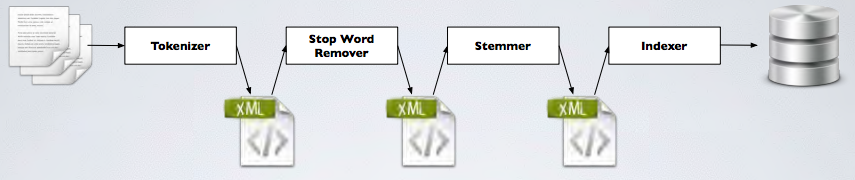
\includegraphics[width=0.5\textwidth]{images/l20-fig-1}
	\caption{Utilizzo dei file XML condivisi dai vari gruppi di ricerca.}
\end{figure} 

Mancava però una metodologia per analizzare i risultati di questi esperimenti.

Nel 2015 alla conferenza SIGIR-RIGOR si è iniziato ad invitare gli sviluppatori di motori open-source a fornire delle baseline di valutazione per i loro sistemi in un ambiente comune.
L'idea era quella di creare questo ambiente comune dove chi volesse valutare una nuova tecnica fosse in grado di utilizzare un motore di ricerca già esistente per il confronto/implementazione. Questo ambiente doveva essere anche aperto in modo che fosse possibile capire se durante i test i sistemi utilizzati fossero stati configurati nella maniera corretta.
Si voleva quindi fornire una baseline da utilizzare come riferimento per i nuovi metodi e allo stesso modo la baseline era in un certo senso certificata perché era nota a tutti e quindi se qualcuno ha presentato dei nuovi modelli comparandoli con una baseline è possibile capire se la baseline di riferimento è sufficientemente buona e quindi i risultati sono concreti, oppure se è stata scelta una baseline pessima e quindi i risultati sembrano migliori di quanto lo sono in realtà.

Ma anche in questo caso mancava una sistema di analisi dei dati.

\begin{figure}[htbp]
	\centering
	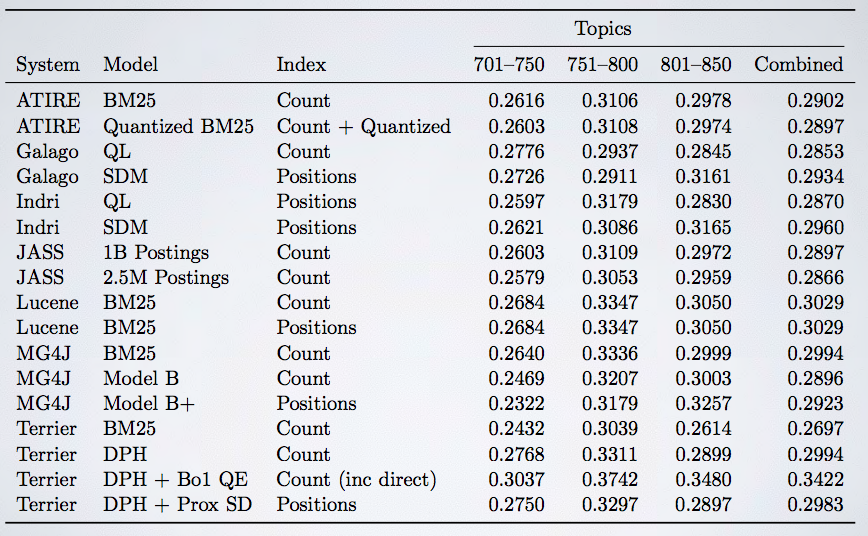
\includegraphics[width=0.5\textwidth]{images/l20-fig-2}
	\caption{Alcuni risultati (Mean Avarage Precision) ottenuti su TREC con il metodo proposto da RIGOR.}
\end{figure} 

\section{Valutazione delle performance - General Linear Mixed Model}

Posso combinare i dati dell'esecuzione dei vari sistemi della griglia in una matrice in cui le righe rappresentano i topic e le colonne sono i vari sistemi. Il valore delle cella è dato dall'average precision del sistema sul dato topic.
La matrice poi può essere plottata in una heat map (figura \ref{fig:heatmap}), in modo che sia più comprensibile.

\begin{figure}[htbp]
	\centering
	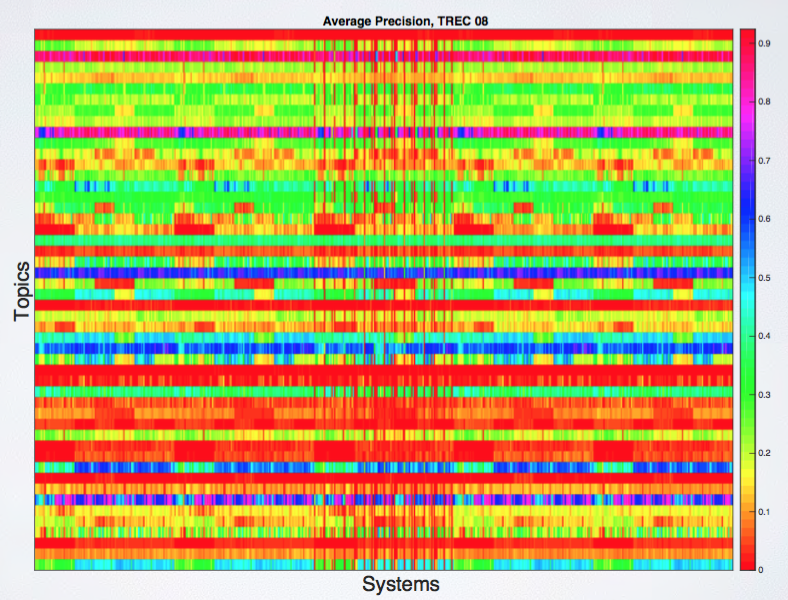
\includegraphics[width=0.5\textwidth]{images/l20-fig-3}
	\caption{Rappresentazione mediante heatmap della matrice. Nelle righe ci sono i topic mentre nelle colonne i vari sistemi.}\label{fig:heatmap}
\end{figure} 

Dalla figura \ref{fig:heatmap} si può notare che la variazione nella precisione è maggiore al variare dei topic, ovvero sistemi diversi tendono ad avere prestazioni simili sullo stesso topic.
Questo perché le performance del sistema dipendo sia dalla struttura del sistema, che dalla difficoltà del topic.

Pertanto si è pensato di modellare questa variazione della precisione con un \textbf{General Linear Mixed Model}, il quale spiega la variazione della variabile dipendente $Y$ nei termini della variabile indipendente, in questo caso il modello e di una varianza residua non controllata, che modella gli errori.

La scelta di questo modello è stata fatta perché gestisce variabili sia continue che categoriche (\textit{general}) che sono tra loro in combinazione lineare (\textit{linear}) e che dipendono da fattori sia fissi che casuali (\textit{mixed}).

Nel nostro caso lavoriamo con variabili di tipo categorico, perché anche se la MAP è un valore continuo a noi interessa la combinazione topic-sistema che è discreta.

Dobbiamo poi tener conto che questo deve poi essere applicato a degli esperimenti che possono essere considerati come indipendenti o ripetuti. Negli esperimenti \textbf{indipendenti} ogni soggetto viene provato con un fattore, mentre in quelli \textbf{ripetuti} su ogni soggetto vengono provati su tutti i fattori. Noi siamo nel caso ripetuto perché lo stesso topic viene provato su tutti i sistemi a disposizione.

Gli esperimenti possono poi essere \textbf{fattoriali} se tutti i fattori sono provati da tutti i soggetti oppure \textbf{nested} se per ogni soggetto viene provato solo un sotto-insieme delle possibili combinazioni di fattori. Noi siamo nel caso fattoriale.

I nostri modelli sono quindi a fattori fissi perché i topic sono finiti, con misure ripetute e combinazioni fattoriali.

Possiamo quindi modellare l'average precision con:

$$
Y_{ij} = \underbrace{\mu_{\cdot \cdot} + \tau_i + \alpha_j}_{Modello} + \underbrace{\epsilon_{ij}}_{Errore}
$$

\noindent dove:
\begin{itemize}
	\item $Y_{ij}$ è la variabile dipendente che voglio andare a stimare, ovvero nel nostro caso, l'average precision.
	\item $\mu_{\cdot\cdot}$ è la media di tutte le average precision (generale) che funziona come valore base ($\beta_0$, il valore dell'intercetta).
	\item $\tau_i$ è l'effetto del topic $i$.
	\item $\alpha_j$ è l'effetto del sistema $j$.
	\item $\epsilon_{ij}$ l'errore, ovvero tutto quello che il nostro modello non considera.
\end{itemize}

Il tutto poi può essere raccolto nella seguente tabella.

\begin{table}[htbp]
	\centering
	\begin{tabular}{llllll}
		\cline{2-5}
		\multicolumn{1}{l|}{}  & \multicolumn{1}{l|}{$ A_1 $} & \multicolumn{1}{l|}{$ A_2 $} & \multicolumn{1}{l|}{$ \ldots $} & \multicolumn{1}{l|}{$ A_p $} &  \\ \cline{1-5}
		\multicolumn{1}{|l|}{$ T'_1 $} & \multicolumn{1}{l|}{$ Y_{11} $} & \multicolumn{1}{l|}{$ Y_{12} $} & \multicolumn{1}{l|}{$ \ldots $} & \multicolumn{1}{l|}{$ Y_{1p} $} & $\mu_{1\cdot}$ \\ \cline{1-5}
		\multicolumn{1}{|l|}{$ T'_2 $} & \multicolumn{1}{l|}{$ Y_{21} $} & \multicolumn{1}{l|}{$ Y_{22} $} & \multicolumn{1}{l|}{$ \ldots $} & \multicolumn{1}{l|}{$ Y_{2p} $} & $\mu_{2\cdot}$ \\ \cline{1-5}
		\multicolumn{1}{|l|}{$\vdots$} & \multicolumn{1}{l|}{$\vdots$} 	 & \multicolumn{1}{l|}{$\vdots$}   & \multicolumn{1}{l|}{$ Y_{ij}$}  & \multicolumn{1}{l|}{$\vdots$}   & $\mu_{i\cdot}$ \\ \cline{1-5}
		\multicolumn{1}{|l|}{$ T'_n $} & \multicolumn{1}{l|}{$ Y_{n1} $} & \multicolumn{1}{l|}{$ Y_{n2} $} & \multicolumn{1}{l|}{$ \ldots $} & \multicolumn{1}{l|}{$ Y_{np} $} & $\mu_{n\cdot}$ \\ \cline{1-5}
		                               &      $\mu_{\cdot1}$             & $\mu_{\cdot2}$                  & $\mu_{\cdot j}$                 &   $\mu_{\cdot p}$               & $\mu_{\cdot\cdot}$
	\end{tabular}
	\caption{La matrice precedentemente osservata, rappresentata secondo il nostro modello. Le righe rappresentano i soggetti degli esperimenti ripetuti, nel nostro caso i topics, mentre le colonne rappresentano i fattori, ovvero i sistemi di IR.}
	\label{my-label}
\end{table}

Ovviamente questo è solamente il modello, restano ancora da stimare i vari parametri del modello, per fare la validazione del modello.

\subsection{Stima dei parametri del modello}

Siamo quindi in una situazione nella quale riusciamo ad osservare la variabile dipendente $Y_{ij}$ con i nostri esperimenti e dobbiamo stimare i parametri del nostro modello.

Si ha quindi che la media totale $\mu_{\cdot \cdot}$ può essere stimata con la media aritmetica di tutte le celle della matrice, ovvero:

$$
\hat{\mu}_{\cdot \cdot} = \frac{1}{pn}\sum\limits_{j=1}^{p}\sum\limits_{i=1}^{n} Y_{ij}
$$

Per stimare i vari effetti dei singoli topic e dei singoli sistemi posso utilizzare le medie marginali, rimuovendo l'andamento generale dato da $\hat{\mu}_{\cdot \cdot}$.
Quindi:

\begin{align*}
	\hat{\mu}_{i\cdot} & \frac{1}{p}\sum\limits_{j=1}^{p} Y_{ij} \qquad \hat{\tau} = \hat{\mu}_{i\cdot} - \hat{\mu}_{\cdot\cdot} \\
	\hat{\mu}_{\cdot j} &= \frac{1}{n}\sum\limits_{i=1}^{n} Y_{ij} \qquad \hat{\alpha} = \hat{\mu}_{\cdot j} - \hat{\mu}_{\cdot\cdot}
\end{align*}

Possiamo quindi utilizzare il nostro modello stimato per effettuare la stima dell'average precision:

$$
\hat{Y}_{ij} = \hat{\mu}_{\cdot\cdot} + \hat{\tau}_i + \hat{\alpha}_j = \hat{\mu}_{i\cdot} + \hat{\mu}_{\cdot j} - \hat{\mu}_{\cdot\cdot}
$$

con il quale possono andare ad effettuare anche una stima dell'errore commesso dal modello:

$$
\hat{\epsilon}_{ij} = Y_{ij} - \hat{Y}_{ij} = Y_{ij} - (\hat{\mu}_{i\cdot} + \hat{\mu}_{\cdot j} - \hat{\mu}_{\cdot\cdot})
$$









% !TEX encoding = UTF-8
% !TEX TS-program = pdflatex
% !TEX root = computabilità e algoritmi.tex
% !TEX spellcheck = it-IT

\chapter{Esercizi in preparazione al parziale}


\section{Teorema SMN}

\subsection{Esercizio 1}

Dimostrare che esiste $ S : \mathbb{N} \rightarrow \mathbb{N}$ tale che $|\: W_{S(x)}\:|  = 2 x$ e $ |\: E_{S(x)}\:| =x $

\subsubsection{Soluzione}

Si cerca una funzione $ f(x,y) $ che con $ x $ fissato abbia esattamente le caratteristiche richieste, ci pensa il teorema SMN a fare il resto.

\begin{align*}
f(x,y) &= \begin{cases}
y \dotminus x, &\text{ se } y < 2x \\
\uparrow, &\text{altrimenti}
\end{cases} \\
 &= y\dotminus x + \underbrace{\mu z. y +1 -2x}_{\text{fa divergere se } y \geq 2x}
\end{align*}

Questa funzione è calcolabile e quindi per il teorema SMN esiste $ S : \mathbb{N} \rightarrow \mathbb{N} $ tale che 

$$
\phi_{S(x)}(y) = f(x,y)
$$

e per costruzione $W_{S(x)} = [0,2x-1]$ e $ E_{S(x)} = [0,x-1] $.

\section{Calcolabilità delle funzioni}

\subsection{Esercizio 1}

Dimostrare che 

$$
f(x) = \begin{cases}
\phi_x(x) &\text{se} \phi_x(x)\downarrow \\
0 &\text{altrimenti}
\end{cases}
$$

non è calcolabile.

\subsubsection{Soluzione}

Non si può usare il \textit{trick} della diagonale, perché la funzione deve essere proprio uguale alla diagonale.

$$ h(x) = f(x)+1 = \begin{cases}
\phi_x(x)  + 1 &\text{se} \phi_x(x)\downarrow \\
1 &\text{altrimenti}
\end{cases}
 $$

Così facendo $ h \neq \phi_x(x) \forall x $ e pertanto non è calcolabile.

Ma $ h $ è il successore di $ f $, quindi $ f $ non può essere calcolabile, perché se così non fosse $ h(x) = f(x) +1 $ sarebbe calcolabile per composizione di funzioni calcolabili.ò

Da notare che questa cosa non vale in se e solo se:

$$ h(x) = f(x) +1 \text{ non calcolabile }\Rightarrow f(x)  \text{ non calcolabile } $$

ma \textbf{NON \`{E} VERO}

$$ f(x) \text{ non calcolabile } \Rightarrow f(x) = h(x) +1 \text{ non calcolabile }$$
%------------

\subsection{Esercizio 2}

Sia $ \mathbb{P} $ l'insieme dei numeri pari, dimostrare che la funzione caratteristica è primitiva ricorsiva.

$$
\mathcal{X}_\mathbb{P} = \begin{cases}
1 &\text{ se $ x $ è pari} \\
0 &\text{ altrimenti}
\end{cases}
$$

\subsubsection{Soluzione}

\begin{align*}
\mathcal{X}_\mathbb{P}(0) &= 1
\mathcal{X}_\mathbb{P}(x+1) &= \overline{sg}\big(\mathcal{X}_\mathbb{P}(x)\big)
\end{align*}

Dal momento che in un esercizio non sappiamo dell'esistenza del segno negato è necessario andare a mostrare che anche quella funzione è primitiva ricorsiva:

\begin{align*}
 \overline{sg}(0) &= 1 \\
  \overline{sg}(x+1) &= 0
\end{align*}


\subsection{Esercizio 3}

Dimostrare che la funzione $ half(x) = \lfloor\frac{x}{2}\rfloor $ è primitiva ricorsiva.

\subsubsection{Soluzione}

\begin{align*}
half(0) &= 0 \\
half(x+1) &= half(x) + rm_2(x)
\end{align*}

come prima bisogna dimostrare che $ rm_2 $ è ricorsiva primitiva

\begin{align*}
rm_2(x) &= 0
rm_2(x+1) &= \overline{sg}(rm_2(x))
\end{align*}

ma anche $ \overleftarrow{sg} $ è in $ \mathcal{PR} $

\begin{align*}
\overline{sg}(0) &= 1 \\
\overline{sg}(x+1) &= 0
\end{align*}

\section{Macchina URM}

\subsection{Esercizio 1}

Consideriamo la macchina $ \text{URM}^- $ che al posto dell'istruzione successore ha quella che effettua il predecessore.
Come sono in relazione le due classi? 

Ovvero:
 $$\mathcal{C}^- \text{ ? } \mathcal{C}$$
 
 \subsubsection{Soluzione}
 
 \`{E} chiaro che  $\mathcal{C}^- \subseteq \mathcal{C}$ perché la funzione predecessore può essere sostituita da un programma che calcola il predecessore.
 
 Per vedere \textbf{se}  $\mathcal{C}^- \supseteq \mathcal{C}$ bisogna provare a simulare il successore con un programma per la macchina $ \text{URM}^- $.

Ma dato un $ P \in \text{URM}^- $ qualsiasi $ P(\vec{x}) $ dopo $ n $ passi, $ \forall n $, tutti i registri $ r_i \leq \max x_i$.

Se $ n = 0 $ è ovvio perché i registri non cambiano.

Se $ n \rightarrow n+1 $, l'istruzione aggiunta può essere:
\begin{itemize}
	\item precessore ma il valore non aumenta
	\item zero azzera un registro
	\item il trasferimento non incrementa i valori
\end{itemize}

Dal momento che i registri di un programma in $ \text{URM}^- $ non aumentano mai, non è possibile implementare la funzione successore, quindi \textbf{non vale} la relazione $\mathcal{C}^- \supseteq \mathcal{C}$.


\subsection{Esercizio 2}
$ \text{URM}^S$ che non ha \texttt{S(n)} e \texttt{J(m,n,t)} ma ha \texttt{JS(m,n,t)} che prima fa il test e poi incrementa il registro $ m $.

\subsubsection{Soluzione}

$\mathcal{C}^S \subseteq \mathcal{C}$ perché un programma URM riesce ad emulare l'istruzione \texttt{JS}.

$\mathcal{C}^S \supseteq \mathcal{C}$ non vale, perché un programma $ \text{URM}^S$ non riesce a calcolare la funzione successore.


\section{Diagonalizzazione}

\subsection{Esercizio 1}

$ F_0 = \{f \: | \: \text{cod}(f) \subseteq \{0\} \text{ e parziali}\}$ è numerabile?

\subsubsection{Soluzione}

L'unica differenza tra queste funzioni è data dai domini che sono tanti quanti i numeri naturali.

Suppongo per assurdo che $ F_0 $ sia enumerabile, allora:

\begin{verbatim}
		f0	f1 f2
0      0   0   0
1      0   0
2
\end{verbatim}

considerando la diagonale, posso definire

$$
f(x) = \begin{cases}
0 &\text{se } f_x(x)\uparrow \\
\uparrow &\text{se } f_x(x)=0
\end{cases}
$$

$ f $ dovrebbe appartenere a $ F_0 $ ma per costruzione non compare nella enumerazione, quindi $ F_0 $ non è enumerabile.

\subsection{Esercizio 2}

$ f : \mathbb{N} \rightarrow \mathbb{N} $ totale e decrescente se $ \forall x,y \: x \leq y \Rightarrow f(y) \leq f(x) $.

$ F_d = \{ f : \mathbb{N} \rightarrow \mathbb{N} \: \ \: f \text{ totale e descrescente e } \text{cod}(f) \subseteq \{0,1\} \} $ è numerabile?

\subsubsection{Soluzione}

Le funzioni dell'insieme possono essere o costanti uguali a 0 o 1, oppure uguali a 1 fino ad un certo valore per poi diventare costanti a 0.

$$ \forall f \in F_d \: n(f)  = \text{sup}(\{x \: | \: f(x) = 1\})$$

$ n(f) $ è il punto in cui cambia il valore della funzione e caratterizza $ f $, ovvero

$$
\forall f_1, f_2 \in F_d \: n(f_1) = n(f_2) \Rightarrow f_1 = f_2
$$

quindi $ n : F_d \rightarrow \mathbb{N} \cup \{\infty\} $ è una funzione iniettiva e suriettiva, pertanto $ |\: F_d \:| = |\: \mathbb{N} \cup \{ \infty \} \:| $, ovvero $ F_d $ è numerabile.


\subsection{Esercizio 3}

Trovare $ f : \mathbb{N} \rightarrow \mathbb{N} $ totale e non calcolabile tale che $ f(x)  =x $ per infiniti $ x $.

\subsubsection{Soluzione}

$$
f(x) = \begin{cases}
x, &\text{ se $ x $ è pari} \\
\phi_{\frac{x-1}{2}}(x) +1, &\text{ se } \phi_{\frac{x-1}{2}}(x) \downarrow \\
0, &\text{ se } \phi_{\frac{x-1}{2}}(x) \uparrow 
\end{cases}
$$

\subsection{Esercizio 4}

Trovare una funzione $ f $ crescente, totale e non calcolabile.

\subsubsection{Soluzione}

$$
h(x) = \begin{cases}
\phi_x(x)+1, &\text{ se }\phi_x(x)\downarrow \\
0, &\text{ se } \phi_x(x) \uparrow
\end{cases}
$$

$ h $ è non calcolabile perché è definita sulla diagonale distorta.

$$
f(x) = \sum\limits_{y \leq x} h(y)
$$

Così definita $ f $ è:
\begin{itemize}
	\item totale
	\item crescente: $ f(x+1) = f(x) + h(x+1) \geq f(x) $
	\item $ \forall x $ se $ \phi_x(x) \downarrow \: f(x) = \sum\limits_{y \leq x} h(y) \geq h(x) = \phi_x(x) +1 \neq \phi_x(x) $ e se $ \phi_x(x) \uparrow $, $ h(x) = 0 \neq \phi_x(x) $, ovvero $ f $ non è calcolabile.
\end{itemize}

\subsection{Esercizio 5}

Può esistere $ f : \mathbb{N} \rightarrow \mathbb{N} $ non calcolabile tale che $ \forall g : \mathbb{N} \rightarrow \mathbb{N} $ non calcolabile $ f+g  $ è calcolabile?

$$
(f+g)(x) = f(x) + g(x)
$$

\subsubsection{Soluzione}

Non può esistere, perché per assurdo, sia $ f $ una funzione tale che $ (f+f) $ è calcolabile:

\begin{align*}
h(x) &= f(x) + f(x) \\
		&= 2 f(x)
\end{align*}

$h(x)$ è quindi calcolabile, però utilizzando questa funzione si può definire $ f(x) = qt(2, h(x)) $, dimostrando la calcolabilità di $ f $ che per ipotesi non è calcolabile.



% !TEX encoding = UTF-8
% !TEX program = pdflatex
% !TEX root = InformationRetrieval.tex
% !TEX spellcheck = it-IT

\section{Search Engine Optimization}

Il linguaggio HTML non è stato pensato per i motori di ricerca e per farci reperimento dell'informazione. Tutto è iniziato per trovare un modo di rappresentare dei documenti che funzionasse anche per non informatici.

\subsection{Ranking delle pagine}

Il \textbf{ranking statico} viene definito nel momento dell'indicizzazione effettuando l'analisi del contenuto e dei link presenti nella pagina web.

Questo dipende dall'uso dei link e dalla struttura della pagina, la quale deve riflettere la qualità, l'autorevolezza e la popolarità di una pagina web. 
Migliore è la qualità della pagina, maggiore è il rank statico calcolato dal motore per la pagina.

Da notare che se un motore di ricerca fornisce tra i primi risultati una pagina autorevole non implica che è un motore che funziona bene.

Il \textbf{ranking dinamico} viene calcolato combinando la query con il ranking statico delle pagine. Vengono quindi presi in considerazione alcuni fattori che dipendono dalla query come la presenza dei termini e le loro prossimità.
Le modalità di ranking statico e dinamico variano da motore a motore.
Tuttavia, anche se ci sono vari algoritmi, ci sono due comportamenti tipici:

\begin{itemize}
	\item \textbf{Testo delle ancore}: l’efficacia del reperimento può essere aumentata sfruttando il testo delle ancore
	\item \textbf{Novità} o \textbf{Novelty}: piuttosto che restituire tante pagine di uno stesso sito, viene fornita solo quella principale. In modo da fornire dei risultati che sono il più vari possibili.
\end{itemize}

\subsection{SEO}

L'idea è quella di aumentare il ranking delle pagine in modo che il proprio sito finisca tra i primi risultati del motore di ricerca.
Infatti, un buon posizionamento permette una maggiore visibilità e sperabilmente aumenta il traffico in entrata del sito.
Ovviamente un prerequisito fondamentale è quello che la pagina web sia indicizzata dai principali motori di ricerca.

Tipicamente gli aspetti SEO sono strettamente legati alla qualità del sito web. Maggiore è la qualità, maggiore è la probabilità che il sito sia ben posizionato in una ranking list.

La qualità del sito dipende:

\begin{itemize}
	\item dai contenuti che devono essere buoni e scritti correttamente.
	\item dalla frequenza di aggiornamento del sito, che deve essere specificata sia nei meta-tag, che sotto forma di data presente negli articoli.
	\item dalla manutenzione della pagina. \`E strettamente legato all'aggiornamento.
	\item dal codice, che deve essere pulito e ben formato. Non devono essere presenti parti di codice ridondanti e il codice deve essere scritta con una sintassi corretta.
	\item dall'autorevolezza della pagina, la quale dipende dai link che ci sono in entrata verso il sito.
\end{itemize}

Ovviamente essere visti da un motore di ricerca permette di essere visti da molte persone e quindi produce valore per le attività commerciali.

Da notare che \textbf{nessuna} pratica di SEO ha un'efficacia garantita.
Questo perché tutte le tecniche di SEO sfruttano un approccio empirico che interpreta in modo approssimato il comportamento dei motori di ricerca e cerca di mettere in atto delle azioni che possano essere utilizzate opportunamente da questi.

Quindi noi possiamo solamente cercare di migliorare il sito e i suoi contenuti, nella speranza che i motori di ricerca ci ritengano autorevoli, senza nessuna certezza, questo perché i motori di ricerca utilizzano molti criteri per stabilire il rank di una pagina.

Alcune caratteristiche che vengono giudicate positivamente dai motori di ricerca sono:

\begin{itemize}
	\item Presenza di uno o più termini della query nel tag \texttt{<title>} della pagina.
	\item Presenza di un termine della query nel \texttt{<body>}.
	\item Utilizzo del tag \texttt{<strong>} attorno ad un termine della query.
	\item Presenza di un termine di ricerca in un elemento \texttt{<heading>} o \texttt{<a>}. Un ancora in uscita con un termine della query viene ben vista, perché il ragionamento è quello del ``\textit{l'autore non manderebbe mai via l'utente dal suo sito se l'informazione non è molto importante, quindi il contenuto della pagina che contiene l'ancora deve essere ben fatto}''.
	\item Autorevolezza dei link che puntano verso la nostra pagina. Può essere determinata utilizzando delle liste di domini ritenuti autorevoli.
	\item Velocità di caricamento del tipo. Ad esempio, le immagini devono essere delle dimensione corrette, in modo che il loro caricamento sia veloce. Lo stesso vale per tutti gli altri file multimediali.
\end{itemize}

Queste caratteristiche sono state derivate dallo studio della letteratura, anche se limitata, e da prove pratiche.

Altri aspetti che invece vengono considerati negativamente sono:

\begin{itemize}
	\item La presenza dei trattini (hypens) nell'URL. Non si sa bene il perché.
	\item Lunghezza dell'URL. Se l'URL è lungo, vuol dire che si sta andando in profondità del sito e quindi il contenuto è stato messo in disparte, appunto perché è in profondità.
	\item Lunghezza del tag \texttt{<title>}, non deve essere né troppo lungo, né troppo corto.
	\item Quantità di pubblicità presente nella pagina. Se ce n'è troppa la pagina viene penalizzata.
	\item Numero di immagini e video. Non solo la pesantezza, ma anche lo spazio che occupano sullo schermo.
\end{itemize}

Ci sono poi altri aspetti che influenzano il ranking. Questi si dividono in due categorie:

\begin{itemize}
	\item \textbf{On the page}: sono quelli sotto il controllo dell'autore della pagina, come il contenuto, la struttura HTML e l'architettura del sito.
	\item \textbf{Off the page}: sono fattori esterni non direttamente controllabili, come la qualità dei link che puntano al nostro sito, l'autorevolezza dei contenuti e la reputazione social.
\end{itemize}

\subsubsection{On the page}

Uno dei fattori più importanti è il contenuto della pagina, il quale deve essere originale. 
I contenuti copiati, in parte o del tutto, influiscono negativamente sul ranking e contribuiscono a far diminuire l'autorevolezza e la credibilità di un sito. Il contenuto dovrebbe essere \textbf{unico}, \textbf{diverso} e \textbf{utile}.

\begin{figure}[htbp]
	\centering
	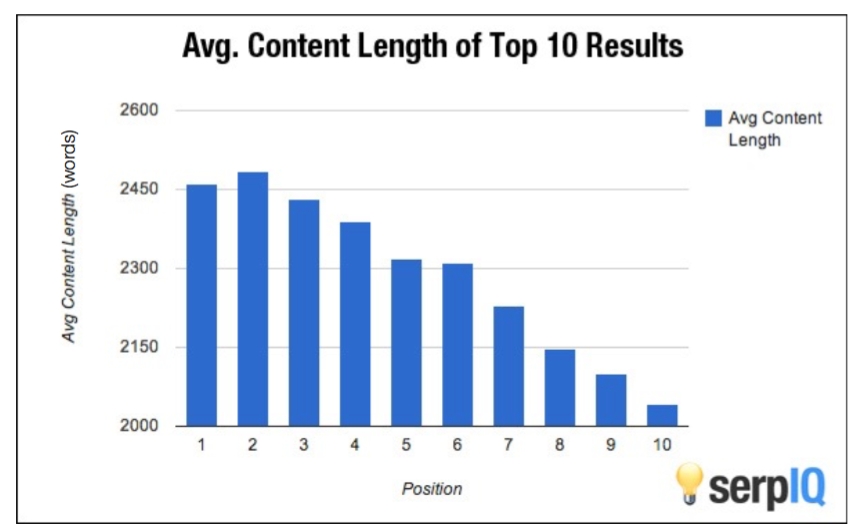
\includegraphics[width = 0.5\textwidth]{images/l23-fig-1}
	\caption{Contenuti lunghi e approfonditi sono in genere preferiti}
\end{figure}

Alcuni motori di ricerca calcolano il livello di leggibilità dei siti web, dove un alto livello di leggibilità (basso valore per il motore) indica un sito con contenuti ``\textit{facili e adatti alle masse}'' mentre un basso livello di leggibilità indica ``\textit{contenuti più complessi e elitari}''.
Non è chiaro cosa sia preferibile, ma il ranking può essere categorizzato in base a questo indice.

Anche la presenza \textbf{parole chiave} relative all'argomento del sito all'interno del contenuto è importante.

\paragraph{Title} Il tag \texttt{<title>} gioca un ruolo molto importante, sia a livello di ranking, sia perché viene mostrato tra i risultati della ricerca che vengono forniti all'utente.
\`E quindi buona norma utilizzare dei titoli correlati all'argomento della pagina, che contengano delle parole chiavi e non troppo lunghi. All'interno del titolo può anche comparire il brand del sito.

\paragraph{Meta-tag}Anche i meta-tag della sezione \texttt{head} sono molto utilizzati dai motori di ricerca e vengono utilizzati per popolare gli snippet presenti nella pagina dei risultati.
Non c'è la certezza, ma sembra che vengano apprezzati dai motori di ricerca.

\paragraph{Dimensione e immagini} La dimensione in byte della pagina gioca un ruolo fondamentale, perché viene presa sia in considerazione dai motori di ricerca che dagli utenti del sito, è quindi importante che ci sia un equilibrio tra testo e immagini.
La presenza delle immagini deve essere anche limitata perché i crawler raccolgono solo una parte della pagina, e se la parte della pagina comprende tante immagini, queste non forniscono informazioni utili.
\`E inoltre sconsigliato utilizzare delle immagini come testi per i link.

\paragraph{Struttura della pagina} I crawler preferiscono le pagine poco profonde, con una struttura semplice perché risultano più semplici da indicizzare. \`E quindi sconsigliato utilizzare le tabelle HTML ed è incentivato l'uso dei \texttt{<div>} opportunamente stilati con i CSS.
Tutto lo stile della pagina dovrebbe essere contenuto in un file CSS seprato, sia per una questione di separazione della presentazione dal contenuto, sia perché questo alleggerisce le dimensioni della pagina.
\`E inoltre importante prestare attenzione alla \textbf{site crawlability} della pagina, ovvero i contenuti dovrebbero essere facilmente accessibili dal crawler, quindi attenzione al JavaScript che potrebbe nascondere delle informazioni e niente Adobe Flash.
Sempre per facilitare il lavoro del crawler è utile specificare nel file \texttt{robot.txt} quali pagine non indicizzare, questo perché il tempo del crawler sul sito è limitato ed è meglio che eviti di sprecarlo su pagine inutili. L'utilizzo di una sitemap può agevolare ulteriormente il crawler.

\paragraph{Contesto} Il contesto geografico, temporale, sociale in cui viene effettuata una ricerca viene preso in considerazione dai motori di ricerca. Quindi possono influire positivamente sul ranking i seguenti fattori:

\begin{itemize}
	\item Indicare la città o lo stato nel tag \texttt{<title>}
	\item Il fatto che la regione del dominio o l'indirizzo fisico del server coincida con la regione in cui è stata effettuata la ricerca.
	\item Presenza della città o stato nei tag di heading.
\end{itemize}

\subsubsection{Off the page}

Anche i social network influiscono sul ranking di una pagina, infatti se una pagina viene spesso condivisa, twittata, riceve like ed è attiva sui social, il suo ranking aumenta.

L'altro fattore off the page che influisce principalmente sul ranking è l'autorevolezza del sito, determinata dai contenuti, dalla reputazione dell'autore e dallo storico del dominio. Domini più vecchi sono preferiti in quanto sono resistiti nel tempo.


\subsubsection{Riferimenti utili}

\begin{itemize}
	\item \url{http://searchengineland.com/}
	\item \url{http://moz.com/search-ranking-factors/}
\end{itemize}









% !TEX encoding = UTF-8
% !TEX TS-program = pdflatex
% !TEX root = computabilità e algoritmi.tex
% !TEX spellcheck = it-IT

\section{Funzione inversa con i corollari}

Data una funzione $ f : \mathbb{N} \rightarrow \mathbb{N} $iniettiva, totale e calcolabile. Allora

$$ 
f^{-1}(y) =\begin{cases}
x \text{ tale che } f(x) = y \\
\uparrow \text{ altrimenti}
\end{cases}
$$

è calcolabile con

$$
f^{-1}(y) = \mu x. |\: f(x) - y\:|
$$

Però se \textit{f} non è totale, non è più garantita la calcolabilità.

L'idea è quindi quella di eseguire un certo numero di passi via via crescente su ogni programma. (In teoria questa cosa è già stata fatta. Però non si poteva spiegare in modo formale).

Essendo \textit{f} calcolabile questa sarà calcolata da un certo programma \textit{e}.

$$
f^{-1}(y) = \mu (x,t). S(e, x,y, t)
$$

Peccato che non esiste un operatore che minimizza le coppie. Neanche la minimalizzazione innestata funziona, perché scorrerei la tabella prima solo sulle colonne e poi solo sulle righe.

Serve quindi un barbatrucco, in modo da riuscire a codificare una coppia con un numero intero.

$$
\mu w.  S(e, (w)_1, y, (w)_2 )
$$

Ovvero del numero \textit{w} ci interessano solo gli esponenti dei primi due divisori primi del numero.
Piccola nota: usiamo un predicato nella minimalizzazione quando sarebbe necessario utilizzare una funzione. Sarebbe quindi più corretto utilizzare il valore assoluto della funzione caratteristica del predicato, meno uno.

$$
f^{-1}(y) = \Big( \mu w.  S(e, (w)_1, y, (w)_2 ) \Big)
$$

\section{Cose non calcolabili}

Ci sono un sacco di cose che non sono calcolabili e un sacco di cose non decidibili.\\

\subsection{Totalità di un programma}

Predicato $ Tot(x) = \phi_x \text{ è totale} $ non è decidibile.

\subsubsection{Dimostrazione}

Supponiamo per assurdo che $ Tot(x) $ sia decidibile.

Definiamo

$$
f = \begin{cases}
\phi_x(x) +1 \text{ se \textit{x} è totale}\\
1 \text{ altrimenti}
\end{cases}
$$

Questa funzione è certamente totale e $ f \neq \phi_x \forall x \text{ tale che } \phi_x \text{ è totale perché se }\phi_x $ è totale $ f(x) = \phi_x(x)+1 \neq \phi_x(x) $ e quindi non è calcolabile.

Sfruttando però la totalità di \textit{Tot} è possibile scrivere la funzione $ \phi_(x) \text{ come } \Phi_U(x,x)$ e quindi \textit{f} risulterebbe definita per casi, utilizzando solamente funzioni calcolabili e quindi anch'essa sarebbe calcolabile.
Non è però possibile utilizzare la classica aritmetizzazione dell'\textit{if}, perché quando $ \phi_x $ non è totale si ha un risultato indefinito.

$$
f(x)= \bigg( \mu w. \Big( S(x,x,(w)_1, (w)_2) \wedge Tot(x) \vee (w)_1 = 0 \wedge \neg Tot(x) \Big) \bigg)_1 +1
$$

Con questa definizione il programma $ \phi_x $ vengono eseguiti sempre un po' di passi alla volta, così quando $ Tot(x) $ non è totale viene ritornato il valore corretto.

\textit{f} risulta quindi calcolabile e questo è assurdo per costruzione di \textit{f}.

\subsection{Esercizio}


\textit{Q(x)} decidibile, f1,f2 N -> N calcolabili.  f(x) = f1(x) se Q(x), f2(x) altrimenti è calcolabile?

\todo[inline]{TODO}

\subsection{Esercizio - Terminazione del programma sul suo indice}

$H(x) = \phi_x(x) \downarrow$ non è decidibile.


\section{Operazioni effettive su programmi}

Dati due programmi $ P_x, P_y $ questi calcoleranno le due funzioni $\phi_x, \phi_y$.

$$
(\phi_x + \phi_y)(z) = \phi_x(z) + \phi_y(z) = \phi_e(z) = \phi_{k(x,y)}(z)
$$

Con \textit{K} funzione totale e calcolabile.

Ovvero esiste $ K : \mathbb{N}^2 \rightarrow \mathbb{N} $ tale che $ \phi_{k(x,y)}(z) = \phi_x(z) + \phi_y(z)$.

Questo si dimostra prima utilizzando il teorema SMN:

$$
g(x,y,z) = \phi_x(z) + \phi_y(z) = \Phi_U(x,z) + \Phi_U(y,z)
$$

è calcolabile e quindi per il teorema SMN esiste $ K : \mathbb{N}^2 \rightarrow \mathbb{N} $ totale e calcolabile tale che 

$$
g(x,y,z) = \phi_{K(x,y)}(z)
$$

\subsection{Funzione inversa}

Un ragionamento simile può essere fatto con la funzione inversa.

Esiste $ K : \mathbb{N} \rightarrow \mathbb{N} $ totale e calcolabile, tale che

$$
\phi_{K(x)}(y) = (\phi_x)^{-1}(y)
$$

Definisco quindi 

$$
g(x,y) =  (\phi_x)^{-1}(y) = \Big(\mu w. S\big(x,(w)_1, y, (w)_2\big)\Big)_1
$$

\textit{g} è calcolabile e quindi per il teorema SMN si ha che esiste $ K : \mathbb{N} \rightarrow \mathbb{N} $  calcolabile e totale, tale che

$$
g(x,y,z) = \phi_{K(x,y)}(z)
$$



\subsection{Programmi con lo stesso domino}

Esiste $ K : \mathbb{N}^2 \rightarrow \mathbb{N} $ totale e calcolabile, tale che

$$
W_{K(x,y)} = W_x \cup W_y
$$

ovvero si vuole che il programma composto abbia come dominio l'unione dei due domini.

Serve quindi una funzione per l'esecuzione dei due programmi passo passo:

$$
g(x,y,z) = \mathbb{1}(\mu w. ( H(x,z,w) \vee H(y,z,w)))
$$

questa funzione è definita se \textit{z} appartiene ad almeno uno dei due domini ed è indefinita se non compare in nessuno dei due domini.

$$
g(x,y,z) = \begin{cases}
1 \text{ se } z \in W_x \cup W_y \\
\uparrow \text{ altrimenti}
\end{cases}
$$

Essendo questa funzione calcolabile, per il teorema SMN esiste una funzione $ K : \mathbb{N}^2 \rightarrow \mathbb{N} $ totale e calcolabile tale che

$$
\phi_{K(x,y)}(z) = g(x,y,z)
$$

Così facendo si ottiene proprio la funzione desiderata perché

$$
z \in W_{K(x,y)} \Leftrightarrow \phi_{K(x,y)}(z)\downarrow \Leftrightarrow z \in W_x \cup W_y
$$

\subsection{Programmi con gli stessi codomini}

Esiste $ S : \mathbb{N}^2 \rightarrow \mathbb{N} $ totale e calcolabile tale che 

$$
E_{S(x,y)} = E_x \cup E_y
$$

L'idea è quella di eseguire $ P_x $ se $ z $ è pari altrimenti se è dispari viene eseguito $ P_y $. I due programmi devono però essere eseguiti su $ z/2 $ in modo che possano essere eseguiti su tutti i numeri.

$$
g(x,y,z) =\bigg( \mu w. \Big( \big(Pari(z) \wedge S(x,z/2, (w)_1, (w)_2)\big) \vee \big( \neg Pari(z) \wedge S(y,z/2, (w)_1, (w)_2) \big) \Big) \bigg)_1
$$

Si ha quindi che la funzione 

$$
g(x,y,z) = \begin{cases}
\phi_x(z/2) \text{se \textit{z} è pari} \\
\phi_y(z/2) \text{se \textit{z} è dispari}
\end{cases}
$$

è calcolabile per come è stata precedentemente definita. (Sarebbe da ricopiare la definizione, utilizzando \textit{qt} al posto della divisione classica).

Essendo calcolabile segue che per il teorema SMN esiste $ S : \mathbb{N}^2 \rightarrow \mathbb{N} $ calcolabile e totale, tale che

$$
\phi_{S(x,y)}(z) = g(x,y,z)
$$

ed è la funzione cercata perché:

$$
v \in E_{S(x,y)} \Rightarrow \exists z | \phi_{S(x,y)}(z) = v \Rightarrow \begin{cases}
g(x,y,z) = v = \phi_x(z/2) \text{ se \textit{z} è pari} \Rightarrow v \in E_x \\
g(x,y,z) = v = \phi_y(z/2) \text{ se \textit{z} è dispari} \Rightarrow v \in E_y 
\end{cases} \Rightarrow v \in E_x \cup E_y
$$

e vale anche l'altra inclusione, perché, sia $ v \in E_x $, esiste $ z $ tale che $ \phi_x(z) = v  \Rightarrow \phi_{S(x,y)}(2z) = g(x,y,2z) = \phi_x(z)$ e siccome per un qualche argomento \textit{z} si ha che $ v \in E_{S(x,y)} $.


\section{Esercizi}

\begin{enumerate}
	\item Esiste $ K : \mathbb{N} \rightarrow \mathbb{N} $ calcolabile e totale, tale che $ E_{K(x)} = W_x $?
	\item Data $ f : \mathbb{N} \rightarrow \mathbb{N} $ calcolabile, esiste $ K : \mathbb{N} \rightarrow \mathbb{N} $ calcolabile e totale, tale che $ \forall x \: W_{K(x)} = f^{-1}(W_x) $
\end{enumerate}








% !TEX encoding = UTF-8
% !TEX TS-program = pdflatex
% !TEX root = computabilità e algoritmi.tex
% !TEX spellcheck = it-IT

\chapter{Insiemi Ricorsivi e Ricorsivamente Enumerabili}

Ogni proprietà interessante del comportamento dei programmi non è calcolabile (correttezza, assenza di bug, terminazione).


Dal punto di vista della computabilità tutti i problemi decidibili vengono considerati facili, anche se richiedono un carico computazionale estremamente elevato.

Ci sono poi i problemi semi-decidibili, per i quali si riesce a rispondere solo in caso positivo e i problemi indecidibili per i quali non è sempre possibile fornire una risposta.

\section{Insiemi}

Dato un sottoinsieme $ X \subseteq \mathbb{N} $, $ x \in X $? Quando questa proprietà è decidibile si dice che l'insieme è \textbf{ricorsivo}, mentre se è semi-decidibile, l'insieme è \textbf{ricorsivamente enumerabile}.

La definizione utilizza i numeri, ma per noi questi possono essere considerati come dei programmi:

$$
X = \{ x | P_x \ldots \}
$$

\subsection{Insiemi ricorsivi}

$A \subseteq \mathbb{N}$ si dice ricorsivo se la sua funzione caratteristica

$$
\mathcal{X}_A : \mathbb{N} \rightarrow \mathbb{N}
$$ 

che vale 1 se $ x \in A $ e 0 altrimenti è calcolabile, ovvero se il predicato $ x \in A $ è decidibile.

$\mathbb{N}$ è ricorsivo, perché la sua funzione caratteristica è la costante 1.

$P_r = \{x | x \text{ è primo}\}$ è anche esso ricorsivo.

Come risultato più generale si ha che tutti gli insiemi $ A \subseteq \mathbb{N} $ e finiti sono ricorsivi, perché la loro funzione caratteristica può essere sempre definita come una serie di \textit{if}.

L'insieme $ K = \{ x | \phi_x(x)\downarrow \} $ non è ricorsivo, perché se per assurdo lo fosse, sarebbe possibile definire una funzione calcolabile diversa da tutte quelle calcolabili:

$$
f(x) = \begin{cases}
\phi_x(x)+1 &x \in K \\
1 & x \notin K
\end{cases}
$$

la funzione così definita è totale e calcolabile, perché può essere definita come 

\begin{align*}
f(x) &= (\mu w. (x in K \wedge (w)_1 = \phi_x(x) \wedge (w)_2 = \text{ numero di passi per termianre}) \vee (x \notin K \wedge (w)_1 = 0))_1 +1 \\
&= (\mu w. (x \in K \wedge S(x,x,(w)_1, (w)_2)) \vee (x \notin K \wedge (w)_1 = 0))_1 +1
\end{align*}

e per combinazione di funzione calcolabili e minimalizzazione è calcolabile. $f$ risulta quindi calcolabile e questo è un problema perché

$$
\forall x \phi_x(x) \begin{cases}
x \in K & f(x) = \phi_x(x) +1 \neq \phi_x(x) \\
x \notin K & f(x) = 1 \neq \phi_x(x)\uparrow
\end{cases}
$$

quindi $ K $ non può essere ricorsivo.

Anche $T = \{x |  \phi_x \text{ è totale}\}$ non è ricorsivo.

\subsubsection{Chiusura degli insiemi ricorsivi}

Se $ A $ e $ B $ sono due insiemi ricorsivi, anche

\begin{itemize}
	\item $ \bar{A} = \mathbb{N} \ A$
	\item $ A \cup B $
	\item $ A \cap B$
\end{itemize} 

sono ricorsivi.

\section{Riduzione}

Si hanno due problemi, $ \mathcal{A} $ e $ \mathcal{B} $ e si vuole poter dire se $ \mathcal{A} $ è più facile o più difficile di $ \mathcal{B} $.

Questo prende il nome di \textbf{m-riducibilità}\footnote{Ometteremo il prefisso m-.} e con questo si intende che dati $ A,B \subseteq \mathbb{N} $, il problema $ x \in A $ si riduce al problema $ x \in B $ (notazione $ A \leq_m B $) se esiste $ f : \mathbb{N} \rightarrow \mathbb{N} $ calcolabile e totale, tale che $ \forall x \: x \in A \Leftrightarrow f(x) \in B$.

Ovvero esiste un modo che permette di trasformare un'istanza del problema $ \mathcal{A} $ in un'istanza del problema $ \mathcal{B} $ tale che se l'istanza $ x $ soddisfa $ \mathcal{B} $, questa soddisfa anche $ \mathcal{A} $.

In questo caso il problema $ \mathcal{A} $ è più facile da risolvere perché sapendo risolvere il problema $ \mathcal{B} $ si riesce a risolvere anche $ \mathcal{A} $.

Più formalmente, se $ A, B \subseteq \mathbb{N} \: A \leq_m B $ allora

\begin{enumerate}
	\item se $ B $ è ricorsivo anche $ A $ è ricorsivo
	\item se $A $ non è ricorsivo, anche $ B $ non è ricorsivo
\end{enumerate}

Il punto 1 si dimostra a partire dalla funzione caratteristica di \textit{B}: se \textit{B} è ricorsivo,

$$
\mathcal{X}_B(x) = \begin{cases}
1 & x \in B \\
0 & x \notin B
\end{cases}
$$

la funzione caratteristica di $ A $ può essere definita come

$$
\mathcal{X}_A(x) = \begin{cases}
1 & x \in A \\
0 & x \notin A
\end{cases} = \mathcal{X}_B(f(x))
$$

Il punto 2 si dimostra in modo simile.

L'insieme $ T = \{x | \phi_x(x) \text{totali}\} $ non è ricorsivo e può essere dimostrato utilizzando la riduzione $ K \leq_m T $\footnote{la \textit{m} si può omettere}.

\`E quindi necessario trovare una funzione $ f : \mathbb{N} \rightarrow \mathbb{N} $ calcolabile e totale, tale che $ x \in K $ se e solo se $ f(x) \in T $.
Vogliamo quindi una funzione che fornisca sempre un output se $ x \in K (P_x(x)\downarrow)$ e che non fornisca mai un output se $ x \notin K $.

Possiamo quindi definire una funzione $ g(x,y) $ con $ x $ il programma da trasformare e $ y $ l'input di tale programma (che non verrà mai usato).

$$
g(x,y) = \begin{cases}
\phi_x(x) & x \in K \\
\uparrow & \text{ altrimenti}
\end{cases} = \phi_x(x) = \Phi_U(x,x)
$$

essendo $ g $ calcolabile, per il teorema SMN esiste una funzione $f : \mathbb{N} \rightarrow \mathbb{N}$ calcolabile e totale tale che

$$
g(x,y) = \phi_{f(x)}(y)
$$

$ f $ è quindi una funzione di riduzione di $ K $ a $ T $ perché se $ x \in K $, $ f(x) \in T $ si ha  $\phi_{f(x)}(y) = g(x,y) = \phi_x(x)\downarrow \forall y$ totale ($f \in T$), viceversa se $ x \notin K $, $f(x) \notin T$ perché $\phi_{f(x)}(y) = g(x,y) = \phi_x(x) \uparrow \forall y$ e non è totale, quindi $f \notin T$.

Quindi $ K \leq_m T $ tramite $ f $, pertanto essendo $ K $ non ricorsivo neppure $ T $ lo sarà.

\subsection{Problema dell'input}

$$
A_n = \{ x | \phi_x(n)\downarrow \}
$$

Per un \textit{n} fissato, questo insieme non è ricorsivo e lo si dimostra per riduzione con $ K \leq_m A_n $.

Serve quindi una funzione \textit{S} calcolabile e totale, tale che se $ x \in K $, $ f(x) \in A_n $, ovvero si vuole trasformare un programma $ P_x $ in un altro programma che prende in input un valore $ y $ e che se $x \in K$ allora $P_{f(x)}(n)\downarrow$ e che se $ x \notin K $, $P_{f(x)}(n)\uparrow$.

In modo simile a prima è possibile definire

$$
g(x,y) = \phi_x(x) = \Phi_U(x,x)
$$

per il teorema SMN esiste quindi $ S : \mathbb{N} \rightarrow \mathbb{N} $ calcolabile e totale, tale che 

$$
g(x,y) = \phi_{S(x)}(y)
$$

$ S $ è la funzione di riduzione di $ K $ a $ A_n $ perché se $ x \in K $, $ \phi_{S(x)}(y) = g(x,y) = \phi_x(x)\downarrow $ e in particolare $\phi_{S(x)}(n) = \phi_x(n) $ che è definita e quindi $S(x) \in A_n$.

Se invece $ x \notin K $, $\phi_{S(x)}(y) = \phi_x(x)\uparrow \forall y$ e quindi, per definizione di $A_n$ si ha che $S(x) \notin A_n$

\subsection{Problema dell'output}

$$
B_n = \{ x | n \in E_x \}
$$

Per un \textit{n} fissato, questo insieme non è ricorsivo e lo si dimostra per riduzione con $ K \leq_m B_n $.

Serve quindi una funzione \textit{f} tale che $ x \in K \Leftrightarrow f(x) \in B_n$.

La dimostrazione è uguale a quella precedente con la differenza che il programma $ P_{f(x)}(x) $ deve sempre ritornare \textit{n}:

$$
g(x,y) = \begin{cases}
n & x \in K \\
\uparrow & \text{ altrimenti} 
\end{cases} = n \cdot 1(\phi_x(x))
$$ 

Essendo calcolabile, per il teorema SMN esiste $ f : \mathbb{N} \rightarrow \mathbb{N} $ calcolabile e totale, tale che 

$$
g(x,y) = \phi_{f(x)}(y)
$$

$f$ è la funzione di riduzione di $ K \leq_m B_n $ perché se $ x \in K  $, $\phi_{f(x)}(y) = g(x,y) = n $ che certamente ha $ n $ nel suo codominio ($ n \in E_{f(x)} = \{n\}$) e quindi $f(x) \in B_n$.
Se invece $ x \notin K $, $\phi_{f(x)}(y) \uparrow = g(x.y) \forall y $, ovvero $E_{f(x)} = \emptyset $ e quindi $f(x) \notin B_n$.



% !TEX encoding = UTF-8
% !TEX TS-program = pdflatex
% !TEX root = computabilità e algoritmi.tex
% !TEX spellcheck = it-IT

\section{Teorema di Rice}

Ogni proprietà del comportamento di un programma non è decidibile (es: il programma termina sempre, termina in un certo input, ecc.).
Queste proprietà sono quelle che riguardano che cosa calcola il programma, non come è definito.

Un \textbf{insieme saturato} (versione formale delle proprietà dei programmi) $ A \subseteq \mathbb{N} $ tale che se $ x \in A $ e $ y \in \mathbb{N} $ e tale che $ \phi_x = \phi_y $, allora anche $ y \in A $.

$ A $ è saturato se e solo se esiste $ \mathcal{A} \subseteq \mathcal{C} $ tale che $ A = \{ x | \phi_x \in A \} $, ovvero il fatto che un programma appartenga ad un insieme saturo non dipende dalla struttura del programma ma dalla funzione che esso calcola.

Ad esempio $ T = \{ x | \phi_x \text{ è totale} \} $ è un insieme saturo, perché la proprietà che un programma termina è come dire che la funzione calcolata dal programma termina sempre.

Anche $ \{ x | \phi_x = \lambda y . \sqrt{y} \} $ è saturo, perché contiene tutte le funzioni che calcolano la radice quadrata.

$ K = \{ x | x \in W_x \} $ non è saturo perché intuitivamente non si riesce definire in modo preciso un insieme di funzioni. L'idea è quella di mostrare che esiste una funzione calcolabile $ e \in \mathbb{N} $ tale che

$$
\phi_e(x) = \begin{cases}
e &\:x=e \\
\uparrow &\:\text{altrimenti}
\end{cases}
$$ 

per come è definita questa funzione $ e \in W_e \Rightarrow e \in K$ ed esiste $ e' \in \mathbb{N} $ tale che $ \phi_e = \phi_{e'} $ e $ e \neq e' $.

Si ha che $\phi_{e'}(e') = \phi_e(e') = \uparrow$ e quindi $ e' \notin K $, ovvero l'insieme $ K $ non contiene tutti gli indici che calcolano la stessa funzione.

Tutto questo si basa sul fatto che $ e $ esiste e arriveremo più avanti a dimostrarlo.

\subsection{Enunciato del teorema di Rice}

Sia $ A $ una qualunque proprietà del comportamento dei programmi, ovvero $ A \subseteq \mathbb{N} $ e saturo.

Se la proprietà non è banale, l'insieme non è ricorsivo.

Con proprietà non banale si intente $ A \neq \mathbb{N}$ (sempre vera) e $ A \neq \emptyset $ (sempre falsa).

\subsubsection{Dimostrazione}

L'obiettivo è quello di dimostrare che $ K \leq_m A $.

Per ipotesi sappiamo che $ A $ non è vuoto e non è tutto $ \mathbb{N} $, quindi è definito anche l'insieme $ \bar{A} $.
Vogliamo trovare una funzione $ f : \mathbb{N} \rightarrow \mathbb{N} $ calcolabile e totale tale che $ x \in K \Leftrightarrow f(x) \in A$.

Consideriamo un qualunque indice $ e_0 \in \mathbb{N} \: \phi_{e_0} = \emptyset$ ovvero che non termina mai.

Ci sono due possibili casi:

\begin{enumerate}
	\item $e_0 \in \bar{A}$: sia $ e_1 \in A $ un programma qualsiasi (che sappiamo esistere perché $ \bar{A} \neq \emptyset$). Possiamo definire
	$$
	g(x,y) = \begin{cases}
	\phi_{e_1}(y) & x \in K\\
	\phi_{e_0}(y) & x \notin K
	\end{cases} = \begin{cases}
	\phi_{e_1}(y) & x \in K \\
	\uparrow & x \notin K
	\end{cases} = \phi_{e_1}(y) \cdot 1(\phi_x(x))
	$$
	che è calcolabile perché può essere scritta utilizzando la funzione calcolabile. Perciò è possibile utilizzare il teorema SMN per avere la garanzia dell'esistenza di una funzione $ f : \mathbb{N} \rightarrow \mathbb{N} $ calcolabile e totale, tale che $ g(x,y) = \phi_{f(x)}(y)  \forall x,y$, che può essere utilizzata come funzione di riduzione. Questo perché se $ x \in K \Rightarrow \phi_{f(x)}(y) = \phi_{e_1}(y) \forall y$ e dato che $ A $ è saturato e che $ e_1 \in A $, allora anche $ f(x) \in A$ perché essendo saturo $ A $ contiene tutti gli indici che calcolano quella funzione. Se invece $ x \notin K \Rightarrow \phi_{f(x)}(y) = \phi_{e_0} \forall y$ e allo stesso modo dato $ e_0 \notin A $ anche $ f(x) \notin A $ perché se questo non fosse vero anche $ e_0 $ dovrebbe appartenere ad $ A $.  Concludendo, dato che $ K $ non è ricorsivo e che $ K \leq_m A $, anche $ A $ non è ricorsivo.
	\item $e_0 \in A$: sia $ B = \bar{A} $, $ B \neq \emptyset \neq \mathbb{N} $ e saturo perché è l'insieme complementare di un insieme saturo ed $ e_0 \notin B $. Per quanto dimostrato al punto 1, si ha che $ B $ non è ricorsivo e quindi anche $ \bar{A} $ non è ricorsivo, allora anche $ A $ non è ricorsivo perché è l'insieme complementare di un insieme ricorsivo.
\end{enumerate}


$ A_n = \{ x | n \in W_x \}  = \{ x | \phi_x(n) \downarrow  \}$ è saturo perché può essere visto come

\begin{align*}
A_n &= \{ x | \phi_x \in \mathcal{A}_n \}  \\
\mathcal{A}_n &= \{ f \in \mathcal{C} | n \in dom(f) \} 
\end{align*} 

Si ha poi che 
\begin{enumerate}
	\item $ A_n \neq \emptyset $: $ e_1 $ tale che $ \phi_{e_1} = id $, $ e_1 \in A_n $ 
	\item $A_n \neq \mathbb{N}$: $e_0$ tale che $ \phi_{e_0} = \emptyset $, $ e_0 \notin A $
\end{enumerate}


Quindi per il teorema di Rice $ A_n $ non è ricorsivo.

$ B_n = \{  x | n \in E_x\} $ è saturo, perché $ B_n  = \{ x | x \in \mathcal{B}_n\}$ con $ \mathcal{B}_n = \{ f \in \mathcal{C} | n \in cod(f) \} $ e:
\begin{itemize}
	\item $ B_n \neq \emptyset $ se $ e_1 $ tale che $ \phi_{e_1} = id \: n \in E_{e_1} = \mathbb{N} \Rightarrow e_1 \in B_n$ 
	\item $ B_n \neq \mathbb{N} $ se $ e_0 $ tale che $\phi_{e_0} = \emptyset \: n \notin E_{e_0} \Rightarrow e_0 \notin B_n$ 	
\end{itemize}

Quindi per il teorema di Rice anche $ B_n $ non è ricorsivo.


Sia $ f : \mathbb{N} \rightarrow \mathbb{N} $ una funzione $ B_f = \{ x | \phi_x = f \} $ è saturo per definizione e per il teorema di Rice non è ricorsivo a meno che $ f \notin \mathcal{C} $ perché in quel caso si ha $ B_f = \emptyset $. Infatti, se $ f \in \mathcal{C} $, $ B_f \neq \emptyset $ perché banalmente esiste un programma che non la calcola. $ B_f \neq \mathbb{N} $ perché sia $ e_2 $ tale che $ \phi_{e_2} \neq f$ ed esiste perché le funzioni calcolabili sono infinite si ha che $ e_2 \notin B_f $.
Quindi per Rice $ B_f $ non è ricorsivo.


$ C = \{ x | x \in W_x \cap E_x \} $ non sappiamo se questo insieme è saturato, ma intuitivamente se proviamo a definire $ C = \{x | \phi_x \in \mathcal{A} \} $ abbiamo dei problemi a definire $ \mathcal{A} $.

Mostrare che $ K \leq_m C $.
\todo[inline]{TODO}

$ D = \{ x | E_x infinito \}$ dire se è ricorsivo o meno
\todo[inline]{TODO}

\section{Insiemi ricorsivamente enumerabili (RE)}

$A \subseteq \mathbb{N}$ è \textbf{RE} se la sua funzione semi-caratteristica è calcolabile:

$$
SC_A(x) = \begin{cases}
1 & x \in A \\
\uparrow & x \notin A
\end{cases}
$$

Il fatto che un insieme $ A $ è RE equivale a dire che il predicato ``$ x \in A $'' è semi-decidibile.

\subsection{ Ricorsivo $\subseteq $ RE} 

Se $ A \subseteq \mathbb{N} $ è ricorsivo $\Leftrightarrow A, \bar{A}$ sono ricorsivamente enumerabili.

\subsubsection{$A \text{ ricorsivo } \Rightarrow A \text{ RE}$}

Sia $ A $ ricorsivo, allora la sua funzione caratteristica è 

$$
\mathcal{X}_A(x) = \begin{cases}
1 &x \in A \\
0 & x \notin A
\end{cases}
$$

allora 

$$
SC_A = 1\Big( \mu w \overline{\text{sg}}\big( \mathcal{X}_A(x) \big) \Big)
$$

è definita per minimalizzazione di una combinazione di funzione calcolabili e pertanto è anch'essa calcolabile.

Per dimostrare che anche $ \bar{A} $ è ricorsivamente enumerabile basta osservare che se $ A $ è ricorsivo anche il suo complementare $\bar{A} $ è ricorsivo e quindi per quanto dimostrato finora è anche ricorsivamente enumerabile.

\subsubsection{$A, \bar{A} \text{ RE } \Rightarrow A \text{ ricorsivo}$}

Dato che $ A \text{ e } \bar{A} $ sono RE e quindi $ SC_A $ e $ SC_{\bar{A}} $ sono calcolabili.

Si possono quindi trovare $ e_1, e_0 $ tali che $ \phi_{e_1} = SC_A1 $ e $ \phi_{e_0} = SC_{\bar{A}} $.

Intuitivamente è possibile definire un programma che esegue in parallelo entrambi i programmi sull'input $ x $ e attende che uno dei due programmi termini. Se termina prima $ e_1 $ ritorna 1, altrimenti se termina $ e_0 $ ritorna 0.

Per fare questo con una macchina URM serve un $ e_0 $ leggermente diverso, ovvero tale che $ \phi_{e_0} = \overline{\text{sg}} \cdot SC_{\bar{A}} $.
Così facendo la funzione ritorna 0 quando $ x \in \bar{A} $.

La funzione calcolata dal programma che esegue i due programmi in parallelo può essere definita come:

$$
\mathcal{X}_A = \bigg( \mu w. S\Big(e_1, x, (w)_1, (w)_2\Big) \vee S\Big(e_0, x, (w)_1, (w)_2\Big) \bigg)
$$

e risulta essere calcolabile.














% !TEX encoding = UTF-8
% !TEX TS-program = pdflatex
% !TEX root = computabilità e algoritmi.tex
% !TEX spellcheck = it-IT

\subsection{L'insieme $K$}

$$ 
K= \{x | x \in W_x \} = \{ x | \phi_x(x) \downarrow \}
$$

è ricorsivamente enumerabile anche se non è ricorsivo perché 

$$
SC_K(x) = \begin{cases}
1 x \in K \\
\uparrow \text{ altrimenti}
\end{cases} = \begin{cases}
1 \phi_x(x)\downarrow \\
\uparrow \: \text{altrimenti}
\end{cases} = 1(\phi_x(x))
$$

che può essere calcolata utilizzando la funzione universale.

Banalmente $\overline{K}$ non è ricorsivamente enumerabile perché se lo fosse, $K$ sarebbe ricorsivo e sappiamo che non lo è.

\subsection{Teorema di struttura dei predicati semidecidibili}

Sia $P(\vec{x})$ un predicato $k$-ario, $P(\vec{x})$ è semidecidibile se e sole se esiste $Q(t,\vec{x})$ decidibili tale che $P(\vec{x}) \equiv \exists t Q(t,\vec{x})$.

Ovvero il predicato $P$ è una generalizzazione di un predicato decidibile che viene calcolato su più punti.

In generale, quantificare esistenzialmente trasforma un predicato decidibile in uno semidecidibile.

\subsubsection{Dimostrazione}

Supponiamo che $P(\vec{x}) \equiv Q(t,\vec{x})$ con $Q$ decidibile. La funzione caratteristica di $P$ non farà altro che cercare la un $t$ utilizzando una minimalizzazione illimitata.

$$
SC_P(\vec{x}) = \begin{cases}
1 \text{ se } P(\vec{x}) \\
\uparrow \text{ altrimenti} 
\end{cases} = 1 \big(\mu t. \text{``}Q(t,\vec{x})\text{''} \big) = 1\big( \mu t . |\mathcal{X}_Q(t,\vec{x})  - 1| \big)
$$

$SC_P$ è calcolabile perché $\mathcal{X}_Q$ è calcolabile per ipotesi e quindi $P\vec{x}$ è semidecidibile.

Viceversa, sia $P(\vec{x})$ semidecidibile, allora anche $SC_P(\vec{x})$ è calcolabile, ovvero $SC_P = \phi_e$ per qualche $e \in \mathbb{N}$.

Il predicato $P(\vec{x})$ vale se e solo se $SC_P(\vec{x}) = \phi_e(\vec{x}) = 1 \Leftrightarrow \phi_e(\vec{x})\downarrow \Leftrightarrow \exists t . H(e, \vec{x}, t)$, dove $H$ è la funzione che ritorna 1 se la macchina $e$ termina in $t$ passi sull'input $\vec{x}$ che sappiamo essere decidibile.

Indicando con $Q(t,\vec{x}) \equiv H^{(k)}(e, \vec{x},t)$ decidibile e $P(\vec{x}) \equiv \exists t Q(t,\vec{x})$.

\subsection{Chiusura per quantificazione esistenziale (teorema di proiezione)}

La classe degli insiemi ricorsivamente enumerabili è chiusa rispetto la quantificazione esistenziale.

Dato $P(x,\vec{y}) \subseteq \mathbb{N}^{k+1}$ semidecidibile, allora anche $P'(\vec{y}) \equiv \exists x. P(x,\vec{y})$ è semidecidibile.

\subsubsection{Dimostrazione}

Per ipotesi $P(x,\vec{y})$ è semidecidibile e quindi per il teorema di struttura può essere espresso come

$$
P(x,\vec{y}) = \exists t . Q(t,x, \vec{y})
$$

 con $Q$ decidibile e utilizzando ciò è possibile definire:
 
 $$
 P'(x,\vec{y}) \equiv \exists x.\exists t . Q(t,x, \vec{y}) \equiv \exists w . \underbrace{Q((w)_1, (w)_2, \vec{y})}_{Q'}
 $$
 
 con $Q'(w,\vec{y}) \equiv Q((w)_1, (w)_2, \vec{y})$, che ha come funzione caratteristica $\mathcal{X}_{Q'} = \mathcal{X}_Q((w)_1, (w)_2, \vec{y})$ calcolabile.
 
 Si ha quindi che $Q'$ è decidibile e quindi per il teorema di struttura $P'(\vec{y})$ è semidecidibile.
 
 \subsection{Chiusura per and e or}
 
 Siano $P_1(\vec{x})$ e $P_2(\vec{x})$ semidecidibili, allora:
 
 \begin{enumerate}
 	\item $P_1(\vec{x}) \vee P_2(\vec{x})$
 	\item $P_1(\vec{x}) \wedge P_2(\vec{x})$
 \end{enumerate}
 
 sono semidecidibile.
 
 \subsubsection{Dimostrazione}
 
 Per il teorema di struttura possiamo vedere i due predicati come la quantificazione esistenziale di due predicati $Q_1$ e $Q_2$ decidibili.
 
 Si ha quindi che i due predicati possono essere visti come
 
 \begin{enumerate}
	 \item $P_1(\vec{x}) \vee P_2(\vec{x}) = \exists t Q_1(t,\vec{x}) \vee \exists t Q_2(t,\vec{x}) = \exists t ( Q_1(t,\vec{x}) \vee Q_2(t,\vec{x}))$
	 \item  $P_1(\vec{x}) \wedge P_2(\vec{x}) = \exists t Q_1(t,\vec{x}) \wedge \exists t Q_2(t,\vec{x}) = \exists w ( Q_1((w)_1,\vec{x}) \wedge Q_2((w)_2,\vec{x}))$
 \end{enumerate}
 
 Siccome i predicati $Q_1$ e $Q_2$ sono decidibili, anche le loro congiunzioni/disgiunzioni sono decidibili e quindi, sempre per il teorema di struttura, la congiunzione e la disgiunzione di predicati semidecidibili è semidecidibile.
 
 \subsection{La quantificazione universale}
 
 La quantificazione universale è rognosa da trattare perché anche un predicato decidibile, se viene quantificato universalmente può diventare non semidecidibile.
 
 Intuitivamente questo è vero perché risulta indefinito andare a testare un predicato su infiniti valori.
 
 Ad esempio $Q(t,x) \equiv \neg H(x,x,t)$ è decidibile, ma $Q'(x) \equiv \forall t . Q(t,x) \equiv \phi_x(x) \uparrow \equiv x \in \overline{K}$ che non è neanche semidecidibile.
 
 Si ha anche che $x \in K$ è semidecidibile ma $\neg (x \in K) \equiv x \in \overline{K}$ non semidecidibile. 
 
 \subsection{Riducibilità per gli insiemi RE}
 
 Dati due insiemi $A,B \subseteq \mathbb{N}$ e $A \leq_m B$
 
 \begin{enumerate}
 	\item se $B$ è RE $\Rightarrow A$ è RE
 	\item  se $A$ non è RE $\Rightarrow B$ non è RE 
 \end{enumerate}
 
 Questo può essere utilizzato per dimostrare che $A$ è ricorsivamente enumerabile, con la riduzione $A \leq_m K$ oppure che $A$ non è ricorsivamente enumerabile $\overline{K} \leq_m A$.
 
 \subsubsection{Dimostrazione}
 
Per il primo punto: sia $f : \mathbb{N} \rightarrow \mathbb{N}$ calcolabile e totale e $x \in A \Leftrightarrow f(x) \in B$ per riduzione, allora 

$$
SC_A(x) = SC_B(f(x))
$$

è calcolabile per composizione di funzioni calcolabili e quindi $A$ è RE.

L'altro caso è analogo.

\subsection{Perché RE? (Teorema di etimologia)}

Da dove deriva il nome ricorsivamente enumerabili?

L'enumerabile deriva dal fatto che esiste una funzione $f : \mathbb{N} \rightarrow A$ suriettiva che equivale a dire che $f : \mathbb{N} \rightarrow \mathbb{N}$, totale e tale che $cod(f) = A$.

Il ricorsivo invece richiama il fatto che l'enumerazione può essere fatta con una funzione calcolabile.

Si ha quindi che l'insieme degli insiemi ricorsivamente enumerabili è effettivamente ricorsivamente enumerabile.

\subsubsection{Dimostrazione}

Sia $A \subseteq \mathbb{N}$, $A$ è RE se e solo se $A = \emptyset $ oppure esiste $f : \mathbb{N} \rightarrow \mathbb{N}$ calcolabile, totale e tale che $A = cod(f)$.

\paragraph{$\Rightarrow$}

Sia $A$ RE.

Se $A = \emptyset$ il teorema è trivialmente vero.

Se $A \neq \emptyset$, sia $a_0 \in A$ fissato e sia $e$ un programma tale che $\phi_e = SC_A$.

Il programma \textit{e} può essere modificato in modo che possa eseguire al massimo $t$ passi e che ritorni $x$ se $x \in A$ e riesce a deciderlo in massimo $t$ passi, altrimenti ritorna $a_0$. Si ha quindi che $\phi_{e'}$ ha come codominio $A$ ed è totale.

Più formalmente

$$
f(w) = \begin{cases}
(w)_1 \text{ se } H(e, (w)_1, (w)_2) \\
a_0 \text{ altrimenti}
\end{cases} = (w)_1 \mathcal{X}_H(e, (w)_1, (w)_2) + a_0 \: | \:1 - \mathcal{X}_H(e, (w)_1, (w)_2)\:|
$$ 

$f$ è totale perché è sempre definita ed è calcolabile perché è la composizione di funzioni calcolabili.

Inoltre, $A = cod(f)$ perché se $x \in A \Rightarrow \phi_e(x) = SC_A(x) = 1$ e quindi esiste un numero finito di passi $t$ entro i quali l'esecuzione di $e$ termina. Sia $w \in \mathbb{N}$ tale che $(w)_1 = x$ e $(w)_2 = t$, si ha che $f(w) = x$ e che $x \in cod(f)$.
$w$ esiste e ce ne sono possibilmente infiniti, perché basta un numero naturale tale che $w = 2^x \cdot 3^t \cdot \ldots $

Viceversa se $z \in cod(f)$, $z = f(w)$ per un qualche $w \in \mathbb{N}$. Ci sono quindi due possibilità:

\begin{enumerate}
	\item $f(w) = a_0 \in A$
	\item $f(w) = (w)_1 \rightsquigarrow H(e, (w)_1, (w)_2) \Rightarrow \phi_e((w)_1) \downarrow \Rightarrow SC_A((w)_1) = 1$ e quindi $z = (w)_1 \in A$.
\end{enumerate}

\paragraph{$\Leftarrow$}

Se $A = \emptyset$, $A$ è ricorsivo e quindi è anche RE.

Se $A = cod(f)$ con $f$ calcolabile e totale.

$$
SC_A(x) = 1 \big( \mu w. |f(w) - x| \big)
$$

definita per composizione di funzioni calcolabili e quindi è calcolabile il che implica che $A$ è RE.

\section{Teorema di Rice-Shapiro}

Le proprietà del comportamento (funzione calcolata) dei programmi possono essere semidecidibili se sono sono finitarie ovvero dipendono da un numero finito di argomenti.

Ad esempio ``\textit{la funzione termina su 5}'' oppure ``\textit{la funzione termina in un punto}'' sono semidecidibili.

\textbf{Funzione finita}: $\theta : \mathbb{N}  \rightarrow \mathbb{N}$ tale che $dom(\theta)$ è finito, ovvero è una funzione definita solamente su un insieme finito di elementi.

\textbf{Pezzo di una funzione}: date due funzioni $f,g : \mathbb{N} \rightarrow \mathbb{N}$, \textit{f} è un pezzo di $g$, $f \subseteq g$ se $\forall x . f(x) \downarrow \Rightarrow g(x) \downarrow \text{ e } f(x) = g(x) $.

Più formalmente:

Sia $\mathcal{A} \subseteq \mathcal{C}$ e sia $A = \{ x | \phi_x \in \mathcal{A} \}$.

Se $ A $ è ricorsivamente enumerabile, allora $\forall f \in \mathcal{C} . \Big( f \in \mathcal{A} \Leftrightarrow \exists \theta \subseteq f \in \mathcal{A} \Big)$.


% !TEX encoding = UTF-8
% !TEX TS-program = pdflatex
% !TEX root = computabilità e algoritmi.tex
% !TEX spellcheck = it-IT

%\section{Teorema di Rice Shapiro}

\subsection{Dimostrazione}

La dimostrazione è qualcosa del tipo

\begin{enumerate}
	\item $\exists f \: f \notin \mathcal{A} \text{ e } \exists \theta \subseteq f \: \theta \in \mathcal{A} \Rightarrow A$ non è RE
	\item $\exists f \: f \in \mathcal{A} \text{ e } \forall \theta \subseteq f \: \theta \notin \mathcal{A} \Rightarrow A$ non è RE
\end{enumerate}
	
\subsubsection{Dimostrazione caso 1}

 $$
 \exists f \: f \notin \mathcal{A} \text{ e } \exists \theta \subseteq f \: \theta \in \mathcal{A} \Rightarrow A \text{ non è RE }
 $$
 
 Sia $f \notin \mathcal{A}$ e sia $\theta \subseteq f \: \theta \in \mathcal{A}$.
 
 Per provare che $A$ non è RE possiamo provare a fare la riduzione $\overline{K} \leq_m A$. 
 
 Definiamo quindi 
 
\begin{align*}
 g(x,y) &= \begin{cases}
 \theta(y) x \in \overline{K} \\
 f(y) x \in K
 \end{cases} \\
  &= \begin{cases}
 \uparrow x \in \overline{K} \text{ e } y \notin dom(\theta)\\
 f(y) x \in \overline{k} \text{ e } y \in dom(\theta) \\
 f(y) x \in K
 \end{cases} \\
 &=\begin{cases}
  f(y) x \in K \text{ oppure } y \in dom(\theta) \\
  \uparrow \text{ altrimenti}
 \end{cases}
 \end{align*}
 
$x \in K$ è semidecidibile, quindi il predicato $Q(x,y) \equiv \text{``}x \in K\text{''}\vee \text{``}y \in dom(\theta)\text{''}$ è semidecidibile.
 
Si può quindi definire $g$ come:

$$
g(x,y) = f(y) \cdot SC_Q(x,y)
$$
 
 e dato che sia la funzione caratteristica, sia $f$ sono calcolabili, anche $g$ è calcolabile.
 
 Essendo calcolabile, per il teorema SMN $ g(x,y) = \phi_{S(x)}(y)$ per $S : \mathbb{N} \rightarrow \mathbb{N}$. $S$ è quindi una funzione di riduzione per $\overline{K} \leq_m A$:
 
 \begin{itemize}
 	\item $x \in \overline{K}$: $\phi_{S(x)}(y) = g(x,y) = \begin{cases}
 	 f(y) x \in K \text{ oppure } y \in dom(\theta) \\
 	 \uparrow \text{ altrimenti}
 	\end{cases} = \theta(y) \forall y \Rightarrow \phi_{S(x)} = \theta$ ed essendo $A$ saturo, $S(x) \in A$
 	\item $x \in K$:  $\phi_{S(x)}(y) = g(x,y) = f(y) \forall y \Rightarrow \phi_{S(x)} = f \notin \mathcal{A} \Rightarrow S(x) \notin A$
 \end{itemize}
 
 Si ha quindi che $\overline{K} \leq_m A$ e quindi $A$ non è ricorsivamente enumerabile.
 
 \subsubsection{Dimostrazione caso 2}
 
$$
\exists f \: f \in \mathcal{A} \text{ e } \forall \theta \subseteq f \: \theta \notin \mathcal{A} \Rightarrow A \text{ non è RE}
$$
 
Anche in questo caso dimostriamo che $\overline{K} \leq_m A$.

\begin{align*}
g(x,y) &= \begin{cases}
f(y) \text{ se } \neg H(x,x,y) \\
\uparrow \text{ altrimenti}
\end{cases} \\
&= f(y) \cdot 1(\mu w.\mathcal{X}_H(x,x,y))
\end{align*}

$g$ è calcolabile e quindi per il teorema SMN esiste $S: \mathbb{N} \rightarrow \mathbb{N} $ calcolabile e totale, tale che $\phi_{S(x)}(y) = g(x,y)$.

$S$ è la funzione di riduzione di $\overline{K} \leq_m A$:

\begin{itemize}
	\item $x \in \overline{K}$: $\forall y \neg H(x,x,y) \Rightarrow \phi_{S(x)}(y) = f(y) \Rightarrow \phi_{S(x)} = f \in \mathcal{A} \Rightarrow S(x) \in A$
	\item $x \in K$: $\exists y_0 \text{ tale che } H(x,x,y_0)$ prendo il minimo $y_0$ tale che $\neg H(x,x,y) \forall y < y_0$ e $H(x,x,y) \forall y \geq y_0$. Si ha quindi che $\phi_{S(x)}(y) = g(x,y) = \begin{cases}
	f(y) y < y_0 \\
	\uparrow \text{ altrimenti}
	\end{cases}$. Essendo $\phi_{S(x)} \subseteq f$ ed è finito ($dom(\phi_{S(x)}) \subseteq [0,y_0[$) e quindi $\phi_{S(x)} \notin \mathcal{A} \Rightarrow S(x) \notin A$.
\end{itemize}

\subsection{Applicazioni del teorema}

$ A= \{ x | \phi_x \text{ totale} \}$ e $\mathcal{A} = \{ f | f \text{totale} \}$.

La funzione $id \in \mathcal{A}$ e per ogni $\theta \subseteq id, \theta \text{ finita }, \theta \text{ non è totale, quindi } \theta \notin \mathcal{A}$. Per il teorema di Rice Shapiro $A$ non è RE.

Per dimostrare che $\overline{A}$ non è RE, si può considerare $\mathcal{A} = \{ f | f \text{ non totale} \}$, utilizzando RS si riesce a trovare $\emptyset \in \overline{A}$ e $\emptyset \subseteq id$ con $id \notin \overline{\mathcal{A}}$.

$ U = \{ x | \phi_x = 1 \}$ e $\mathcal{U} = \{ 1 \}$.

$1 \in \mathcal{U} $ e $\forall \theta \subseteq 1$ $\theta \notin \mathcal{U}$, quindi $U$ non è RE per Rice Shapiro.

Ma non vale nel caso generale $\forall f \: A_f = \{ x | \phi_x = f \}$, $\mathcal{A}_f = \{ f \}$.

Se $f \notin \mathcal{C}$, $A_f = \emptyset$ e quindi $A_f$ è ricorsivo.

Se invece $f \in \mathcal{C}$, bisogna distinguere i vari casi.

\begin{itemize}
	\item $f = \emptyset$: $\mathcal{A}_f = \{ x | \phi_x = \emptyset \} \neq \emptyset \neq \mathbb{N}$ e quindi $A_f$ non è ricorsivo per il teorema di Rice. $\overline{A}_f = \{ x | \phi_x \neq \emptyset \}$ è RE perché la sua funzione caratteristica è $SC_{\overline{A}_f}(x) = 1\Big( \mu w. H(x, (w)_1, (w)_2) \Big)$. Così facendo se $x \in \overline{A}_f$ allora $W_x \neq \emptyset$, sia $y \in W_x$ ovvero $\phi_x(y) \downarrow \Rightarrow H(x,y,t) $ per qualche $t$, segue che $\mu w. H(x,(w)_1 , (w)_2) \downarrow$ e quindi la funzione caratteristica è corretta. Il tutto vale anche in $\Leftrightarrow $. Ricapitolando $A_f$ non è ricorsivo, $\overline{A}_f$ è ricorsivamente enumerabile e pertanto $A_f$ non è RE, perché altrimenti $A_f$ sarebbe ricorsivo.
	\item $f \neq \emptyset $ e finita:  $A_f$ non è RE, $f \in \mathcal{A}_f = \{ f \}$ considero $g(x) = \begin{cases}
	f(x) x \in dom(f) \\
	1 \text{ altrimenti}
	\end{cases}$, $g \notin \mathcal{A}_f$ e quindi per Rice Shapiro $A_f$ non è RE.
	\item $f$ non finita: $f \in \mathcal{A}_f = \{ f \}$ ma $\forall \theta \subseteq f$ $\theta \notin A_f$ e quindi sempre per Rice Shapiro $A_f$ non è RE.
\end{itemize} 

In entrambe i casi $\emptyset \in \overline{\mathcal{A}}_f $ e $\emptyset \subseteq f$ e $f \notin \overline{\mathcal{A}}_f$ e quindi per Rice Shapiro $\overline{A}_f$ non è RE.

Ricapitolando:
\begin{itemize}
	\item $f \notin \mathcal{C}$: $A_f$ e $\overline{A}_f$ sono ricorsivi ($\emptyset , \mathbb{N}$)
	\item $f \in \mathcal{C}$ \begin{itemize}
		\item $A_f$ non è RE.
		\item $\overline{A}_f$ è RE se $f = \emptyset$, non RE altrimenti.
	\end{itemize}
\end{itemize}

\subsection{Rice Shapiro non è un se e solo se}

$\mathcal{A} \subseteq \mathcal{C}$, $A = \{ x | \phi_x \in \mathcal{A} \}$.

Sappiamo che se $A$ è RE allora $\forall f \big( f \in \mathcal{A} \Leftrightarrow \exists \theta \subseteq f \:\: \theta \in \mathcal{A} \big)$ ma l'altro verso non è sempre vero.

$\mathcal{A} = \{ f \in \mathcal{C} | dom(f) \cap \overline{K} = \emptyset \}$.

Se $f \in \mathcal{A} \Rightarrow dom(f) \cap \overline{K} \neq \emptyset$, sia $x_0 \in dom(f) \cap \overline{K}$, allora $\theta(x_0) = \begin{cases}
f(x) \text{ se } x = x_0 \\
\uparrow \text{ altrimenti}
\end{cases}$
Per costruzione $\theta \subseteq f$ e $x_0 \in dom(f) \cap \overline{K} \neq \emptyset$, quindi $\theta \in \mathcal{A}$.

Viceversa se $\theta \subseteq f \: \: \theta \in \mathcal{A}$, $dom(f) \cap \overline{K} \neq \emptyset $ e $dom(\theta) \subseteq dom(f)$ e quindi $dom(\theta) \cap \overline{K} \subseteq dom(f) \cap \overline{K}$ e quindi $dom(f) \cap \overline{K} \neq \emptyset$ e $f \in \mathcal{A}$.

Abbiamo quindi dimostrato che la parte è unitaria, adesso osserviamo che $A$ non è RE.

Dato $x_0$, $\theta(x) = \begin{cases}
1 \text{ se }x = x_0 \\
\uparrow \text{altrimenti}
\end{cases}$, $\theta \in \mathcal{A} \Leftrightarrow x_0 \in \overline{K}$.

Questo può essere formalizzato considerando $g(x,y) = \begin{cases}
1 \text{ se } x= y\\
\uparrow \text{ altrimenti}
\end{cases}$ che è calcolabile con $1\big( \mu z. |x-y|\big)$ e quindi per il teorema SMN esiste $S:\mathbb{N} \rightarrow \mathbb{N}$ calcolabile e totale tale che $g(x,y) = \phi_{S(x)}(y)$ e che sia funzione di riduzione per $\overline{K} \leq_m A$, perché $dom(\phi_{S(x)}) = \{x\}$ e quindi se $x \in \overline{K} \Rightarrow dom(\phi_{S(x)}) \cap \overline{K} \neq \emptyset \Rightarrow S(x) \in A$. Analogamente se $x \notin \overline{K}$ $dom(\phi_{S(x)}) \cap \overline{K} = \emptyset \Rightarrow x \notin A$.

Abbiamo quindi un contro esempio che mostra che $A$ non è RE, anche se valgono le condizioni di Rice Shapiro.
% !TEX encoding = UTF-8
% !TEX TS-program = pdflatex
% !TEX root = computabilità e algoritmi.tex
% !TEX spellcheck = it-IT

\section{Primo teorema di ricorsione}

Cosa vuol dire essere calcolabile nel lavorare con le funzioni?

\textbf{Funzionale}: una qualunque funzione totale del tipo $\Phi : \mathcal{F}(\mathbb{N}^k) \rightarrow  \mathcal{F}(\mathbb{N}^h) $ dove $\mathcal{F}(\mathbb{N}^k) = \{ f | f : \mathbb{N}^k \rightarrow \mathbb{N} \}$.

Quando è che un funzionale è ricorsivo? (calcolabile).

Tipicamente a noi interessa sapere il valore di $\Phi(f)(x)$ per qualche \textit{x} ma non infiniti \textit{x}.
Questo è calcolabile quanto il risultato dipende da una parte finita di \textit{f}: $\vartheta \subseteq f$.

Si ha quindi che $\Phi (f) (x)$ è \textbf{ricorsivo} se esiste $\phi$ calcolabile tale che

$$
\Phi(f)(x) = \phi(\vartheta, x) \text{ per qualche }\vartheta \subseteq f \text{ finita}
$$

\subsubsection{Funzioni finite come numeri}

$$
\hat{\vartheta} = \begin{cases}
0 \text{ se } \vartheta = \emptyset \\
\prod\limits_{x \in dom(\vartheta)} P_{x}^{\vartheta(x) +1}
\end{cases}
$$

Così facendo, dato un numero $z \in \mathbb{N}$ tale che $z = \hat{\varphi}$ è possibile determinare se $x \in dom(\vartheta)$ andando a verificare se $ P_x | z$.

In modo simile è possibile applicare la parte di funzione rappresentata da \textit{z} ad un numero \textit{x}.

$$
app(z, x) = \begin{cases}
(z)_x \dotminus 1 \text{ se } x \in dom(z)\\
\uparrow \text{ altrimenti}
\end{cases}
$$

\subsubsection{Funzionare ricorsivo}

Un funzionale

$$
\Phi : \mathcal{F}(\mathbb{N}^k) \rightarrow  \mathcal{F}(\mathbb{N}^h) 
$$

si dice \textbf{ricorsivo} se esiste una funzione $\phi : \mathbb{N}^{h+1}\rightarrow \mathbb{N}$ tale che per ogni $f \in \mathcal{F}(\mathbb{N}^k)$ e per ogni $\vec{x} \in \mathbb{N}^h, y \in \mathbb{N}$  abbiamo

$$
\Phi(f)(\vec{x})  = y \text{ sse } \exists \vartheta \subseteq f \text{ finito } \phi(\vartheta, \vec{x}) = y
$$

Ad esempio, il funzionale $\Phi : \mathcal{F}(\mathbb{N}^1) \rightarrow  \mathcal{F}(\mathbb{N}^1) $:

$$
\Phi(f)(x) = f(x) +1
$$

è ricorsivo perché posso trovare

\begin{align*}
	\phi(\hat{\vartheta}) &= \hat{\vartheta}(x) +1 \\
										&= app(\hat{\vartheta} ,x) +1
\end{align*}

Anche la funzione di Ackermann è un funzionale ricorsivo $\Psi : \mathcal{F}(\mathbb{N}^2) \rightarrow  \mathcal{F}(\mathbb{N}^2) $.

\subsection{Calcolabilità dei funzionali ricorsivi}

Se prendo un funzionale ricorsivo $\Phi : \mathcal{F}(\mathbb{N}^k) \rightarrow  \mathcal{F}(\mathbb{N}^h) $ e prendo una funzione calcolabile $f : \mathbb{N}^k \rightarrow \mathbb{N}$, allora anche l'immagine $\Phi(f) : \mathbb{N}^h \rightarrow \mathbb{N}$ è calcolabile.

\subsection{Myhill - Shepherodson}

$$
\Phi \text{ ricorisvo e } f \text{ calcolabile } \Rightarrow \Phi(f) \text{ calcolabile}
$$

$$
\Phi(\phi_e) \text{ calcolabile } = \phi_{e'} = \phi_{h(e)}
$$

Diciamo che $h : \mathbb{N} \rightarrow \mathbb{N}$ è \textbf{estensionale} se

$$
\forall e, e' \: \phi_e = \phi_{e'} \rightarrow \phi_{h(e)} = \phi_{h(e')}
$$

Il \textbf{Teorema di Myhill - Shepherdson - Parte 1} è quindi il seguente:

Sia $\Phi : \mathcal{F}(\mathbb{N}^k) \rightarrow  \mathcal{F}(\mathbb{N}^h) $ un funzionale ricorsivo. Allora esiste una funzione calcolabile, totale ed estensionale $h : \mathbb{N} \rightarrow \mathbb{N}$ tale che $\forall e \in \mathbb{N}$:

$$
\Phi(\phi_e) = \phi_{h(e)}
$$

La \textbf{Parte 2} del teorema dice anche che:

Sia $h : \mathbb{N} \rightarrow \mathbb{N}$ una funzione calcolabile, totale ed estensionale. Allora esiste un'unico funzionare ricorsivo $\Phi : \mathcal{F}(\mathbb{N}^k) \rightarrow  \mathcal{F}(\mathbb{N}^h) $ tale che

$$
\Phi(\phi_{e}^{(k)}) = \phi_{h(e)}^{h}
$$

\subsection{Il primo teorema di ricorsione (Kleene)}

Sia $\Phi : \mathcal{F}(\mathbb{N}^k) \rightarrow  \mathcal{F}(\mathbb{N}^k) $ un funzionale ricorsivo. 
Allora questo funzionale $\Phi$ ha un minimo punto fisso $f_\Phi : \mathbb{N}^k \rightarrow \mathbb{N}^k$ calcolabile.

\begin{enumerate}
	\item $\Phi(f_\phi) = f_\phi$
	\item $\Phi(g) = g \Rightarrow f_\phi \subseteq g$
	\item $f_\Phi$ è calcolabile.
\end{enumerate}

Inoltre

$$
f_\phi = \bigcup\limits_{n \in \mathbb{N}} \Phi^{n}(\emptyset)
$$

Ad esempio, la funzione $x \dotminus 1$ può essere scritta come 

$$
\Phi(f)(x) = \begin{cases}
0 \text{ se } x = 0,1 \\
f(x-1) +1
\end{cases}
$$

si ha quindi che per il primo teorema di ricorsione:

\begin{align*}
	\Phi^n(\emptyset)(3) &= \Phi^{n-1}(\emptyset)(2) +1 \\
								     &= (\Phi^{n-2}(\emptyset)(1) + 1) +1 \\
								     &= 0 + 1 +1 = 2
\end{align*}

\todo[inline]{segue al dimostrazione del perché la ricorsione primitiva è calcolabile}

Ad esempio la minimalizzazione illimitata $\mu y . f(\vec{x}, y)$ può essere definita dal funzionale:

$$
\Phi(h)(\vec{x},y) = \begin{cases}
	y \text{ se } h(\vec{x},y) = 0 \\
	h(\vec{x}, y+1) \text{ se } h(\vec{x},y)\downarrow \neq 0\\
	\uparrow \text{  altrimenti}
\end{cases}
$$

Si ha quindi che:

$$
\mu y . f(\vec{x},y) = f_{\Phi_\mu}(\vec{x},0)
$$

La cosa importante è che il funzionale ricorsivo sia definito utilizzando solamente un numero finito di volte la funzione che riceve come argomento.

Considerando il funzionale

$$
\Phi(f)(x) = \begin{cases}
	1 \text{ se } x =0\\
	f(x+1) \text{ se } x > 0
\end{cases}
$$

Si ottengono come possibili punti fissi:

$$
f_\Phi(x) = \begin{cases}
	1 \text{ se } x = 0 \\
	\uparrow \text{ altrimenti}
\end{cases}  \qquad \text{e} \qquad f_\Phi(x) = \begin{cases}
	1 \text{ se } x =0 \\
	k \text{ se } x > 0
\end{cases}
$$

\section{Secondo teorema di ricorsione} 

Sia $h : \mathbb{N} \rightarrow \mathbb{N}$ calcolabile e totale.

Allora esiste $n \in \mathbb{N}$ tale che $\phi_{h(n)} = \phi_n$. Ovvero esiste un programma che anche se viene modificato dalla funzione $h$, continua a calcolare la stessa funzione.

La differenza con il primo teorema è che viene persa l'ipotesi dell'estensionabilità.

\subsection{Dimostrazione}

\begin{align*}
g(x,y) &= \phi_{h(\phi_x(x))}(y) \\
			&= \Psi_U\big( h(\Psi_U(x,x)), y \big)
\end{align*}

Dal momento che la funzione universale è calcolabile, anche \textit{g} è calcolabile, e quindi per il teorema SMN esiste $S : \mathbb{N} \rightarrow \mathbb{N}$ calcolabile e totale, tale che

$$
g(x,y) = \phi_{S(x)}(y)
$$

Essendo $S$ calcolabile, esiste un programma $e \in \mathbb{N}$ tale che $\phi_e = S$ e quindi:

$$
g(x,y) = \phi_{\phi_e(x)}(y)
$$

Andando a considerare il caso in cui $x = e$ si ha:

$$
\phi_{h(\phi_e(e))}(y) = \phi_{\phi_e(e)}(y)
$$

detto $n = \phi_e(e)$ si ottiene che 

$$
\phi_{h(n)}(y) = \phi_n(y) \: \forall y
$$

che è proprio quello che volevamo.

Inoltre, abbiamo la garanzia che $\phi_e(e) \neq \uparrow$ perché $S$ è totale.

La dimostrazione fatta è una diagonalizzazione, perché \textit{h} può essere vista come una enumerazione di funzioni calcolabili.

\subsection{Conseguenza: Teorema di Rice}

$A \neq \emptyset , \mathbb{N}$ saturato. Allora $A$ non è ricorsivo.

\textbf{Dimostrazione} utilizzando il secondo teorema di ricorsione

Supponiamo per assurdo che \textit{A} sia ricorsivo. Siano quindi $a_1 \in A$ e $a_0 \notin A$, risulta possibile definire

\begin{align*}
f(x) &= \begin{cases}
	a_0 \text{ se } x \in A \\
	a_1 \text{ se } x \notin A
\end{cases} \\
& = a_0 \chi_{A}(x) + a_1 \chi_{\overline{A}}(x)
\end{align*}

calcolabile e totale.

Per il secondo teorema di ricorsione esiste un $n$ tale che $\phi_n = \phi_{f(n)}$.

Se $n \in A$ allora $f(n) = a_0 \notin A$ ma questo non può essere, perché $\phi_n \neq \phi_{f(n)}$ a causa del fatto che $A$ è saturo e che che $f(n) \notin A$.

Allo stesso modo se $n \notin A$, allora $f(n) = a_1 \in A$ e quindi $\phi_n \neq \phi_{f(n)}$.

Segue che $A$ non è ricorsivo.

% !TEX encoding = UTF-8
% !TEX TS-program = pdflatex
% !TEX root = computabilità e algoritmi.tex
% !TEX spellcheck = it-IT

\chapter{Altri esercizi}

\section{Teoremi di ricorsione}

\subsection{Es 1}

Dimostrare che \textit{K} non è ricorsivo.

\subsubsection{Soluzione}

Assumiamo che \textit{K} sia ricorsivo, sia $e_0 \in \overline{K}$ e tale che $\phi_{e_0} = \emptyset$.

Dato un $x$, se $x \in K$ allora cerchiamo una funzione che lo manda in $e_0$ e se $x \in \overline{K}$ lo mandiamo in $e_1 \in K$ tale che $\phi_{e_1} = id$.

La nostra funzione sarà quindi 

$$
f(x) = e_0 \cdot \mathcal{X}_{K}(x) + e_1 \cdot \mathcal{X}_{\overline{K}}(x)
$$

risulta essere totale, perché definita su ogni input e calcolabile, perché entrambe le funzioni caratteristiche sono calcolabili (\textbf{perché c'è l'assunzione che \textit{K} sia ricorsivo}).

Per il secondo teorema di ricorsione esiste un punto fisso, $\exists e \:\: \phi_{f(e)} = \phi_e$.
Per questo programma abbiamo due possibilità

\begin{itemize}
	\item $e \in K$, ma quindi $\phi_{e}(e) \downarrow$ e siccome $e \in K$, $f(e) = e_0$ e quindi $\phi_{f(e)}(e) = \phi_{e_0}(e) \uparrow$. Si ha quindi che $ \phi_{e_0}(e) \neq \phi_{e}(e)$ che contraddice l'ipotesi.
	\item $e \notin K$, ma quindi $\phi_{e}(e) \uparrow$ e per definizione $f(e) = e_1$ e quindi $\phi_{f(e)} = \phi_{e_1}(e) = \downarrow$. Si ha quindi che $\phi_e \neq \phi_{f(e)}$ che contraddice l'ipotesi.
\end{itemize}

Da questo segue che $K$ non è ricorsivo, perché viene contraddetta l'assunzione che lo sia.

\subsection{Esercizio 2}

$K$ non è saturo.

\subsubsection{Soluzione}

Abbiamo già osservato che per sapere che \textit{K} non è saturo, basta avere un programma \textit{P} che riceve in input dei programmi espressi come numeri e controlla se riceve in input se stesso. Se la risposta è si, ritorna 1, altrimenti $\uparrow$.

Assumendo che questo programma si possa definire, è possibile definire anche un altro programma, aggiungendo un'istruzione che non fa niente, in modo da cambiare rappresentazione numerica. Questo programma continua a terminare solo se riceve in input la versione originale del programma.

Più formalmente

$$
\phi_{e_1}(x) = \begin{cases}
1 &x = e_1 \\
\uparrow &\text{altrimenti} 
\end{cases}
$$

SI ha che $e_1 \in K$ perché $\phi_{e_1}(e_1) = 1 \downarrow$ e siccome ci sono infiniti indici per calcolare $\phi_{e_1}$, si può trovare $e_2 \neq e_1$ tale che $\phi_{e_2} = \phi_{e_1}$.

Si ha che $e_2 \notin K$ dato che $\phi_{e_2}(e_2) = \phi_{e_1}(e_2) \uparrow$, segue quindi che $K$ non è saturo.

Resta da dimostrare che esiste $e_1$.

Definiamo

$$
g(e,x) = \begin{cases}
1 &x = e \\
\uparrow &\text{altrimenti}
\end{cases} = 1(\mu z. |e-x|)
$$

Questa funzione è calcolabile per minimalizzazione illimitata e quindi per il teorema SMN  esiste una funzione $S : \mathbb{N} \rightarrow \mathbb{N}$ calcolabile e totale tale che $\phi_{S(e)}(x) = g(e,x)$.

Siccome $S$ è calcolabile e totale, per il secondo teorema di ricorsione esiste $e_1$ tale che $\phi_{S(e_1)} = \phi_{e_1}$.
Ovvero:

$$\phi_{e_1}(x) = \phi_{S(e_1)}(x) = g(e_1, x) = \begin{cases}
1 &x = e_1 \\
\uparrow &\text{altrimenti}
\end{cases}$$

$e_1$ è quindi il programma che cercavamo.

% !TEX encoding = UTF-8
% !TEX TS-program = pdflatex
% !TEX root = computabilità e algoritmi.tex
% !TEX spellcheck = it-IT

\section{Esercizio 3 di un vecchio appello}
 
 Studiare la ricorsività dell'insieme $A = \{ x \in \mathbb{N} | \mathbb{P} \subseteq W_x \}$.
 
 \subsection{Soluzione}
 
 Si può osservare che l'insieme è saturo, perché riguarda la proprietà di una funzione. Trattandosi di un insieme probabilmente saturo è impossibile che sia ricorsivo, inoltre dal momento che per verificare che il dominio contenga solo numeri pari è necessario andare a controllare tutti i possibili valori di input e quindi è probabile che non sia neanche RE.
 
 Per quanto riguarda $\overline{A} = \{ x \in \mathbb{N} \: | \: \mathbb{P} \nsubseteq \mathbb{N}\}$, il ragionamento è simile perché per sapere se un numero pari non compare nel dominio di una funzione richiede di provare tutti i valori e quindi probabilmente anche questo insieme non è RE.
 
 Come prima cosa, dimostriamo che $A$ è saturo.
 
\begin{align*}
 A &= \{ x \in \mathbb{N} \:|\: \phi_x \in \mathcal{A}\} \\
 \mathcal{A} &= \{ f \in \mathcal{C} \:|\: \mathbb{P} \in dom(f) \}
\end{align*}

Per Rice Shapiro $A$ non è RE perché $id \in A$, ma per ogni $\vartheta \subseteq f$ finita, dato che $dom(\vartheta)$ è finito si ha che $\mathbb{P} \nsubseteq dom(\vartheta)$ e quindi $\vartheta \notin \mathcal{A}$.

Anche $\overline{A}$ non è RE per Rice Shapiro, $id \notin \overline{\mathcal{A}}$ e $\vartheta = \emptyset \in  \overline{\mathcal{A}}$, $\vartheta \subseteq id$ e parte finita, quindi per Rice Shapiro l'insieme non è RE.

\subsection{Soluzione per riduzione}

$\overline{K} \leq_m A$, ovvero devo trovare una funzione $f$ calcolabile e totale che manda gli elementi di $\overline{K}$ in $A$ e gli elementi di $K$ in $\overline{A}$.

\begin{align*}
x \in \overline{K} &\rightsquigarrow \phi_{f(x)} \text{ totale} \\
x \in K &\rightsquigarrow \phi_{f(x)} \text{ finita}
\end{align*}

Serve quindi una funzione 

$$
g(x,y) = \begin{cases}
\text{ totale se } x \in \overline{K} \\
\text{ finita se } x \in K
\end{cases} = \begin{cases}
0 \text{ se } \neg H(x,x,y) \\
\uparrow \text{ se } H(x,x,y)
\end{cases} = \mu z . \mathcal{X}_H(x,x,y)
$$

La funzione è calcolabile è varrà sempre 0 se la computazione del programma \textit{x} termina su input \textit{x} in \textit{y} passi e questo è sempre vero se $x \in \overline{K}$.

Per il teorema SMN esiste $f : \mathbb{N} \rightarrow \mathbb{N}$ calcolabile e totale, tale che $\phi_{f(x)} = g(x,y)$.

Questa funzione $f$ è funzione di riduzione da $\overline{K} \leq_m A$ perché

\begin{itemize}
	\item $x \in \overline{K}$: si ha che $\phi_x(x) \uparrow$ e quindi il predicato $H(x,x,y)$ è sempre falso. Per cui la funzione $g(x,y)$ è sempre uguale a 0 per ogni $y$ e in particolare $\mathbb{P} \subseteq W_{f(x)} = \mathbb{N}$ e quindi $f(x) \in A$. 
	\item $x \in K$: si ha che $\phi_x(x)\downarrow$ e quindi $\exists y_0$ tale che $\forall y > y_0$ vale $H(x,x,y)$ e quindi da quel punto in poi $\phi_{f(x)}(y) = g(x,y) = \uparrow \forall y > y_0$ e quindi $W_{f(x)} = dom(\phi_{f(x)}) \subseteq [0, y_0]$ finito e quindi $\mathbb{P} \nsubseteq W_{f(x)}$ e pertanto $f(x) \notin A$.
\end{itemize}


\section{Altro esercizio sulla ricorsività}

$A = \{ x \in \mathbb{N} \:|\: \exists k \:.\: \phi_x(x+3k) \uparrow \}$, studiare la ricorsività.

\subsection{Soluzione}

Probabilmente questo insieme non è RE perché ci si chiede se la funzione non è definita per certi valori.

Per quanto riguarda $A = \{ x \:|\: \forall k \:\phi_x(x+3k)\downarrow \}$, anche in questo caso probabilmente non è RE, perché l'insieme è quantificato universalmente.

Tra l'altro l'insieme probabilmente non è saturo perché non riguarda una caratteristica della funzione.

Procediamo quindi per riduzione $\overline{K} \leq_m A$, cercando di mandare tutti gli $x \in \overline{K}$ in un elemento di $A$, in particolare nella funzione $\emptyset$. Mentre se $x \in K$, $f(x)$ deve finire in $\overline{A}$, ma in $\overline{A}$ ci sono tutte le funzioni totali e quindi me ne va bene una qualsiasi di queste.

Si può quindi definire

$$
g(x,y) = \begin{cases}
\uparrow & x \in \overline{K} \\
1 & x \in K
\end{cases} = SC_K(x)
$$

e sappiamo essere calcolabile, quindi per SMN esiste la funzione calcolabile e totale $S : \mathbb{N} \rightarrow \mathbb{N}$ tale che $g(x,y) = \phi_{S(x)}(y)$.

$S$ è funzione di riduzione di $\overline{K}$ a $A$:

\begin{itemize}
	\item $x \in \overline{K}$: $\phi_{S(x)} (y) \uparrow \forall y$ e in particolare per $k=0$ abbiamo $\phi_{S(x)}(S(x) + 3k)  \uparrow$ e quindi $S(x) \in A$.
	\item $x \in K$: $\phi_{S(x)}(y) = 1 \forall y $, allora $\forall k \phi_{S()}(S(x) +3k) = 1 \downarrow$ e quindi $S(x) \notin A$.
\end{itemize}

Quindi dato che $A$ si riduce a $\overline{K}$, $A$ non è RE.

Resta da studiare $\overline{A}$. Riduciamo $\overline{K} \leq_M \overline{A}$.

In questo caso, quando $x \in \overline{A}$, $f(x)$ deve essere una funzione totale e quando $x \in K$, $f(x)$ deve essere una funzione finita\footnote{$\overline{A}$ contiene tutte le funzioni totali, $A$ contiene tutte le funzioni finite.}.

Si può quindi definire

$$
g(x,y) = \begin{cases}
0 \text{ se } \neg H(x,x,y) \\
\uparrow \text{ se } H(x,x,y)
\end{cases} = \phi_{S(x)}(y)
$$

\`{E} calcolabile e quindi per SMN esiste la classica $S$ che funziona da funzione di riduzione perché

\begin{itemize}
	\item $x \in \overline{K}$: $\forall y \: \neq H(x,x,y)$ è sempre vero e quindi $\phi_{S(x)}(y) = 0$ e quindi $\forall k \phi_{S(x)}(S(x)+3k) = 0$ e quindi è definita. Pertanto $S(x) \in \overline{A}$.
	\item $x \in K$: $\phi_x(x) \downarrow$ perché $\exists y_0 > 0 . H(x,x,y)$ è vero per $\forall y \geq y_0$ e quindi $\phi_{S(x)}(y) = g(x,y) = \uparrow \forall y \geq y_0$. Se $k = y_0$, $S(x) + 3k \geq y_0$ e quindi la funzione $\phi_{S(x)} (S(x) + 3k) \uparrow$. Quindi $S(X) \in A$.
\end{itemize}

\section{Altro esercizio che si fa in 30 secondi (Secondo teorema di ricorsione)}
 
Dimostrare che la funzione $ \bigtriangleup : \mathbb{N} \rightarrow \mathbb{N}$ non è calcolabile.

$$
\bigtriangleup (x) = min \{  y | \phi_y \neq \phi_x \}
$$

\subsection{Soluzione}

Il pattern è 
\begin{enumerate}
	\item Osservo che $\bigtriangleup$ è totale
	\item Osservo che $\bigtriangleup$ non ha punti fissi
	\item Deduco che $\bigtriangleup$ non è calcolabile perché sennò dovrebbe avere dei punti fissi
\end{enumerate}

Per dimostrare che $\bigtriangleup$ è totale si può osservare che dato $x$ esiste certamente $y$ tale che $\phi_x \neq \phi_y$, quindi l'insieme da minimizzare non è vuoto e quindi la funzione è sempre definita.

Per dimostrare che $\bigtriangleup$ non ha punti fissi si può osservare che $\forall e \phi_{\bigtriangleup(e)} \neq \phi_e$ per definizione della funzione $\bigtriangleup$.

Segue quindi che per il secondo teorema di ricorsione $\bigtriangleup$ non è calcolabile.

\section{Altro esercizio}

Dato $X \subseteq \mathbb{N}$ indichiamo con $X+1 = \{ x+1 | x \in X \}$, ovvero l'insieme dei successori.

Studiare la ricorsività di $A = \{ x | E_x = W_x +1 \}$.

\subsection{Soluzione}

L'insieme è saturato perché contiene le funzioni il cui codominio è l'insieme dei successori del dominio.

Probabilmente non è RE, perché si vogliono confrontare il dominio con il codominio ed è già difficile valutare l'appartenenza di un numero ad un dominio.

Per dimostrare che non è RE usiamo Rice Shapiro, stando attenti però che la funzione $\emptyset \in \mathcal{A}$ perché $cod(\emptyset) = \emptyset$ e $dom(\emptyset) = \emptyset$. Lo stesso vale per la funzione successore $S$.

Si può però osservare che $id \notin \mathcal{A}$ perché $dom(id) = \mathbb{N}$ e $cod(id) = \mathbb{N} \neq \mathbb{N} +1$.

Tuttavia $\emptyset \subseteq id$ e finita, $\emptyset \in \mathcal{A}$ e quindi per Rice Shapiro $A$ non è RE.

Per quanto riguarda il complementare di $\mathcal{A}$:

$$
\overline{\mathcal{A}} = \{ f | cod(f) \neq dom(f) +1 \}
$$

Sappiamo che $S \notin \overline{\mathcal{A}}$ e consideriamo

$$
sm(x) = \begin{cases}
	2 &\text{ se } x = 0 \\
	1 &\text{ se } x = 1 \\
	x+1 &\text{altrimenti}
\end{cases}
$$

Si ha quindi che $dom(sm) = \mathbb{N}$ e $cod(sm) = \mathbb{N} +1$ e quindi $sm \notin \overline{\mathcal{A}}$. 

Possiamo considerare la parte finita di $sm$:

$$
\vartheta(x) = \begin{cases}
	1 &\text{ se } x= 1\\
	\uparrow&\text{altrimenti}
\end{cases}
$$

quindi $\vartheta \subseteq sm$, $dom(\vartheta) = \{1\}$, $cod(\vartheta) = \{1\} \neq \{ 1\} +1$ e quindi $\vartheta \in \overline{\mathcal{A}}$. Per Rice Shapiro si ha che $\overline{A}$ non è RE.


% !TEX encoding = UTF-8
% !TEX program = pdflatex
% !TEX root = AALP.tex
% !TEX spellcheck = it-IT
\chapter{Cose utili per l'orale}

\section{Lemmi vari}

\begin{itemize}
	\item \textbf{Lemma di Inversione}: mi dice che se riesco a tipare un termine con una certa regola di tipo, allora anche i vari sotto-termini sono ben tipati.
	\item \textbf{Lemma delle Forme Canoniche}: collega il tipo di un termine ai possibili valori per quel tipo.
\end{itemize}

\section{Teoremi notevoli}

\begin{itemize}
	\item \textbf{Teorema di Progressione}: se $M$ è un termine chiuso e ben tipato($\emptyset \vdash M :T $), allora $M$ è un valore oppure $\exists M'$ tale che $M \to M'$. Si dimostra per induzione sulla derivazione del giudizio di tipo.
	\item \textbf{Teorema di Preservazione (subject-reduction)}: Se $M$ è un termine ben tipato ($\Gamma \vdash M :T $) e $M \to M'$, allora anche $M'$ è ben tipato con tipo $T$ ($\Gamma \vdash M' : T$). Si dimostra per induzione sulla derivazione del giudizio di tipo, oppure sulla derivazione $M \to M'$.
	\item \textbf{Corollario di Preservazione} Se $\emptyset \vdash M : T$ e $M \to^* M'$, allora $\emptyset M':T$.
	\item \textbf{Teorema di Safety}: Se $M$ è un termine chiuso e ben tipato, $M \to M'$ con $M' \not\to$, allora $M'$ è un valore.
\end{itemize}

\section{Dimostrazione per induzione sulla struttura dei termini}

\begin{itemize}
	\item \textbf{Casi base}: li definisco per i termini che non hanno sotto-termini. Ad esempio se devo dimostrare che l'esecuzione di un programma è deterministica, i casi base dimostrano che i valori del linguaggi, che sono i termini senza sotto-termini, non possono ridursi ulteriormente e quindi per loro il teorema è banalmente provato.
	\item \textbf{Casi induttivi}: per ogni possibile termine del linguaggio ragiono sulla sua struttura, sfruttando l'ipotesi induttiva sui sotto-termini del termine in esame. Continuando con il precedente esempio: se $M = A + B$, prima osservo quali regole di riduzione posso applicare e poi nell'applicarle uso l'ipotesi induttiva, perché sfruttando il fatto che l'evoluzione dei sotto-termini ($A \to A'$) di $M$ è deterministica. Ottengo quindi che, dato che posso applicare solo una regola alla volta, l'esecuzione rimane deterministica.
\end{itemize}

\section{Dimostrazione per induzione sulla derivazione $\Gamma \vdash M : T$}

\begin{itemize}
	\item \textbf{Casi base}: dimostro il teorema su tutti gli assiomi del sistema di typing. Ad esempio per dimostrare i casi base del Teorema di Preservazione, parto dagli assiomi di tipi, i quali sono relativi ai valori del linguaggio e osservo che in quel caso il teorema è valido perché i valori non possono essere ridotti ulteriormente.
	\item \textbf{Casi induttivi}: dimostro il teorema per tutte le regole di tipo del sistema di typing, sfruttando il fatto che i sotto-alberi che partono dalla derivazione del giudizio sono di altezza inferiore e quindi posso applicare l'ipotesi induttiva. Ad esempio, per il caso relativo alla regola di tipo \myrule{Sum} nella dimostrazione di Preservazione so che il termine $M$ ha tipo $\Nat$ e che i due sotto-termini hanno tipo $\Nat$ (perché $M$ è ben tipato). Osservo poi che il termine può evolvere con 3 possibili regole: \myrule{Sum}, \myrule{SumLeft} e \myrule{SumRight}. Prendiamo per esempio il caso \myrule{SumLeft} e quindi $M' = A' + B$. So già che $B : \Nat$ perché compare in $M$, mentre per $A'$ posso sfruttare l'ipotesi induttiva, perché $A \to A'$ e $\Gamma \vdash A : \Nat$ è una derivazione più corta rispetto a quella di partenza. Quindi anche $A' : \Nat$ e pertanto posso ottenere che $M'$ è di tipo $\Nat$ applicando la regola \myrule{Sum}. 
\end{itemize}

\section{Dimostrazione per induzione sulla riduzione $M\to M'$}

\begin{itemize}
	\item \textbf{Casi base}: sono quelli in cui la riduzione $M \to M'$ avviene per effetto di un assioma. Devo quindi dimostrare il teorema per ogni assioma della SOS.
	
	Ad esempio nella dimostrazione del teorema di Preservazione, nel caso base \myrule{Sum} ho $M = n_1 + n_2$ e che $M$ è ben tipato con tipo $T$. In primo luogo applico il lemma di inversione per ottenere che $T = \Nat$. 
	Inoltre, $M' \equiv n$ per effetto della regola semantica \myrule{Sum} e sempre per il lemma di Inversione $M'$ ha tipo $\Nat$. Segue quindi che $M\to M'$ e $M'$ ha lo stesso tipo di $M$, ovvero il teorema di Preservazione è valido anche per questo caso.
	
	\item \textbf{Casi induttivi}: sono quelli in cui la riduzione $M \to M'$ avviene per effetto di una regola della SOS. Devo quindi dimostrare il teorema per ognuna di queste regole.
	
	Ad esempio nella dimostrazione del teorema di Preservazione, nel caso induttivo \myrule{SumLeft}, ho che $M = A + B$ e che $M$ è ben tipato. Per il Lemma di Inversione $M$ deve essere di tipo $\Nat$ e lo stesso vale per i suoi sotto-termini $A$ e $B$. 
	Per effetto della regola \myrule{SumLeft} ho che $M' = A' +B$ con $A \to A'$.
	Dato che la derivazione $A \to A'$ richiede meno passi, posso assumere che sia valida l'ipotesi induttiva e che quindi anche $A'$ abbia tipo $\Nat$.
	Posso quindi tipare $M'$ con la regola di tipo \myrule{Sum} e quindi anche $M'$ è di tipo $\Nat$.
	Segue quindi che $M$ e $M'$ hanno lo stesso tipo e pertanto è provato il teorema di preservazione.
\end{itemize}












\chapter{Soluzione compiti}
\section{Appello 2016-07-18}

\todo[inline]{La soluzione non è del tutto corretta}

\subsection{Esercizio 1}

Dimostrare il teorema di Rice.

\subsubsection{Soluzione}

Già fatto in altri appelli.

\subsection{Esercizio 2}

Data una funzione $f : \mathbb{N} \rightarrow \mathbb{N}$ si definisce il predicato $P(x,y) \equiv \text{``}f(x) = y\text{''}$, ovvero $P(x,y)$ è vero se e solo se $x \in dom(f)$ e $f(x) = y$. Dimostrare che la funzione $f$ è calcolabile se e solo se $P(x,y)$ è semi-decidibile.

\subsubsection{Soluzione}

Se $f$ è calcolabile c'è un programma $e$ che la calcola.

$$
SC_P(x,y) = \begin{cases}
1 &f(x) = y \\
\uparrow
\end{cases}  = \mathbb{1}\bigg( \mu w. S(e,x,y,w) \bigg)
$$

$SC_P$ è definita in modo calcolabile ed è corretta.

Se $P$ è semi-decidibile, $SC_P$ è calcolabile.

$$
f(x) = \mu w. SC_P(x,w)
$$

$f$ è calcolabile. C'è qualche problema se la $f$ non è iniettiva, ma se non ricordo male noi assumiamo che tutte le funzioni lo siano.

\paragraph{Possibile errore}

Sulla definizione di $f$ può esserci un'errore. Se per un $w$ non $SC_P$ è $\uparrow$, $f$ risulta indefinita su $x$ anche quando non lo è. 

Forse così va meglio ($e$ è il programma che calcola $SC_P$):

$$
f(x) = \bigg(\mu w . S\Big(e, x, (w)_1, (w)_2\Big)\bigg)_1
$$

perché vengono fatti un po' di passi alla volta.

\subsection{Esercizio 3}

$$
A = \{ x | x \in W_x \wedge \phi_x(x) = x^2 \}
$$

\subsubsection{Soluzione}

$A$ RE.

$$
SC_A(x) = \mathbb{1} \Bigg( \mu w. \bigg( S\Big(x,x,(w)_1, (w)_2\Big) \wedge (w)_1 = x^2 \bigg) \Bigg)
$$

$A$ non ricorsivo, $K \leq_m A$.

$$
g(x,y) = \begin{cases}
y^2 & x \in K \\
\uparrow
\end{cases} = y^2 \cdot SC_K(x)
$$

SMN.

\begin{itemize}
	\item $x \in K$: $\phi_{f(x)} = y^2 \forall y$. $\phi_{f(x)}(f(x)) = f(x)^2 \rightarrow f(x) \in A$.
	\item $x \notin K$: $\phi_{f(x)}(y) = \uparrow \forall y$.  $\phi_{f(x)}(f(x)) = \uparrow \rightarrow f(x) \notin A$.
\end{itemize}

$A$ è RE, non ricorsivo, $\overline{A}$ è quindi non-RE.

\paragraph{Note}
Forse da qualche parte nel pdf c'è una soluzione migliore di questo esercizio.

\subsection{Esercizio 4}

$$
B = \{ x | \forall y \in W_x, \exists z \in W_x. (y < z) \wedge f(y) < f(z) \}
$$

\subsubsection{Soluzione}

$B$ è saturo, contiene tutte le funzioni strettamente crescenti.

$id, \emptyset \in \beta$, la funzione gradino e quella definita in un punto solo $\in \overline{\beta}$.

$$
f(x) = \begin{cases}
0 & x = 0 \\
1 & \text{altrimenti}
\end{cases} = sg(x)
$$

$$
\vartheta(x) = \begin{cases}
0 & x= 0 \\
1 & x = 1 \\
\uparrow 
\end{cases}
$$

$f \notin \beta$, $\vartheta \in \beta$, $\vartheta \subseteq f$, $B$ è non-RE per Rice-Shapiro.

$$
g(x) = \begin{cases}
0 & x= 0 \\
\uparrow & \text{altrimenti}
\end{cases}
$$


$id \notin \overline{\beta}$, $g \in \overline{\beta}$, $g \subseteq id$, $\overline{B}$ è non-RE per Rice Shapiro.

\subsection{Esercizio 5}

Dimostrare che non è saturo

$$
C = \{x | x \in E_x \}
$$

\subsubsection{Soluzione}

$$
g(x,y) = \begin{cases}
x & x= y \\
\uparrow
\end{cases} = x \cdot \mathbb{1}\bigg( \mu w . |x-y| \bigg)
$$

SMN + Secondo teorema

$$
\phi_e(y) = \phi_{f(e)}(y) = g(e,y)
$$

e

$$
E_e = E_{f(e)} = \{ e\}
$$

Sia $e'$ tale che $\phi_e =\phi_{e'}$, $E_{e'} = \{e\}$, $e' \notin C$, $e \in C$, l'insieme non è saturo.
\section{Appello 2016-07-01}

Correzione di Baldan.

\subsection{Esercizio 1}

Sia $A$ un insieme ricorsivo e siano $f_1, f_2 : \mathbb{N} \rightarrow \mathbb{N}$ funzioni calcolabili. Dimostrare che è calcolabile la funzione $f : \mathbb{N} \rightarrow \mathbb{N}$ definita da

$$
f(x) = \begin{cases}
f_1(x) & x \in A \\
f_2(x) & x \notin A
\end{cases}
$$

Il risultato continua a valere se indeboliamo le ipotesi e assumiamo $A$ RE? Spiegare come si adatta la dimostrazione, in caso positivo, o fornire un controesempio in caso negativo.

\subsubsection{Soluzione}

Siano $e_1, e_2$ i programmi che calcolano le due funzioni date.

La funzione $f$ può essere calcolata con:

$$
f(x) = \Bigg( \mu w. \bigg( S\Big(e_1, x, (w)_1, (w)_2 \Big) \wedge x \in A \bigg) \vee \bigg( S\Big(e_2, x, (w)_1, (w)_2 \Big) \wedge x \notin A \bigg) \Bigg)_1
$$

questo perché l'appartenenza o meno ad $A$ è decidibile in quanto $A$ è ricorsivo.

Utilizzare 

$$
f(x) = f_1(x) \mathcal{X}_A(x) + f_2(x)\mathcal{X}_{\overline{A}}
$$

è \textbf{sbagliato} perché una delle due funzioni può \textbf{non essere totale} e quindi verrebbe prodotto un risultato sbagliato, utilizzando una funzione sempre indefinita. Se ci fosse anche l'ipotesi della totalità il discorso sarebbe stato diverso.

Se invece $A$ è ricorsivamente enumerabile, la non appartenenza ad $A$ non è più decidibile.

Per dimostrare questo conviene trovare un contro esempio.

Posso prendere $A=K$, $f_1(x) = 1, f_2(x) = 0$, così facendo $f$ risulta essere:

$$
f(x) = \begin{cases}
1 & x \in K \\
0 & x \notin K
\end{cases}
$$

ed essendo $f_1, f_2$ calcolabili, anche $f = \mathcal{X}_K$ è calcolabile, ma è noto che questa funzione non è calcolabile e quindi in generale $f$ non è calcolabile.

\subsection{Esercizio 2}

Dimostrare che un insieme $A$ è RE se e solo se esiste una funzione $f : \mathbb{N} \rightarrow \mathbb{N}$ calcolabile tale che $A = img(f) = \{ f(x) : x \in \mathbb{N} \}$.

\subsubsection{Soluzione}

Se $A$ è RE, allora la sua funzione $SC_A$ è calcolabile ed è definita solo su $A$.

Per fare in modo che $A$ sia l'immagine di $f$, si può prendere

$$
f(x) = x \cdot SC_A(x)
$$

In questo modo, quando $x \in A$, $SC_A(x) = 1$ e quindi $f(x) = x$ e pertanto $f(x) \in A$.
$f$ è calcolabile in quanto è ottenuta componendo funzioni calcolabili.

Se $A = img(f)$ con $f$ calcolabile. L'idea è quella di definire la funzione semi-caratteristica di $A$ in modo che valga $1$ solo quando viene calcolata su un valore $x$ che viene fornito in output dalla funzione.

Sia $e$ un programma che calcola $f$. La funzione semi-caratteristica di $A$ può essere definita come:

$$
SC_A(x) = \mathbb{1}\bigg( \mu w. S \Big(e, (w)_1, x, (w)_2, \Big) \bigg)
$$

\`E necessario effettuare la minimalizzazione perché $f$ può non essere totale, ovvero \textbf{non} può essere definita come:

$$
SC_A(x) = \mathbb{1}\bigg( \mu w. |f(w) - x)| \bigg)
$$

\subsection{Esercizio 3}

$$
A = \{ x | x \in W_x \wedge \phi_x(x) > x \}
$$

\subsubsection{Soluzione}

L'insieme è molto simile a $K$, quindi probabilmente è RE:

$$
SC_A(x) = \mathbb{1} \bigg(\mu w .  x+1 \dotminus \phi_x(x) \bigg) = \mathbb{1} \bigg(\mu w .  x+1 \dotminus \Phi_u(x,x) \bigg)
$$

La funzione è calcolabile, quindi $A$ è RE e va bene anche se $x \notin W_x$ perché la funzione è correttamente indefinita.

Per dimostrare che $A$ non è ricorsivo posso fare la riduzione $K \leq_m A$.

Serve quindi una funzione $g(x,y)$ tale che vista come funzione di $y$ appartenga ad $A$ solo se $x \in K$.

$$
g(x,y) = \begin{cases}
y+1 &x \in K \\
\uparrow &x \notin K
\end{cases} = (y+1) \cdot SC_K(x)
$$

Quando $x$ in $K$, $g(x,x) = x+1$ quindi la condizione di appartenenza ad $A$ è soddisfatta.

Per SMN esiste $f$ che funziona come funzione di riduzione e tale che $g(x,y) = \phi_{f(x)}(y)$:

\begin{itemize}
	\item $x \in K$: $\phi_{f(x)}(y) = g(x,y) = y+1 \forall y$ in particolare, $\phi_{f(x)}(f(x)) = f(x) +1 \forall f(x)$ ed inoltre $f(x) \in W_{f(x)}$, quindi $f(x) \in A$.
	\item $x \notin K$: $\phi_{f(x)} = g(x,y) = \uparrow \forall y$, quindi $f(x) \notin W_{f(x)}$ e pertanto $f(x) \notin A$.
\end{itemize}

$A$ non è ricorsivo ed è RE, quindi $\overline{A}$ è non RE.

\subsection{Esercizio 4}

$$
B = \{ x \in \mathbb{N} | \forall y \in W_x \exists z \in W_x \: (y < z) \wedge \phi_x(y) > \phi_x(z) \}
$$

\subsubsection{Soluzione}

L'insieme contiene tutti gli indici, tali che per ogni valore del dominio, esiste un valore più grande tale che il valore della funzione calcolato in quel punto sia più basso.

L'insieme è saturo, perché

$$
\beta = \{ f \in \mathcal{C} : \forall y \in dom(f). \exists z \in dom(f). y < z \vee f(y) > f(z) \}
$$

C'è una quantificazione universale, quindi è probabile che sia non RE.

Ad occhio c'è una sola funzione che appartiene a $\beta$ è ed $\emptyset$ perché è sempre indefinita.
Dato che $\emptyset$ è una parte finita di tutte le funzioni, basta trovarne una che non appartiene a $\beta$.
Per non appartenere a $\beta$ basta che una funzione non sia decrescente, quindi la funzione $id$ non appartiene a $\beta$ ma ammette parte finta che ci appartiene e quindi per Rice Shapiro, B è non RE.

$$
\overline{\beta} = \{ f \in \mathcal{C} : \exists y \in dom(f). \forall z \in dom(f). y > z \vee f(y) \leq f(z) \}
$$

Osservando $\overline{\beta}$ a prima vista sembra essere non RE, però ragionando meglio sulle condizioni di appartenenza a $\overline{\beta}$ si può notare che viene richiesto che la funzione abbia un minimo e questo è sempre vero per le funzioni definite sui numeri naturali.

Quindi $f \in \overline{\beta} \Leftrightarrow f \neq \emptyset$, ovvero $\overline{\beta} = \mathcal{C} \setminus \{ \emptyset \}$, $\beta = \{\emptyset\}$.

Si può definire la funzione semi-caratteristica:

$$
SC_{\overline{B}}(x) = \mathbb{1}\bigg(  \mu w. H\Big( x, (w)_1, (w)_2\Big) \bigg)
$$ 

Quindi $\overline{B}$ è RE e non ricorsivo, perché $B$ è non-RE.

\subsection{Esercizio 5}

Enunciare il secondo teorema di ricorsione. Utilizzarlo per dimostrare che esiste un indice $e \in \mathbb{N}$ tale che $W_e = \{e^n \: |\: n \in \mathbb{N} \}$.

\subsubsection{Soluzione}

Il secondo teorema dice che, data una funzione $f : \mathbb{N} \rightarrow \mathbb{N}$ calcolabile e totale, $\exists e \in \mathbb{N}$ tale che $\phi_e = \phi_{f(e)}$.

Definisco quindi una funzione che vista come funzione di $y$ abbia le caratteristiche desiderate:

$$
g(x,y) = \begin{cases}
\log_x y &\text{se } y = x^n \text{ per qualche }n \\
\uparrow
\end{cases} = \mu n . |x^n - y |
$$

Essendo $g$ calcolabile, per SMN esiste $f$ calcolabile e totale, tale che $\phi_{f(x)}(y) = g(x,y)$. 

Quindi $W_{f(x)} = \{ x^n \: | \: n \in \mathbb{N} \}$. Per il secondo teorema di ricorsione $\exists e$ tale che $\phi_e = \phi_{f(e)}$.

 % Soluzioni appello 2016-07-01
\section{Appello 2016-01-25}

\subsection{Esercizio 1}

Dimostrare che $A \subseteq \mathbb{N}$ è ricorsivo se e solo se $A$ e $\overline{A}$ sono RE.

\subsubsection{Soluzione}

Se $A$ è ricorsivo posso definire 

$$
SC_A(x) = \mathbb{1}\Big( \mu w . \overline{sg}\big(\mathcal{X}_A(x)\big)\Big)
$$

che risulta calcolabile perché definita utilizzando funzioni calcolabili e quindi $A$ è anche RE. Per ottenere $SC_{\overline{A}}$ basta togliere il segno negato, oppure utilizzare $\mathcal{X}_{\overline{A}}$.

Se invece sono entrambi RE, posso definire 

$$
\mathcal{X}_A(x) = \bigg( \mu w . S\Big(e_1, x, \big(w\big)_1, \big(w\big)_2\Big) \vee S\Big(e_2, x, \big(w\big)_1,\big(w\big)_2\Big) \bigg)_1
$$

dove $e_1$ e $e_2$ sono i programmi che calcolano le due funzioni semi-caratteristiche (quella di $\overline{A}$ deve essere composta con il segno negato).

\subsection{Esercizio 2}

Definire una funzione $f : \mathbb{N} \rightarrow \mathbb{N}$ totale e non calcolabile tale che $f(x) = x$ per infiniti argomenti $x \in \mathbb{N}$ oppure dimostrare che questa funzione non esiste.

\subsubsection{Soluzione}

La funzione deve essere definita su tutto $\mathbb{N}$ e $f(x) = id(x) = x$.

Dato che le due funzioni sono uguali e sono definite sullo stesso dominio, un programma che calcola $id$ calcola anche $f$ ed essendo $id$ calcolabile, esistono infiniti programmi che sono in grado di calcolarla e che quindi riescono a calcolare anche $f$.

Tuttavia, la funzione può essere non calcolabile:

$$
f(x) = x \cdot \mathbb{1}\Big(\mathcal{X}_K(x)\Big)
$$

Così definita, è totale, uguale all'identità e non calcolabile perché $\mathcal{X}_K$ è non calcolabile.

\subsection{Esercizio 3}

$$
A = \{ x | \phi_x \text{ strettamente crescente}  \}
$$

\subsubsection{Soluzione}

$A$ probabilmente è non-RE perché per valutare l'appartenenza è necessario controllare infiniti punti del dominio.

$A$ è saturo:

$$
\mathcal{A} = \{f | \forall x,y \in dom(f) : x < y \rightarrow f(x) < f(y) \}
$$

Una qualsiasi funzione gradino:

$$
f(x) = \begin{cases}
0 & x \leq x_0 \\
1 & x > 0
\end{cases}
$$

non appartiene a $\mathcal{A}$, ma la parte finita 

$$
\vartheta(x) = \begin{cases}
0 & x= x_0 \\
1 & x = x_0+1 \\
\uparrow &\text{altriementi}
\end{cases}
$$

appartiene ad $\mathcal{A}$ e quindi per Rice-Shapiro, $A$ è non-RE.

Per quanto riguarda $\overline{A}$, per decidere l'appartenenza basta trovare una coppia di punti sui quali la funzione è non crescente, quindi potrebbe essere RE.

$$
SC_{\overline{A}}(x) =\mathbb{1} \Bigg( \mu w . \overline{sg}\bigg(S\Big(x, (w)_1, (w)_2, (w)_3 \Big) \wedge S\Big(x, (w)_4, (w)_5, (w)_6 \Big) \wedge (w)_1 < (w)_4 \wedge (w)_2 \geq (w)_5\bigg) \Bigg)
$$

Essendo la funzione semi-caratteristica calcolabile, $\overline{A}$ è non-RE.

\subsection{Esercizio 4}

$$
B = \{ x : x > 0 \wedge x/2 \notin E_x \}
$$

\subsubsection{Soluzione}

$B$ probabilmente è non-RE, perché dovrei provare il programma $x$ su infiniti input.

$$\overline{K} \leq_m B$$

$$
g(x,y) = \begin{cases}
\uparrow & x \notin K \\
y/2 & x \in K
\end{cases} = y/2 \cdot SC_K(x)
$$

Per SMN esiste la funzione di riduzione $f$:

\begin{itemize}
	\item $x \notin K$: $\phi_{f(x)}(y) = g(x,y) = \uparrow \forall y \:\Rightarrow E_{f(x)} = \emptyset \Rightarrow f(x) \in B$.
	\item $x \in K$: $\phi_{f(x)}(y) = g(x,y) = y/2 \forall y \: \Rightarrow \phi_{f(x)}(f(x)) = f(x)/2 \Rightarrow f(x)/2 \in E_{f(x)}  \Rightarrow f(x) \notin B $
\end{itemize}

E quindi $B$ è non RE.

$\overline{B}$ invece sembra essere ricorsivo, perché basta eseguire in parallelo il programma su tutti i possibili input fino a che non viene trovato in output il valore $x/2$.

$$
SC_{\overline{B}}(x) =\mathbb{1} \Bigg( \mu w. \overline{sg} \bigg(S(x,(w)_1, x/2, (w)_2 ) \bigg) \Bigg)
$$

$\overline{B}$ è RE e non ricorsivo.

\subsection{Esercizio 5}

$$\exists x . \phi_x(y) = x+y$$


\subsubsection{Soluzione}

Definisco $g(x,y) = x+y$.

Per SMN:

$$
\phi_{f(x)}(y) = g(x,y) = x+y
$$

Per il secondo teorema di ricorsione

$$
\exists x . \phi_x(y) = \phi_{f(x)}(y) = g(x,y) = x +y
$$ % Soluzioni appello 2016-01-25

\section{Appello 2015-07-16}

\subsection{Esercizio 1 - Teorema di proiezione}

$$
P(x,\vec{y}) \text{ semi-dedibile} \Rightarrow \exists x \: P(x,\vec{y}) \text{ semi-decidibile}
$$

\subsubsection{Soluzione}

Per il teorema di struttura: $P(\vec{x})$ è semi-decidibile $\Leftrightarrow$ esiste un predicato $Q(\vec{x}, y)$ tale che $P(\vec{x}) \equiv \exists y \: Q(\vec{x}, y)$.

Quindi essendo $P(x,\vec{y})$ è semi-decidibile, per il teorema di struttura esiste $Q(x, \vec{y}, z)$ decidibile.

Si può quindi riscrivere $P'$ come:

$$
P'(\vec{y}) \equiv \exists x \: \exists z Q(x, \vec{y}, z) \equiv \exists w . Q( (w)_1, \vec{y}, (w)_2)
$$

con $Q$ decidibile e quindi per il teorema di struttura $P'(\vec{y})$ è semi-decidibile.

\subsection{Esercizio 2 - Teoria sulla riduzione}

$$
A \text{ è RE } \Leftrightarrow A \leq_m K
$$

\subsubsection{Soluzione}

\paragraph{$(\Rightarrow)$} 

Essendo $K$ RE, la sua funzione semi-caratteristica $SC_K(x)$ è calcolabile ed esiste per ipotesi una funzione di riduzione $f : \mathbb{N} \rightarrow \mathbb{N}$.

Si possono quindi combinare queste due funzioni per definire la funzione semi-caratteristica di $A$:

$$
SC_A(x) = SC_K(f(x))
$$ 

la quale risulta calcolabile e quindi $A$ è RE.

\paragraph{$(\Leftarrow)$}

Per ipotesi $A$ è RE, quindi la sua funzione semi-caratteristica è calcolabile.

Serve quindi una funzione di riduzione $f : \mathbb{N} \rightarrow \mathbb{N}$ per dimostrare che $A$ si riduce a $K$.

Vogliamo quindi trovare una funzione tale che se $x \in A$, allora $f(x) \in K$, ovvero $\phi_{f(x)}(x) = \downarrow$ e che se $x \notin A$ allora $f(x) \notin K$ e quindi $\phi_{f(x)}(x) = \uparrow $.

Possiamo quindi definire la funzione

$$
g(x,y) = \begin{cases}
1 &\text{se } x \in A \\
\uparrow &\text{altrimenti}
\end{cases} = SC_A(x)
$$

Questa funzione è calcolabile perché equivale alla funzione semi-caratteristica di $A$. 

Possiamo quindi utilizzare il teorema SMN per trovare una funzione calcolabile e totale che ritorni un programma che calcoli $g$:

$$
\phi_{f(x)}(y) = g(x,y)
$$ 

La funzione $f$ è quindi la funzione di riduzione cercata, perché:

\begin{itemize}
	\item $x \in A$: $\phi_{f(x)}(y)$ è $\downarrow \: \forall y$ ed in particolare $\phi_{f(x)}(x) \downarrow$ e quindi il programma $f(x) \in K$
	\item $x \notin A$: $\phi_{f(x)}(y)$ è sempre indefinita ed in particolare $\phi_{f(x)}(x) $ è indefinita e quindi $f(x) \notin K$.
\end{itemize}


\subsection{Esercizio 3 - Studio della ricorsività (riduzione)}

$$
A = \{ x \in \mathbb{N} \:|\: \exists y \in E_x, \exists z \in W_x, x = y \cdot z  \}
$$

\subsubsection{Soluzione}

L'insieme $A$ sembra essere RE perché per stabilire l'appartenenza ad $A$ di una determinato programma è necessario andare ad eseguirlo su un certo numero di valori, fino a che non viene trovata una coppia che soddisfa la condizione.

La funzione semi-caratteristica può quindi essere scritta come:

$$
SC_A(x) = 1 \bigg( \mu w . \Big( S\big(x, (w)_1, (w)_2, (w_3)\big) \wedge H\big(x, (w)_4, (w)_5\big) \wedge \big( x = (w)_2 \cdot (w)_4 \big)  \Big) \bigg)
$$

che risulta calcolabile e quindi $A$ è RE.

Il primo termine cerca un numero di passi $(w)_3$ entro i quali il programma $x$ produce un output $(w)_2 = y$ avendo in input $(w)_1$. In pratica prova vari valori di input per trovare i valori del dominio.

Il secondo termine cerca tutti i valori di input $(w)_4$ che fanno terminare il programma $x$ in meno di $(w)_5$ passi.

$A$ sembra inoltre essere non ricorsivo e questo può essere dimostrato riducendo $K \leq_m A$.

Si vuole quindi una funzione $f : \mathbb{N} \rightarrow \mathbb{N}$ tale che se $x \in K$, ovvero il programma $x$ termina quando riceve in input se stesso, produca un programma $f(x)$ tale che ci siano almeno un elemento del dominio e uno del codominio che possono essere tra loro moltiplicati per ottenere l'indice del programma. 

Viceversa se $x \notin K$, il programma $f(x)$ non deve avere questa coppia di valori nel dominio/codominio.

\textbf{Osservazione}: basta trovare un programma che termina producendo in output 1 quando in input riceve se stesso. In questo caso si ha che $1 \in E_x$ e che $x \in W_x$ e quindi la condizione di appartenenza ad $A$ è soddisfatta.

Si può quindi definire la funzione

$$
g(x,y) = \begin{cases}
1 &\text{se } x \in K\\
\uparrow &\text{altrimenti}
\end{cases} = SC_K(x)
$$

tale funzione è calcolabile e quindi per il teorema SMN esiste una funzione $f$ tale che $\phi_{f(x)}(y) = g(x,y)$.

Questa funzione è proprio quella di riduzione perché:

\begin{itemize}
	\item $x \in K$: $\phi_{f(x)}(f(x)) = 1$ e $f(x) \in W_{f(x)}$ e quindi $f(x) \in A$.
	\item $x \notin K$: $\phi_{f(x)}$ è sempre indefinita e quindi $E_{f(x)} = W_{f(x)} = \emptyset$, non è quindi possibile trovare $y$ e $z$ e pertanto $f(x) \notin A$.
\end{itemize}

Dal momento che $A$ è RE e non è ricorsivo, $\overline{A}$ non è RE.

\subsection{Esercizio 4 - Studio della ricorsività (Rice-Shapiro)}

\begin{align*}
	B &= \{ x \:| \: x \in \mathcal{B} \} \\
	\mathcal{B} &= \{ f \: |\: |dom(f) \setminus cod(f) | \geq 2 \}
\end{align*}

Ovvero $\mathcal{B}$ contiene tutte le funzioni che hanno il dominio con più di due elementi diversi dal codominio.

\subsubsection{Soluzione}

Dal momento che $\mathcal{B}$ descrive una proprietà (non banale) di una funzione, l'insieme è saturo e quindi di sicuro $B$ non è ricorsivo.

L'idea è quindi quella di applicare Rice-Shapiro per dimostrare che $B$ non è RE. Per fare questo si può trovare una funzione $f \notin \mathcal{B}$ ma che ha almeno un parte finita $\vartheta \in \mathcal{B}$.

$$
f(x) = x \dotminus 2 = \begin{cases}
0 &x \leq 2 \\
x -2 &\text{altrimenti}
\end{cases}
$$

In questo caso si ha $dom(f) = cod(f) = \mathbb{N}$, $| dom(f) \setminus cod(f)| = 0$ e quindi $f \notin \mathcal{B}$.

Come parte finita di $f$ si può considerare

$$
\vartheta(x) = \begin{cases}
0 & x \leq 2 \\
\uparrow &\text{altrimenti}
\end{cases}
$$

Si ha che $dom(\vartheta) = \{0,1,2\}$, $cod(f) = \{0\}$ e quindi $\vartheta \in \mathcal{B}$.

Abbiamo quindi una funzione $f \notin \mathcal{B}$ che ha una parte finita $\vartheta \subseteq f$ che appartiene a $\mathcal{B}$ e quindi per Rice-Shapiro $B$ non è RE.

Resta da valutare $\overline{\mathcal{B}} = \{ f \: | \: |dom(f) \setminus cod(f)| < 2 \}$, che può essere fatto allo stesso modo.

Basta osservare che la funzione $1 \notin \overline{\mathcal{B}}$  e che ha come parte finita la funzione $\emptyset \in \overline{\mathcal{B}}$ e quindi sempre per Rice-Shapiro $\overline{\mathcal{B}}$ non è RE.


\subsection{Esercizio 5 - Secondo teorema di ricorsione}

Dimostrare che 

$$
 \exists x . W_x = \{ kx \: | \: k \in \mathbb{N} \}
$$

\subsubsection{Soluzione}

Il secondo teorema di ricorsione afferma che data una funzione calcolabile e totale $h : \mathbb{N} \rightarrow \mathbb{N}$, esiste $e \in \mathbb{N}$ tale che $\phi_{h(e)} = \phi_e$.

Come prima cosa è necessario cercare una funzione che produca un programma $f(x)$ con le caratteristiche desiderate, ovvero che termini quando riceve un multiplo di se stesso in input.

Si può quindi definire la funzione

$$
g(x,y) = \begin{cases}
k &\text{se } y = kx \text{ per qualche }k \\
 \uparrow &\text{altrimenti}
\end{cases} = \mu k . |kx - y|
$$

Essendo $g$ calcolabile, per il teorema SMN, esiste una funzione $f : \mathbb{N} \rightarrow \mathbb{N}$ calcolabile e totale, tale che il programma $f(x)$ calcoli $\phi_{f(x)}(y) = g(x,y)$.

Si ha quindi che $W_{f(x)} =  \{ kx \: | \: k \in \mathbb{N} \}$, ma noi stiamo cercando un programma $e$.
	
Però la funzione $f$ soddisfa le condizioni del secondo teorema di ricorsione, quindi $\exists e \in \mathbb{N} \text{ tale che } \phi_e = \phi_{f(e)}$ e quindi si ha che

$$
W_e = W_{f(e)} =  \{ ke \: | \: k \in \mathbb{N} \}
$$ % Soluzioni appello 2015-07-16
% !TEX encoding = UTF-8
% !TEX TS-program = pdflatex
% !TEX root = computabilità e algoritmi.tex
% !TEX spellcheck = it-IT
\section{Appello 2015-09-03}

\subsection{Esercizio 1 - Minimalizzazione illimitata}

Definizione della minimalizzazione illimitata e dimostrazione della chiusura rispetto ad essa.

\subsubsection{Soluzione}

Vedi §\ref{ex:minima}


\subsection{Esercizio 2 - Funzione decrescente totale e non calcolabile}

Esiste una funzione decrescente e non calcolabile?

Decrescente:

$$
\forall x,y \in \mathbb{N} \: x \leq y \Rightarrow f(x) \geq f(y) 
$$

\subsubsection{Soluzione}

Tale funzione non esiste.

Sia $f$ una funzione decrescente e totale. Si può quindi individuare $k =  \min	\{ f(x) \: | \: x \in \mathbb{N} \}$ e $x_0 \in \mathbb{N} $ tale che $f(x_0) = k$.

Si ha quindi che $\forall x \geq x_0$, $f(x) \leq f(x_0) = k $ e quindi $f(x) = k$, perché $k$ è il minimo valore assunto dalla funzione.

Si può quindi definire

$$
\vartheta(x) = \begin{cases}
f(x) &\text{se } x < x_0 \\
\uparrow &\text{altrimenti}
\end{cases}
$$

la quale essendo una parte finita di $f$ è calcolabile.
Con $\vartheta$ si può definire:

$$
g(x) = \begin{cases}
\vartheta(x) &\text{ se } x < x_0 \\
k &\text{ altrimenti}
\end{cases}
$$

che è calcolabile.
Si potrebbe già concludere qui ma si può essere più precisi, sia $e$ il programma che calcola $\vartheta$:

$$
g(x) = \mu w. \Bigg(  \bigg( x < x_0 \wedge S\Big( e,x,(w)_1, (w)_2\Big) \bigg)   \vee \Big(   x \geq x_0 \wedge (w)_1 = k  \Big)   \Bigg)
$$

\subsection{Esercizio 3 - Ricorsività}

Studiare la ricorsività di $A = \{ x \: | \: E_x = W_x +1  \}$ sapendo che se  $X \subseteq \mathbb{N}$, $X +1 = \{ x+1 \: | \: x \in \mathbb{N}\}$

\subsubsection{Soluzione}

Si può osservare che l'insieme è saturo in quanto contiene tutte le funzioni il cui codominio è il successore del dominio.

Inoltre, probabilmente $A$ non è RE perché per poter verificare l'appartenenza di una funzione all'insieme è necessario provare tutti i valori del dominio.

Si può quindi applicare Rice-Shapiro: la funzione $id$ non appartiene a $\mathcal{A}$ perché il suo dominio coincide con il codominio e la funzione $\emptyset$ appartiene ad $\mathcal{A}$ perché sia il codominio che il dominio sono l'insieme vuoto.

Si ha quindi che $id \notin \mathcal{A}$, $\emptyset \in \mathcal{A}$ e $\emptyset$ è parte finita di $id$, quindi per il teorema di Rice-Shapiro $A$ non è RE.

Resta da valutare $\overline{A}$ (saturo).

Posso definire la funzione 

$$
f(x) = \begin{cases}
1 &\text{se } x= 0,1 \\
x &\text{altrimenti}
\end{cases}
$$

che ha codominio $\mathbb{N} - \{ 0 \}$ e dominio $\mathbb{N}$, quindi $f \in \mathcal{A}$ e $f \notin \overline{\mathcal{A}}$.

Una parte finita di $f$ è:

$$
\vartheta(x) = \begin{cases}
1 &\text{se } x=1 \\
\uparrow &\text{altrimenti}
\end{cases}
$$

e dato che $dom(\vartheta) = cod(\vartheta)$, $\vartheta \in \overline{\mathcal{A}}$ e quindi per Rice-Shapiro, $\overline{A}$ non è RE.


\subsection{Esercizio 4 - Ricorsività  }

$$
B = \{ x \in \mathbb{N} \: | \: \forall y > x, 2y \in W_x \}
$$

\subsubsection{Soluzione}

$B$ non è saturo, in quanto descrive una proprietà non banale delle funzioni, inoltre, dato che per verificare l'appartenenza a $B$ è necessario provare tutti i valori del dominio, probabilmente $B$ non è RE.

Si tratta quindi di effettuare la riduzione $\overline{K} \leq_m B$, dove $\overline{K}$ è noto non essere RE e contiene tutti i programmi che non terminano su se stessi.

Serve quindi una funzione di riduzione che dato un programma $x$ con $\phi_x(x) \uparrow$ fornisca un programma $f(x)$ tale che per tutti i valori maggiori del suo indice ($y > f(x)$), $2y \in W_{f(x)}$ e che se $x \in K$, $W_{f(x)}$ non contenga $2y$.

Possiamo quindi definire la funzione

$$
g(x,y) = \begin{cases}
1 &x \in \overline{K} \\
\uparrow &\text{altrimenti}
\end{cases} = 1\bigg(\mu w. |\mathcal{X}_{H(x,x, y)}|\bigg)
$$

Trattandosi di una funzione calcolabile, per il teorema SMN esiste una funzione $f : \mathbb{N} \rightarrow \mathbb{N}$ tale che $\phi_{f(x)}(y) = g(x,y)$.

$f$ è proprio la funzione di riduzione perché

\begin{itemize}
	\item $x \in \overline{K}$: $\phi_{f(x)}(y) = 1 \: \forall y$ e quindi $\phi_{f(x)}$ è definita su tutto $\mathbb{N}$, pertanto $f(x) \in B$.
	\item $x \in K$: $\phi_{f(x)}$ è sempre indefinita $\forall y$ e quindi anche se $y > f(x)$, $2y \notin W_{f(x)}$, pertanto $f(x) \notin B$.
\end{itemize}

Quindi $B$ non è RE.

Per quanto riguarda $\overline{B}$, anche questo sembra non essere RE e si può provare la stessa riduzione $\overline{K} \leq_m \overline{B}$.

Serve quindi una funzione che dato un programma $x$ che non termina quando riceve se stesso in input, fornisca un programma $f(x)$ tale che esiste un $y > x, \: 2y \notin W_{f(x)}$ e che se $x$ termina su se stesso in input, $f(x)$ termina su $2y$ per qualche $y > x$.

Possiamo quindi definire la funzione:

$$
g(x,y) = \begin{cases}
\uparrow &x \in \overline{K} \\
1 &x \in K \equiv x \notin\overline{K}
\end{cases} = SC_K(x) 
$$

$g$ è calcolabile perché $SC_K$ è calcolabile e quindi per il teorema SMN esiste $f : \mathbb{N} \rightarrow \mathbb{N}$ calcolabile e totale, tale che $\phi_{f(x)}(y) = g(x,y)$ ed è quindi la funzione di riduzione cercata, perché:

\begin{itemize}
	\item $x \in \overline{K}$: $W_{f(x)} = \emptyset$ e quindi $f(x) \in \overline{B}$.
	\item $x \in K$: $W_{f(x)} = \mathbb{N}$ e quindi $\forall y > f(x), \: 2y \in W_{f(x)}$ e quindi $f(x) \notin \overline{B}$. 
\end{itemize}

Segue quindi che anche $\overline{B}$ non è RE.

\subsection{Esercizio 5 - Secondo teorema di ricorsione}

Dimostrare che $f(x) = min \{ y \: | \: \phi_x \neq \phi_y  \}$ non è calcolabile.

\subsubsection{Soluzione}

Il secondo teorema di ricorsione dice che data $h : \mathbb{N} \rightarrow \mathbb{N}$ totale e calcolabile, $\exists e \in \mathbb{N}$ tale che $\phi_e = \phi_{h(e)}$.

La funzione $f$ è totale perché fissato un programma $x$ è sempre possibile trovare un programma $y$ che calcola una funzione diversa.

Inoltre, per come è definita $f$, questa non ha punti fissi, perché fissato un $e$, $\phi_{f(e)} \neq \phi_e$.

Quindi per il secondo teorema di ricorsione, $f$ non può essere calcolabile perché altrimenti dovrebbe esistere un punto fisso.

 % Soluzioni appello 2015-09-03
% !TEX encoding = UTF-8
% !TEX TS-program = pdflatex
% !TEX root = computabilità e algoritmi.tex
% !TEX spellcheck = it-IT

\section{Appello 2015-06-30 } 

Fatta da Baldan a lezione

\subsection{Esercizio 1}

Dimostrazione del teorema di struttura.

\subsection{Esercizio 2}

$A, B \subseteq \mathbb{N}$, $A \leq_m B$ se esiste $f : \mathbb{N} \rightarrow \mathbb{N}$ calcolabile e totale tale che $x \in A$ se e solo se $f(x) \in B$.

\`{E} vero che per ogni $A \subseteq \mathbb{N}$, $A \leq_m A \cup \{0\}$? Che condizioni possono essere aggiunte perché questo sia vero?

\subsubsection{Soluzione}

Sembra ragionevole pensare che se si è in grado di decidere l'appartenenza a $A \cup \{0\}$, sia possibile definire anche l'appartenenza per $A$.

Conviene quindi provare questa strada, ovvero cercare una funzione $f$ tale che se $x \in A$, allora $f(x) \in A\cup \{0\}$.

Se $x =0$ e $x \in \overline{A}$, devo mandarlo in $\overline{A \cup \{0\} }$.

$$
f(x) = \begin{cases}
x &x \neq 0 \\
x_0 &x = 0
\end{cases}
$$

Riassumendo, c'è un caso banale se $0 \in A$, perché $A \cup \{0\} = A$ e quindi $A \leq_m A$ e come funzione di riduzione posso utilizzare l'identità.

Se invece $0 \in \overline{A}$, basta prendere un elemento $x_0 \neq 0 \notin A$ e ritornare quello, ovvero la funzione di riduzione risulta essere la $f$ sopra riportata.

Resta da dimostrare che questa funzione è calcolabile e che funzioni da funzione di riduzione.
Ovviamente è calcolabile perché può essere definita come

$$
f(x) = x \cdot \text{sg}(x) + x_0 \cdot  \overline{\text{sg}}(x)
$$

Per dimostrare che $f$ è funzione di riduzione da $A \leq_m A \cup \{0\}$:

\begin{enumerate}
	\item $x \in A$ ovvero $x \neq 0$, $f(x) = x \in A\cup\{0\}$ ed è corretto.
	\item $x \notin A$, devo distinguere i due casi, se $x \neq 0$ si ha $f(x) = x$, ovvero $x \in \overline{A \cup \{0\}} $ ed è quello che vogliamo. Se invece $x = 0$, $f(x) = x_0$ e per costruzione $x_0 \in \overline{A \cup \{0\}}$.
\end{enumerate}

$f$ si comporta quindi come una funzione di riduzione, ma funziona perché esiste $x_0$ e quindi il ragionamento fatto finora vale $A \neq \mathbb{N}  - \{0\}$.

Se $A = \mathbb{N}  - \{0\}$, si ha che $A \cup \{0\} = \mathbb{N}$ e quindi non è possibile trovare un'immagine in $\overline{A \cup \{0\}}$ per $0$.

Tornando alla domanda, non è sempre vero che $A \leq_m A \cup \{0\}$, perché se $A = \mathbb{N}-\{0\}$ una funzione di riduzione dovrebbe assicurare che $f : \mathbb{N} \rightarrow \mathbb{N}$ calcolabile e totale che $x \in A$ se e solo se $f(x) \in A \cup \{0\}$ perché non si riesce a trovare $f(0) \notin \mathbb{N}$.

Per rispondere alla seconda parte si ha che $A \neq \mathbb{N} - \{0\}$ è condizione necessaria e sufficiente per far valere la riduzione: \textbf{sufficiente} perché $A \neq \mathbb{N} - \{0\} \Rightarrow A \leq_m A \cup \{0\}$, due casi:

\begin{itemize}
	\item Se $0 \in A$: la riduzione può essere fatta trivialmente dalla funzione identità.
	\item Se $0 \notin A $: sia $x_0 \neq 0$, $x_0 \notin A$ ed $x_0$ esiste per ipotesi. Così facendo è possibile definire $f(x)$ come prima e per quanto dimostrato è funzione di riduzione. 
\end{itemize}

La condizione è anche \textbf{necessaria} perché sennò vale il controesempio iniziale.

In alternativa, un'altra condizione solamente sufficiente è quella che $0 \in A$, è più stretta rispetto la prima e quindi è una risposta peggiore.

\subsection{Esercizio 3}

Gli esercizi 3 e 4 sono spesso di questo tipo.

Studiare la ricorsività dell'insieme $A = \{ x \in \mathbb{N} \: | \: x \in E_x \cup W_x \}$, ovvero dire se $A$ è ricorsivo o ricorsivamente enumerabile e com'è il suo complementare.

\subsubsection{Soluzione}

Per sapere se $x \in E_x$ posso provare tutti gli input, e questo si può fare anche se in alcuni input non termina, andando ad eseguire un po' di passi per ognuno dei valori fino a che non termina.
Allo stesso modo posso provare se $x \in W_x$.

Sembrerebbe quindi che $A$ sia ricorsivamente enumerabile.

Per dimostrare che $A$ non è ricorsivo posso provare a ridurre $K \leq_m A$.

Se avessi un programma $P$ che prende in input $x$ e risponde alla domanda $x \in A$? SI/NO, potrei usare questo programma per risolvere l'halting problem, perché potrei estendere il programma in modo che prima venga eseguito $P_x(x)$ su un input $y$ non rilevante e poi fornire il risultato a $P$.

Voglio quindi una funzione $f$ calcolabile e totale, tale che $x \in K$ se e solo se $f(x) \in A$.

Definisco quindi 

$$
g(x, y) = \begin{cases}
\phi_x(x) & x \in K \\
\uparrow &\text{altrimenti}
\end{cases} = \Phi_U(x,x)
$$

questa funzione è calcolabile e quindi per il teorema SMN esiste $f : \mathbb{N} \rightarrow \mathbb{N}$ calcolabile e totale, tale che $\phi_{f(x)}(y) = g(x,y)$.

$f$ è funzione di riduzione $K \leq_m A$ perché se:

\begin{itemize}
	\item $x \in K$: $\phi_{f(x)}(y) = g(x,y) = \phi_x(x) \downarrow \forall y$. In particolare $W_{f(x)} = \mathbb{N}$ e quindi per ogni valore di $x$ lo trovo nel dominio della funzione e quindi sta anche nell'unione tra il dominio e il codominio e quindi $f(x) \in A$.
	\item $x \notin K$: $\phi_{f(x)}(y) = g(x,y) \uparrow \forall y$, ovvero $W_{f(x)} = \emptyset$ e $E_{f(x)} = \emptyset$ e quindi di sicuro $f(x)$ non compare nell'unione dei due, in particolare $f(x) \notin A$.
\end{itemize}

Dato che $K$ si riduce ad $A$ e che $K$ non è ricorsivo, anche $A$ non è ricorsivo.

Per dimostrare che $A$ è RE si può provare a ridurre $A \leq_m K$ ma è sconsigliato, oppure si può definire la funzione semi-caratteristica di $A$ come funzione calcolabile.
Ovvero:

$$
SC_A(x) = \begin{cases}
1 &x \in A \\
\uparrow &\text{altrimenti}
\end{cases}  = p(x) =  1 \Big( \mu w . \underbrace{S(x, (w)_1, x, (w)_2)}_{x \in E_x} \vee \underbrace{H(x,x,(w)_3)}_{x \in W_x} \Big)
$$

$p(x)$ è quindi la funzione semi caratteristica  perché\footnote{Questa è opzionale, diciamo che se c'è del tempo da perdere conviene farla}:

\begin{itemize}
	\item $x \in A$:  $ x \in E_x $ oppure $ x \in W_x$
	\begin{itemize}
		\item $x \in E_x$: esiste $z$ tale che $\phi_x(z) = x$ e quindi esiste $t$ tale che $S(x,z,x,t)$ e quindi esiste anche un $w$ le cui componenti prime producono lo stesso risultato
		\item $x \in W_x$: esiste $t$ tale che $H(x,x,t)$, quindi esiste $w$ tale che $(w)_3 = t$.
	\end{itemize}
	In entrambi i casi la minimalizzazione termina e produce $p(x) = 1$. Da notare che le osservazioni effettuate sono invertibili e quindi valgono tutte in se e solo se.
\end{itemize}

La funzione $p(x)$ è ovviamente calcolabile per minimalizzazione illimitata.

Possiamo quindi dire che $A$ non è ricorsivo e che è RE, quindi per forza di cose $\overline{A}$ non è RE, perché altrimenti $A$ sarebbe ricorsivo.

\subsection{Esercizio 4}

Studiare la ricorsività dell'insieme $ B = \{ x \in \mathbb{N} \:|\: 1 \leq | E_x| \leq 2 \}$. Dire se è saturo.

\subsubsection{Soluzione}

L'insieme $B$ può essere definito come un insieme di programmi che calcolano funzioni con un codominio di cardinalità 1 o 2, quindi per definizione è saturo.

\begin{align*}
	B &= \{ x \in \mathbb{N} | \phi_x \in \mathcal{B} \} \\
	\mathcal{B} &= \{ f \in \mathcal{C} | 1 \leq |cod(f) | \leq 2 \} \subseteq \mathcal{C}
\end{align*}

$B$ probabilmente non è RE perché per determinare se un programma appartiene a $B$ è necessario provare tutti i possibili valori di input e verificare che in output vengono ottenuti al massimo 2 valori distinti.

Considero la funzione 

$$
f(x) = x \dotminus 2
$$

Si ha che $cod(f) = \mathbb{N}$ e quindi $f \notin \mathcal{B}$ .

Possiamo trovare una funzione

$$
\vartheta(x) = \begin{cases}
	x \dotminus 2 &x \leq 2 \\
	\uparrow &\text{altrimenti}
\end{cases}
$$

Per come è definita $\vartheta \subseteq f$, è finita e $cod(\vartheta) = \{0\}$, ovvero ha cardinalità 1 e quindi $\vartheta \in \mathcal{B}$. Abbiamo quindi una funzione $f$ che non sta in $\mathcal{B}$ ma che ammette una parte finita in $\mathcal{B}$ e quindi per il teorema di Rice Shapiro, $B$ non è RE.

Per quanto riguarda $\overline{B}$, $\overline{\mathcal{B}} = \{ f \:|\: |cod(f)| < 1 \text{ oppure } |cod(f)| > 2 \}$, la funzione $g = \vartheta \notin \overline{\mathcal{B}}$ e $\vartheta \subseteq g$, $\vartheta$ finita e $\vartheta \notin \overline{\mathcal{B}}$ si ha che $\overline{B}$ non è RE.

Quindi sia $B$ che $\overline{B}$ non sono RE e quindi non sono neanche ricorsivi\footnote{Specificarlo è bene}.

\subsection{Esercizio 5}

Tipicamente è un'applicazione del secondo teorema di ricorsione.

Dato l'insieme $C = \{ x \in \mathbb{N} \: | \: [0,x] \subseteq W_x \} $, enunciare il secondo teorema di ricorsione ed utilizzarlo per dimostrare che l'insieme $C$ non è saturo.

\subsubsection{Soluzione}

Siccome dipende da una proprietà di un programma, è probabile che non sia saturo.

L'idea è quella di trovare un certo indice $e$ tale che $W_e = [0,e]$. Se riusciamo a trovare un programma del genere abbiamo sostanzialmente concluso, perché siamo certi che esistono infiniti indici che calcolano la stessa funzione $\phi_e$ e tra tutti questi ce ne è sicuramente uno che è più grande di $e$, ovvero esiste $e' \in \mathbb{N}$ tale che $\phi_{e'} = \phi_e$ e $e' > e$.

Trovato questo $e'$ abbiamo $[0, e'] \nsubseteq W_{e'} = W_e = [0,e]$ e quindi $e' \notin C$ e pertanto $C$ non è saturo.

Dimostriamo che $e$ esiste e per farlo consideriamo la funzione

$$
g(x,y) = \begin{cases}
0 & y \in [0,x] \\
\uparrow &\text{altrimenti}
\end{cases} = \mu z . y \dotminus x
$$

questa funzione è calcolabile e pertanto per il teorema SMN esiste $S : \mathbb{N} \rightarrow \mathbb{N}$ calcolabile e totale tale che $g(x,y) = \phi_{S(x)}(y) \forall x,y$.

Per il secondo teorema della ricorsione esiste un indice $e$ tale che $\phi_e = \phi_{S(e)}$ e quindi

$$
\phi_e(y) = \phi_{S(e)}(y) = g(e,y) = \begin{cases}
0 & y \in [0,x] \\
\uparrow &\text{altrimenti}
\end{cases}
$$

ovvero $W_e = [0,e]$ e quindi $e$ è proprio l'indice che cercavamo.
 % Soluzioni appello 2015-06-30
\section{Appello 2014-08-25}

\subsection{Esercizio 1}

Enunciare e dimostrare il teorema di Rice.

\subsubsection{Soluzione}

Ogni proprietà non banale relativa al comportamento dei programmi non è decidibile. 

Ovvero sia $A \subseteq \mathbb{N}$ l'insieme dei programmi che hanno una qualche proprietà e quindi $A$ è un insieme saturo, se $A \neq \mathbb{N}$ e $\neq \emptyset$, allora $A$ non è ricorsivo.

Questo può essere dimostrato per riduzione $K \leq_m A$.

Sia $e_0$ un programma che calcola la funzione sempre indefinita ($\phi_{e_0} = \emptyset$). Questo programma può essere in $A$ o in $\overline{A}$. Assumiamo che sia in $\overline{A}$.

Possiamo quindi scegliere un qualsiasi programma $e_1 \in A$ e almeno uno deve esserci perché $A \neq \emptyset$.

Questi due programmi possono essere utilizzati per definire la funzione 

$$
g(x,y) = \begin{cases}
\phi_{e_1}(y) &\text{se } x \in K \\
\phi_{e_0}(y) &\text{se } x \notin K
\end{cases} = \begin{cases}
\phi_{e_1}(y) &\text{se } x \in K \\
\uparrow &\text{se } x \notin K
\end{cases} = \phi_{e_1}(y) \cdot \mathbb{1}\big(\phi_x(x) \big)
$$ 

la quale è calcolabile e quindi per il teorema SMN esiste $f : \mathbb{N} \rightarrow \mathbb{N}$ tale che $g(x,y) = \phi_{f(x)}(y)$ e che può essere usata come funzione di riduzione, perché:

\begin{itemize}
	\item Se $x \in K$: $\phi_{f(x)} = \phi_{e_1}$ e quindi dal momento che $A$ è saturo e che $e_1 \in A$, allora anche $f(x) \in A$.
	\item Se $x \notin K$: $\phi_{f(x)} = \phi_{e_0}$ e quindi dal momento che $e_0 \notin A$, anche $f(x) \notin A$, perché se $f(x)$ fosse in $A$, anche $e_0$ dovrebbe esserci, perché $A$ è saturo e i due programmi calcolano la stessa funzione.
\end{itemize}

Se invece $e_0 \in A$, basta osservare che il complementare di un insieme saturo è saturo e, indicando con $B = \overline{A}$, $\overline{B} = A$, si ha che $e_0 \in \overline{B}$ e quindi vale la dimostrazione precedente.

\subsection{Esercizio 2}

Può esistere una funzione \textbf{non calcolabile} $f : \mathbb{N} \rightarrow \mathbb{N}$ tale che \textbf{per ogni} funzione non calcolabile $g : \mathbb{N} \rightarrow \mathbb{N}$, la funzione $h$ definita come $h(x) = f(x) + g(x)$ sia calcolabile? Motivare la risposta, fornendo un'esempio di $f$ oppure dimostrando che non può esistere.

\subsubsection{Soluzione}

Supponiamo che $f$ esista e che quindi $h(x) = f(x) + g(x)$ sia calcolabile. Dal momento che $h$ è calcolabile per tutte le $g$ non calcolabili, si ha anche che $h(x) = f(x) + f(x) = 2\cdot f(x)$ deve essere calcolabile.

Si ha quindi che $f$ può essere definita come

$$
f(x) = qt\big(h(x) , 2\big) 
$$

$f$ risulta quindi essere calcolabile per composizione di funzioni calcolabili il che va contro l'ipotesi della non calcolabilità di $f$ e pertanto $f$ non può esistere.

\subsection{Esercizio 3}

Studiare la ricorsività dell'insieme $A = \{ x \: | \: \phi_x(y+x)\downarrow \text{ per qualche } y \geq 0 \}$

\subsubsection{Soluzione}

$A$ sembra essere RE, perché per determinare l'appartenenza è necessario determinare se il programma $x$ termina ricevendo in input se stesso più una qualche costante.

$$
SC_A(x) = \begin{cases}
1 &x \in A \: \exists y \geq 0 \: | \: \phi_x(x+y)\downarrow\\
\uparrow &x \notin A
\end{cases} =\mathbb{1}\Big( \mu w . \overline{sg}\Big( S\big(x,x+(w)_1,(w)_2, (w)_3 \big) \Big)\Big)
$$

La funzione semi-caratteristica è calcolabile per composizione di funzioni calcolabili e quindi $A$ è RE.

Per provare che $A$ non è ricorsivo, si può effettuare la riduzione $K \leq_m A$.

Ovvero bisogna trovare una funzione $f : \mathbb{N} \rightarrow \mathbb{N}$ che dato  $x \in K$, $f(x) \in A$ e se $x \notin K$, $f(x) \notin A$.

Si può osservare che se $x \in K$, $\phi_x(x)\downarrow$ e quindi anche $\phi_x(x+0)\downarrow$ e pertanto $x$ è anche in $A$.

Si può quindi definire la funzione 

$$
g(x,y) = \begin{cases}
\phi_x(x) &x \in K \\
\uparrow &x \notin K
\end{cases} = \phi_x(x) = \Phi_U(x,x)
$$

la quale è calcolabile e quindi per il teorema SMN esiste $f : \mathbb{N} \rightarrow \mathbb{N}$ calcolabile, totale e tale che $g(x,y) = \phi_{f(x)}(y)$.

$f $ è funzione di riduzione perché:

\begin{itemize}
	\item $x \in K$: $\phi_{f(x)}(z) = g(x,z) = \phi_x(x) = \downarrow \:\forall z$ e quindi anche $\phi_{f(x)}(f(x) + 0)\downarrow$ e quindi $f(x) \in A$ per $y = 0$.
	\item $x \notin K$: $\phi_{f(x)}(z) = g(x,z)= \uparrow \: \forall z$ e quindi non esiste $y \geq 0$ tale che $\phi_{f(x)}(f(x) + y) \downarrow$ e quindi $f(x) \notin A$.
\end{itemize}

In alternativa potevo usare

$$
g(x,y) = \begin{cases}
1 & x \in K \\
\uparrow & x \notin K
\end{cases} = SC_K(x)
$$

Essendo $A$ non ricorsivo e RE, $\overline{A}$ non è RE.

\subsection{Esercizio 4}

Studiare la ricorsività dell'insieme $B = \{ x \: | \: Pr \subseteq W_x \}$, dove $Pr \subseteq \mathbb{N}$ è l'insieme dei numeri primi.

\subsubsection{Soluzione}

Si può osservare che l'insieme $B$ è saturo perché riguarda una proprietà della funzione calcolata dai programmi:

\begin{align*}
	B &= \{ x \: | \: \phi_x \in \beta \} \\
	\beta &= \{f \: | \: Pr \subseteq dom(f)\}
\end{align*}

Inoltre si può osservare che $B$ probabilmente non è RE perché per determinare l'appartenenza bisogna verificare infiniti valori del dominio.

La funzione $id$ appartiene a $\beta$ in quanto è definita su tutto $\mathbb{N}$ e quindi anche su tutti i numeri primi, mentre tutte le sue parte finite non appartengono a $\beta$ perché hanno un dominio finito, il quale non può contenere tutti gli infiniti numeri primi.

Si ha quindi una funzione che appartiene all'insieme e tutte le sue parti finite che non ci appartengono, quindi per Rice-Shapiro $B$ non è RE.

Per quanto riguarda $\overline{B}$, si ha che contiene tutti i programmi che calcolano funzioni definite su qualche numero primo, anche nessuno (ma non tutti) ed è sempre un insieme saturo.

Analogamente a prima, la funzione $id$ non appartiene a $\overline{\beta}$ e la funzione 

$$
\vartheta(x) = \begin{cases}
x &\text{se } x \leq 5 \\
\uparrow &\text{altrimenti}
\end{cases}
$$

è una parte finita di $id$ e appartiene a $\overline{\beta}$. Si ha quindi che per il teorema di Rice-Shapiro anche $\overline{B}$ non è RE.

\subsection{Esercizio 5}

Dimostrare che esiste $n \in \mathbb{N} $ tale che $\phi_n = \phi_{n+1}$ ed esiste anche $m \in \mathbb{N}$ tale che $\phi_m \neq \phi_{m+1}$.

\subsubsection{Soluzione}

 Il programma composto dalla sola istruzione \texttt{Z(1)} viene codificato con $2^{4\cdot(1 -1) +1} -2 = 0$ mentre il programma \texttt{Z(1)Z(1)} viene codificato con $2^{0}\cdot 3^1 -2 = 1$, entrambi i programmi calcolano la funzione $f(x) = 0$ e quindi il primo caso è dimostrato.
 
 Il programma composto dall'istruzione \texttt{S(1)} viene codificato con $2^{(4(1-1) +1) + 1} -2 = 2$ e calcola la funzione $f(x) = x +1$ che è diversa dalla funzione calcolata dal programma di indice 1.
 
 Ricapitolando:
 
 \begin{itemize}
 	\item $\phi_0(x) = 0$
 	\item $\phi_1(x) = 1$
 	\item $\phi_2(x) = x+1$
 \end{itemize}
 
 Segue quindi che esistono $n=0$ e $m=1$ che soddisfano quanto richiesto.
 
 \subsubsection{Soluzione decisamente migliore}
 
 La funzione $succ$ è una funzione calcolabile e totale, quindi per il secondo teorema di ricorsione $\exists e \in \mathbb{N}$ tale che $\phi_e = \phi_{succ(e)} = \phi_{e+1}$.
 
 Tuttavia deve esistere almeno un $e$ tale che $\phi_e \neq \phi_{e+1}$ perché se così non fosse, tutti i programmi calcolerebbero la stessa funzione e quindi solamente una funzione sarebbe calcolabile, ma è noto che ci sono più di due funzioni calcolabili. % Soluzioni appello 2014-08-25
\section{Appello 2014-07-21}

\subsection{Esercizio 1}

Enunciare e dimostrare il teorema di Rice

\subsubsection{Soluzione}

Il teorema di Rice asserisce che le proprietà non banali di un programma non sono ricorsive.

Ovvero dato $A \subseteq \mathbb{N}$ saturo e tale che $A \neq \mathbb{N}$ e $\neq \emptyset$, $A$ è ricorsivo.

Questo si dimostra per riduzione $K \leq_m A$.

Sia $e_0$ un programma che calcola la funzione sempre indefinita ($\phi_{e_0} = \emptyset$). Questo programma può essere in $A$ o in $\overline{A}$. Assumiamo che sia in $\overline{A}$.

Sia $e_1$ un programma in $A$, ed esiste perché $A \neq \emptyset$.

Serve quindi una funzione tale che $x \in K \Leftrightarrow f(x) \in A$.

Possiamo definire

$$
g(x,y) = \begin{cases}
\phi_{e_1}(y) &x \in K \\
\phi_{e_0}(y) = \uparrow \forall y&x \notin K
\end{cases} = \phi_{e_1} \cdot \mathbb{1}\big(SC_K(x)\big)
$$ 

$g$ è calcolabile e totale, quindi per il teorema SMN esiste $f : \mathbb{N} \rightarrow \mathbb{N}$ calcolabile e totale, tale che $g(x,y) = \phi_{f(x)}(y)$.

$f$ è funzione di riduzione perché

\begin{itemize}
	\item $x \in K$: $\phi_{f(x)}(y) = g(x,y) = \phi_{e_1}(y) \: \forall y $ e quindi dal momento che $A$ è saturo e che $e_1 \in A$, anche $f(x) \in A$.
	\item $x \notin K$: $\phi_{f(x)}(y) = g(x,y)  = \uparrow=\phi_{e_0}(y)\: \forall y $ e quindi, dato che $e_0 \notin A$, anche $f(x) \notin A$, perché se $f(x) \in A$, anche $e_0$ dovrebbe essere in $A$ dato che calcolano la stessa funzione. 
\end{itemize}

Segue quindi che $A$ non è ricorsivo, se $e_0 \notin A$.
Assumendo invece che $e_0 \in A$, si può osservare che il complementare di un insieme saturo è anch'esso saturo e che se $B = \overline{A}$, $\overline{B} = A$ e $e_0 \in \overline{B}$ e quindi vale la dimostrazione precedente.

\subsection{Esercizio 2}

Esiste una funzione totale non calcolabile $f : \mathbb{N} \rightarrow \mathbb{N}$ tale che la funzione $g : \mathbb{N} \rightarrow \mathbb{N}$ definita per ogni $x \in \mathbb{N}$, da $g(x) = f(x) \dotminus x$ sia calcolabile? Fornire un esempio di $f$ oppure dimostrare che tale funzione non esiste.

\subsubsection{Soluzione}

Si esiste:

$$
f(x) = \mathcal{X}_K(x) = \begin{cases}
1 &x \in K\\
0 &x \notin K
\end{cases} 
$$

(funzione caratteristica dell'insieme $K$, è noto che non è calcolabile).

Con questa funzione si ha che:

$$
g(x) = \begin{cases}
0 &x \geq 1 \\
1 &x = 0 \text{ e } f(x) = 1 \\
0 &x = 0 \text{ e } f(x) = 0 
\end{cases} = \begin{cases}
0 &x \geq 1 \\
1 &x = 0 \text{ e } x \in K \\
0 &x = 0 \text{ e } x \notin K 
\end{cases} = \begin{cases}
0 &x \geq 1 \\
1 &x = 0 \text{ e } \phi_x(x)\downarrow \\
0 &x = 0 \text{ e } \phi_x(x)\uparrow 
\end{cases}
$$

$g$ risulta quindi essere calcolabile in quanto viene definita per casi e utilizzando solamente funzioni calcolabili. $\phi_x(x)$ può essere calcolato utilizzando la funzione universale.
\todo{verificare il caso in cui f(x) vale 0}

\subsection{Esercizio 3}

Una funzione parziale è iniettiva quando per ogni $x, y \in dom(f)$, se $f(x) = f(y)$, allora $x = y$. Studiare la ricorsività di $A = \{ x | \phi_x \text{è iniettiva} \}$.

\subsubsection{Soluzione}

L'insieme è saturo perché descrive una proprietà non banale delle funzioni calcolate dai programmi che appartengono all'insieme

Probabilmente $A$ non è RE, perché per provare se una funzione è iniettiva è necessario verificare tutti i valori del dominio.

La funzione 

$$
f(x) = \begin{cases}
x &x \leq 3 \\
0 &\text{altrimenti}
\end{cases}
$$

non è iniettiva e quindi non appartiene ad $\mathcal{A}$, ma ammette una parte finita $\vartheta \in \mathcal{A}$:

$$
\vartheta = \begin{cases}
x &x \leq 3 \\
\uparrow &\text{altrimenti}
\end{cases}
$$

e quindi per il teorema di Rice Shapiro, $A$ non è RE.

Per quanto riguarda $\overline{A}$ non si può fare lo stesso ragionamento perché una funzione iniettiva ha tutte le parti finite iniettive, e sembra valere anche il viceversa.

Per vedere se una funzione non è iniettiva, basta trovare $x,y$ tali che $x \neq y$ e $f(x) = f(y)$ e quindi stabilire l'appartenenza ad $\overline{A}$ sembra essere semi-decidibile.

$$
SC_{\overline{A}}(x)  = \mathbb{1}\Bigg(\mu w . \bigg( \underbrace{ S\Big(x, (w)_1, (w)_2, (w)_3\Big)}_{a = (w)_1 \in W_x} \wedge \underbrace{S\Big(x, (w)_4, (w)_5, (w)_6\Big)}_{b = (w_4) \in W_x} \wedge \Big( \underbrace{(w)_1 \neq (w)_4}_{a \neq b} \Big) \wedge \Big(\underbrace{(w)_2 = (w)_5}_{\phi_x(a)= \phi_x(b)}\Big) \bigg) \Bigg)
$$

$SC_{\overline{A}}$ è calcolabile per composizione di funzioni calcolabili (quasi, l'uguaglianza e la disuguaglianza sono predicati, ma la loro funzione caratteristica è calcolabile) e quindi $\overline{A}$ è RE.

\subsection{Esercizio 4}

Studiare la ricorsività di $B = \{  x | x \in W_x \setminus \{0\} \}$

\subsubsection{Soluzione}

$B$ sembra essere RE, perché molto simile a $K$.

$$
SC_B(x) = \begin{cases}
1 & x \in K \wedge x \neq 0 \\
\uparrow & x = 0 \\
\uparrow & x \notin K
\end{cases} = \mathbb{1}\big(\mu w. \overline{sg}(x) \big) \cdot SC_K(x)
$$

$SC_B$ è calcolabile per composizione di funzioni calcolabili e quindi $B$ è RE.


$\overline{B} = \{ x | \phi_x(x) \uparrow  \} \cup \{ 0 \} = \overline{K} \cup \{0\}$ e quindi $\overline{K} \cup \{0\} \subseteq \overline{B}$. 
Essendo $\overline{K}$ non RE si può effettuare la riduzione $\overline{K} \leq_m \overline{B}$ utilizzando come funzione la funzione identità e quindi anche $\overline{B}$ non è RE.


\subsection{Esercizio 5}

Enunciare il secondo teorema di ricorsione e dimostrare che esiste $n \in \mathbb{N}$ tale che $W_n  = E_n = \{ k n \: | \: k \in \mathbb{N} \}$

\subsubsection{Soluzione}

Il teorema asserisce che data una funzione $f : \mathbb{N} \rightarrow \mathbb{N}$ calcolabile e totale, $\exists e \in \mathbb{N}$ tale che $\phi_e = \phi_{f(e)}$.

Definisco

$$
g(x,y) = \begin{cases}
x \cdot y & \text{se }x \text{ è multiplo di }y \\
\uparrow &\text{altrimenti}
\end{cases} = xy \cdot \mathbb{1}\big( \mu z . |zx - y|\big)
$$

ed è calcolabile perché definita utilizzando funzioni calcolabili, quindi per SMN esiste $f : \mathbb{N} \rightarrow \mathbb{N}$ calcolabile e totale tale che $g(x,y) = \phi_{f(x)}(y) \forall y$ e tale che $W_{f(x)}= E_{f(x)} =  \{ k x \: | \: k \in \mathbb{N} \}$.

Per il secondo teorema di ricorsione, esiste $x \in \mathbb{N}$ tale che $\phi_x = \phi_{f(x)}$ e quindi tale che $W_x = E_x = W_{f(x)}= E_{f(x)} =  \{ k x \: | \: k \in \mathbb{N} \}$



 % Soluzioni appello 2014-07-21
\section{Appello 2014-07-02}

\subsection{Esercizio 1}

Dimostrare che $A \subseteq \mathbb{N}$ è ricorsivo solo se $A, \overline{A}$ sono RE.

\subsubsection{Soluzione}

$A$ ricorsivo $\Rightarrow$ $A, \overline{A}$ sono RE.

Essendo $A$ ricorsivo, la sua funzione caratteristica $\mathcal{X}_A$ è calcolabile e può essere utilizzata per definire la funzione semi-caratteristica di $A$:

$$
SC_A(x) = \mathbb{1}\Big( \mu w . \overline{sg}\big(\mathcal{X}_A(x)\big) \Big)
$$

La funzione semi-caratteristica di $\overline{A}$ può essere definita in modo analogo

$$
SC_{\overline{A}}(x) = \mathbb{1}\Big( \mu w . \mathcal{X}_A(x) \Big)
$$

$A, \overline{A}$ sono RE $\Rightarrow$ $A$ ricorsivo 

Entrambe le funzioni semi-caratteristiche sono calcolabili e possono essere combinate per definire la funzione caratteristica.

Sia $e_1$ un programma tale che $\phi_{e_1} = SC_A$ e $e_2$ tale che $\phi_{e_2} = \overline{sg}(SC_{\overline{A}})$, entrambi esistono perché le loro funzioni sono calcolabili.

\begin{align*}
\mathcal{X}_A(x) &= \begin{cases}
1 & x \in A \\
0 & x \notin A
\end{cases} = \begin{cases}
SC_A(x) & x \in A \\
\overline{sg}(SC_{\overline{A}}(x)) & x \notin A
\end{cases}   \\
&= \Bigg( \mu w . \bigg(  S\Big(e_1, x,  (w)_1, (w)_2\Big) \wedge S\Big(e_2, x,  (w)_1, (w)_2\Big) \bigg) \Bigg)_1
\end{align*}

\subsection{Esercizio 2}

Definire una funzione $f : \mathbb{N} \rightarrow \mathbb{N}$ totale, non calcolabile tale che $f(x) = x/2$ per ogni $x \in \mathbb{N}$ e pari, oppure dimostrare che tale funzione non esiste.

\subsubsection{Soluzione}

La funzione deve essere totale e non viene specificato nulla per quanto riguarda il valore della funzione sui numeri dispari.

Sia $\{ \phi_n \}$ una qualsiasi enumerazione delle funzioni calcolabili.

La funzione $f$ può essere definita come 

$$
f(x) = \begin{cases}
x/2 &x \text{ è pari} \\
\phi_x(x)+1 &\text{altrimenti}
\end{cases}
$$

Si ha quindi che la funzione $f$:
\begin{itemize}
	\item è totale, perché definita su tutto $\mathbb{N}$
	\item vale $x/$ se $x$ è pari
	\item è diversa da tutte le funzioni calcolabili se $x$ è dispari e quindi negli infiniti punti dispari non è calcolabile
\end{itemize}

\subsection{Esercizio 3}

$$
A = \{ x | \forall k \in \mathbb{N} . x +k \in W_x \}
$$

\subsubsection{Soluzione}

$A$ sembra non essere RE, perché per provare l'appartenenza è necessario andare a provare infiniti valori di $k$.

Si può quindi provare la riduzione $\overline{K} \leq_m A$.

Serve quindi una funzione tale che se $x \in \overline{K}$, $f(x)$ sia definita $\forall x' \geq x$ ed una funzione definita su tutto $\mathbb{N}$ soddisfa questa condizione, mentre se $x \in K$, $f(x)$ non deve essere definita in almeno un punto $x' \geq x$.

$$
g(x,y)= \begin{cases}
1 & \neg H(x,x,y) \\
\uparrow & H(x,x,y) 
\end{cases}
$$

Non posso usare $x \in \overline{K}$ perché la funzione semi-caratteristica non è calcolabile, devo ragionare sul numero di passi $y$ impiegati dal programma per terminare.

Essendo calcolabile, per SMN esiste $f$ calcolabile e totale, che funziona da funzione di riduzione, perché:

\begin{itemize}
	\item $x \in \overline{K}$: $\forall y \: \neg H(x,x,y)$ è vero e quindi $\forall y \: \phi_{f(x)}(y) = 1$ ed in particolare $\phi_{f(x)}(f(x)+k) = 1 \: \forall k$, ovvero $f(x) \in A$.
	\item $x \in K$: $\exists y_0 $ tale che $\forall y \: > y_0$, $\phi_{f(x)}(y) = g(x,y) = \uparrow$, è quindi possibile trovare almeno un valore $y' > y_0$ tale che $y' > x + 0$, pertanto $f(x) \notin A$.
\end{itemize}

Si ha quindi che $A$ non è RE.

$\overline{A} = \{ x | \exists k \in \mathbb{N} . x +k \notin W_x \}$, anche in questo caso sembra non essere RE, perché per verificare l'appartenenza è necessario che il programma $x$ non termini quando riceve in input $x+k$.

Si può quindi provare la riduzione $\overline{K} \leq_m \overline{A} $.

Serve quindi una funzione tale che se $x \in \overline{K}$, $f(x)$ non termini quanto riceve in input $x+k$ e si può osservare che i programmi che calcolano $\emptyset$ sono in $\overline{A}$. Se invece $x \in K$, $f(x)$ deve essere definita su tutti gli input $> x$.

$$
g(x,y) = \begin{cases}
\uparrow & x \in \overline{K}  \\
1 & x \in K
\end{cases} = SC_K(x)
$$

Essendo calcolabile, per SMN esiste $f$ calcolabile e totale, che funziona da funzione di riduzione, perché:

\begin{itemize}
	\item $x \in \overline{K}$: il predicato $\neg H(x,x,y)$ vale $\forall y$ e quindi $\phi_{f(x)}(y) = \uparrow \forall y$, pertanto $f(x) \in \overline{A}$.
	\item $x \in K$: $\phi_{f(x)}(y) = g(x,y) = 1 \forall y$ ed in particolare $\phi_{f(x)}(y)\downarrow \forall y > x$ e quindi $f(x) \in A$
\end{itemize}

Segue quindi che anche $\overline{A}$ non è RE.

\subsection{Esercizio 4}

$$V = \{x | E_x \text{ infinito}\}$$

\subsubsection{Soluzione}

$V$ è saturo, perché $\mathcal{V} = \{f | \:  |cod(f)| = \infty \}$.

Banalmente la funzione $id \in \mathcal{V}$ e tutte le sue parti finite non appartengono per definizione a $\mathcal{V}$, quindi per Rice Shapiro $V$ è non RE.

Analogamente $id \notin \overline{\mathcal{V}}$ e la funzione $\emptyset$ appartiene a $ \overline{\mathcal{V}}$ ed è parte finita di $id$, quindi per Rice Shapiro, $ \overline{V}$ è non RE.

\todo{Sembra troppo facile, forse c'è un trabocchetto}

\subsection{Esercizio 5}

Enunciare il secondo teorema di ricorsione e dimostrare che $\exists k | W_k = \{k * i | i \in \mathbb{N}\}$.

\subsubsection{Soluzione}

Il teorema dice che, data una funzione $f : \mathbb{N} \rightarrow \mathbb{N}$ calcolabile e totale, $\exists e . \phi_e = \phi_{f(e)}$

$$
g(x, y) = \begin{cases}
1 &\text{\textit{x} è multiplo di \textit{y}} \\
\uparrow &\text{altrimenti}
\end{cases} = \mathbb{1}\Big( \mu z . |xz - y| \Big)
$$

Essendo $g$ calcolabile, per SMN esiste $f : \mathbb{N} \rightarrow \mathbb{N}$ calcolabile e totale tale che $g(x,y) = \phi_{f(x)}(y) \forall y$ e quindi si ha che

$$
W_{f(x)} = \{x * i | i \in \mathbb{N}\}
$$

e per il secondo teorema di ricorsione, esiste $x$ tale che $\phi_x = \phi_{f(x)}$, ovvero $\exists x$ tale che:

$$
W_x = W_{f(x)} = \{x * i | i \in \mathbb{N}\}
$$
 % Soluzioni appello 2014-07-02
\section{Appello 2014-03-21}

\subsection{Esercizio 1}

Enunciare e dimostrare il teorema di Rice

\subsubsection{Soluzione}

Il teorema di Rice asserisce che qualsiasi proprietà non banale delle funzioni calcolate dai programmi  non è decidibile.
In altre parole, sia $A \subseteq \mathbb{N}$ l'insieme che contiene tutti i programmi la cui funzione calcolata gode di una determinata proprietà (ovvero $A$ è un insieme saturo), se la proprietà non è banale ($A \neq \emptyset, \neq \mathbb{N}$) allora $A$ non è ricorsivo.

La non ricorsività si dimostra per riduzione $K \leq_m A$.

Sia $e_0$ un programma tale che $\phi_{e_0} = \emptyset$. Questo programma può trovarsi in $A$ oppure in $\overline{A}$. Assumiamo che $e_0 \in \overline{A}$.

Essendo $A$ non vuoto, ci sarà almeno un programma $e_1 \in A$ che calcola una qualche funzione.

Si può quindi definire la funzione

$$
g(x,y) = \begin{cases}
\phi_{e_1}(y) &x \in K \\
\phi_{e_0}(y) = \uparrow &x \notin K
\end{cases} = SC_K(x)
$$

Tale funzione è calcolabile, perché la funzione semi-caratteristica di $K$ è noto che è calcolabile e quindi per il teorema SMN esiste $f : \mathbb{N} \rightarrow \mathbb{N}$ calcolabile e totale tale che $\phi_{f(x)}(y) = g(x,y)$.

$f$ è funzione di riduzione perché

\begin{itemize}
	\item $x \in K$, $\phi_{f(x)}(y) = g(x,y) = \phi_{e_1}(y) \forall y$ e dal momento che $A$ è saturo e che $\phi_{f(x)} = \phi_{e_1}$, $f(x) \in A$.
	\item $x \notin K$, $\phi_{f(x)} = \emptyset(y) = \phi_{e_0}(y) \forall y$ e dal momento che anche $\overline{A}$ è saturo e che $\phi_{f(x)} = \phi_{e_0}$, $f(x) \in \overline{A}$ e quindi $f(x) \notin A$.
\end{itemize}

Dal momento che $K$ si riduce ad $A$, $A$ è non ricorsivo.

Se invece $e_0\in A$ si può effettuare lo stesso ragionamento, indicando con $\overline{B} = A$ e $B = \overline{A}$. $e_0 \in \overline{B}$ e quindi la dimostrazione è la stessa.

\subsection{Esercizio 2}

Sia $A \subseteq \mathbb{N}$ un insieme e $f : \mathbb{N} \rightarrow \mathbb{N}$ una funzione calcolabile. Dimostrare che se A è RE allora $f(A) = \{ y \in \mathbb{N} | \exists x \in A . y = f(x) \}$ è RE. Vale anche il contrario?


\subsubsection{Soluzione}

Se $A$ è RE, la sua funzione semi-caratteristica è calcolabile e quindi esiste un programma $e_0$ che la calcola e che può essere utilizzato per calcolare la funzione semi-caratteristica di $f(A)$:

$$
SC_{f(A)}(x) = \mathbb{1}\Bigg( \mu w. \overline{sg}\bigg(\underbrace{H\Big(e_0, (w)_1, (w)_2\Big)}_{(w)_1 \in A} \wedge \underbrace{S\Big(e_1, (w)_1, x, (w)_3 \Big)}_{f\big((w)_1\big) = x}\bigg) \Bigg)
$$

dove $e_1$ è un programma che calcola $f$.
Devo utilizzare la minimalizzazione illimitata perché $f$ può essere indefinita su qualche punto. Il segno negato serve per azzerare l'espressione quando entrambe le condizioni sono soddisfatte.

Se $f(A)$ è RE la sua funzione semi-caratteristica è calcolabile e può essere utilizzata per definire $SC_A$:

$$
SC_A(x) = SC_{f(A)}(f(x))
$$

Perché questo funzioni è necessario che $f$ sia iniettiva e totale, perché sennò possono verificarsi dei casi in cui o $x \in A, x \notin dom(f)$, oppure $fy \in f(A)$ perché $\exists z \in A. f(z) = y, z \neq x$.  

Quindi, se $f$ è iniettiva e totale, allora anche $A$ è RE. Altrimenti non è detto che $A$ sia RE.


\subsection{Esercizio 3}

Sia $X \subseteq \mathbb{N}$ un insieme finito, $X \neq \emptyset$ e si definisca $A_X = \{x \in \mathbb{N} : W_x = E_x \cup X \}$. Studiare la ricorsività di $A_X$.

\subsubsection{Soluzione}

L'insieme è saturo perché può essere visto come

$$
\mathcal{A}_X = \{ f \in\mathcal{C} | dom(f) = cod(f) \cup X \}
$$

Inoltre, $id \in \mathcal{A}_X$ e $\emptyset \notin \mathcal{A}_X$, ovvero $A_X$ non è banale e quindi per Rice $A_X$ non è ricorsivo.

L'insieme $A_X$ sembra anche essere non-RE, perché per valutare l'appartenenza è necessario esaminare tutti gli elementi del dominio e del codominio.

%Se $X = \mathbb{N}$, $\mathcal{A}_X = \{ f \in\mathcal{C} | dom(f) = \mathbb{N} \}$, $id \in\mathcal{A}_X$, tutte le parti finite di $id$ non sono in $\mathcal{A}_X$ e quindi per Rice-Shapiro $A_X$ è non RE.

%Inoltre, sempre se $X = \mathbb{N}$, $\overline{\mathcal{A}_X} = \{f \in\mathcal{C} | dom(f) \neq \mathbb{N} \}$, $id \notin \overline{\mathcal{A}_X}$, $\emptyset \in \overline{\mathcal{A}_X}$, $\emptyset$ è parte finita di $id$ e quindi per Rice-Shapiro, $A_X$ è non RE.

%Se invece $X \neq \mathbb{N}$, posso definire la funzione: 

$$
f(x) = \begin{cases}
x & x \in X \\
x_0 & \text{altrimenti}
\end{cases}
$$

con $x_0 \in X$. Questa funzione non appartiene a $\mathcal{A}_X$ perché $dom(f) = \mathbb{N} \neq cod(f)\cup X = X$, mentre la sua parte finita

$$
\vartheta(x) = \begin{cases}
x & x \in X \\
\uparrow & \text{altrimenti}
\end{cases}
$$

appartiene ad $A_X$ perché $dom(\vartheta) = cod(\vartheta) = X$. Quindi per Rice-Shapiro $A_X$ è non RE.

Per quanto riguarda il complementare, il ragionamento è simile. $id \notin \overline{\mathcal{A}_X}$ ($dom(id) = cod(id) = \mathbb{N}$), $\emptyset \in \overline{\mathcal{A}_X}$ perché $dom(\emptyset) = \emptyset \neq cod(\emptyset) \cup X$, $\emptyset$ è parte finita di $id$ e quindi per Rice-Shapiro $\overline{\mathcal{A}_X}$ è non RE.

\subsection{Esercizio 4}

Studiare la ricorsività dell'insieme $B = \{ x \in \mathbb{N} : \exists k \in \mathbb{N} . k \cdot x \in W_x \}$.

\subsubsection{Soluzione}

$B$ sembra essere RE:

$$
SC_B(x) =\mathbb{1}\bigg( \mu w . S\Big(x, (w)_1 \cdot x, (w)_2, (w)_3 \Big) \bigg)
$$

La funzione semi-caratteristica è calcolabile e quindi $B$ è RE.

Probabilmente $B$ non è ricorsivo, $K \leq_m B$.

Se $x \in K$, $f(x) \in B$ e questo è banale dato che $B$ contiene anche le funzioni che sono totali. Se $x \notin K$, $f(x)$ non deve essere in $B$ e quindi non deve esserci un multiplo dell'indice del programma nel dominio della funzione, quindi gli indici dei programmi che calcolano la funzione sempre indefinita non sono in $B$.

Posso quindi definire

$$
g(x,y) = \begin{cases}
1& x \in K \\
\uparrow & \text{altrimenti}
\end{cases} = SC_K(x) 
$$

$g$ è calcolabile e quindi per il teorema SMN esiste $f$ calcolabile, totale, tale che $\phi_{f(x) } = g(x,y)$ e che può essere utilizzata come funzione di riduzione perché

\begin{itemize}
	\item $x \in K$: $\phi_{f(x)}(y) = g(x,y) = 1 \forall y$, ovvero $W_{f(x)} = \mathbb{N}$ e quindi di sicuro $\exists k \in \mathbb{N}. k\cdot f(x) \in W_{f(x)}$
	\item $x \notin K$: $\phi_{f(x)}(y) = g(x,y) = \uparrow \forall y$ ovvero $W_{f(x)} = \emptyset$ e quindi di sicuro $\nexists k \in \mathbb{N}. k\cdot f(x) \in W_{f(x)}$.
\end{itemize}

Quindi $B$ non è ricorsivo ed è RE. $\overline{B}$ è per forza non RE.

\subsection{Esercizio 5}

Enunciare il secondo teorema di ricorsione.
Dimostrare che $B = \{ x \in \mathbb{N} : \exists k \in \mathbb{N} . k \cdot x \in W_x \}$ non è saturo.

\subsubsection{Soluzione}

Sia $f : \mathbb{N} \rightarrow \mathbb{N}$ calcolabile e totale, allora $\exists e . \phi_e = \phi_{f(e)}$.

$$
g(x,y) = \begin{cases}
1 & y = x\\
\uparrow &\text{altrimenti}
\end{cases} = \mathbb{1}\Big( \mu k . |x - y| \Big)
$$

Essendo $g$ calcolabile, posso applicare SMN per trovare $\phi_{f(x)}(y) = g(x,y)$ e per il secondo teorema di ricorsione si ha che:

$$
\exists e \text{ tale che} \phi_e(y) = \phi_{f(e)}(y) = g(e,y) = \begin{cases}
1 & y = e \\
\uparrow &\text{altrimenti}
\end{cases} 
$$

e quindi tale che $W_e = W_{f(e)} = \{e\}$ e quindi $e \in B$ per $k = 1$.

Dal momento che $\phi_e$ è calcolabile, ci sono infiniti indici che la calcolano e di sicuro ci sono degli indici $e' > e$. Ovvero tali che $W_{e'} = W_e = {e}$.

Essendo $e' > e$, $\forall k \in \mathbb{N}, k\cdot e' \notin W_{e'} = W_e$ e quindi $e'$ non è in $B$, ovvero $B$ non è saturo.

C'è un caso particolare se $e = 0$, perché in quel caso tutti gli $e'$ sono multipli per $k = 0$.

Per gestire ciò si può forzare il fatto che il punto fisso sia $\neq 0$, ovvero si sceglie un $e_0$ tale che $\phi_{e_0} = \phi_0$ e si riapplica il secondo teorema di ricorsione utilizzando come funzione:

$$
f'(x) = \begin{cases}
f(x) = e& f(x)\neq 0\\
e_0 &\text{altrimenti} 
\end{cases}
$$

 % Soluzioni appello 2014-03-21
\section{Appello 2014-04-03}

\subsection{Esercizio 1}

Dimostrare il teorema di struttura dei predicati semidecidibili.

\subsubsection{Soluzione}

Se $Q(x,y)$ è decidibile, allora la sua funzione caratteristica $\mathcal{X}_Q$ è calcolabile e può essere utilizzata per definire quella semi-caratteristica di $P$.

$$
SC_P(x) = \begin{cases}
1  & \exists y . Q(x,y) \\
\uparrow &\text{altrimenti}
\end{cases} = \mathbb{1}\Bigg( \mu w. \overline{sg} \Big(\mathcal{X}_Q(x,w)  \Big)\Bigg)
$$

Se invece $P$ è semi-decidibile, allora esiste un programma $e$ che calcola la sua funzione semi-caratteristica. Inoltre, se $P$ è vero, esiste un numero di passi che fanno terminare il programma $e$:

$$
P(x) \equiv \mu y . H(e, x, y )
$$

Indicando con $Q(x,y)$ il predicato $H(e,x,y)$ si ottiene il predicato decidibile desiderato.


\subsection{Esercizio 2}

Sia $A \subseteq \mathbb{N}$ e sia $f : \mathbb{N} \rightarrow \mathbb{N}$ una funzione calcolabile. Dimostrare che se $A$ è ricorsivo allora $f^{-1}(A) = \{ x \in \mathbb{N} | f(x) \in A \}$ è RE. L'insieme $f^{-1}(A)$ è anche ricorsivo?

\subsubsection{Soluzione}

Sia $e$ un programma che calcola $f$. Questo programma può essere utilizzato per definire la funzione semi-caratteristica di $f^{-1}(A)$:

$$
SC_{f^{-1}(A)}(x) = \begin{cases}
1 & x \in f^{-1}(A) \\
\uparrow &\text{altrimenti}
\end{cases}  = \begin{cases}
1 & f(x) \in A \\
\uparrow &f(x) \notin A
\end{cases} = \mathbb{1}\Bigg( \mu w . \overline{sg}\bigg(S\Big(e,x,(w)_1, (w)_2 \Big) \wedge \mathcal{X}_A\Big((w)_1\Big) \bigg)\Bigg)
$$

Questa funzione è calcolabile perché definita utilizzando funzioni calcolabili, e quindi $f^{-1}(A)$ è RE.

Dal momento che non è garantito che $f$ è totale, l'insieme $f^{-1}(A)$ non è ricorsivo, perché può esistere un $x$ per il quale $f(x)$ non è definita e quindi non può essere determinato se $f(x)$ è in $A$ o meno.

\subsection{Esercizio 3}

$$
A = \{x : W_x \cap E_x \neq \emptyset \}
$$

\subsubsection{Soluzione}

L'insieme è saturo, perché contiene tutti i programmi le cui funzioni calcolate hanno $dom(f) \cap cod(f) \neq \emptyset$.

$$
\mathcal{A} = \{f \in \mathcal{C} : dom(f) \cap cod(f) \neq \emptyset \}
$$

Quindi per il teorema di Rice $A$ non è ricorsivo.

$A$ sembra essere ricorsivo, perché una volta trovato un punto in comune tra il dominio e il codominio, il test di appartenenza può terminare.

$$
SC_A(x) = \mathbb{1} \Bigg(\mu w . \overline{sg} \Big( S\big(x, (w)_1, (w)_1, (w)_2 \big) \Big) \Bigg)
$$

Essendo la funzione semi-caratteristica calcolabile, $A$ è RE e non ricorsivo per quanto detto prima. $\overline{A}$ deve quindi essere non RE.

\paragraph{Dimostrazione che $\overline{A}$ è non RE}

$\overline{\mathcal{A}}$ probabilmente è non RE, perché per determinare l'appartenenza è necessario valutare tutto il dominio e il codominio per determinare se l'intersezione è vuota.

La funzione $f(x) = 1$ è in $\overline{A}$ perché $dom(f) \cap cod(f) = \{1\}$ e quindi $f \notin \overline{\mathcal{A}}$.

La sua parte finita:

$$
\vartheta(x) = \begin{cases}
1 & x = 0 \\
\uparrow &\text{altrimenti}
\end{cases}
$$

è in $\overline{\mathcal{A}}$ perché $dom(\vartheta) \cap cod(\vartheta) = \emptyset$. Quindi per Rice-Shapiro $\overline{A}$ è non RE. 

\subsection{Esercizio 4}

$$
B = \{ x \in \mathbb{N} : \forall k \in \mathbb{N}. k+x \in W_x \}
$$

\subsubsection{Soluzione}

$B$ sembra essere non-RE perché per decidere l'appartenenza bisogna controllare infiniti valori.

Si va quindi di riduzione $\overline{K} \leq_m B$.

$$
g(x,y) = \begin{cases}
1 & \neg H(x,x,y) \\
\uparrow & H(x,x,y)
\end{cases} = \mathbb{1} \Big( \mu w. H(x,x,y) \Big)
$$

\`E calcolabile, quindi per SMN esiste $f$ che fa da funzione di riduzione:

\begin{itemize}
	\item $x \in \overline{K}$: $\phi_{f(x)}(y) = g(x,y) = 1 \forall y$. $\phi_{f(x)}(y)$ è quindi sempre definita ed in particolare $\forall k \in \mathbb{N}, f(x) + k \in W_{f(x)}$ e quindi $f(x) \in B$.
	\item $x \in K$: $\exists y_0 \in \mathbb{N} .\phi_{f(x)}(y) = g(x,y) = \uparrow \forall y > y_0$. Quindi $\exists k \in \mathbb{N} . f(x) + k \notin W_{f(x)}$ e quindi $f(x) \notin B$.
\end{itemize}

Si ha quindi che $B$ è non-RE.

$\overline{B} = \{ x : \exists k \in \mathbb{N} . x + k \notin W_x \}$ sembra essere non-RE perché per trovare un $k$ che soddisfa la condizione di appartenenza è necessario aspettare la terminazione del programma su un input in cui non termina.

$$
g(x,y) = \begin{cases}
\uparrow & x \in \overline{K} \\
1 & x \in K
\end{cases} = SC_K(x)
$$

Per SMN esiste $f$:

\begin{itemize}
	\item $x \in \overline{K}$: $\phi_{f(x)}(y) = g(x,y) = \uparrow \forall y$ e quindi $f(x) \in \overline{B}$.
	\item $x \in K$: $\phi_{f(x)}(y) = g(x,y) = 1 \forall y$, in particolare $W_{f(x)} = \mathbb{N}$ e quindi $f(x) \in B$.
\end{itemize}

$\overline{B}$ quindi è non-RE.

\subsection{Esercizio 5}

Dimostrare che l'insieme non è saturo:

$$
C = \{ x : \phi_x(x) = x^2 \}
$$

\subsubsection{Soluzione}

Il secondo teorema dice che data $f$ calcolabile e totale, esiste $e$ tale che $\phi_e = \phi_{f(e)}$.

$$
g(x,y) = \begin{cases}
y^2 &y = x \\
\uparrow &\text{altrimeniti}
\end{cases} = y^2 \cdot \mathbb{1}\Big( \mu w . |y - x|\Big)
$$ 

Per SMN esiste $f$. $\phi_{f(x)}(x) = g(x,x) = x^2 \rightarrow f(x) \in C$. 

Per il secondo teorema $\exists e . \phi_e(e) = \phi_{f(e)}(e)= g(e,e) = e^2 \rightarrow e \in C, W_e = \{e^2\}$. 

Sia $e' \in \mathbb{N} : \phi_{e'} = \phi_e, e' \neq e \rightarrow \phi_{e'}(e') = \uparrow \neq e'^2 \rightarrow e' \notin C$.

Ma dato che $\phi_e = \phi_{e'}$ si ha che l'insieme $C$ non è saturo. % Soluzioni appello 2014-04-03

\part{Algoritmi}
% !TEX encoding = UTF-8
% !TEX program = pdflatex
% !TEX root = AALP.tex
% !TEX spellcheck = it-IT

% 6 Ottobre 2016

\chapter{Il mini linguaggio funzionale}

\section*{Testi di riferimento}

\begin{itemize}
	\item Types and Programming Languages (B. Pierce) 
	\item Practical Foundations for Programming Languages - Capitoli 1 e 2, consigliato leggerli prima della prossima lezione
\end{itemize}

\section{Teoria dei linguaggi di programmazione}

Si vuole descrivere il comportamento dei programmi in un modo preciso e formale, definendo una sintassi e una semantica.
Definire la sintassi è abbastanza semplice, la semantica è invece più complessa perché può avere varie sfumature:

\begin{itemize}
	\item \textbf{Semantica operazionale}: descrive come evolve la computazione del programma.
	\item \textbf{Semantica denotazionale}: descrive il programma in termini matematici, come una relazione tra l'input e l'output.
	\item \textbf{Semantica assiomatica}: descrive il programma utilizzando delle proprietà che sono vere per un certo programma, per poi utilizzarle per derivarne di nuove.
\end{itemize}

\noindent Noi ci concentreremo sulla semantica operazionale che viene verificata mediante tecniche di analisi statica sfruttando: sistemi di tipi, logiche temporali e interpretazione astratta.
Una volta fissato un sistema di tipi, questa verifica del programma può anche essere automatizzata.

\section{Linguaggi funzionali}

Studiare i tipi risulta più semplice sui linguaggi funzionali che su quelli imperativi.
Inoltre, lo stile di programmazione funzionale risulta più elegante perché è concentrato sul \textit{``what to do''} anziché \textit{``how to do''}.

\begin{lstlisting}[language=Java, caption=Confronto tra Java 5 e Java 8: nel secondo caso è subito chiaro l'intento del programmatore inoltre non vengono aggiunte variabili \textit{mutable}. Tuttavia l'esempio non usa le caratteristiche funzionali di Java8]
// Java 5
boolean found = false;
for(String city : cities){
	if (city.equals("Chicago")) {
		found=true;
		break;
	}
}
System.out.println("Found?" + found);
	
// Java 8
System.out.println("Found?" + cities.contains("Chicago"));
\end{lstlisting}

\begin{lstlisting}[language = Java, caption=Confronto tra Java 5 e Java 8: l'utlilizzo delle funzioni lambda rende il codice più conciso. Inoltre non vengono usate variabili mutabili e il codice è facilmente parallelizzabile.]
// Java 5
Collection<Person> people = ...;
int maxAge = -1;
for (Person p : people) {
	if (p.getGender() == MALE && p.getAge() > maxAge){
		maxAge = p.getAge();
	}
}

// Java 8
Collection<Person> people = ...;
final int maxAge = people.stream()
										      .filter(p -> p.getGender() == MALE)
										      .mapToInt(p -> p.getAge())
										      .max();
\end{lstlisting}

\noindent Tra le caratteristiche distintive dei linguaggi funzionali c'è l'\textbf{assenza degli assegnamenti}: ci sono delle variabili ma queste rappresentano dei valori e non delle aree di memoria modificabili. Vengono quindi solamente rappresentati dei valori immutabili.

Segue quindi che non ci sono side-effects: la chiamata di una funzione può essere sostituita con il suo risultato (\textbf{referential transparency}). Questo non è più valido se ad esempio la funzione stampa qualcosa a video e poi ritorna un risultato, pertanto se una funzione è pura, questa non può neanche produrre delle stampe a video.

Sembra una limitazione, ma in realtà così facendo si hanno vari vantaggi:
\begin{itemize}
	\item Il codice diventa più affidabile e più riusabile.
	\item Due funzioni che lavorano su dati diversi come \texttt{f(x)} e \texttt{g(y)} possono essere eseguite in parallelo senza problemi.
	\item Tutto ciò che entra ed esce dalla funzione può essere sottoposto a type check e quindi al compilatore basta solo il prototipo. Inoltre, se c'è un errore logico nella definizione della funzione è facile che questo si rifletta anche in un errore di tipo.
\end{itemize}

\noindent Un'altra caratteristica chiave è che le funzioni sono oggetti \textbf{first class}, ovvero sono a tutti gli effetti degli oggetti che possono essere passati come parametro ad altre funzioni. 
Le funzioni che prendono in input altre funzioni vengono chiamate funzioni \textbf{higher order}.
Ciò permette di scomporre un problema in sotto-problemi, utilizzare delle funzioni semplici per risolvere i sotto-problemi, per poi combinare le funzioni utilizzando delle funzioni higher-order.

\section{Sintassi del nostro linguaggi $\mathcal{L}$}

\begin{align*}
	x \in Var & &\\
	n \in Num & &\\
	Termini \: M, N &::= x &\text{ variabili} \\
								&|\: n \:|\: \text{true} \:|\: \text{false} &\text{ costanti intere e booleane} \\
								&|\: M + M \:|\: M - M &\text{ operazioni intere} \\
								&|\: \text{if} \: M \: \text{then} \: M \: \text{else} \: M &\text{ condizionale} \\
								&|\: \text{fn } x.M &\text{ dichiarazione di una funzione} \\
								&|\: M \: M &\text{ applicazione di una funzione}
\end{align*}

\noindent Un programma è quindi un termine chiuso \textit{M}, ovvero che non ha variabili libere e l'esecuzione del programma equivale a trovare il valore del termine \textit{M}.

Alcuni esempi di programmi:

\begin{align*}
3 + 2 &\\
\text{fn} \:  x.x &\:\text{// funzione identità} \\
\text{fn} \: x.3 &\: \text{// funzione costante 3} \\
\text{fn} \: x.x+1 &\: \text{// funzione successore} \\
\text{fn} \: x.x+1 \: 3 &\: \text{// funzione successore applicata al numero 3} \\
\text{fn} \: x.\text{fn} \: y . x+y &\: \text{// funzione somma con due argomenti (currificata)} \\
\text{fn} \: x. (\text{fn} \: y . x+y   + 2) &\: \text{// funzione che ritorna la funzione $2+x$} \\
\underbrace{\text{fn} \: x.\text{fn}\ y.(x\: y)}_{M} &\: \text{// funzione che applica un'altra funzione} \\
(M \: \text{fn} \: z.z) \: 5 &\: \text{// applicazione della funzione identità al numero 5} \\
\text{if} \: 2 \: \text{then} \: \text{fn}\: x.x+x \: \text{else} \: 0 &\: \text{// utilizzo del condizionale, è sinteticamente corretto ma non a livello di tipi}
\end{align*}

\noindent Il comportamento dei programmi dipende poi dalla semantica che viene attribuita alle istruzioni.

\subsection{Variabili libere}

C'è poi il concetto di variabile \textbf{libera} o \textbf{legata}.
La variabile $x$ nel termine $\text{fn } x.x$ è legata, perché viene dichiarata dal termine, infatti $\text{fn}$ è un \textit{binder}.

Nel termine $x+y$ le due variabili sono libere, perché non si riesce ad attribuirgli un valore. Per funzionare un programma non deve avere variabili libere.
Mentre nel termine $\text{fn }y. x\: y$ la variabile $x$ è libera mentre la $y$ è legata. Si ottiene così una \textbf{clojure}, ovvero una funzione che per essere calcolata deve ricevere dei valori per le variabili libere.

Ci sono poi le funzioni \textbf{alpha-equivalenti}, ovvero funzioni che calcolano la stessa cosa, ma che utilizzano variabili legate con nomi diversi. Es: $\text{fn }y.y+1$ e $\text{fn }x.x+1$.

Più formalmente si possono definire le variabili libere in modo induttivo.
Dato un termine $M$, le variabili libere di $M$ vengono indicate con $fv(M)$ e sono definite induttivamente come:

\begin{align*}
	fv(x) &= \{ x \} \\
	fv(n) =fv(\text{true}) = fv(\text{false}) &= \emptyset \\
	fv(M + N) = fv(M-N) &= fv(M) \cup fv(N) \\
	fv(\text{if } M_1 \text{ then } M_2 \text{ else }M_3) &= fv(M_1) \cup fv(M_2) \cup fv(M_3) \\
	fv(\text{fn }x.M) &= fv(M) \setminus \{x\} \\
	fv(M \: N) &= fv(M) \cup fv(N)
\end{align*}

\noindent Un termine senza variabili libere viene detto \textbf{chiuso} e i programmi sono definiti da dei termini chiusi.

\subsection{Sostituzione}

Definiamo ora l’operazione di sostituzione di una variabile con un termine, necessaria per la definizione della semantica del linguaggio. 
Indichiamo con $M \{x := N\}$ il termine $M$ in cui la variabile $x$ è stata sostituita con il termine $N$.
Nel seguito useremo una notazione compatta in cui \textit{c} varia nell’insieme delle costanti intere e booleane, mentre $op(M_i)_{i\in I}$ varia nell’insieme delle operazioni aritmetiche e booleane.

\begin{align*}
	x \{x := N\} &= N \\
	y \{x := N\} &= y \\
	c \{x := N\} &= c \\
	op(M_i)_{i \in I}\{x := N\}  &= op(M_i\{x := N\} )_{i \in I} \\
	(M_1 + M_2) \{ x:= N \} &= M_1\{x := N\} + M_2 \{x := N\} \\
	(\text{fn} \: x.M)\{x := N\} &= \text{fn }x.M \\
	(\text{fn} \: y.M)\{x := N\}  &= \text{fn }y.M\{x := N\} \text{ if } y \notin fv(N) \\
	(M_1 \: M_2) \{x := N\}  &= (M_1\{x := N\} \: M_2 \{x := N\} )
\end{align*}

\noindent Quando applico una sostituzione $M\{x := N\}$ devo stare atteno a sostituire solamente le occorrenze libere di $x$ ed è inoltre importante che i termini che vado ad aggiungere non vengano catturati da un altro binder.
Per evitare questo problema è necessario rinominare le variabili problematiche per alpha conversione.

Ad esempio $(\text{fn }x.x)\{x := 3\}$ \textbf{non} è $\text{fn }x.3 $ ma $\text{fn }x.x$ e allo stesso modo $(\text{fn }y.x+y)\{x := y\}$ \textbf{non} è $\text{fn }y.y+y$ ma $(\text{fn }x.x+z)\{x := y\} = \text{fn }z.y+z$.






% !TEX encoding = UTF-8
% !TEX program = pdflatex
% !TEX root = InformationRetrieval.tex
% !TEX spellcheck = it-IT

% 6 Ottobre 2016

%\chapter{Rappresentazione dei documenti}
%\section{Analisi automatica del testo}

Tutto è iniziato quando George K. \textbf{Zipf}, uno studioso americano di linguistica ha formulato delle leggi empiriche che mettono in relazione la \textbf{frequenza di una parola} con la sua \textbf{forma} e \textbf{significato}. 
Solo in un secondo momento queste leggi sono state applicate all'indicizzazione dei documenti.

L'osservazione di partenza è stata quella che ci sono poche parole che sono veramente molto frequenti, come gli articoli, e che sono poco significative rispetto il contenuto informativo del documento. Ci sono poi tante parole poco frequenti, alcune delle quali sono fortemente correlate al contenuto informativo del documento. Il gioco è quindi quello di sfruttare al meglio tali parole.

Questo andamento può essere rappresentato graficamente, prima andando a contare le frequenze delle singole parole, per poi andare ad ordinarle da quella più frequente a quella meno frequente. La distribuzione così ottenuta è intera, ma può essere approssimata da un'iperbole.

Tipicamente in inglese:
\begin{itemize}
	\item Le due parole più frequenti sono \textit{the} e \textit{of}, mediamente sono il 10\% delle parole del documento.
	\item Le 6 parole più frequenti corrispondo a circa il 20\% delle occorrenze e le 50 parole più frequenti corrispondo a circa il 40\% dei testi. Questo deriva dal fatto che la lingua deve essere ridondante in modo che sia facile da capire.
	\item Considerando un'insieme di documenti molto ampio, circa la metà delle singole parole di quel campione compare una sola volta. Queste sono parole più significative dal punto di vista dell'informazione. Tuttavia è necessario tenere conto che in questo insieme di parole possono comparire anche gli errori di battitura.
\end{itemize}

\subsection{Legge di Zipf}

La legge di Zipf afferma che dato un campione di testi e calcolata la frequenza $f$ delle parole, una volta che si sono messe le parole in ordine decrescente di frequenza, cioè si sono ordinate le parole in base al ragno \textit{r}, la distribuzione che si ottiene ha un andamento assimilabile ad una iperbole e si ha che

$$
r \times f = k
$$

ovvero la distribuzione è data da $ f = \cfrac{k}{r}$.

Se anziché ragionare in termini di frequenza assoluta si passa a considerare quella relativa, ovvero la probabilità osservata di occorrenza della parola, la legge di Zipf può essere riscritta come 

$$
r \times P_r = c
$$

Dove $P_r$ è la probabilità di occorrenza della parola che occupa il rango $r$-esimo e $c$ è una costante ($c = 0.1$ per l'inglese).

Si ha che per la lingua inglese $c \approx 0,1$ e l'iperbole che si ottiene è riportata in figura \ref{fig:zipf}

\begin{figure}[htbp]
\centering
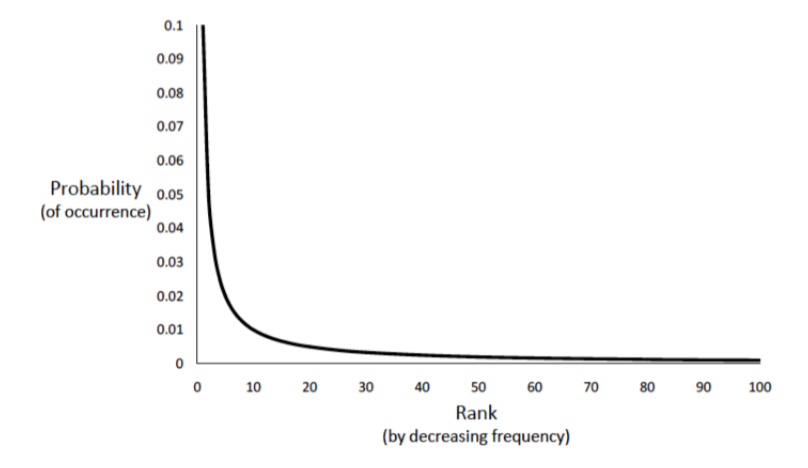
\includegraphics[width=0.55\linewidth]{images/l3-zipf}
\caption{Rango rispetto la probabilità di occorrenza assumendo valida la legge di Zipf con $c = 0.1$}\label{fig:zipf}
\end{figure}

\subsection{Indicazioni di H.P. Luhn}

L'idea per l'indicizzazione è quindi quella di definire due soglie di \textit{cut-off} per evitare di prendere in considerazione le parole troppo frequenti, perché poco significative, e quelle troppo poco, per limitare l'effetto degli errori di battitura.

Ogni parola ha un certo \textbf{resolving power}, ovvero una certa capacità di discriminare il contenuto del documento da quello degli altri e di caratterizzare il contenuto della collezione.

\begin{figure}[htbp]
	\centering
	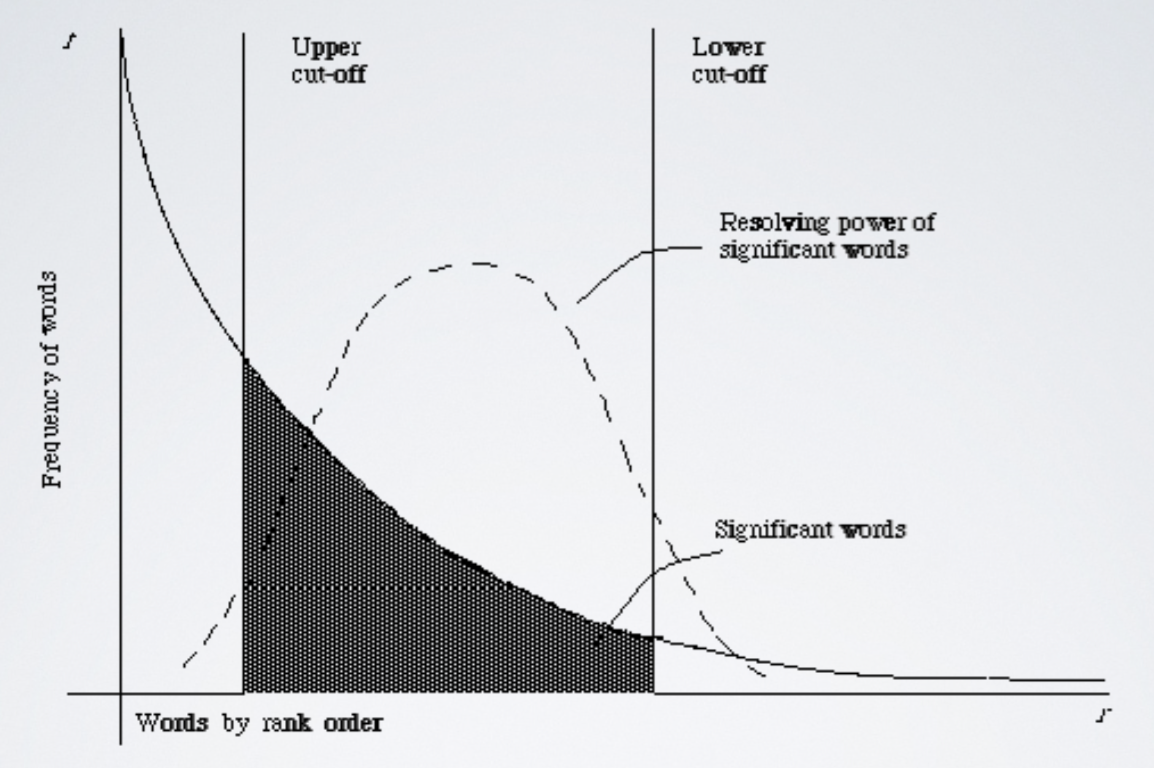
\includegraphics[width=0.55\linewidth]{images/l3-cutoff}
	\caption{Plot della curva $r \times f$ che evidenzia la posizione delle parole significative.}
\end{figure}

Questo vale per le collezioni generiche dei documenti, mentre se si parla di un argomento specifico si può dare maggiore peso a determinate parole. Ad esempio può capitare che se viene preso in esame un manuale di MySQL è ovvio che le parole ``MySQL'' e  ``table'' compariranno tante volte anche se non sono articoli.

C'è anche un altro discorso relativo alla forma plurale delle parole, che in conteggio di frequenza viene considerata come una parola diversa, quando in realtà può essere che abbia lo stesso valore informativo della forma singolare. In alcuni casi è quindi opportuno sommare le occorrenze della forma plurale e di quella singolare.

Si ha quindi che i passi per applicare le indicazioni di Luhn sono:

\begin{itemize}
	\item Si calcoli la frequenza di ogni descrittore in ogni documento della collezione di riferimento. C'è inoltre da scegliere come trattare le parti di contorno dei documenti come l'indice, la premessa, ecc. tali parti tipicamente non vengono considerate.
	\item Si calcoli la frequenza totale di ogni descrittore.
	\item Si ordino i descrittori per frequenza decrescente.
	\item Si scelga una soglia di \textit{upper cut-off} e si rimuovano dalla lista i descrittori con frequenza superiore alla soglia. In questo modo si rimuovono gli articoli, le preposizioni, ecc.
	\item Si scelga un'altra soglia di \textit{lower cut-off} e si rimuovano dalla lista i descrittori con frequenza inferiore al valore di soglia. In questo modo si rimuovono i descrittori ``rumore''  o che non apportano alcun contribuito alla descrizione del contenuto.
\end{itemize}

\noindent Entrambe le soglie possono essere calcolate in modo euristico.

Le parole che vengo eliminate dalle soglie di cut-off vengono nominate \textbf{stop word} e sono raccolte nella lista che prende il nome di \textbf{stop list}.


\textbf{{\color{Red} Possibile esercizio:}} Domande relative alle osservazioni proposte da Zipf e Luhn.

\section{Indicizzazione}

L'indicizzazione ha l'obiettivo di rappresentare il contenuto informativo di un documento e nel tempo questo processo ha preso una struttura a fasi.
Il documento viene rappresentato da dei descrittori che vengono utilizzati per la costruzione degli indici utili al reperimento dell'informazione.

Quindi l'indicizzazione fornisce automaticamente una rappresentazione più compatta e direttamente utilizzabile del contenuto informativo del documento. Gli indici sono utilizzati come surrogati del contenuto del documento durante la fase di reperimento.

L'indicizzazione può essere svolta:
\begin{itemize}
	\item manualmente
	\item in modo automatico
	\item in modo semi-automatico, quando è necessario intervenire all'interno del processo per prendere delle decisioni che non possono essere prese in modo automatico.
\end{itemize}

\noindent Tutti questi metodi funzionano estraendo direttamente dal documento le informazioni. Tuttavia possono essere estesi in modo che vengano presi in considerazione anche dei dizionari o delle meta-informazioni.

\begin{figure}[htbp]
	\centering
	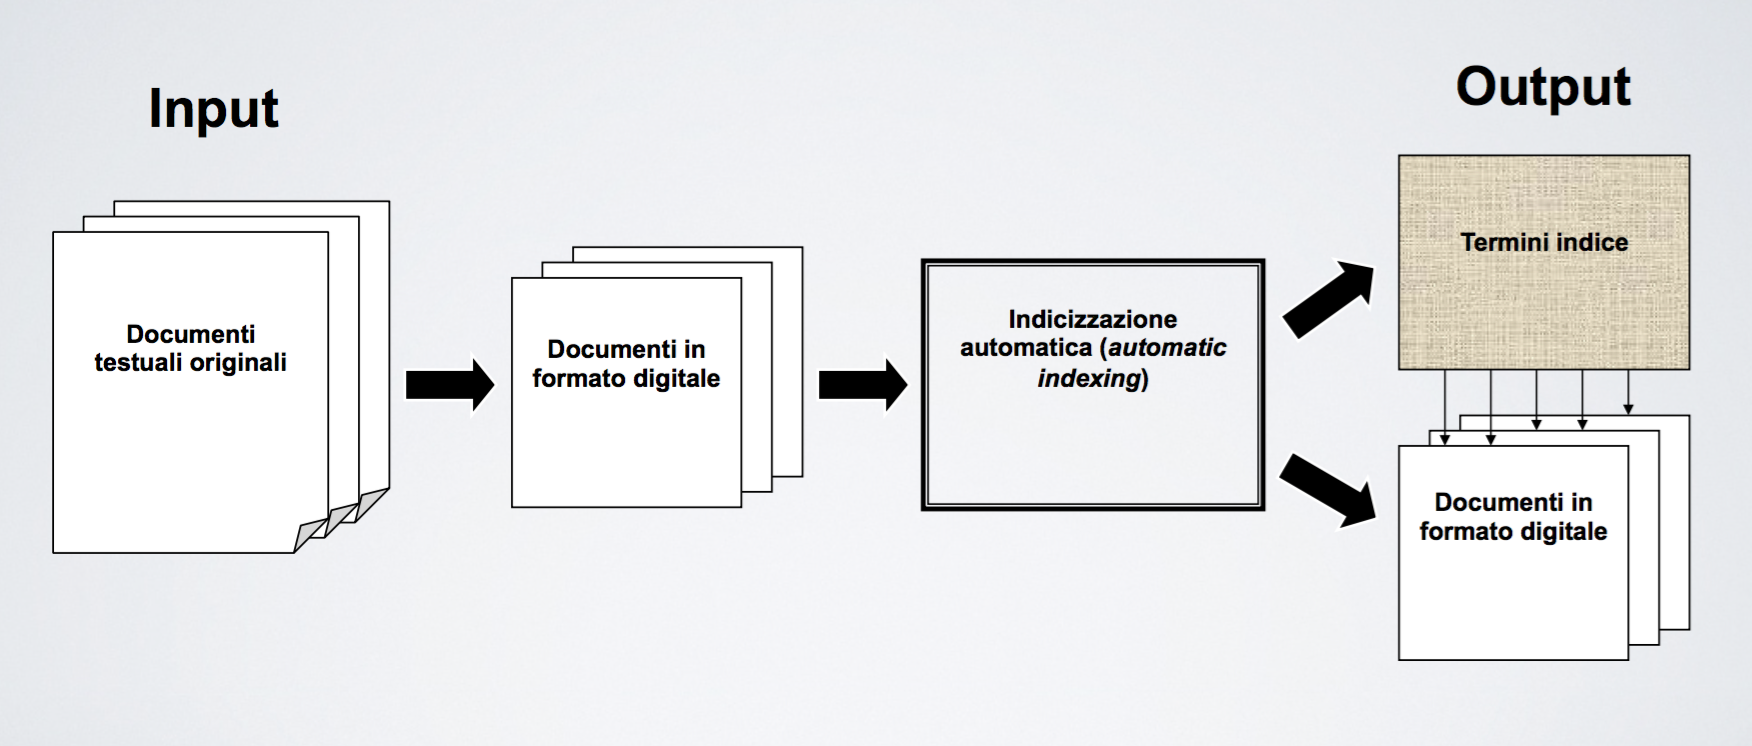
\includegraphics[width=0.7\linewidth]{images/l3-indicizzazione}
	\caption{Schema generale dell'indicizzazione}
\end{figure}

\subsection{Indicizzazione automatica dei testi}

L'indicizzazione automatica di un documento testuale è un processo che esamina automaticamente gli oggetti informativi (parole, frasi, didascalie, figure, ecc.) che compongono il documento e produce una lista di termini indice presenti nell'intera collezione dei documenti.

L'estrazione dei termini indice viene fatta da appositi algoritmi e, una volta estratti, questi vengono collegati ai diversi documenti che li contengono.
Così facendo durante il reperimento sarà sufficiente fare riferimento ai termini indice e non all'intera collezione.

\subsection{Attuazione dell'indicizzazione automatica}

L'indicizzazione automatica dei documenti testuali viene eseguita in più fasi, che devono essere attuate in sequenza:

\begin{enumerate}
	\item Analisi lessicale e selezione delle parole.
	\item Eventuale rimozione delle stop word.
	\item Riduzione delle parole originali alle rispettive radici (\textit{STEM}). Ad esempio le forme plurali vengono ridotte a quelle singolari.
	\item Composizione dei termini. Come ad esempio ``information retrieval''. Ovvero le parole vengono combinate tra loro quando si trovano ad una determinata distanza.
	\item Creazione dell'indice.
	\item Eventuale pesatura degli elementi dell'indice. 
\end{enumerate}

Alla fine di queste fasi l'indice sarà composto da parole, termini e frasi che noi riteniamo significative, assieme alle informazioni del peso che gli diamo e alla loro frequenza all'interno dei documenti.









% !TEX encoding = UTF-8
% !TEX program = pdflatex
% !TEX root = AALP.tex
% !TEX spellcheck = it-IT

% 20 Ottobre 2016
% \section sistemi di tipi
% \subsubsection Teorema di Preservazione (Subject reduction)

% Dimostrazione del lemma di sostituzione (spostata al posto corretto in lezione5)

\subsubsection{Corollario di Subject-reduction}

\begin{center}
	Se $\emptyset \vdash M : T$ e $M \rightarrow^* M'$, allora $\emptyset \vdash M' : T$
\end{center}

\paragraph{Dimostrazione}

La dimostrazione viene fatta per induzione sul numero di passi che da $M$ portano ad $M'$.

Il caso base è quello con il cammino di lunghezza 0, ovvero quando $M = M'$ e la tesi è trivialmente vera.

Nel caso induttivo ho che $M \rightarrow^{*}_k M_1 \rightarrow M'$, pertanto per ipotesi induttiva ho che $\emptyset \vdash M_1 : T$. 

Ho poi che $M_1 \rightarrow M'$ e quindi posso applicare subject-reduction per ottenere che $\emptyset \vdash M' : T$.

\subsubsection{Teorema di Safety - Completo}

\begin{center}
	Se $\emptyset \vdash M : T $ e $M \rightarrow^* M'$ e $M' \not\rightarrow$, allora $M'$ è un valore.
\end{center}

\paragraph{Dimostrazione}

Alle due ipotesi posso applicare il corollario di subject-reduction, ottenendo che $\emptyset \vdash M' : T$.

Per il teorema di progressione ho poi che $M'$ è un valore oppure $M'$ fa un passo e va in $M''$, ma per ipotesi $M'$ non fa un passo e quindi $M'$ è per forza un valore.

\subsection{Esercizio sul typing}

Da notare che nel contesto iniziale non servono giudizi di tipo perché tutte le variabili che compaiono sono all'interno delle funzioni e che, non essendoci informazioni sui tipi, questi sono ignoti e pertanto è necessario fare anche inferenza durante la risoluzione dell'albero.

\begin{prooftree}	
	
	% App-1
	\AxiomC{$\checkmark$ $\textbf{\textit{T}} = \textbf{\textit{T}}_1 \rightarrow \textit{\textbf{T}}_3$}
	\LeftLabel{(\textsc{Var})}
	\UnaryInfC{$y : T, x : T' \vdash y : T_1 \rightarrow T_3$}
	
	% App-2
	\AxiomC{*}
	\LeftLabel{\textsc{(If)}}
	\UnaryInfC{$y : \textbf{\textit{T}}_1\rightarrow \textbf{\textit{T}}_3, x:T' \vdash \text{if true then }x \text{ else }y \: x : T_1$}
	\LeftLabel{\textsc{(App)}}
	\BinaryInfC{$y : T, x: T' \vdash y \: (\text{if true then }x \text{ else }y \: x) : \: T_3$}
	
	\LeftLabel{\textsc{(Fun)}}
	\UnaryInfC{$y : T \vdash \fn x : \textbf{\textit{T'}} . (y \: (\text{if true then }x \text{ else }y \: x)) : \textbf{\textit{T}}_2 = \textbf{\textit{T'}} \rightarrow \textbf{\textit{T}}_3$}
	
	\LeftLabel{\textsc{(Fun)}}
	\UnaryInfC{$\emptyset \vdash \fn y : \textbf{\textit{T}} . \fn x : T' . (y \: (\text{if true then }x \text{ else }x \: y)) : \textbf{\textit{T}} \rightarrow \textbf{\textit{T}}_2$} % T' \rightarrow ?
\end{prooftree}

\noindent Dal ramo sinistro di \textsc{(App)} riesco a chiudere con $T = T_1 \rightarrow T_3$ e quindi riporto l'informazione anche sul ramo destro.
La derivazione continua applicando \textsc{(IfThenElse)} e con $\Gamma = y:T_1 \rightarrow T_3, x:T'$:

\begin{prooftree}
	%if 1
	\AxiomC{$\checkmark$}
	\LeftLabel{\textsc{(True)}}
	\UnaryInfC{$\Gamma \vdash \true : \Bool$}
	
	%if 2
	\AxiomC{$\checkmark$  $\textbf{\textit{T}}_1 = \textbf{\textit{T'}}$}
	\LeftLabel{\textsc{(Var)}}
	\UnaryInfC{$y: T_1 \rightarrow T_3, x:T' \vdash x : T_1$}
	
	%if 3
	\AxiomC{**}
	\LeftLabel{\textsc{(App)}}
	\UnaryInfC{$y : \textbf{\textit{T'}} \rightarrow T_3, x:T' \vdash y \: x : \textbf{\textit{T'}}$}
	% per quello che ho scoperto 
	\UnaryInfC{$y : T_1 \rightarrow T_3, x:T' \vdash y \: x : T_1$}
	\LeftLabel{\textsc{(If)}}
	\TrinaryInfC{(*)$\Gamma \vdash \text{if true then }x \text{ else }y \: x : T_1$}
\end{prooftree}

\noindent Dal ramo centrale della regola \textsc{(IfThenElse)} scopro che $T_1 = T'$ e quindi aggiorno il ramo destro e il contesto, che ora è  $\Gamma = y:T' \rightarrow T_3, x:T'$.

\begin{prooftree}
	\AxiomC{$\checkmark$}
	\LeftLabel{\textsc{(Var)}}
	\UnaryInfC{$y:T' \rightarrow T_3 , x:T' \vdash y : T_4 \rightarrow T'$}
	
	\AxiomC{$\checkmark$}
	\LeftLabel{\textsc{(Var)}}
	\UnaryInfC{$y : T' \rightarrow T_3 , x :T'\vdash x : T_4$}
	
	\LeftLabel{\textsc{(App)}}
	\BinaryInfC{(**)$\Gamma \vdash y \: x : T'$}
\end{prooftree}

\noindent Da quest'ultimo albero trovo che $T' = T_4 = T_3$. Andando a sostituire il tutto trovo che:

\begin{itemize}
	\item $y : T' \rightarrow T'$
	\item $x : T'$
	\item $T_2 = T' \rightarrow T_3 = T' \rightarrow T'$
	\item $T = T_1 \rightarrow T_3 = T' \rightarrow T'$
	\item Il tipo del programma è quindi $(T' \rightarrow T') \rightarrow (T' \rightarrow T')$
\end{itemize}

\chapter{Estensioni del linguaggio funzionale}

\section{Unit}

Nei linguaggi funzionali, ogni funzione deve ritornare sempre un valore, tuttavia può capitare che delle funzioni non debbano ritornare un valore. In questo caso viene ritornato il tipo \text{Unit} che può assumere l'\textbf{unico} \textbf{valore} \texttt{()} o \text{unit}.

Ad esempio la funzione \texttt{print} in Scala ritorna un valore di questo tipo:

\begin{lstlisting}[language=Scala]
def print( x: Any) : Unit = {...}
\end{lstlisting}

\noindent allo stesso modo anche l'assegnamento in Scala ritorna un valore \text{Unit} mentre in C/C++ viene solitamente ritornato il valore assegnato (per concatenare le operazioni di assegnamento).

Aggiungere \text{Unit} al linguaggio vuol dire estendere la definizione:

\begin{align*}
	M &::= \ldots \: | \: \text{unit} \: | \: \ldots \\
	v &::= \ldots \: | \: \text{unit} \: | \: \ldots \\
	T &::= \ldots \: | \: \text{Unit} \: | \: \ldots 
\end{align*}

\noindent e allo stesso modo serve una regola di tipo:

\begin{prooftree}
	\AxiomC{}
	\LL{Unit}
	\UnaryInfC{$\Gamma \vdash \text{unit : Unit}$}
\end{prooftree}

\noindent La killer-feature del tipo \text{Unit} è la possibilità di implementare il call-by-name utilizzando il call-by-value.

Ad esempio, tornano alle nostre asserzioni in Scala

\begin{lstlisting}[language=Scala, caption=Version ``standard'' delle asserzioni]
var assEnabled = true
...
def assert(pred : Bool) = 
	if (assEnabled && !pred)
		throw Exc
...

assert(saldoConto() > 0)
\end{lstlisting}


\noindent possiamo utilizzare \text{Unit} per far funzionare il codice precedente come se fosse call-by-name ma senza specificarlo:

\begin{lstlisting}[language=Scala, caption=Version ``standard'' delle asserzioni]
var assEnabled = true
...
def assert(pred : Unit => Bool) = 
	if (assEnabled && pred() == false) /** l'invocazione con () passa Unit*/
		throw Exc
...
assert(fn x:Unit . (saldoConto() > 0) ) /** pseudo scala */
assert( () =>  (saldoConto() > 0) ) /** sintassi corretta (la funzione anonima non ha parametri) */
\end{lstlisting}

\noindent In questo caso con la sintassi call-by-value viene calcolato il valore del parametro, ma in questo caso il parametro è una funzione che è già un valore.
Quindi, se le asserzioni sono disabilitate, alla chiamata della funzione \texttt{assert} non viene chiamata la funzione \texttt{saldoConto()} perché la funzione è già un valore.

Per riportare la stessa cosa nel nostro linguaggio funzionale con il call-by-value:

$$
\fn x:T.M \: N \rightsquigarrow \: \big(\fn y : \text{Unit} \rightarrow T . M\{x := y \: \text{unit}\} \big) \:\:  \big(\fn z : \text{Unit} . N \big)
$$

\subsection{Implementazione del while}

Vogliamo definire una funzione che si comporta come il while in Scala.

\begin{lstlisting}[language=Scala, caption=I parametri devono essere dichiarati come call-by-name oppure  ]
def WHILE(cond : =>Bool , command : =>Unit ) : Unit = 
	if (cond == false ) () /** In scala il return è opzionale, () è il valore di Unit*/
	else {
		command
		WHILE(cond, command)
	}

/** Uso della funzione */
var a = 0
WHILE(a < 4 , {print(a); a=a+1})
\end{lstlisting}

\noindent Dato che sono in call-by-value i parametri vengono valutati prima di invocare per la prima volta il while, quindi o li passo per by-name oppure li passo utilizzando una funzione. 
Questo perché sia il codice del corpo che la condizione devono poi essere rieseguiti (valutati) nelle successive iterazioni. 



\chapter{Il modello lineare nei parametri}

\textbf{Problema di riferimento:} come il prezzo influenza il consumo di
gas? Si hanno a disposizione le informazioni relative alla domanda di
gas e al prezzo dello stesso per 20 città in Texas.

Si vuole riuscire a capire se c'è una correlazione tra le due cose.

\begin{figure}[htbp]
	\centering
	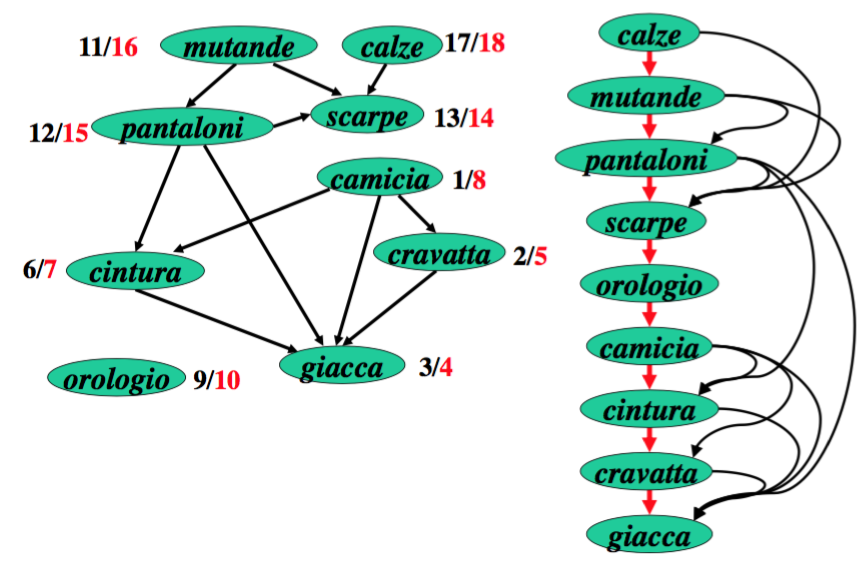
\includegraphics[width=.5\textwidth]{./notes/immagini/l7-fig1.png}
\end{figure}

\section{Un primo modello lineare}\label{un-primo-modello-lineare}

Ipotizzando che ci sia una relazione lineare è possibile utilizzare il
modello del capitolo precedente:

$$
y = \alpha + \beta x + \epsilon
$$

$$
\hat{\beta} = \frac{\cov(X,Y)}{\var(X)} \qquad \hat{\alpha} = \bar{y} - \hat{\beta}\bar{x}
$$

Utilizzando l'ambiente R si ottengono delle informazioni relative all
modello ottenuto:

\begin{verbatim}
lm(formula = gas ~ prezzo)
Residuals:
    Min      1Q  Median      3Q     Max
-40.625 -10.719  -1.136  14.073  38.292
Coefficients:
            Estimate Std. Error t value Pr(>|t|)
(Intercept)  138.561     13.552  10.225 6.34e-09 ***
prezzo        -1.104      0.202  -5.467 3.42e-05 ***
---
Signif. codes:  0 ‘***’ 0.001 ‘**’ 0.01 ‘*’ 0.05 ‘.’ 0.1 ‘ ’ 1
Residual standard error: 20.86 on 18 degrees of freedom
Multiple R-Squared: 0.6241,     Adjusted R-squared: 0.6033
F-statistic: 29.89 on 1 and 18 DF,  p-value: 3.417e-05
\end{verbatim}

Dai dati si può notare che l'indice $ R^2 $ è uguale a 0.62, il che indica un buon andamento lineare.
Inoltre come \textit{p-value} si ottiene un valore molto basso, il che porta a rifiutare l'ipotesi nulla.

Tracciando però i grafici dei residui è possibile osservare c'è una componente indipendente che non è lineare.

\begin{figure}[htbp]
	\centering
	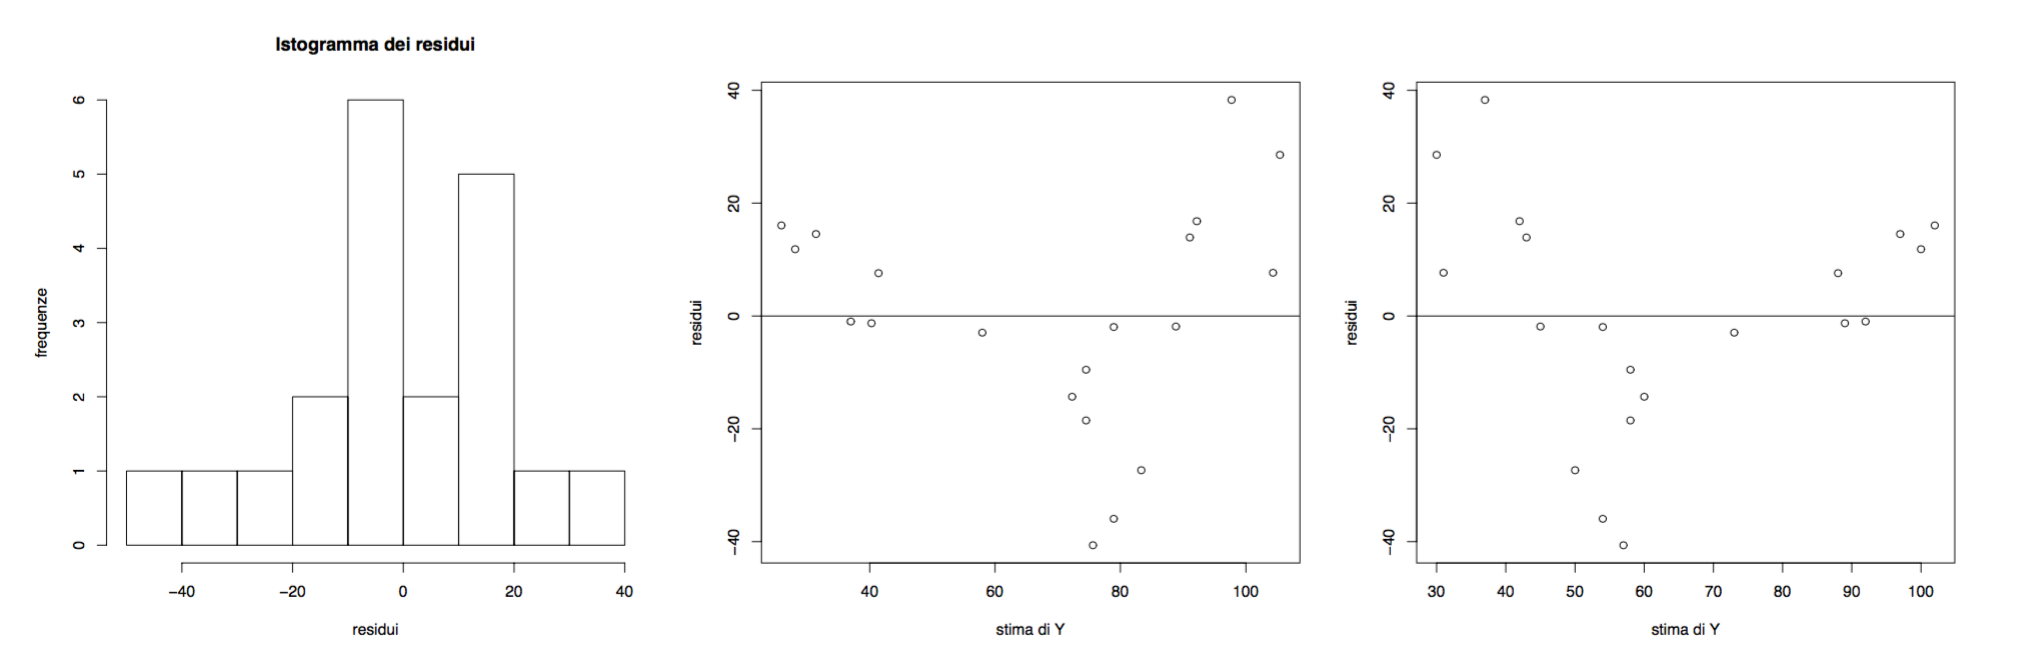
\includegraphics[width=1\textwidth]{./notes/immagini/l7-fig2.png}
	\caption{Tracciamento dei residui per il primo modello. \`{E} possibile notare la presenza di indipendente.}
\end{figure}

\section{Considerazioni sul problema e un secondo modello}\label{considerazioni-sul-problema-e-un-secondo-modello}

Considerando il problema modellato è possibile fare alcune osservazioni:

\begin{itemize}
	\item il consumatore potrebbe destinare solamente un determinato budget $ \kappa $ per l'acquisto del gas, ovvero $ x \cdot y = \kappa $.
	\item è ragionevole pensare che il consumatore debba consumare una quantità minima di gas $ \gamma $
	\item essendo il mercato del gas regolamentato, c'è un prezzo minimo di $ 7 $ centesimi al metro cubo sotto il quale non è possibile vendere il gas.
\end{itemize}

Tenendo in considerazione quanto elencato si arriva ad avere l'equazione:

$$
(x-7)(y-\gamma) = \kappa
$$

la quale può essere riscritta in un modo più simile a quella del modello lineare

$$
y = \gamma + \kappa \cdot \frac{1}{x-7}
$$

e sostituendo la variabile \textit{x} con $ z = \frac{1}{x-7} $, si ottiene proprio la stessa equazione la quale permette di calcolare la retta ai minimi quadrati.

Questo è possibile perché quello che finora è stato chiamato modello lineare è un caso particolare dei \textbf{modelli lineari nei parametri}. Ovvero la limitazione data dalla linearità non riguarda le variabili, ma riguarda solamente i \textbf{parametri} del modello.

Quando viene utilizzato il metodo dei minimi quadrati con questi modelli è necessario tenere in considerazione le trasformazioni che vengono fatte alle variabili, perché i valori calcolati ai minimi quadrati riguardano le variabili trasformate e non quelle di partenza, è necessario quindi \textbf{scalare} in modo opportuno i valori\footnote{Se viene scalata solamente la $ x $ non c'è questo problema perché i minimi quadrati considerano solamente le distanze rispetto l'asse $ y $.}.

La formulazione più generale del modello lineare è quindi

$$
g(y) = \alpha + \beta h(x) + \epsilon
$$

Il modello ottenuto per la nuova formulazione è:
\begin{verbatim}
lm(formula = gas ~ I(1/(prezzo - 7)))
Residuals:
Min    1Q  Median  3Q    Max
-29.617 -4.574 2.394 7.800 30.917
Coefficients:
Estimate Std. Error t value Pr(>|t|) 
(Intercept) 3.918 8.376 0.468 0.646
I(1/(prezzo - 7)) 3034.938 357.037 8.500 1.02e-07 *** 
---
Signif. codes: 0 ‘***’ 0.001 ‘**’ 0.01 ‘*’ 0.05 ‘.’ 0.1 ‘ ’ 1
Residual standard error: 15.19 on 18 degrees of freedom 
Multiple R-Squared: 0.8006, Adjusted R-squared: 0.7895 
F-statistic: 72.26 on 1 and 18 DF, p-value: 1.022e-07
\end{verbatim}

ovvero la retta

$$
y = 3.918 + 3034.938 \cdot \frac{1}{x-7}
$$

\begin{figure}[htbp]
	\centering
	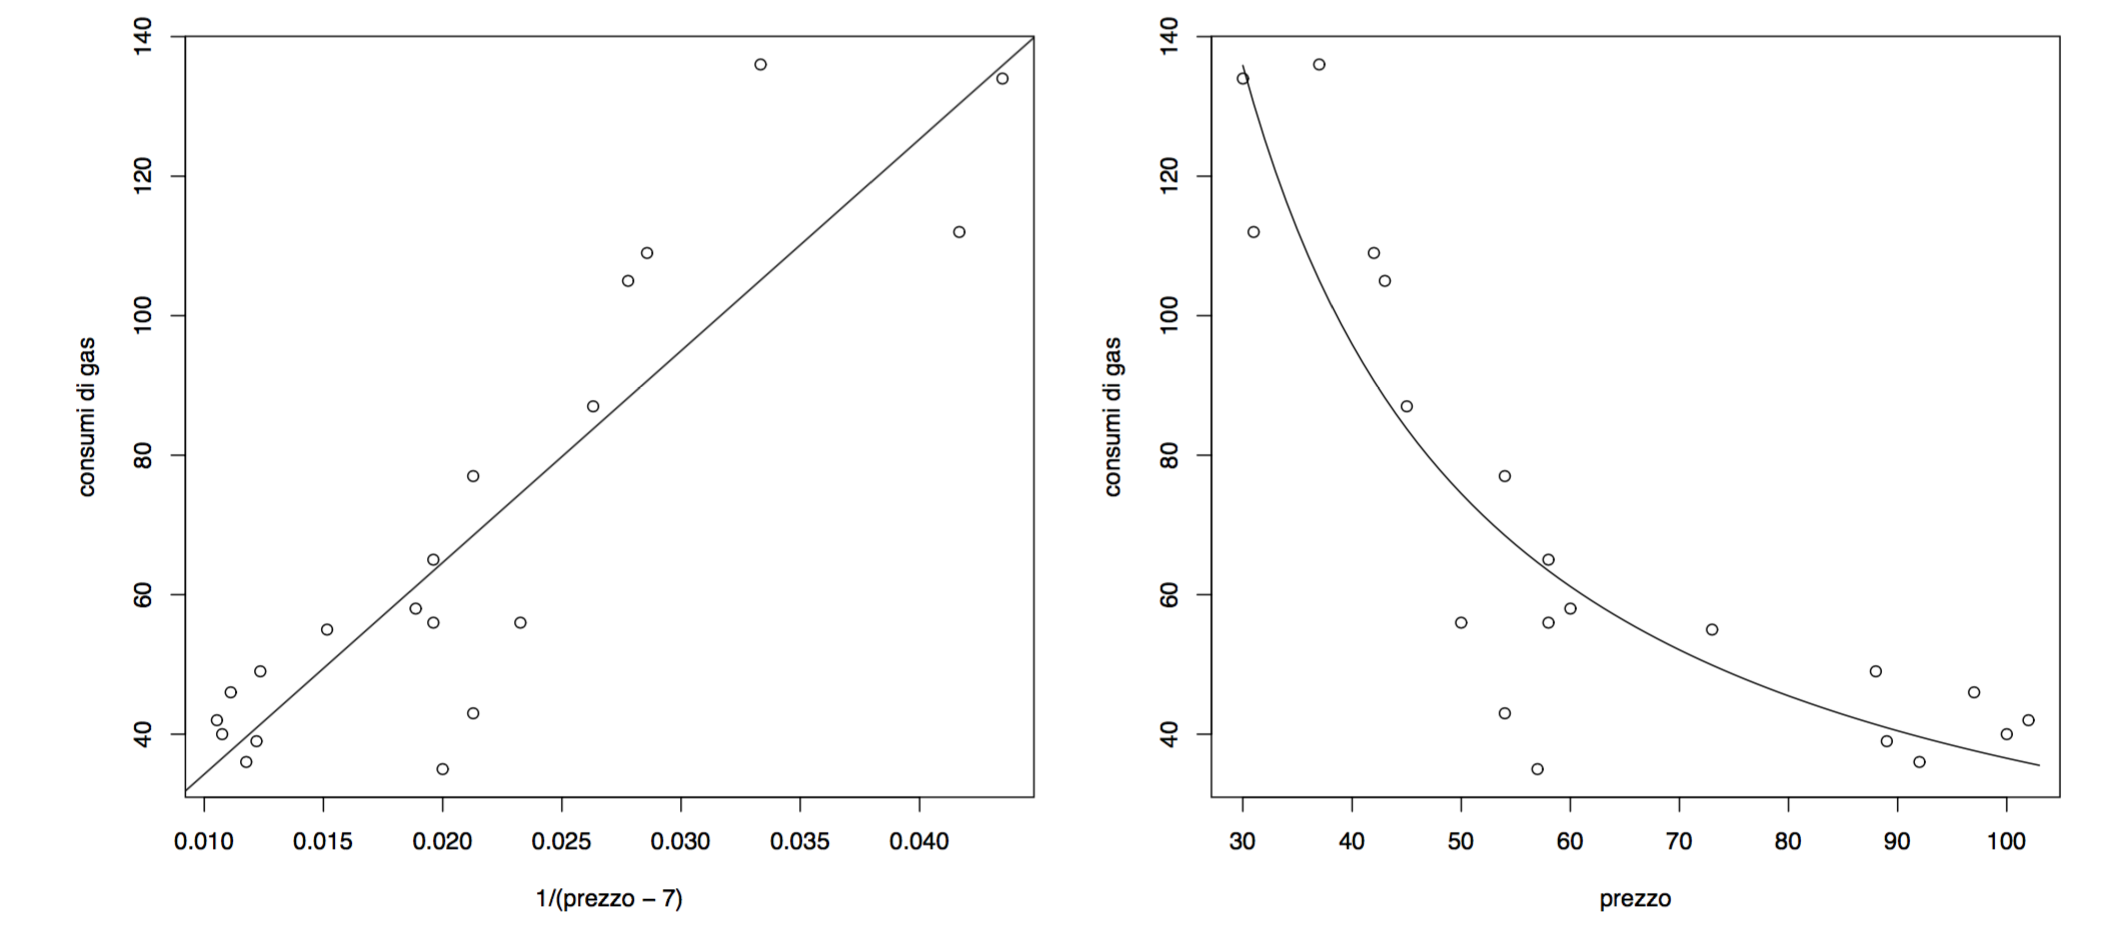
\includegraphics[width=1.1\textwidth]{./notes/immagini/l7-fig3.png}
	\caption{A destra la retta rispetto $ z $. A sinistra il modello lineare tracciato rispetto $ x $.}
\end{figure}

Dai dati del nuovo modello è possibile osservare che la varianza residua (\texttt{Residual standard error} elevato al quadrato) è passata da circa 391 a circa 207, ovvero il quadrato degli errori di previsione è stato ridotto di quasi il $ 50\% $.
Lo stesso effetto può essere visto utilizzando $ R^2 $ che da 0.6241 passa a 0.8006.

\begin{figure}[htbp]
	\centering
	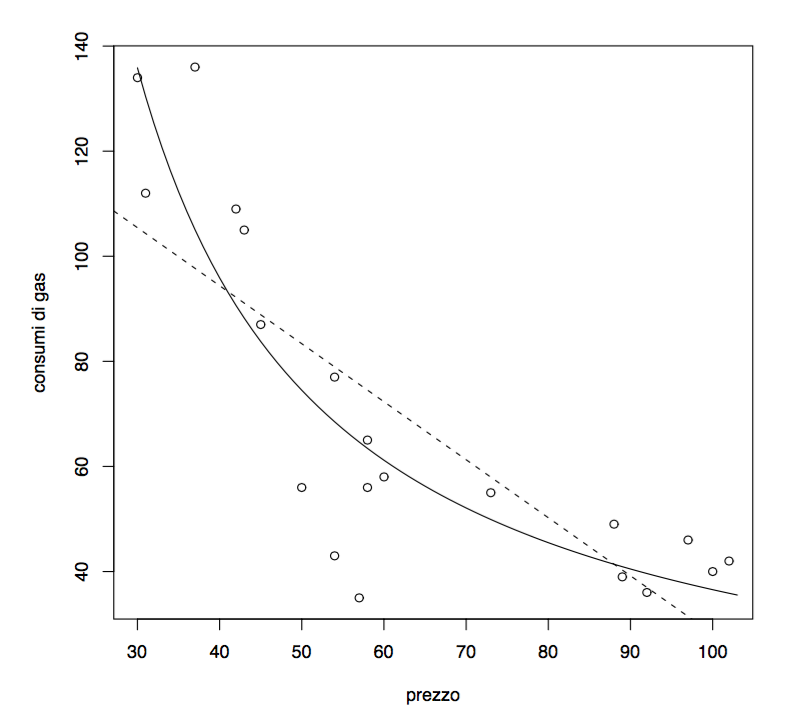
\includegraphics[width=.6\textwidth]{./notes/immagini/l7-fig4.png}
	\caption{Confronto grafico tra i due modelli.}
\end{figure}

\FloatBarrier
\section{Modello lineare con trasformate}\label{modello-lineare-con-trasformate}

\textit{Cambia il dataset di riferimento}, si vuole controllare se il reddito nazionale influisce sulla speranza di vita media dello stato. 

\begin{figure}[htbp]
	\centering
	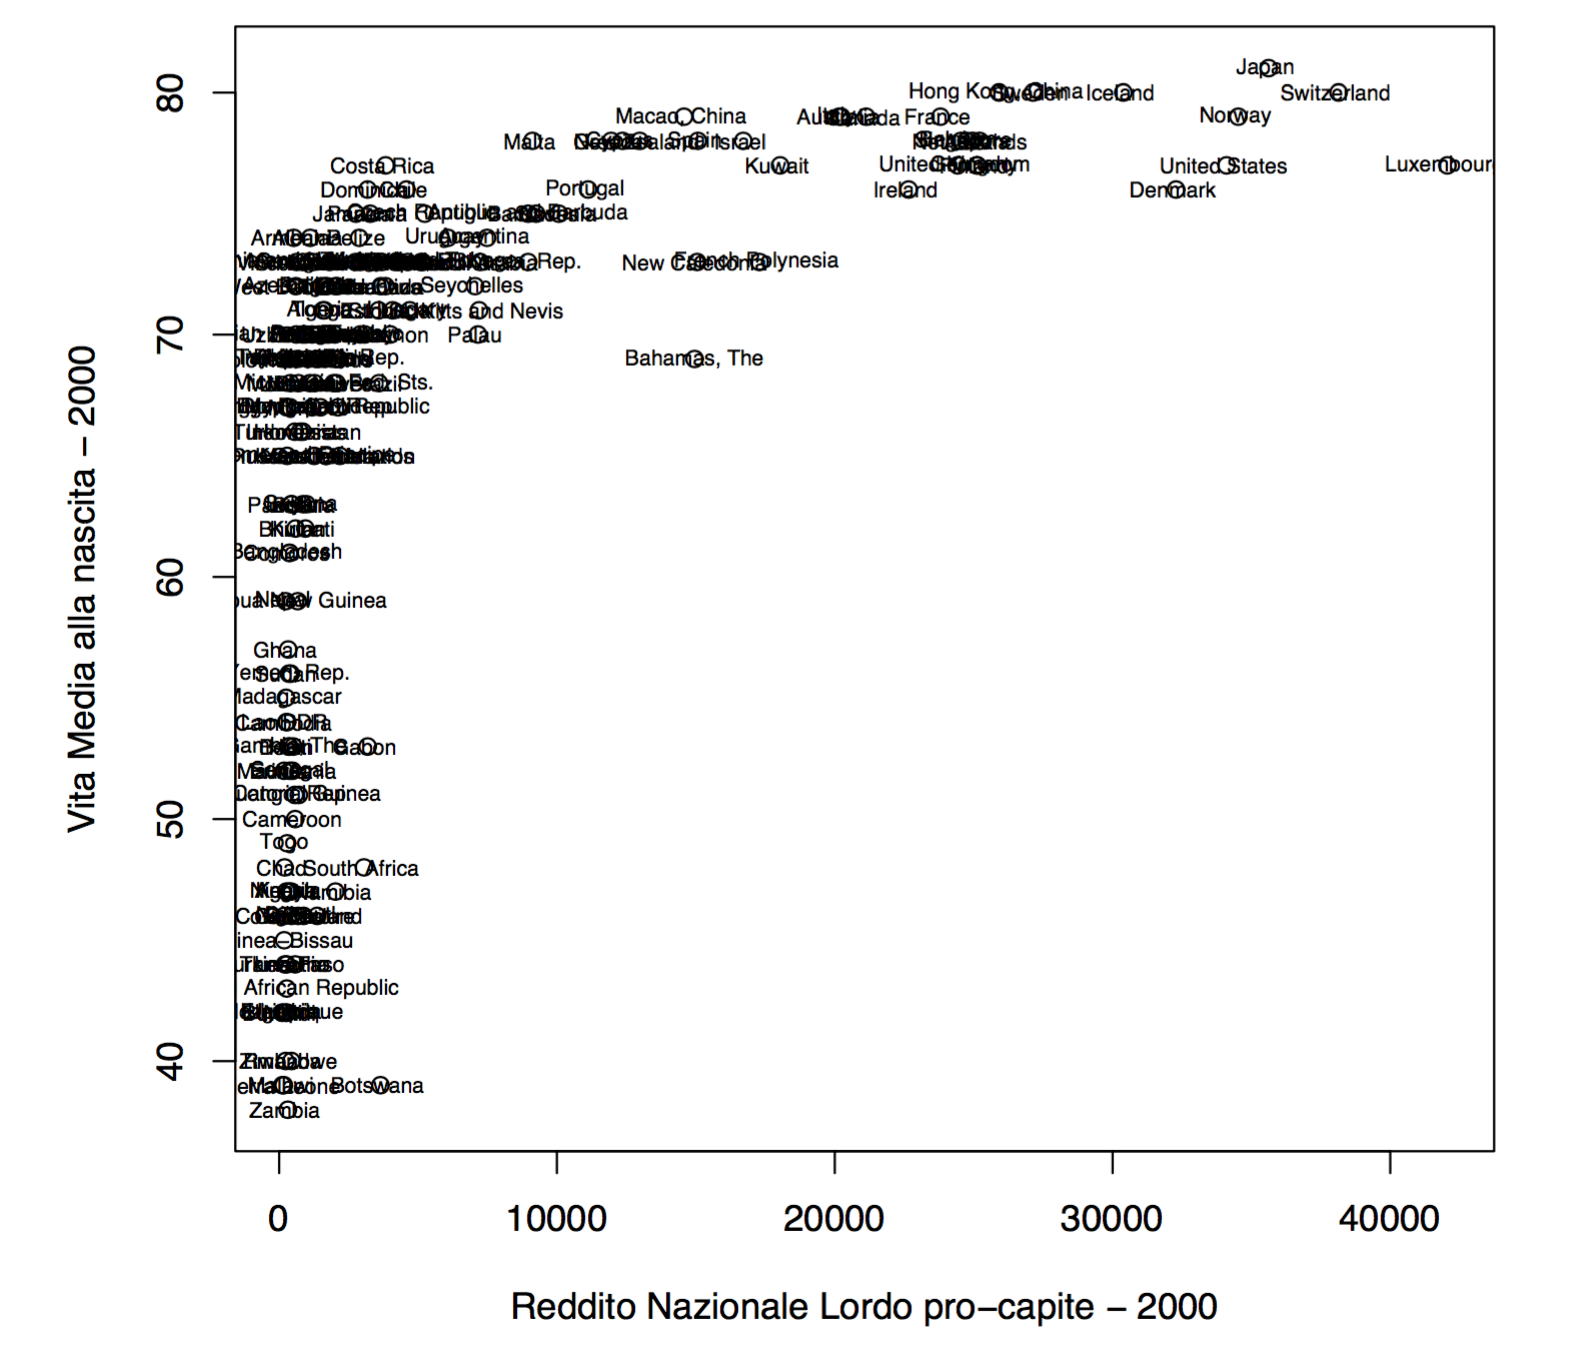
\includegraphics[width=.7\textwidth]{./notes/immagini/l7-fig5.png}
	\caption{Dataset - GNI - ELF}
\end{figure}

La prima cosa da fare è osservare come si comporta il modello lineare senza trasformazioni:

\begin{verbatim}
	lm(formula = elf ~ GNIpc)
	Residuals:
	Min    1Q  Median  3Q    Max
	-24.924 -7.512 4.119 7.431 12.948
	Coefficients:
	Estimate Std. Error t value Pr(>|t|)
	(Intercept) 6.133e+01 8.967e-01 68.390 < 2e-16 ***
	GNIpc 7.115e-04 8.230e-05 8.645 3.76e-15 ***
	---
	Signif. codes: 0 ‘***’ 0.001 ‘**’ 0.01 ‘*’ 0.05 ‘.’ 0.1 ‘ ’ 1
	Residual standard error: 9.903 on 171 degrees of freedom 
	Multiple R-Squared: 0.3041, Adjusted R-squared: 0.3 
	F-statistic: 74.73 on 1 and 171 DF, p-value: 3.757e-15
\end{verbatim}

Si può notare come l'indice $ R^2 $ sia molto basso (0.3041), ma risulta essere molto significativo perché, per il \textit{p-value} ottenuto sia ha che è improbabile che valga l'ipotesi nulla.

Tracciando il modello e il grafico dei residui è possibile notare che
\begin{itemize}
	\item La retta ottenuta non curva abbastanza e quindi non si adatta bene ai dati
	\item Il modello prevede una vita media che può essere maggiore di 90 anni, il che è abbastanza improbabile.
\end{itemize}

\begin{figure}[htbp]
	\centering
	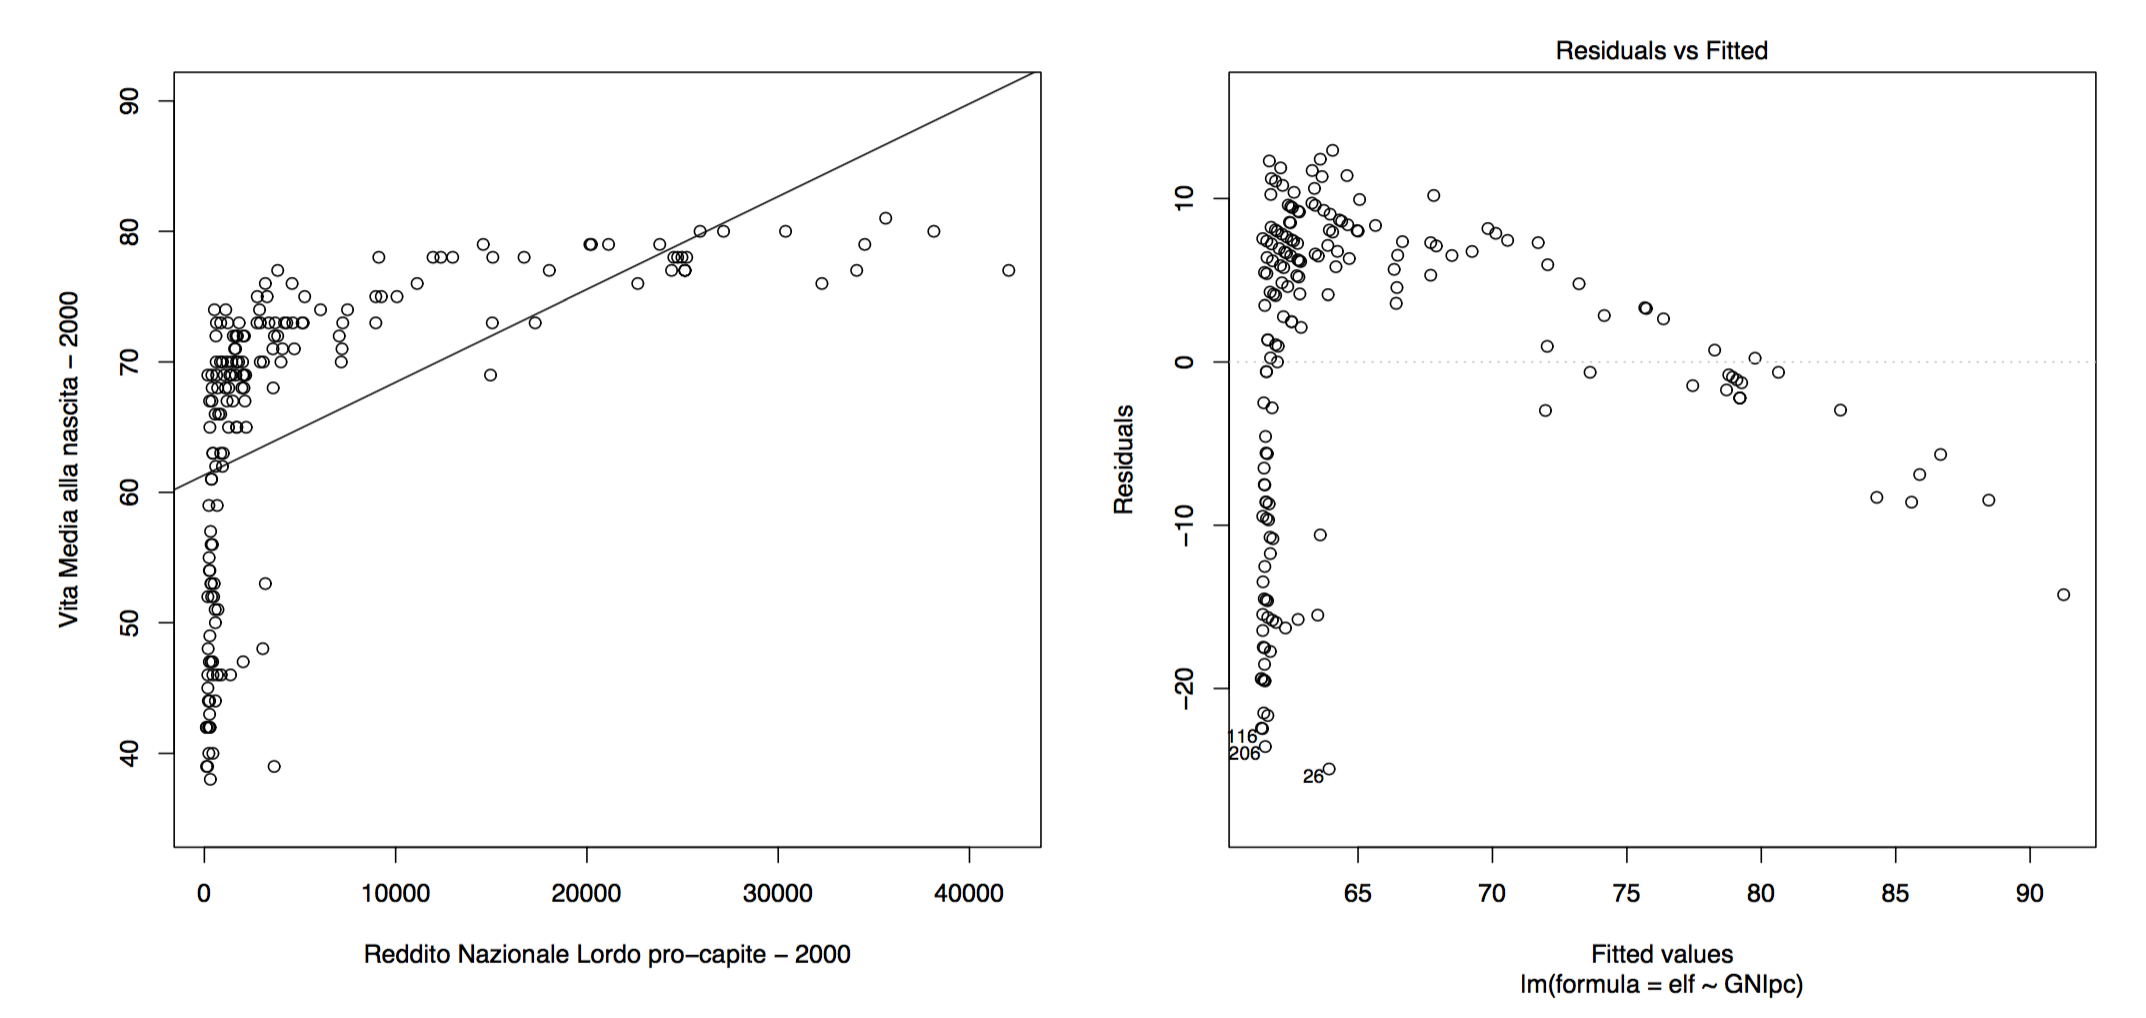
\includegraphics[width=.9\textwidth]{./notes/immagini/l7-fig6.png}
	\caption{Primo modello e residui ottenuti}
\end{figure}

Per adattare meglio la curva è possibile utilizzare la scala logaritmica per l'asse delle \textit{x}. In questo modo, al crescere del reddito viene dato via via meno peso.
Inoltre, rappresentando graficamente questa trasformazioni si ottiene una nuvola di punti più simile ad una retta.

\begin{figure}[htbp]
	\centering
	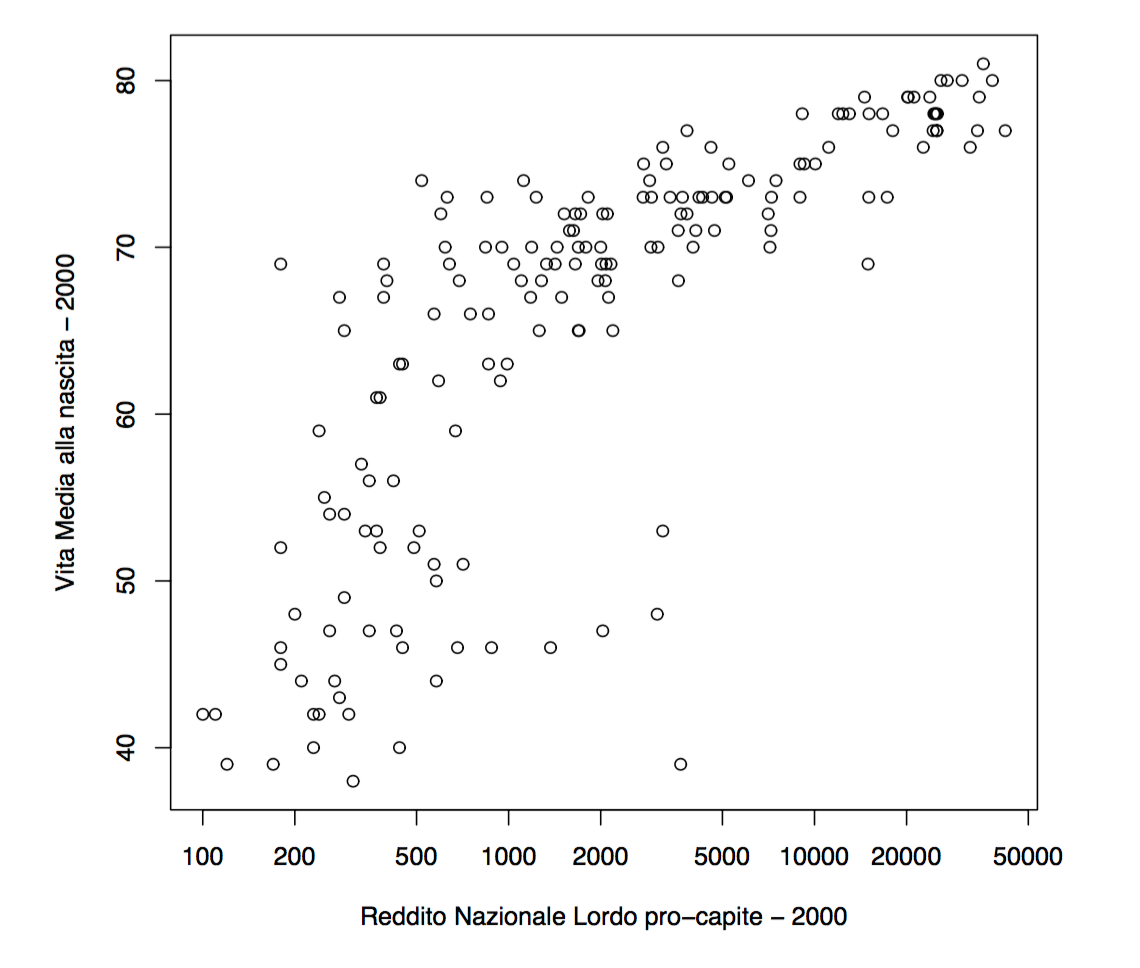
\includegraphics[width=.6\textwidth]{./notes/immagini/l7-fig7.png}
	\caption{Grafico che utilizza la scala logaritmica per i valori delle $ x $. L'asse è comunque etichettato con i valori originali.}
\end{figure}

Il modello diventa quindi

$$
(\text{vita media alla nascita}) = \alpha + \beta \log(\text{reddito nazionale pro capite})
$$

\begin{verbatim}
lm(formula = elf ~ I(logGDP), data = elf.data)
Residuals:
Min     1Q   Median   3Q     Max
-29.6591 -2.9511 0.7906 5.1050 17.4844
Coefficients:
Estimate Std. Error t value Pr(>|t|)
(Intercept) 22.6701 2.8447 7.969 2.02e-13 *** 
I(logGDP) 5.6767 0.3677 15.438 < 2e-16 ***
---
Signif. codes: 0 ‘***’ 0.001 ‘**’ 0.01 ‘*’ 0.05 ‘.’ 0.1 ‘ ’ 1
Residual standard error: 7.674 on 174 degrees of freedom 
Multiple R-Squared: 0.578, Adjusted R-squared: 0.5756 
F-statistic: 238.3 on 1 and 174 DF, p-value: < 2.2e-16
\end{verbatim}

Con questo secondo modello si ottiene un indice $ R^2 $ doppio rispetto al precedente e questo può essere osservato anche nella rappresentazione grafica del nuovo modello.

\begin{figure}[htbp]
	\centering
	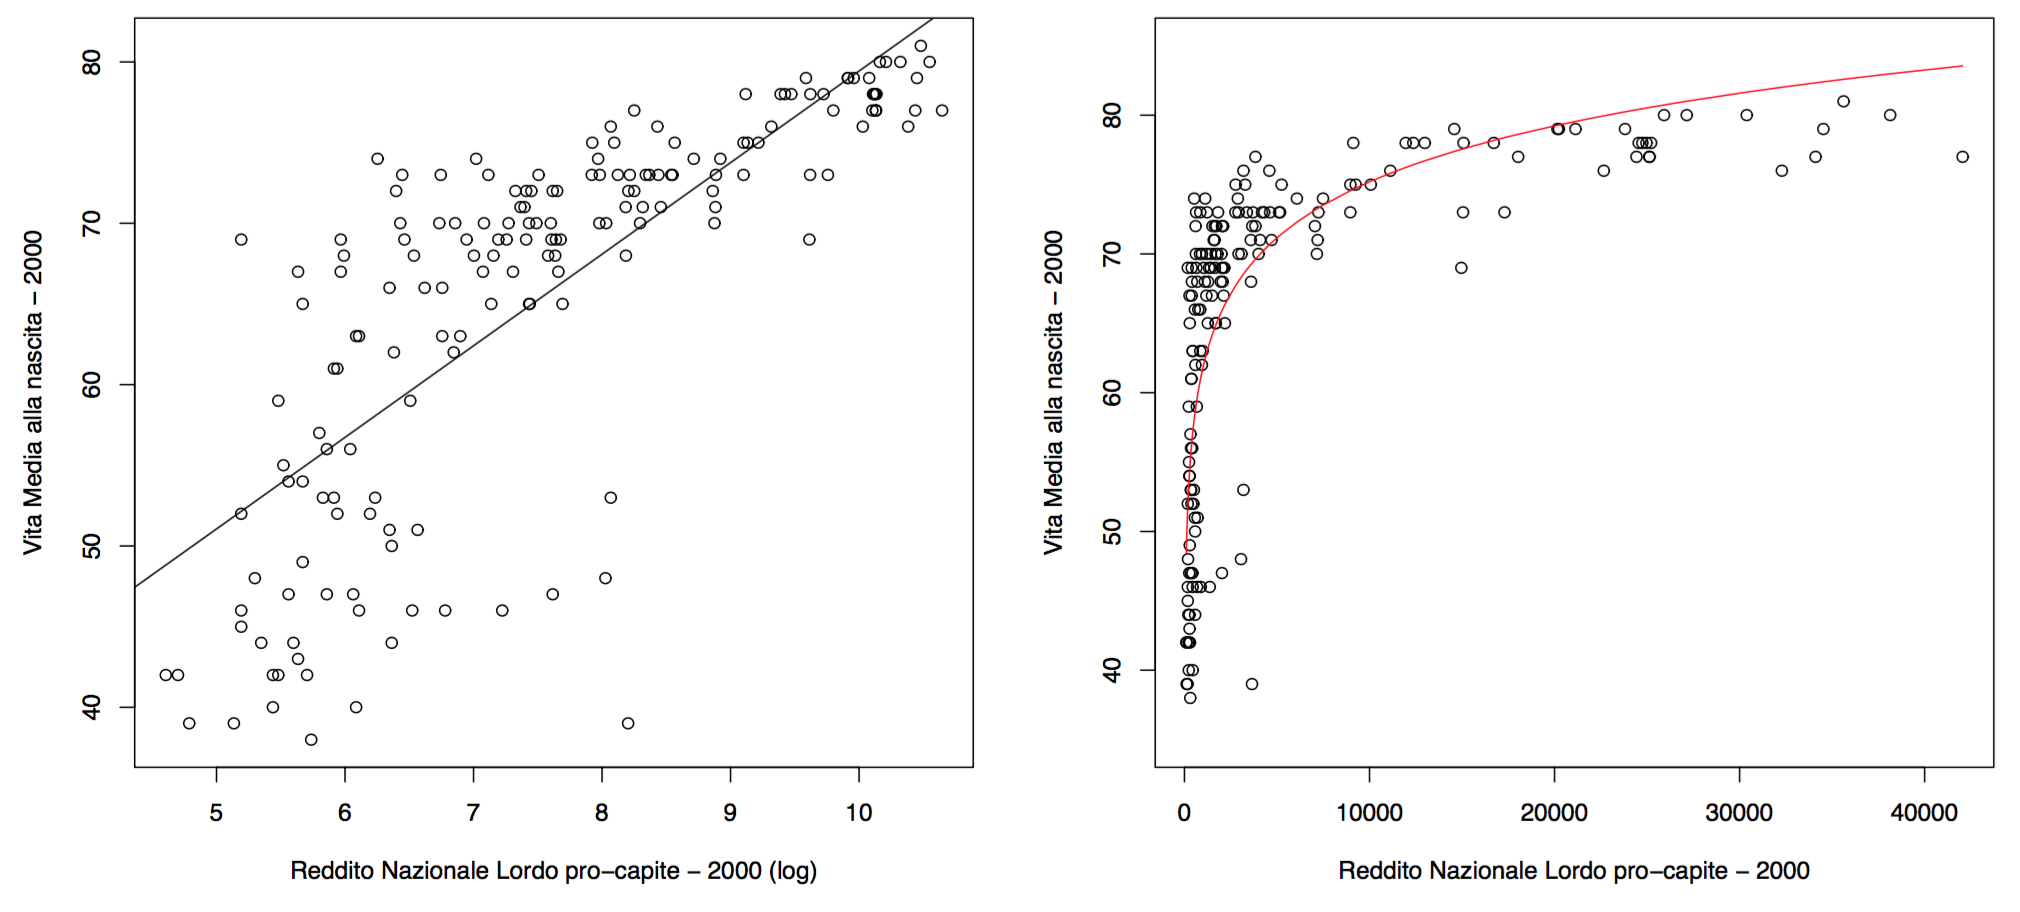
\includegraphics[width=.9\textwidth]{./notes/immagini/l7-fig8.png}
	\caption{Secondo modello: a sinistra con la scala logaritmica, a destra normale.}
\end{figure}

C'è però ancora un problema che riguarda i valori estremi che non vengono approssimati bene dalla curva e lo si può notare anche dai residui.

\begin{figure}[htbp]
	\centering
	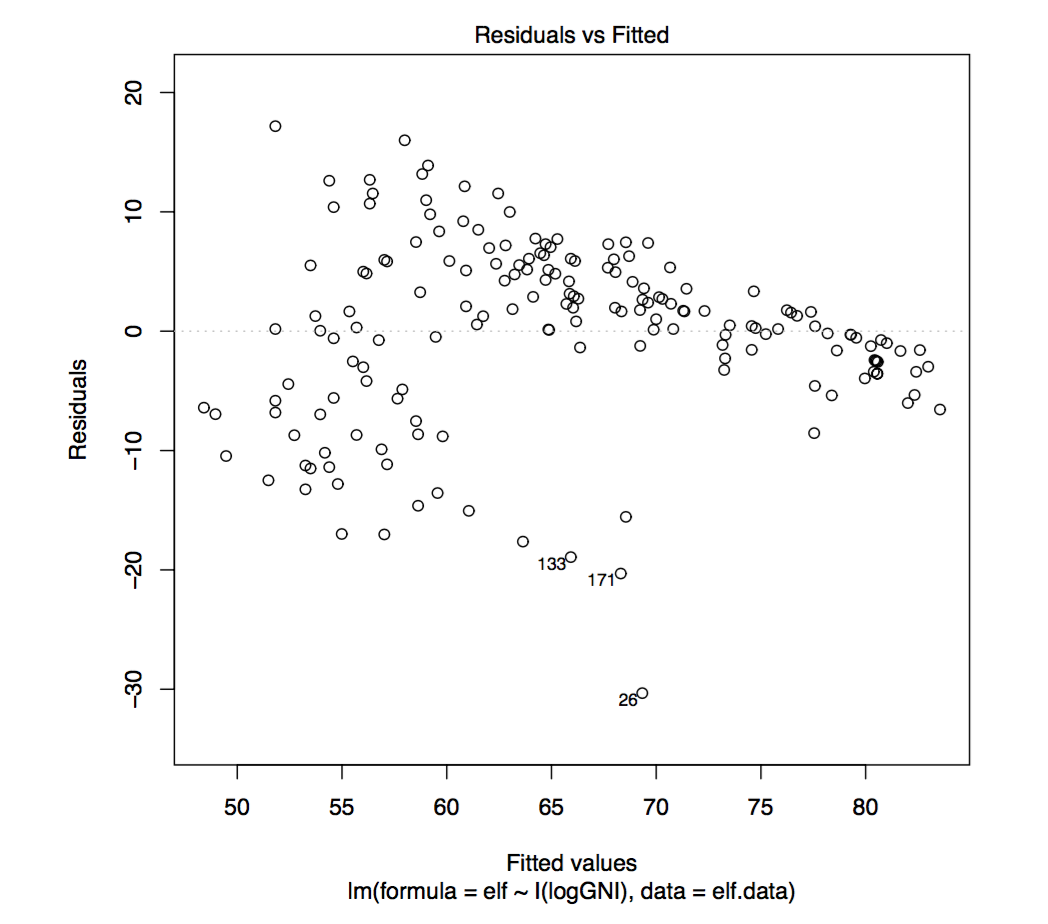
\includegraphics[width=.6\textwidth]{./notes/immagini/l7-fig9.png}
	\caption{Residui per il secondo modello }
\end{figure}

Un'ulteriore modifica può essere quella di trasformare anche la variabile risposta, elevandola alla quinta, in modo da dare maggior peso ai valori maggiori.

Il modello ottenuto è quindi dato da

$$
(\text{vita media alla nascita})^5 = \alpha + \beta \log(\text{reddito nazionale pro capite}) + \epsilon
$$

Da notare che con questa formulazione le ipotesi sugli errori (media nulla, varianza costante, distribuzione normale, ecc.) \textbf{devono valere per gli errori su scala trasformata}.

Una volta calcolato il modello si ottiene

\begin{verbatim}
lm(formula = elf.5 ~ logGNI, data = elf.data)
Residuals:
Min        1Q        Median    3Q       Max
-1.801e+09 -2.817e+08 7.965e+06 3.036e+08 1.334e+09
Coefficients:
Estimate Std. Error t value Pr(>|t|) 
(Intercept) -2.345e+09 1.832e+08 -12.80 <2e-16 *** 
logGNI 5.164e+08 2.376e+07 21.73 <2e-16 ***
---
Signif. codes: 0 ‘***’ 0.001 ‘**’ 0.01 ‘*’ 0.05 ‘.’ 0.1 ‘ ’ 1
Residual standard error: 4.89e+08 on 171 degrees of freedom 
Multiple R-Squared: 0.7341, Adjusted R-squared: 0.7326 
F-statistic: 472.2 on 1 and 171 DF, p-value: < 2.2e-16
\end{verbatim}

\begin{figure}[htbp]
	\centering
	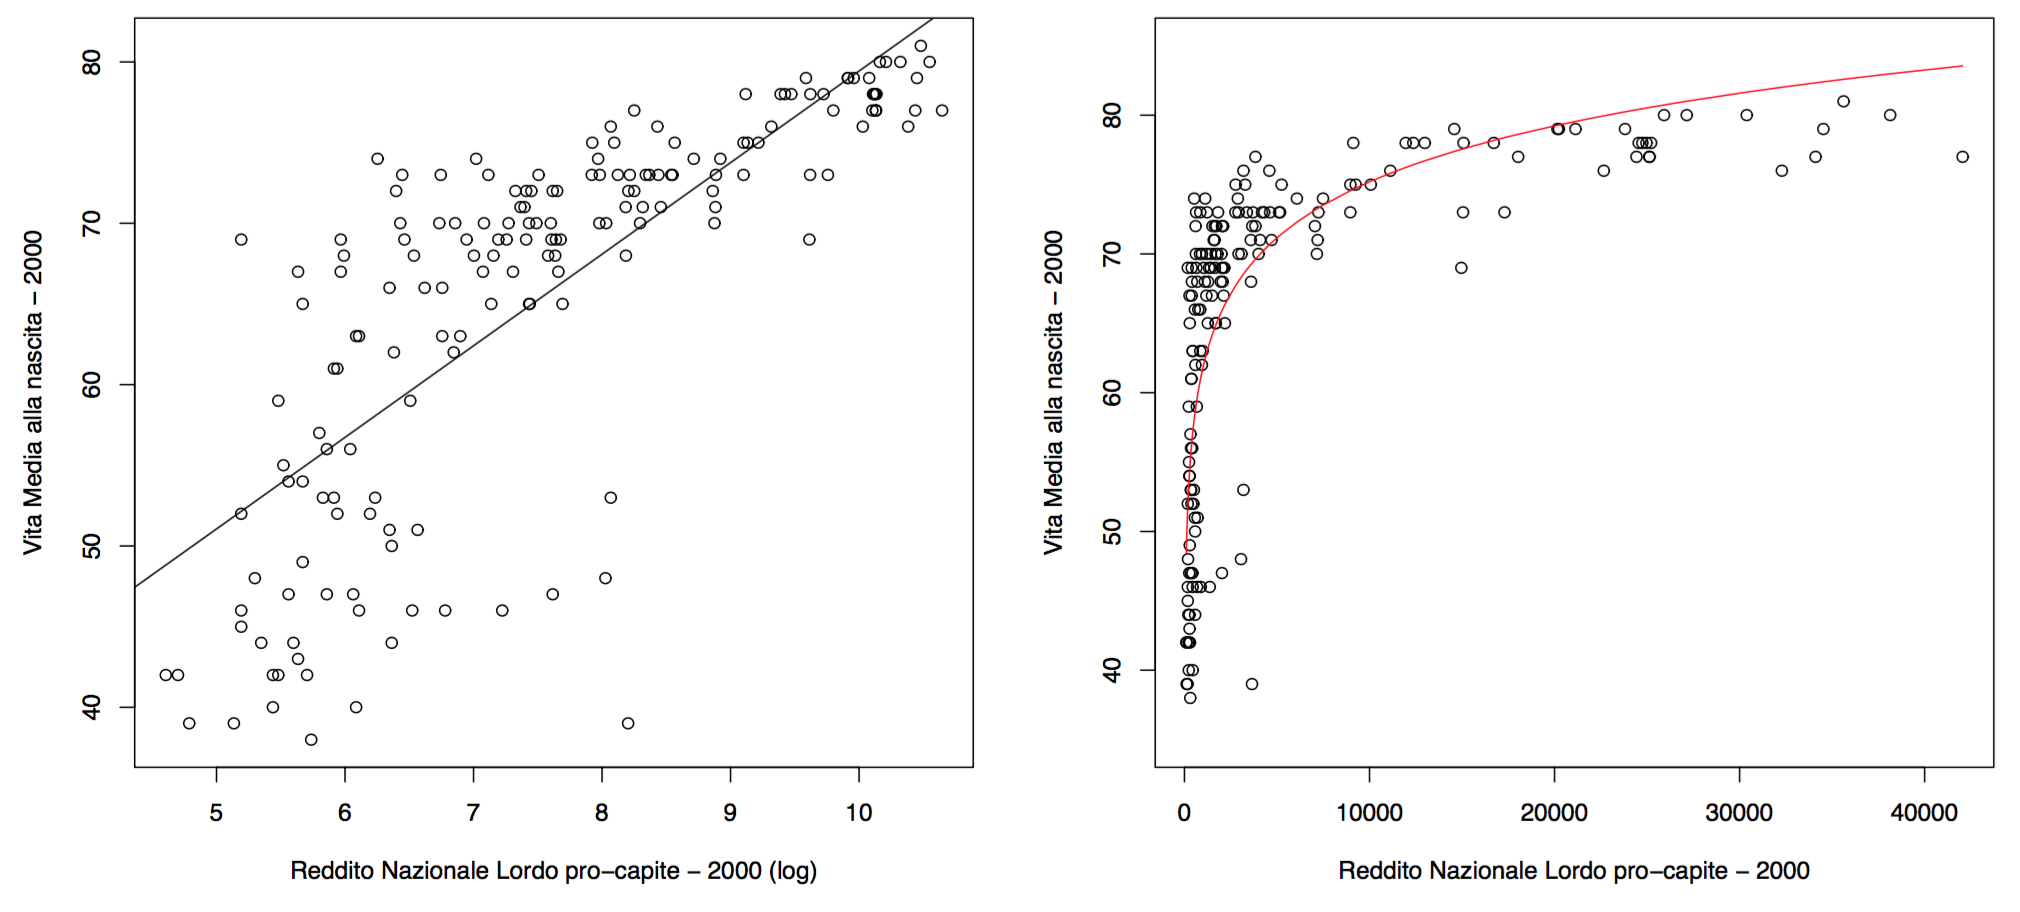
\includegraphics[width=.9\textwidth]{./notes/immagini/l7-fig8.png}
	\caption{Terzo modello: a sinistra con la scala originale e a destra i residui.}
\end{figure}

L'indice $ R^2 $ ottenuto fa riferimento ai residui calcolati sulla scala trasformata, quindi per avere un'indice di adattamento dei dati è possibile utilizzare la media dei quadrati dei residui per la variabile originale:

$$
\frac{1}{n}\sum\limits_{i=1}^n \bigg[ \big(\text{vita media alla nascita}\big)_i - \sqrt[5]{\big(\alpha + \beta \log(\text{reddito nazionale pro capite})_i\big)}\bigg]^2
$$

Calcolando questo valore si ottiene 55.08, mentre con il secondo modello si aveva la varianza dei residui pari a 58.89. Si ottiene quindi una riduzione del $ 6\% $ del quadrato degli errori di previsione.










% !TEX encoding = UTF-8
% !TEX TS-program = pdflatex
% !TEX root = computabilità e algoritmi.tex
% !TEX spellcheck = it-IT
\chapter{Algoritmi su stringhe}\label{algoritmi-su-stringhe}

\section{Il problema del matching esatto}\label{il-problema-del-matching-esatto}

Si ha un pattern \emph{P} di lunghezza \emph{m} e un testo \emph{T} in
cui cercare il pattern di lunghezza $n \geq m$.

Un esempio di problema è la ricerca del pattern \emph{P = aba} in
\emph{T=bbabaxababay}. In questo caso ci sono 3 occorrenze del pattern,
che si sovrappongono tra loro.

Risolvere questo problema in modo efficiente è di importanza chiave dal
momento che tutti i motori di ricerca si basano sul pattern matching
esatto o approssimato. Un altro campo in cui è utile il pattern matching
è nella bioinformatica, infatti, il DNA umano può essere visto come una
stringa di 4 miliardi di caratteri.

\subsection{Notazione utilizzata}\label{notazione-utilizzata}

Una stringa è composta da un insieme $\Sigma$ di simboli
distinguibili e che prendono il nome di \textbf{caratteri dell'alfabeto}.

L'alfabeto, ovvero l'insieme di simboli, può essere finito oppure
infinito ed è dotato di un ordine totale tra i vari simboli.

Una successione finita dei caratteri dell'alfabeto prende il nome di
\textbf{stringa} e i caratteri che la compongono vengono indicizzati a
partire da 1.

$$
X = x_1 \ldots x_n
$$

$|X|$ indica la lunghezza di una stringa e nel
caso questa sia 0, la stringa è vuota e viene rappresentata con
$\epsilon$.

Due stringhe possono essere concatenate tra loro:

$$
X \cdot Y = x_1\ldots x_ny_1\ldots y_m
$$

e $\epsilon$ è l'elemento neutro per la concatenazione, dal momento
che la concatenazione della stringa vuota ad un'altra stringa è uguale
alla stringa di partenza.

La concatenazione multipla della stessa stringa viene indicata con
l'esponenziale:

$$
X^k = \underbrace{X \cdot \ldots \cdot X}_{k}
$$

Una \textbf{sottostringa} di una stringa \emph{X} è una stringa
\emph{Y}, tale che
$X = Z \cdot Y \cdot W$ per
qualche \emph{Z, W}.

Ogni terna \emph{(Z,Y,W)} prende il nome di \textbf{occorrenza} di
\emph{Y} in \emph{X} e si dice che la stringa \emph{Y} \textbf{occorre}
in \emph{X} nella posizione $i = |Z| + 1$.
In particolare si ha:

$$
X = Z \cdot Y \cdot W = X[1,i-1]X[i,j]X[j+1,n]
$$

Se la stringa $Z = \epsilon$, \emph{Y} prende il nome di
\textbf{prefisso}, mentre se $W=\epsilon$, \emph{Y} prende il nome
di \textbf{suffisso}.

Se la stringa \emph{Y} è sia prefisso che suffisso di \emph{X}, allora
\emph{Y} è un \textbf{bordo} della stringa \emph{X} e si ha che

$$
Y = X[1,m] = X[n-m+1,n]
$$

Prefissi, suffissi, bordi e sottostringhe vengono detti \textbf{propri}
se sono $\neq \epsilon$ e $\neq X$, altrimenti vengono detti
\textbf{degeneri}.

\subsubsection{Periodo}\label{periodo}

Se \emph{Y} è un bordo di \emph{X} allora esistono \emph{Z} e \emph{W}
tali che $X = Z \cdot Y = Y \cdot W$ con
$|Z| =|W| = p = n - m$.
\emph{p} prende il nome di \textbf{periodo} della stringa \emph{X}.

Un periodo si dice \textbf{proprio} se $0 < p <n$.

\paragraph{Lemma - Periodi e Bordi}\label{lemma---origine-del-periodo}

Il nome periodo deriva dal fatto che se $X = x_1x_2\ldots x_n$ ha
come bordo \emph{Y} di lunghezza \emph{m}. Allora $x_i = x_{i+p}$ per
ogni \emph{i} tale che $1 \leq i \leq n-p$. 
Viceversa se $x_i = x_{i+p}$, per ogni \emph{i} tale che $1 \leq i \leq n - p$ allora
$Y = X[1,n-p]$ è un bordo di \emph{X}.

\subparagraph{Dimostrazione}\label{dimostrazione}

Per definizione di bordo, \emph{Y} è un bordo di \emph{Z} se e solo se

$$
Y = X[1,m]=X[n-m+1,n]
$$

Ma $X[1,m] = X[n-m+1,n]$ se e solo se sono uguali i corrispondenti caratteri $x_i$ e $x_{i+n-m}$ per $i = 1, \ldots, m$, ma questo è come dire $x_i = x_{i+p} \forall i \: = 1,\ldots, n-p $ con $p  = n-m$. 

Pertanto, segue che la stringa \textit{X} di lunghezza \textit{n} ha un bordo \textit{Y} se e solo se \textit{p = n-m} è un periodo delle stringa.

Una stringa \emph{X} viene detta \textbf{periodica} se
$0 \leq 2p \leq n$ ovvero se c'è un bordo di lunghezza
$m  < n \leq 2m$.

\paragraph{Lemma - Concatenazione di stringhe periodiche}\label{lemma---concatenazione-di-stringhe-periodiche}

Siano \emph{X} e \emph{Y} due stringhe con periodo \emph{p} tali che $X = \alpha\gamma$ e $Y = \gamma\beta$ con $|\gamma| \geq p$.

La stringa $Z = \alpha\gamma\beta$ ha anch'essa periodo \emph{p}.

\begin{figure}[htbp]
\centering
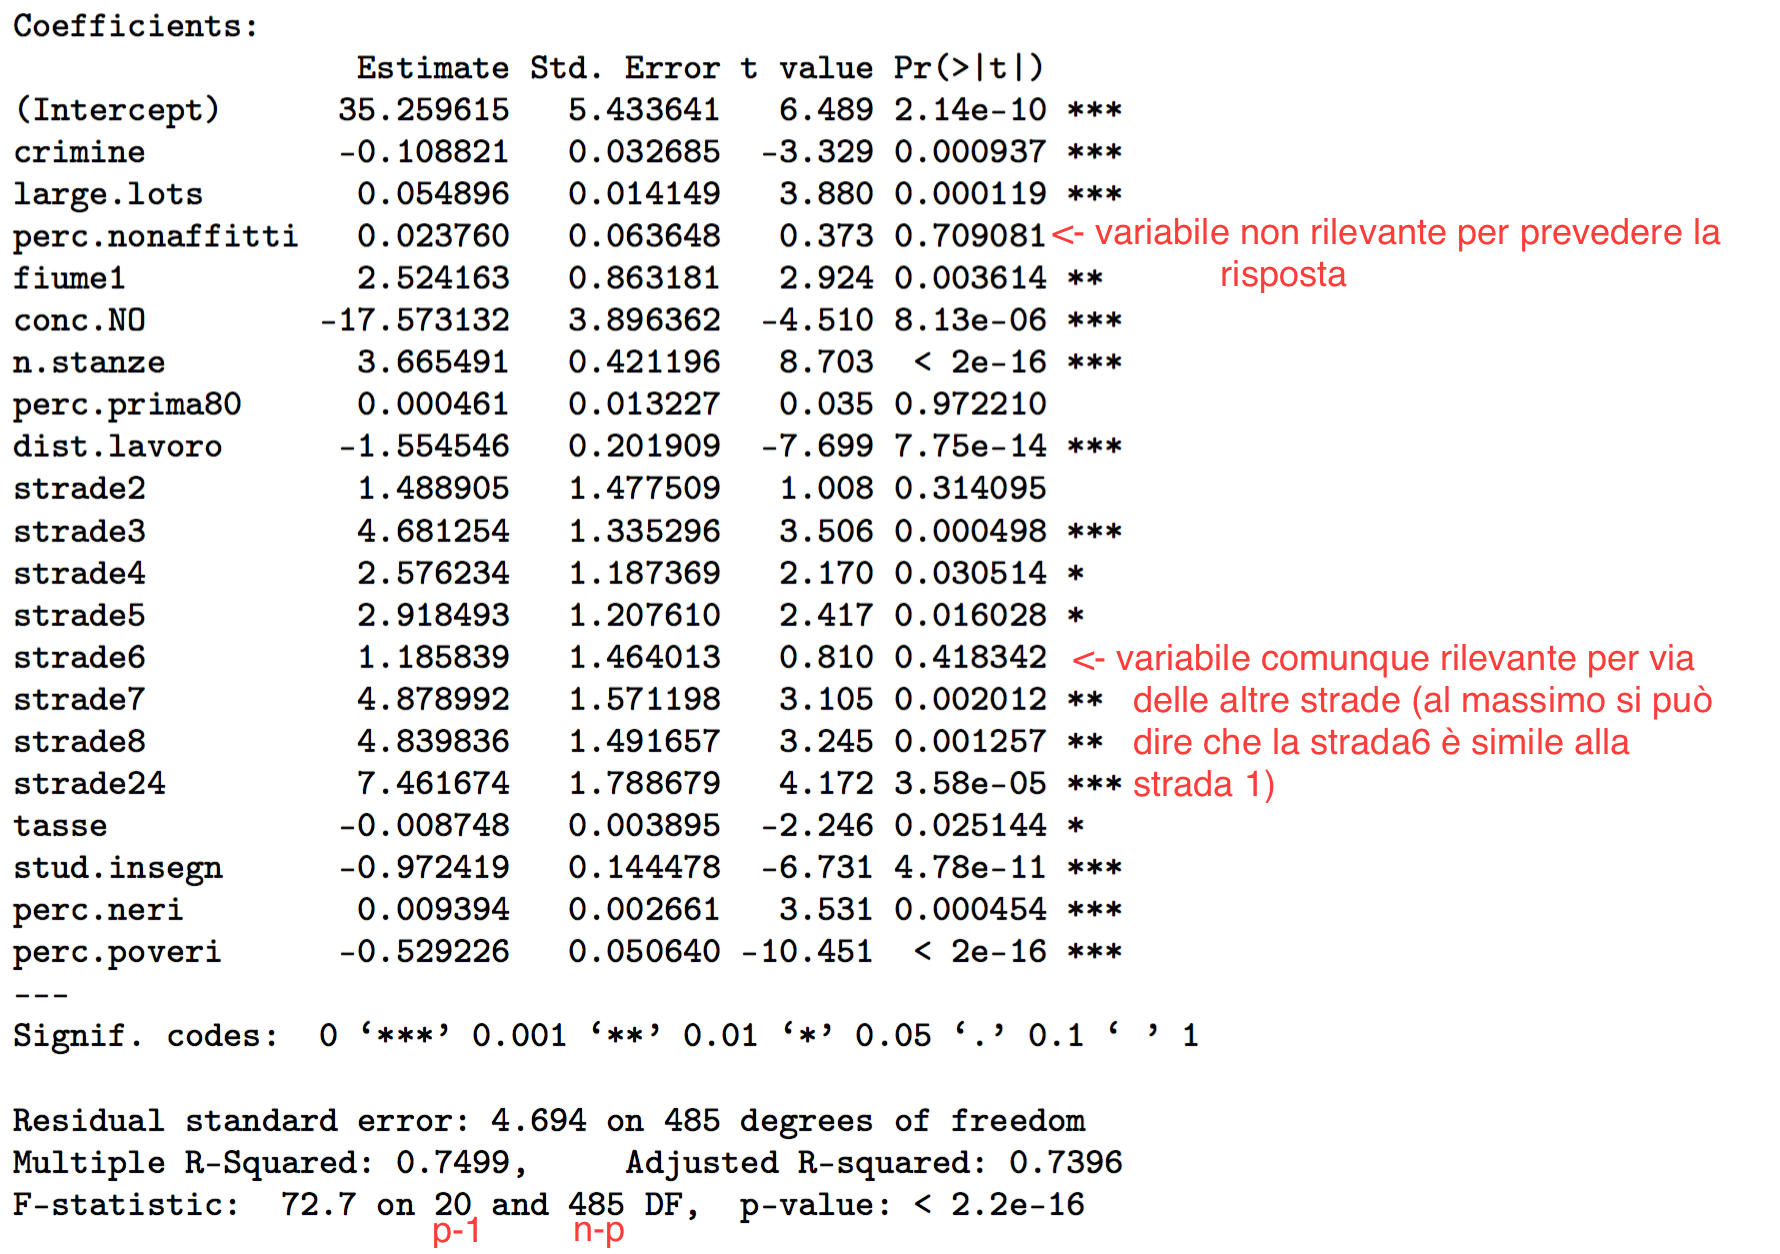
\includegraphics[width=.7\textwidth]{./notes/immagini/l10-fig1.png}
\end{figure}

\subparagraph{Dimostrazione}\label{dimostrazione-1}

Siano $ z_i $ e $ z_{i+p} $ dure caratteri di \textit{Z} a distanza \textit{p}. Siccome $ |\gamma|  \geq p$, i due caratteri possono essere appartenenti solamente o a \textit{X} o a \textit{Y} e mai ad entrambe le stringhe contemporaneamente. 
Pertanto dal momento che sia \textit{X} sia \textit{Y} hanno periodo \textit{p}, i due caratteri devono essere per forza uguali.

Da questo segue il lemma di periodicità che afferma che due periodi distinti \emph{p} e \emph{q} non possono coesistere troppo a lungo in
una stessa stringa senza che la stringa abbia anche periodo \emph{MCD(p,q)}.

\paragraph{Lemma - Lemma di periodicità}\label{lemma---lemma-di-periodicituxe0}

Sia \emph{X} una stringa di lunghezza \emph{n} con due periodi \emph{p}
e \emph{q} non entrambi nulli.

Se $n \geq p + q - MCD(p,q)$ allora la stringa \emph{X} ha anche periodo \emph{MCD(p,q)}.

\begin{figure}[htbp]
\centering
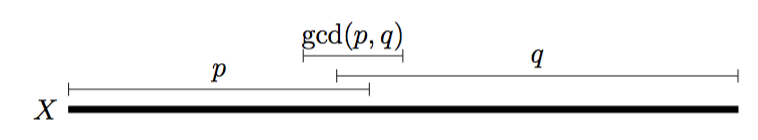
\includegraphics[width=.7\textwidth]{./notes/immagini/l10-fig2.png}
\caption{}
\end{figure}

\subparagraph{Dimostrazione}\label{dimostrazione-2}

Supponendo che $p \leq q$, la dimostrazione viene fatta per induzione su $p+q$.

$(p+q = 1)$ 

Se \emph{p=0} oppure \emph{p=q=0} allora \emph{MCD(p,q) = q} e dunque
\emph{X} ha periodo \emph{MCD(p,q)} perché ha periodo \emph{q}.

$(p+q > 1)$

Se \emph{p=0} o \emph{p=q} vale ancora il caso base.

Se $1 \leq p < q$, si ha che la stringa \emph{X} ha bordi $\alpha$ e $\beta$ di lunghezza \emph{n-p} e \emph{n-q}, questo per il primo lemma dimostrato.

\begin{figure}[htbp]
\centering
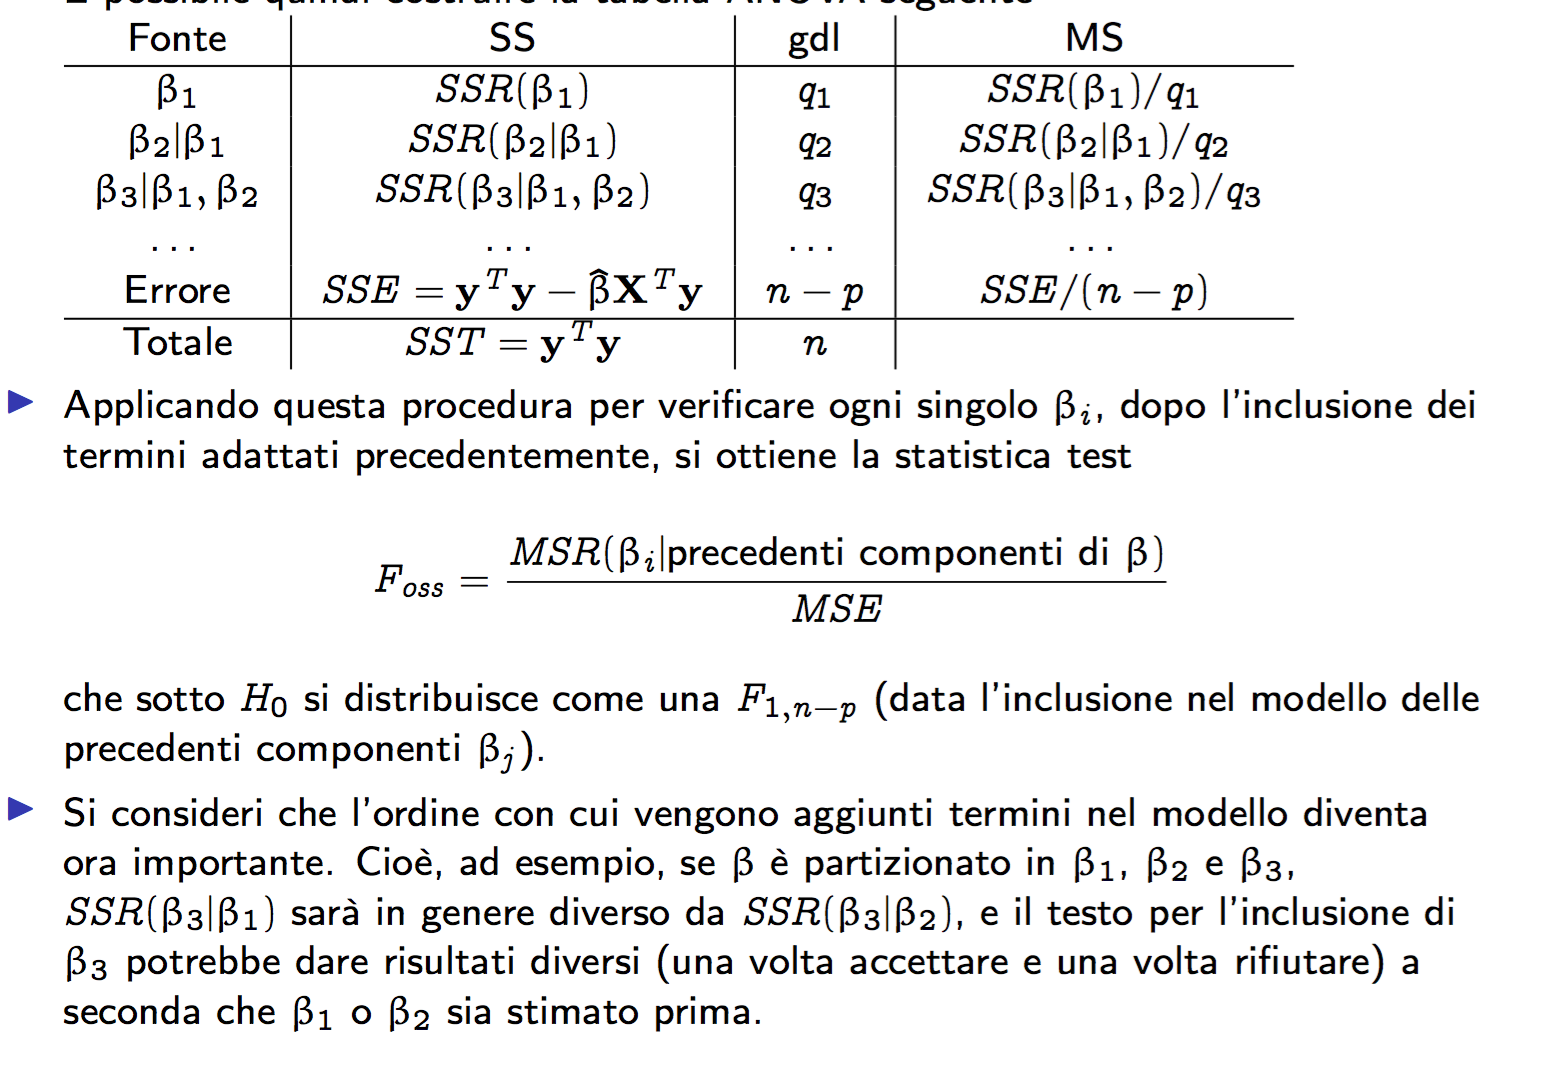
\includegraphics[width=.7\textwidth]{./notes/immagini/l10-fig3.png}
\caption{In verde la stringa $\alpha$ che si ripete con periodo
\emph{p}. In blu la stringa $\beta$ che si ripete con periodo
\emph{q}}
\end{figure}

La stringa $\beta$ essendo bordo di \emph{X} è anche bordo di $\alpha$ dal momento che $\alpha$ è un bordo di \emph{X}, pertanto $\alpha$ ha periodo $r = |\alpha| - |\beta| = q -p$.

Si ha che $p+r < p + q$, quindi è possibile applicare l'ipotesi induttiva, e che \emph{MCD(p,r) = MCD(p,q)}:

\begin{align*}
|\alpha| &\geq p+r-MCD(p,q)\\
 n - p &\geq q - MCD(p,q) 
\end{align*}

$ \alpha $ ha quindi come periodo sia \textit{r} (a causa di $ \beta $), sia \textit{p} (perché è una sottostringa di \textit{X}, la quale ha periodo \textit{p}) e per ipotesi induttiva ha anche periodo $MCD(p,r)$ che per come è definito \textit{r} è uguale a $MCD(p,q)$.

Considerando inoltre che:

\begin{align*}
	2|\alpha| &= (n-p) + (n-p) \\
					 &\geq q - MCD(p,q) + (n-p) \\
					 &\geq n
\end{align*}

perché $ p < q $ per ipotesi e $ MCD(p,q) \leq q - p $ per le proprietà del massimo comun divisore.

Questo implica che il prefisso $ \alpha $ di \textit{X} e il suffisso $ \alpha $ di \textit{X} coprono tutto \textit{X} e pertanto le due stringhe devono sovrapporsi\footnote{Non è possibile applicare il lemma della concatenazione perché non si sa di quanto queste stringhe si sovrappongono.} oppure $ X = \alpha\alpha $.

Presi quindi due caratteri $ x_i $ e $ x_j $ della stringa \textit{X}, tali che $ j - i = MCD(p,q) $ può succedere che i due caratteri appartengano alla stessa $ \alpha $ e quindi siano uguali, perché $ \alpha $ ha periodo $ r = MCD(p,q) $ oppure che $x_i \in \alpha_{(prefisso)} \text{ e } x_j \in \alpha_{(suffisso)} $.

\begin{figure}[htbp]
	\centering
	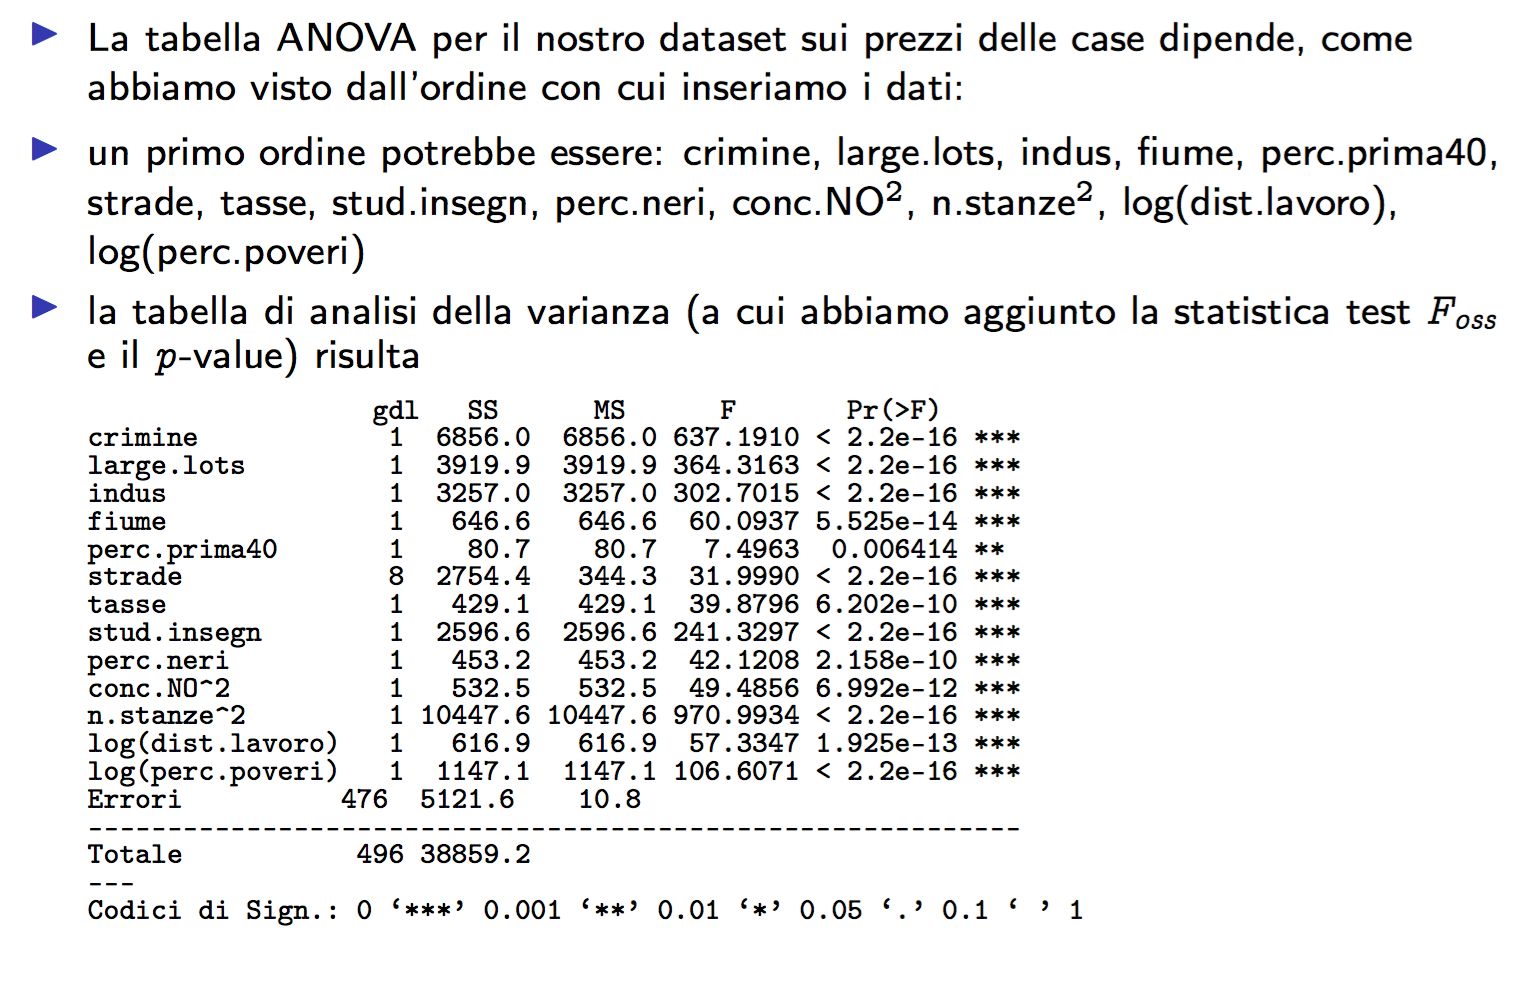
\includegraphics[width=.7\textwidth]{./notes/immagini/l10-fig4.png}
\end{figure}


In questo caso si ha che $ j > n - |\alpha| = p $ e quindi $ j - p \geq 1$. Si può quindi considerare il carattere $ x_{j-p} = x_j$ per via del periodo \textit{p} di $ X $ e che risulta appartenere a $ \alpha_{(prefisso)} $ perché $ p \geq MCD(p,q) $.

La distanza tra $ x_{j-p} \text{ e } x_i$ è $p - MCD(p,q)$, che per definizione è un multiplo di \textit{MCD(p,q)}, pertanto si ha che $ x_{j-p} \text{ e } x_i$ appartengono ad $ \alpha_{(prefisso)} $ che ha periodo \textit{MCD(p,q)}, pertanto $ x_{j-p} = x_i = x_j $ e di conseguenza \textit{X} ha periodo \textit{MCD(p,q)}.


\textbf{Sottostringa}: serie di caratteri vicini

\textbf{Sottosequenza}: serie di caratteri non necessariamente vicini.

\section{Pattern matching di base}\label{pattern-matching-di-base}

Effettua il pattern matching esatto, cercando la sotto stringa \emph{P}
dentro la stringa \emph{T}.

\begin{breakablealgorithm}
	\caption{Ingenuo: Pattern matching ingenuo}
	\begin{algorithmic}[1]
	\Function{Ingenuo}{$ (P,T) $}
	\State $  $ \Comment{\textit{T} ha lunghezza \textit{n} e \textit{P} ha lunghezza $ m \leq n $}
	\For{$ i = 1 \: \text{to} n-m+1 $}
		\State $ j \gets 1 $
		\While{$ j \leq m \:\text{and} \:P[j] = T[i+j-1] $}
	        \State $ j \gets j + 1 $
	    \EndWhile
	    \If{$ j > m $}
	        \State Segnala l'occorrenza del pattern
	    \EndIf
	\EndFor
	\EndFunction
\end{algorithmic}
\end{breakablealgorithm}

\subsection{Utilizzo della sentinella}\label{utilizzo-della-sentinella}

La prima modifica che si può fare all'algoritmo per migliorarne
l'efficienza è quello di ridurre il test del \texttt{while}, rimuovendo
il controllo sulla lunghezza del pattern, riducendo così le operazioni
da 3 a 2.

Questo viene fatto aggiungendo una sentinella alla fine del pattern,
ovvero viene aggiunto al pattern un carattere che non compare
nell'alfabeto della stringa.

Perché questo funzioni è necessario aggiungere un carattere diverso
dalla sentinella anche alla fine di \emph{T} per permettere il match del
pattern anche quando questo è un suffisso della stringa.

\begin{breakablealgorithm}
	\caption{Ingenuo: Pattern matching ingenuo}
	\begin{algorithmic}[1]
		\Function{Ingenuo-2}{$ (P,T) $}
        \State //\textit{T} ha lunghezza \textit{n} e \textit{P} ha lunghezza $ m \leq n $
        \State $ P[m+1] \gets \$ $
        \State $ T[n+1] \gets @$
        \For{$ i = 1 \: \text{to } n-m+1 $}
	        \State $ j \gets 1 $
	        \While{$ P[j] = T[i+j-1] $}
		        \State $ j \gets j + 1 $
	        \EndWhile
	        \If{$ j > m $}
		        \State Segnala l'occorrenza del pattern
	        \EndIf
        \EndFor
        \EndFunction
\end{algorithmic}
\end{breakablealgorithm}

Nel caso non sia possibile modificare il testo si può togliere il
\texttt{+1} del ciclo \texttt{for} e sostituirlo con un \texttt{if} che
verifica l'uguaglianza dell'ultimo carattere.

D'ora in avanti assumeremo la presenza dei due caratteri sentinella.

\subsection{Riduzione del numero di confronti}\label{riduzione-del-numero-di-confronti}

Se il pattern contiene delle sottostringhe uguali, è possibile ridurre
il numero di controlli.

Ad esempio nel caso sotto riportato, l'algoritmo \textsc{Ingenuo}
effettua 20 confronti.

\begin{figure}[htbp]
\centering
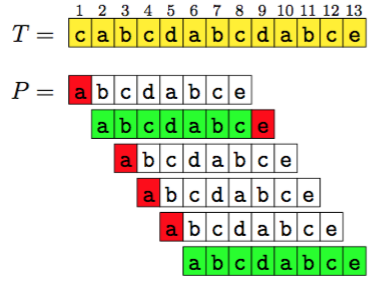
\includegraphics[width = .4\textwidth]{./notes/immagini/l11-fig1.png}
\end{figure}

Ovvero è possibile evitare il confronto tra l'inizio del pattern e il
terzo carattere del testo, perché si sa già che il terzo carattere del
testo è uguale al secondo carattere del pattern, il quale è diverso dal
primo carattere del pattern. Lo stesso ragionamento vale anche per i due
confronti successivi.

Ma si può fare di più, perché il pattern ha una sottostringa uguale al
suo prefisso, ovvero i caratteri 7-8-9 della del testo sono uguali ad
una sottostringa del pattern che coincide con il prefisso del pattern e
dal momento che questo è già questa uguaglianza è già stata verificata,
si possono ridurre ulteriormente i confronti.

\begin{figure}[htbp]
\centering
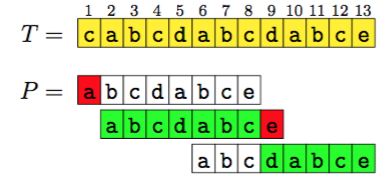
\includegraphics[width = .4\textwidth]{./notes/immagini/l11-fig2.png}
\end{figure}

Per poter applicare queste osservazioni ad un algoritmo è necessario
effettuare delle pre-elaborazioni delle stringhe.

\subsection{Pre-elaborazione fondamentale}\label{pre-elaborazione-fondamentale}

Data una stringa \emph{S} di lunghezza \emph{n}, la funzione
$\pi_i^S$ calcola la lunghezza del prefisso di \emph{S} più lungo
che occorre nella posizione \emph{i} di \emph{S}.

Quindi $\pi_i^S$ è il massimo \emph{h} tale che

$$
S[1,h] = S[i, i+h-1]
$$

Ad esempio:

\begin{figure}[htbp]
\centering
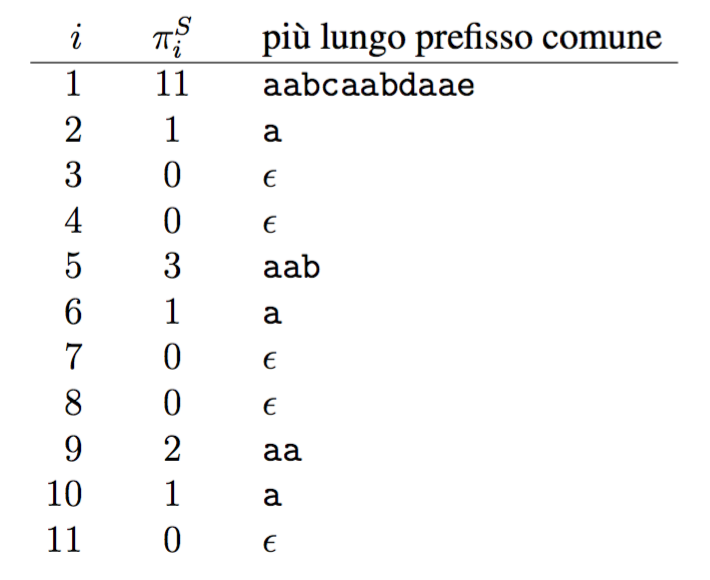
\includegraphics[width = .4\textwidth]{./notes/immagini/l11-fig3-bis.png}
\caption{$\pi_i$ per \textit{S=}\texttt{aabcaabdaae}.}
\end{figure}

Da notare che $Y = S[i, i+\pi_i -1]$ per definizione è un occorrenza in \textit{S} della stringa $S[1, \pi_i -1]$, pertanto si ha che \textit{Y} è un bordo della stringa $S[1, i +\pi_i -1]$. 
Per la relazione tra prefisso e bordo si ha quindi che $S[1, i +\pi_i -1]$ ha periodo $p = i -1$.

Si ha inoltre che la stringa $S[1, i +\pi_i -1]$ è il più lungo prefisso di \textit{S} con periodo $p= i-1$.

Questo perché se $i = 1$, si ha che il prefisso \textit{Y} coincide con \textit{S} e $p=0$, ottenendo periodo e bordo degeneri.

Se invece $ i \geq 2 $ si ha che, se $i + \pi_i -1 = n $, \textit{Y} è anche un suffisso di \textit{S}, pertanto non possono esserci altri prefissi con periodo $p = i -1$ più lunghi perché è la stringa \textit{S} è terminata.
Oppure se $i + \pi_i -1 \neq n $ vuol dire che il carattere $ S[\pi_i + 1] $ è diverso dal carattere $ S[i+\pi_i] $ per definizione di $ \pi_i $ e quindi non può esistere un prefisso $ S[1, \pi_i +1] $ con periodo $p = i -1$ perché $ S[\pi_i  + 1 + p] = S[\pi_i + i] $ che per ipotesi è diverso da $ S[\pi_i +1] $.

Le varie sottostringhe $ S[i, i + \pi_i -1 ] $ non sono necessariamente disgiunte ma possono sovrapporsi.

\subsubsection{Estremi massimi}

Fissato un $ i \geq 2 $, si ottengono varie stringhe $ S[j, j + \pi_j -1] $ con $ 2 \leq j \leq i $.

Tra tutte queste stringhe è possibile identificare la stringa che ha come valore dell' \textbf{estremo destro massimo}:

$$
r_i = \max \{ j + \pi_j -1 | \: 2 \leq j \leq i\}
$$

L'estremo sinistro associato viene indicato con 

$$
l_i = \arg\max\limits_{j} \{ j + \pi_j -1 | \: 2 \leq j \leq i\}
$$

Nel caso ci siano più sottostringhe con lo stesso estremo destro, viene scelto come estremo sinistro uno a caso tra quelli possibili.

La stringa $ S[l_i, r_i] $ risulta quindi essere la sottostringa di \textit{S} più lunga che è anche un prefisso e che inizia prima dell'indice \textit{i}.

\begin{figure}[htbp]
	\centering
	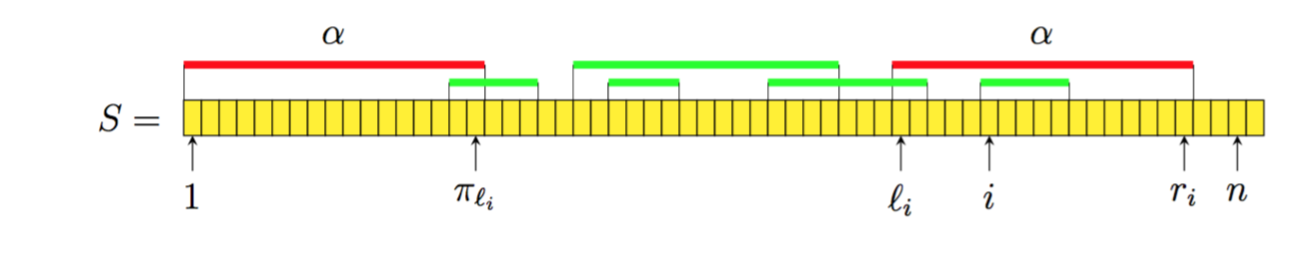
\includegraphics[width = .9\textwidth]{./notes/immagini/l11-fig4-bis.png}
	\caption{Alcune occorrenze di prefissi di \textit{S} che iniziano tra le posizioni \textit{2} e \textit{i}. L'occorrenza che termina più a destra è evidenziata in rosso.}
\end{figure}

Si ha quindi che $ S[1,r_i] $ è il più lungo prefisso di \textit{S} con periodo $ 1 \leq p < i $ e che la stringa $ S[l_i, r_i] $ è la sottostringa di \textit{S} che termina più a destra tra tutte quelle che sono uguali ad un prefisso di \textit{S}.

Ad esempio se 

$$
S = \text{\texttt{aabaabcadaabaabce}}
$$

il massimo destro con $ 2 \leq j \leq 15 $ è $ r_{15} = 10 + \pi_{10} -1 = 16$, perché $ \pi_{10} = 7$, e $ l_{15} = 10 $ che è la posizione in cui inizia la sottostringa \texttt{aabaabc}.

\subsection{Pre-elaborazione fondamentale in tempo lineare}\label{preambolazione-fondamentale-in-tempo-lineare}

Seguendo l'approccio di definizione il tempo richiesto è
$O(n^2)$, ma è possibile scendere a $O(n)$.

Supponiamo che \emph{S} termini con un carattere diverso da tutti gli
altri che compaiono nella stringa. Questo non è un problema perché si
può sempre aggiungere una sentinella.

L'algoritmo calcola $\pi_1 = n$ e poi calcola i valori $\pi_i, r_i, l_i$ per $i = 2,\ldots, n$, basandosi su un'array $ pref[1\ldots n] $ il quale conterrà i vari $ \pi_i $ e due variabili, \textit{r} e \textit{l}, le quali andranno a memorizzare gli estremi massimi tra gli indici precedente calcolati.

Come prima cosa viene effettuato il calcolo di $ \pi_2 $ confrontando da sinistra a destra i caratteri di $S[2,n]$, cosi facendo si ha che $ r = \pi_2 +1 $ e $l = 2$.

Assumendo induttivamente di aver calcolato $ \pi_j $ per ogni $ j = 2, \ldots, i-1$, si ha che $ r = r_{i-1} = \pi_{i-1} +1 $ e $ l = l_{i-1} $.

Durante il calcolo di $ \pi_i $ possono verificarsi 2 casi:

\begin{enumerate}
	\item $ i > r $: non si hanno informazioni riguardo ai caratteri che seguono \textit{i}, quindi viene effettuato il calcolo di $ \pi_i $ normalmente, andando ad effettuare i confronti da sinistra a destra tra $ S[i,n] $ e \textit{S}. Il valore di $ \pi_i $ è allora uguale alla lunghezza \textit{h} del massimo prefisso comune e $ r = i  + \pi_i +1 $ e $ l= i $.
	\item $ i \leq r$: il carattere \textit{S[i]} è contenuto nella sottostringa $ \alpha = S[l,r] $ la quale è anche prefisso di \textit{S}. Si ha quindi che il carattere \textit{S[i]} compare anche nella posizione $ i' = i - l +1 $ di \textit{S} e per lo stesso motivo la stringa $ \beta = S[i,r] $ compare anche in $ S[i', \pi_l] $.
	\begin{figure}[htbp]
		\centering
		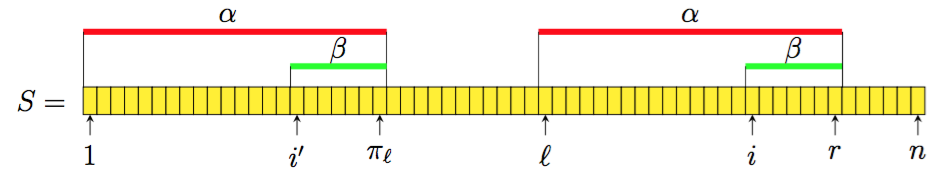
\includegraphics[width = .8\textwidth]{./notes/immagini/l11-fig3.png}
	\end{figure}
	In \textit{i'} occorrerà un prefisso $ \gamma $ di \textit{S} di lunghezza $ \pi_{i'} $, che può anche essere degenere.
	Questo prefisso occorrerà a partire dalle posizioni \textit{1} e \textit{i'} e potrà essere contenuto o contenere la sottostringa $ \beta $.
	Ne segue che \textit{S} e \textit{S[i,n]} hanno un prefisso in comune di lunghezza uguale al minimo tra $ \pi_{i'} $ e $ |\beta| = r - i +1 $.
	\begin{enumerate}
		\item $ \pi_{i'} < |\beta| $: il prefisso che inizia in \textit{i} ha la stessa lunghezza di quello che inizia in \textit{i'}, ed avendo già calcolato la lunghezza di quel prefisso si ha che $ \pi_i = \pi_{i'} $ senza effettuare alcun confronto.
		\begin{figure}[htbp]
			\centering
			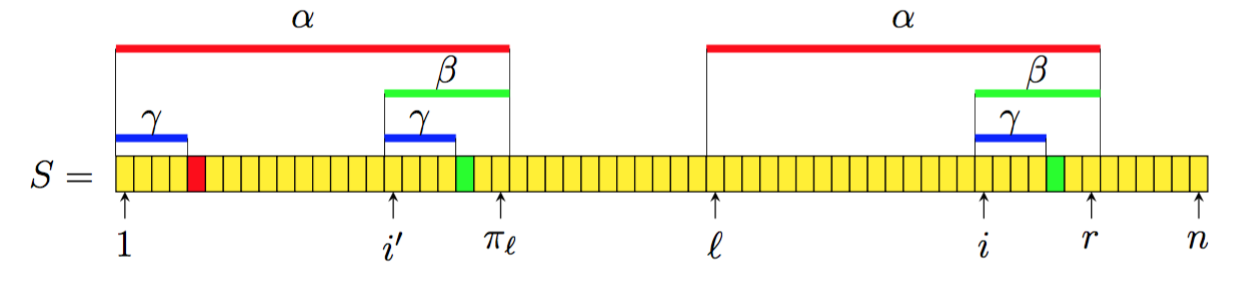
\includegraphics[width = .8\textwidth]{./notes/immagini/l11-fig5.png}
		\end{figure}
		\item $ \pi_{i'} \geq |\beta|$: l'intera sottostringa $ \beta = S[i,r] $ deve essere un prefisso di \textit{S} e quindi $\pi_i \geq |\beta| = r - i +1$. L'algoritmo calcola quindi la lunghezza \textit{h} del massimo prefisso comune tra \textit{S} e \textit{S[i,n]} a partire dai caratteri $ |\beta| + 1 $ e $ i + |\beta| $, fino a che non trova un mismatch. A questo punto vengono posti $ \pi_i =h,\: r= i + \pi_i -i \: \text{e} \: l = i $.
	\end{enumerate}
	
\end{enumerate}

\begin{breakablealgorithm}
	\caption{Prefisso: Preelaborazione del prefisso in tempo lineare}
	\begin{algorithmic}[1]
		\Function{Prefisso}{$ S $}
		    \State // S stringa di lunghezza n > 1 con sentinella alla fine
		    \State $ pref[1] \gets n $  \Comment{$ \pi_i, \pi_1 = n$}
		    \State $ h \gets 0 $
		    \While{$ S[1+h] = S[2+h] $}\Comment{Calcola $\pi_2$}
		        \State $ h = h +1 $
		    \EndWhile
		    \State $ pref[2] \gets h $
		    \State  $ l \gets 2 $
		    \State $ r \gets 2 + h - 1$
		    \For{$ i = 3 \: \text{to} \: n $}
			    \If{$ r < i $} \Comment{Caso 1}
			        \State $ h \gets 0$
		            \While{$ S[1+h] = S[i+h]$}
		                \State $ h \gets h + 1 $
		            \EndWhile
		            \State $ pref[i] \gets h$
		            \State $ l \gets i $
		            \State $ r \gets i + h -1 $
		        \Else \Comment{Caso 2}
				    \If{$pref[i-l+1] < r - i +1$} \Comment{Caso 2a}
		                \State $pref[i] \gets pref[i - l +1]$
		            \Else \Comment{Caso 2b}
		               \State $h \gets r - i +1$
		                \While{$S[1+h] = S[i +h]$}
		                    \State $ h \gets h +1 $
		                \EndWhile
		                \State $pref[i] \gets h$
		                \State $l \gets i$
		                \State $ r \gets i +h -i$
			         \EndIf
		          \EndIf
		    \EndFor
		    \State \Return $ pref $
		   \EndFunction
	\end{algorithmic}
\end{breakablealgorithm}

La correttezza dell'algoritmo deriva da quanto detto prima

\paragraph{Complessità}\label{complessituxe0}

Se non viene presa in considerazione la complessità dei cicli
\texttt{while} si ha che la complessità è data da \emph{O(n)}.

I cicli \texttt{while} terminano quando viene trovato un mismatch e al
massimo vengono trovati \emph{n-1} mismatch (1 dal \texttt{while}
esterno, $n-2$ dai \texttt{while} dentro il ciclo \texttt{for}).

Ad ogni confronto con successo, il carattere destro ($S[i+h]$)
viene spostato a destra di 1 e, una volta terminato il \texttt{while}, questo viene posto a $r = i + h - 1$, ovvero risulta essere il carattere alla posizione $S[r+1]$.

All'iterazione successiva il ciclo \texttt{while} inizia con carattere destro $S[i]$ se $i > r$\footnote{Viene quindi sposto a destra perché $ i \geq r+1 $} altrimenti inizia con $S[i + h]$ con $h = r - i + 1$. In entrambi i casi il carattere destro non si sposta mai a sinistra durante l'esecuzione dell'algoritmo. 
Pertanto vengono eseguiti al più $n-1$ confronti con successo. +
Si ottiene quindi una complessità per i \texttt{while} di $O(2n-2)$.

La complessità totale dell'algoritmo è data da $O(n) +\textit{ Complessità while }= O(n) + O(2n-2) = O(n)$.

\subsubsection{Matching esatto in tempo lineare}\label{matching-esatto-in-tempo-lineare}

Per effettuare il pattern matching in tempo $O(m+n)$ del pattern \emph{P} in \emph{T} è possibile utilizzare una versione leggermente modifica della funzione prefisso sulla stringa \emph{S = P\$T}, dove \$ è un simbolo che non è presente nelle due stringhe.

Questo viene fatto calcolando $ \pi_i^S $ per $ i = 2, \ldots n + m +1 $.
Siccome \$ non compare in nessuna delle due stringhe, si ha che $ \pi_i \leq m \: \forall \: i $ perché per ipotesi la sottostringa \textit{P\$} non può comparire all'interno di \textit{T}.
Inoltre, $ \forall \: i \geq m +1 : \pi_i = m $ si ha che $i - m - 1$ identifica l'inizio di un'occorrenza di \textit{P} in \textit{T}, perché $ \pi_i = m $ indica la presenza di prefisso di lunghezza \textit{m} a partire dalla posizione \textit{i}, ma la sottostringa prefissa di lunghezza \textit{m} coincide per costruzione con \textit{P}, quindi \textit{i} indica l'inizio di un'occorrenza del pattern \textit{P} nella stringa \textit{P\$T}.

Dal momento che il prefisso viene calcolato in tempo lineare rispetto la lunghezza della stringa, si ottiene una funzione di pattern matching con complessità lineare.

Altre caratteristiche di questo algoritmo sono:
\begin{itemize}
	\item il \textbf{consumo lineare di memoria} rispetto la lunghezza del pattern $ O(m) $, perché è possibile evitare di tenere in memoria tutti $ \pi_i $ con $ i >m $ perché tutti i valori \textit{i'} del caso 2 faranno sempre riferimento ai $ \pi_i \: \text{con}\: i \leq m $
	\item che non è necessario conoscere tutto l'alfabeto, basta avere la possibilità di confrontare i caratteri.
\end{itemize}

\subsubsection{Esercizio - Identificare una rotazione}

Date due stringhe \textit{X} ed \textit{Y} di uguale lunghezza \textit{n}, determinare in tempo lineare \textit{O(n)}, se \textit{Y} è una rotazione circolare di \textit{X}.
Ovvero se è possibile identificare due stringhe $ \alpha $ e $ \beta $ tali che $ X = \alpha\beta $ e $ Y = \beta\alpha $.

\paragraph{Soluzione}

Si concatenano le stringhe in modo da formare $ S = Y\$XX $, se eseguendo la preelaborazione trovo un prefisso di lunghezza \textit{n} a partire dal $n+1$ vuol dire che \textit{Y} compare tra le due \textit{X} e quindi le due stringhe sono la rotazione di una stessa stringa.

\subsubsection{Esercizio - Massima sottostringa comune}

Date due stringhe \textit{X} e \textit{Y} di lunghezza \textit{m} e \textit{n} calcolare, in tempo lineare, il più lungo suffisso di \textit{X} che è anche prefisso di \textit{Y}. 
Ovvero la sottostringa $ \gamma $ di lunghezza massima tale che $ X = \alpha\gamma \: \text{e} \: Y = \gamma\alpha$.

\paragraph{Soluzione}

L'idea è quella di concatenare due stringhe in modo da formare $ S= Y\$X $, dove \$ è un carattere che non compare in nessuna delle due stringhe, per poi effettuare la preelaborazione.

Se $ \pi_2^S = 0$ non c'è nessuna sottostringa uguale al prefisso di \textit{Y}, quindi $ \gamma = \epsilon $, altrimenti se  $ 0 < \pi_2^S = k \leq m$ si ha che c'è un'occorrenza all'interno di \textit{S} del prefisso di \textit{Y} lunga \textit{k}, ma non si ha alcuna garanzia che questa sia un suffisso per \textit{X}.

Se  $ \pi_{n+m+1-k}^S = k$ si ha che a partire dal carattere $ n+m+1-k $ c'è un match di una sottostringa di lunghezza \textit{k} che per costruzione è anche suffisso di \textit{X}, pertanto $ \gamma = Y[1,k] $, altrimenti la sottostringa precedentemente identifica si trova o all'interno di \textit{Y} o all'interno di \textit{X}, pertanto $ \gamma = \epsilon $.

\todo[inline]{Quasi corretto, bisogna andare a vedere i $ \pi_j $ per trovare il suffisso più lungo che è anche prefisso.}



\section{Lezione 13 - Support Vector Machine}\label{lezione-13---support-vector-machine}

Nelle precedenti puntate:

\begin{itemize}
\item
  Sappiamo che un iperpiano in uno spazio di dimensione \textit{m} ha VC
  dimension \textit{m+1}.
\item
  Si può aggiungere un vincolo di classificazione relativo al margine.
\item
  Per ottenere l'iperpiano con margine ottimo è necessario considerare
  l'ipotesi che minimizza la norma di \emph{w}.
\item
  Il tutto si fa con un polinomio di Lagrange e il suo duale.
\end{itemize}

\subsection{Dati non separabili linearmente}\label{dati-non-separabili-linearmente}

Tutto quello visto finora funziona se i dati sono linearmente
separabili.

Nel caso questi non lo siano è necessario permettere che alcuni vincoli possano essere violati e per fare ciò vengono introdotte delle nuove variabili $\xi_i \geq 0$, una per ogni vincolo (ovvero per ogni esempio del training set), tale che:

$$ y_i (\vec{w} \cdot \vec{x}_i + b) \geq 1 - \xi_i $$

Queste nuove variabili rappresentano la distanza dell'esempio \textit{i}-esimo dal margine.

\begin{figure}[htbp]
\centering
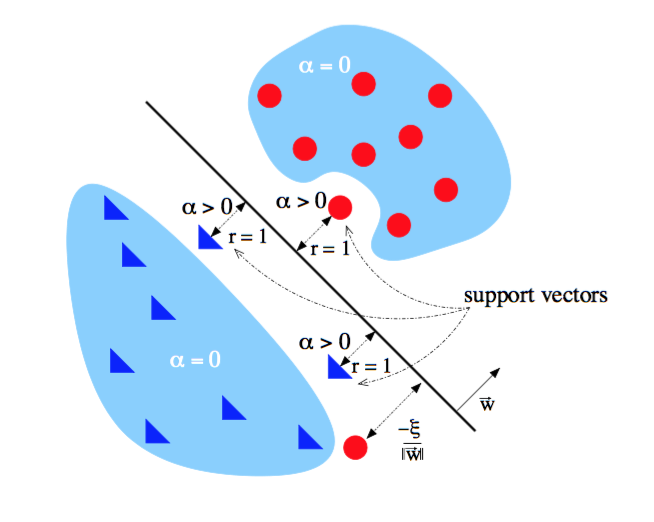
\includegraphics[width = 0.6\textwidth]{./notes/immagini/l13-non-linear.png}
\caption{SVM con dati non linearmente separabili.}
\end{figure}

L'idea è quindi quella di andare a sommare alla funzione costo la sommatoria di tutti i $\xi_i$ dei vari esempi presenti nel training set, moltiplicata per un coefficiente di penalizzazione \textit{C} che rappresenta un iper-parametro dell'algoritmo di apprendimento, da ottimizzare con le tecniche di model selection.

La nuova formula da minimizzare diventa:

$$ \frac{1}{2}||\vec{w}||^2 + C \sum\limits_{i=1}^n \xi_i $$

In pratica vengono penalizzati (aumentato il costo) gli esempi che non rispettano il margine.

La minimizzazione avviene considerano il problema duale, che risulta essere definito come:

$$max_\alpha \sum\limits_{i=1}^n \alpha_i - \frac{1}{2}\sum\limits_{i,j = 1}^n y_i y_j \alpha_i \alpha_j (\vec{x}_i \cdot \vec{x}_j)$$

$$ \text{s.t.: } \forall i \in \{1, \ldots, n\} : 0 \leq \alpha_i \leq C \text{ e } \sum\limits_{i=1}^n y_i \alpha_i = 0$$

Da notare che le $\xi_i$ sono variabili del problema primale e che quindi non compaiono nel problema duale.

Questa strategia per esempi non linearmente separabili non sempre
garantisce buone prestazioni perché un iper-piano può solo rappresentare
dicotomie dello spazio delle istanze.

Per questo motivo, quando gli esempi non sono linearmente separabili su
usa una strategia divisa in due passi:

\begin{enumerate}
\item
  Si mappano i dati di ingresso (input space) in uno spazio a dimensione
  molto superiore (feature space). Quindi a partire dalle feature degli
  elementi dell'input space vengono creati nuovi esempi nel feature
  space che utilizza combinazioni non lineari delle feature del primo
  spazio.
\item
  Si calcola poi l'iper-piano ottimo per il nuovo spazio usando la
  formulazione precedente (che prende il nome di variabili slack).
\end{enumerate}

Perché dovrei farlo?

\begin{enumerate}
\item
  Perché il \textbf{teorema sulla separabilità di Cover} afferma che un problema di classificazione complesso, formulato
  attraverso una trasformazione non lineare dei dati in uno spazio ad
  alta dimensionalità, ha maggiore probabilità di essere linearmente
  separabile che in uno spazio a bassa dimensionalità.
\item
  Perché l'iper-piano ottimo minimizza la VC-Dimension e quindi la
  capacità di generalizzazione migliora.
\end{enumerate}

Viene quindi utilizzata una trasformazione $\varphi(\cdot)$ non lineare, da applicare ai dati originari del problema $\{(\vec{x}_i, y_i)\}_1^n$ tale che:

$$ \forall i \: \vec{x}_i \in R^m, \varphi(\vec{x}_i) = \vec{Z}, \vec{Z} \in R^M, M \gg m $$

Il vettore ottenuto può essere rappresentato come $\vec{\varphi}(\vec{x}) = [ \varphi_1(\vec{x}), \ldots , \varphi_M(\vec{x}) ] $.

Con questa notazione è possibile andare a definire l'iper-piano nel nuovo spazio con:

$$ \sum\limits_{j=1}^M w_j \varphi_j(\vec{x}) + b = 0$$

che se si considera il termine noto $b = w_0$ e si aggiunge $\varphi_0(\vec{x}) = 1$, risulta essere

$$ \sum\limits_{j=0}^M w_j \varphi_j(\vec{x}) = \vec{w} \cdot \vec{\varphi}(\vec{x}) = 0$$

Andando a sostituire il $\vec{w}$ dell'equazione precedente con $ \vec{w} = \sum\limits_{k=1}^n j_k \alpha_k \vec{\varphi}(\vec{x}_k)$ si ottiene:

$$ \sum\limits_{k=1}^n j_k \alpha_k \varphi(\vec{x_k}) \cdot \varphi(\vec{x}) = 0 $$

Con il termine $\varphi(\vec{x}_k) \cdot \varphi(\vec{x})$ rappresenta il prodotto scalare tra un vettore del training set $\vec{x}_k$ e il vettore in input $\vec{x}$ calcolato nello spazio $R^M$.

\subsection{Funzioni Kernel}\label{funzioni-kernel}

Lo spazio di dimensione superiore serve solo per calcolare il prodotto scalare tra i due vettori, si può quindi definire una funzione $K(\cdot, \cdot)$ che prende il nome di kernel e che calcola il prodotto scalare dei due vettori senza passare esplicitamente nello spazio di dimensione superiore.

$$ K(\vec{x}_k, \vec{x}) = \varphi(\vec{x}_k) \cdot \varphi(\vec{x})$$

Assumendo di avere una di queste funzioni, l'iper-piano risulta essere:

$$\sum\limits_{k=1}^n  y_k \alpha_k K(\vec{x}_k, \vec{x}) = 0$$

Per il teorema di Mercer esistono delle funzioni di questo tipo, ma è necessario che soddisfino determinate condizioni.

Alcune di queste sono:

\begin{itemize}
\item \textbf{Polinomiale di grado \textit{p}}: $K(\vec{x},\vec{y}) = (\vec{x} \cdot \vec{y} +1) ^p$
\item \textbf{RBF}: $ K(\vec{x},\vec{y}) = exp(-\frac{1}{2\sigma^2}||\vec{x}-\vec{y}||^2)$
\end{itemize}

La formulazione duale del problema risulta quindi essere:

$$max_\alpha \sum\limits_{i=1}^n \alpha_i - \frac{1}{2}\sum\limits_{i,j = 1}^n y_i y_j \alpha_i \alpha_j K(\vec{x}_i ,\vec{x}_j)$$

$$ \text{s.t.: } \forall i \in \{1, \ldots, n\} : 0 \leq \alpha_i \leq C \text{ e } \sum\limits_{i=1}^n y_i \alpha_i = 0$$

Per fare la classificazione viene utilizzato il \textbf{segno} della funzione:

\begin{align*}
f(\vec{u})  &= \sum\limits_{i = 1}^n y_i  \alpha_i  K(\vec{x}_i,  \vec{u}) + b
\end{align*}

\subsection{Regressione}\label{regressione}

Quando si considera il problema di approssimazione di funzioni a valori
reali (regressione) si utilizza l'$\epsilon$-tubo: output che differiscono dai
valori di target per più di $\epsilon$ in valore assoluto vengono penalizzati
linearmente, altrimenti non vengono considerati errori. In pratica
aggiungo un intervallo di tolleranza al iper-piano che partiziona lo
spazio.

\begin{figure}[htbp]
\centering
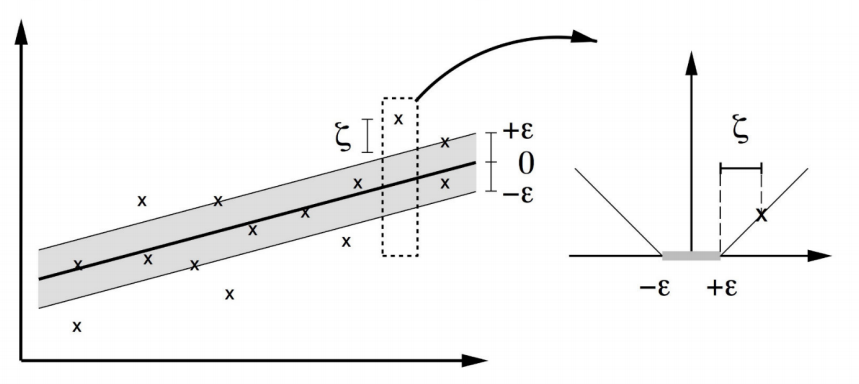
\includegraphics[width = 0.8\textwidth]{./notes/immagini/l13-primale-duale.png}
\caption{Regressione in forma primale (a sinistra) e duale (a destra)}
\end{figure}

\todo[inline]{Mancano formule (ultime due slide) http://www.math.unipd.it/\~{}aiolli/corsi/1516/aa/SVM.pdf}
% !TEX encoding = UTF-8
% !TEX program = pdflatex
% !TEX root = MEMOC.tex
% !TEX spellcheck = it-IT

% 15 Dicembre 2016

\todo[inline]{Da recuperare}
\section{Lezione 15 - Apprendimento Bayesiano}\label{lezione-15---apprendimento-bayesiano}

Si tratta di algoritmi di apprendimento basati sulla probabilità e sul
teorema di Bayes che effettuano la classificazione utilizzando l'ipotesi che
più probabilmente approssima la funzione target, scegliendola da un'insieme di funzioni $H$.

\subsection{Scelta delle ipotesi}\label{scelta-delle-ipotesi}

Tutto si basa sulla formula di Bayes.

$$
P(h | D) = \frac{P(D|h)P(h)}{P(D)}
$$

Dove:

\begin{itemize}
\item $P(h)$ è la probabilità a priori che l'ipotesi \textit{h} sia corretta e rispecchia la conoscenza a priori che si ha sul dominio;
\item $P(D)$ è la probabilità a priori che vengano osservati i dati \textit{D};
\item $P(h|D)$ è la probabilità che l'ipotesi \textit{h} sia corretta per i dati \textit{D};
\item $P(D|h)$ è la probabilità che i dati \textit{D} vengano classificati correttamente da \textit{h} \end{itemize}

L'obiettivo è quello di massimizzare \emph{P(h\textbar{}D)}, sapendo
\emph{P(D\textbar{}h)} che viene fornito dal supervisore e \emph{P(h)}
che viene appresa.

Nel massimizzare si può tralasciare il termine \emph{P(D)} dal momento
che è sempre costante.

$$
h_{MAP} = argmax_{h \in H} P(D|h)P(h)
$$

$H_{MAP}$ prende il nome di \textbf{ipotesi massima a posteriori}.

Si può inoltre assumere che tutte le ipotesi \emph{h} abbiano la stessa probabilità a priori, e nel mondo reale questa assunzione è tipicamente corretta, il
problema di massimizzazione diventa:

$$
h_{ML} = argmax_{h \in H} P(D|h)
$$

In questo caso si sceglie l'ipotesi di \textbf{maximum likelihood}

A pagina 158 del Mitchel c'è un esempio che mette in evidenza come le
probabilità a priori influenzino il risultato.

\subsection{Brute Force MAP Learning (interpretazione Find-S)}\label{brute-force-map-learning-interpretazione-find-s}

L'apprendimento dell'ipotesi massima avviene adattando l'algoritmo Find-S per l'apprendimento di concetti.

Si assumono fissate le istanze $x_1, \ldots, x_n$ e \textit{D} essere l'insieme dei valori desiderati $D = \{ c(x_1), \ldots, c(x_n)\}$.

Considerando inoltre tutte le ipotesi equiprobabili: $P(h) = \frac{1}{|H|}$, si ha che:

$$
P(D|h) = 
	\begin{cases}
		1,& \text{ se \textit{h} è consistente con \textit{D}} \\
		0,& \text{ altrimenti }
	\end{cases}
$$

L'algoritmo di apprendimento risulta quindi essere:

\begin{enumerate}
\item Per ogni potesi $h \in H$ calcola $P(h|D)$;
\item Scegli l'ipotesi che massimizza $P(h|D)$.
\end{enumerate}

Se i dati di apprendimento sono senza rumore e se la funzione target è contenuta nello spazio delle ipotesi \textit{H}, è possibile calcolare \emph{P(h\textbar{}D)} applicando la regola di Bayes, in particolare:

$$
P(h|D) = 
	\begin{cases}
		\frac{1}{|VS_{H,D}|},& \text{ se \textit{h} è consistente con \textit{D}} \\
		0,& \text{ altrimenti }
	\end{cases}
$$

Quindi se tutte le ipotesi \emph{h} sono equiprobabili, allora qualsiasi
ipotesi presente in \emph{H} va bene con probabilità $\frac{1}{VS_{H,D}}$, dove $VS_{H,D}$ è un sottoinsieme di \textit{H} consistente con \textit{D}.

Con questa definizione, tutte le ipotesi consistenti hanno probabilità $\frac{1}{VS_{H,D}}$ e tutte quelle non consistenti hanno probabilità \textit{0}, pertanto tutte le ipotesi consistenti possono essere delle $h_{MAP}$.

Segue anche che l'algoritmo Find-S ritorna sempre $h_{MAP}$ anche se non vengono utilizzate esplicitamente le probabilità.

Se vengono cambiate le probabilità in modo che la probabilità di
un'ipotesi più specifica sia più alta si ottiene che
\emph{P(h\textbar{}D) = P(h)}.

\subsection{Apprendimento di una funzione (ML)}\label{apprendimento-di-una-funzione-ml}

Si vuole apprendere una funzione $f$ a valori reali, utilizzando come esempi di apprendimento $(x_i, d_i)$ dove il valore target $d_i$ può contenere del rumore:

$$
d_i = f(x_i) + e_i
$$

dove $e_i$ è l'errore che segue una probabilità gaussiana con media 0 di
cui non si conosce la varianza.

Però si vuole valutare l'errore come se al posto di \emph{f} (che è sconosciuta) ci fosse \emph{h}

$$
e_i = d_i - h(x_i)
$$

La probabilità di $P(d_i | h)$, cioè che l'ipotesi \emph{h}
classifichi correttamente $d_i$ segue la distribuzione guassiana di
$e_i$.

Dalla definzione di ipotesi \textit{maximum likelihood} si ottiene che l'ipotesi $h_{ML}$ è anche quella che minimizza il quadrato degli errori:

\begin{align*}
h_{ML} &= argmax_{h \in H} P(D|h) \\
				&=  argmax_{h \in H} \prod\limits_{i=1}^m P(d_i|h) \\
				&= *\textit{gauassia di } e_i \textit{, logaritmi e altra math-magic*}\\
				&= arg min_{h \in H} \sum\limits_{i = 1}^m (d_i - h(x_i))^2
\end{align*}

Quindi per trovare l'ipotesi \textbf{maximum likelihood} è necessario
minimizzare l'errore quadratico, sotto l'ipotesi che la probabilità di
ogni ipotesi è uniforme e assumendo che i dati di apprendimento $d_i$ contengano del rumore che segue la distribuzione guassiana con media 0.

L'ipotesi \textit{MAP} coincide con l'ipotesi \textit{ML} solo se tutte le ipotesi hanno probabilità uniforme.

C'è anche da tenere in considerazione che questo approccio assume del rumore solamente nei dati $d_i$ e non dei vari $x_i$.

\subsection{Ipotesi MDL}

La scelta di questa ipotesi segue il principio del rasoio di Occam:``\textit{scegli la spiegazione più semplice per i dati osservati}'', ovvero sceglie l'ipotesi:

$$
h_{MDL} = argmin_{h \in H} L_{C_1}(h) + L_{C_2}(D|H)
$$

dove $L_C(x)$ è la lunghezza della descrizione di \textit{x} nella codifica \textit{C}.

Ad esempio, sfruttando la teoria dell'informazione è possibile utilizzare:

\begin{itemize}
\item $L_{C_1}(h) = - log_2(P(h))$
\item $L_{C_2}(D|h) = - log_2(P(D|h))$
\end{itemize}

Con questa codifica si ottiene che

\begin{align*}
h_{MDL} 	&= argmin_{h \in H} L_{C_1}(h) + L_{C_2}(D|H) \\
				&= argmin_{h \in H} - log_2(P(h)) - log_2(P(D|h)) \\
				&= argmax_{h \in H} P(D|h)P(h) \\
				&= h_{MAP}
\end{align*}

Ovvero che \textit{MDL} coincide con \textit{MAP}.

L'idea alla base di questo approccio è quella di effettuare un trade-off tra la complessità dell'ipotesi e il numero di errori commessi. L'ipotesi \textit{MDL} commette più errori sui dati di apprendimento a causa della sua brevità, ma ciò può essere visto come una limitazione dell'overfitting.

\subsection{Classificazione}\label{classificazione}

Finora abbiamo cercato l'ipotesi più probabile per i dati \emph{D}
($h_{MAP}$), ma dato un nuovo esempio, qual'è la classificazione più
probabile? Non sempre l'idea migliore è quella di calcolare $h_{MAP}(x)$.

Supponiamo di avere 3 ipotesi tali che: \emph{P($h_1$\textbar{}D)=0.4},\emph{P($h_2$\textbar{}D)=0.3},
\emph{P($h_3$\textbar{}D)=0.3} e che data una nuova istanza \emph{x} può si ottiene \emph{$h_1$(x) = (+)} e \emph{$h_2$(x) = $h_3$(x) = (-)}. 

In questo caso $h_{MAP}$, ovvero $h_1$, fornisce come classificazione $(+)$, anche se la classificazione più probabile è $(-)$.

Il \textbf{classificatore ottimo di Bayes} si basa su questo principio e classifica una nuova istanza $x$ con l'etichetta:

$$
v_x = argmax_{v_j \in V} \sum\limits_{h_i \in H} P(v_j | h_i)P(h_i | D)
$$

Dove:

\begin{enumerate}
\item $V$ è l'insieme di tutte le possibili classi
\item $
P(v_j | h_i) = 
	\begin{cases}
		1,& \text{ se } h_i(x) = v_j \\
		0,& \text{ altrimenti }
	\end{cases}
$
\end{enumerate}

Utilizzando lo stesso spazio delle ipotesi e la stessa conoscenza a priori, nessun altro classificatore riesce a superare il classificatore ottimo di Bayes.

Tuttavia, ad ogni classificazione è necessario calcolare la classificazione effettuata da ogni ipotesi $h_i$ e questo può essere computazionalmente oneroso al crescere del numero di ipotesi.

\subsection{Classificatore di Gibbs}\label{classificazione-di-gibbs}

Un'alternativa sub-ottima al classificatore di Bayes è data dall'algoritmo di Gibbs:

\begin{enumerate}
\item Sceglie un'ipotesi $h$ a caso, secondo $P(h|D)$,
\item utilizza l'ipotesi scelta per classificare l'istanza.
\end{enumerate}

Il classificatore così ottenuto è semplice da calcolare e funziona sorprendentemente bene dal momento che l'errore medio che compie è minore del doppio dell'errore effettuato dal classificatore ottimo:

$$
E[errore_{Gibbs}] \leq 2E[errore_{BayesOttimo}]
$$

Sempre assumendo probabilità a priori uniforme per tutte le ipotesi del version space.
\subsection{Verifica delle false occorrenze}\label{verifica-delle-false-occorrenze}

Il metodo di Rabin-Karp può trovare delle false occorrenze anche se la probabilità che queste compaiano è molto bassa .

L'algoritmo di Mathukrishnan serve per verificare se ci sono o meno delle false occorrenze in tempo \emph{O(n)}.

L'algoritmo prende in input la lista delle posizioni in cui c'è un'occorrenza vera o meno e identifica una falsa occorrenza utilizzando la distanza tra queste due posizioni.

Siano $ pos_{i-1} $ e $ pos_{i} $ due occorrenze consecutive segnalate dall'algoritmo di Karp e sia $ d = pos_{i} - pos_{i-1}$ la distanza tra queste.

Se $ d \leq m/2 $\footnote{Perché una stringa sia periodica, questa deve avere un periodo $ 0 \leq 2d \leq m $.} ed entrambe sono occorrenze effettive, il pattern \textit{P} ha un bordo di lunghezza $ m -d $ e quindi $ d  $ è un periodo sia del pattern, che della stringa $ T[pos_{i-1}, pos_{i} +m -1] $.

Inoltre, se \textit{P} avesse anche un periodo proprio $ p < d $ la porzione di testo $ T[pos_{i-1}, pos_{i} +m -1] $ dovrebbe avere anche essa il periodo $ p $ e quindi dovrebbe esserci un'occorrenza del pattern anche a partire da $ pos_{i-1} + p$, ma siccome non c'è questa occorrenza, la stringa non può avere periodo $ p $, quindi $ d $ è il più piccolo periodo proprio di $ P $.

L'algoritmo suddivide quindi le possibili occorrenze in \textbf{corse}, ovvero una sequenza di possibili occorrenze tali che $ pos_{i} - pos_{i-1} \leq m/2  $.

Se la corsa è composta da una sola posizione, l'algoritmo verifica direttamente se c'è un'occorrenza del pattern, confrontando il pattern con la stringa.

Se invece la cosa contiene più elementi $ pos_s, pos_{s+1}, \ldots, pos_{t} $, l'algoritmo verifica direttamente le prime due occorrenze $pos_{s}$ e $ pos_{s+1} $, se c'è una falsa occorrenza l'algoritmo termina, altrimenti la distanza $ d = pos_{s} - pos_{s+1} $ è il più piccolo periodo del pattern \textit{P} e quindi se per qualche $ i = s+2, \ldots, t  $ si ha che $ pos_i - pos_{i-1} \neq d $, l'algoritmo termina segnalando una falsa occorrenza.

Questo è corretto perché se $ pos_i - pos_{i-1} < d $, $ d $ non sarebbe il periodo minimo mentre se $ pos_i - pos_{i-1} > d $, c'è una falsa occorrenza perché dovrebbe esserci anche un'occorrenza intermedia.

Se l'algoritmo trova che tutte le distanze sono uguali a $ d $ deve soltanto controllare che la parte $ T[pos_s +m, pos_t + m -1] $ abbia effettivamente periodo $ d $ e questo viene fatto in tempo proporzionale alla lunghezza, confrontando tra loro i caratteri.


\begin{breakablealgorithm}
\caption{\textsc{MathukrishnanTest}: verifica della presenza di false occorrenze}
\begin{algorithmic}[1]
\Function{MathukrishnanTest}{$P,T,pos,k$}
	\If{$ k = 0 $}
		\State \Return false
	\EndIf
	\State $ j \gets 1 $
	\While{$ P[j] = T[pos[1] + j -1] $}
		\State $ j \gets j+1 $
	\EndWhile
	\If{$ j \leq m $} \Comment{è una falsa occorrenza}
		\State \Return True
	\EndIf
	\State $ i \gets 2 $
	\While{$ i \leq k $}
		\State $ j \gets 1 $
		\While{$ P[j] = T[pos[i] + j -1] $}
			\State $ j \gets j+1 $
		\EndWhile
		\If{$ j \leq m $} \Comment{è una falsa occorrenza}
			\State \Return True
		\EndIf
		\If{$ pos[i] - pos[i-1] \leq m/2$}
			\State $ s \gets i -1 $
			\State $ p \gets pos[s+1] - pos[s] $
			\While{$ i+1 \leq k \textbf{ and  } pos[i+1] - pos[i] = p$}
				\State $ i \gets i+1 $
			\EndWhile
			\If{$ i+1 \leq k \textbf{ and  } pos[i+1] - pos[i] \neq p$}
				\State \Return True
			\EndIf
		\EndIf
		\For{$ j \gets pos[s] +m +p \textbf{ to } pos[i] +m -1 $}\Comment{tutte le posizioni della corsa sono a distanza corretta, controllo se la porzione di testo ha periodo $p $}
			\If{$ T[j] \neq T[j-p] $}
				\State \Return True
			\EndIf
		\EndFor
	\EndWhile
\EndFunction
\end{algorithmic}
\end{breakablealgorithm}

\subsubsection{Complessità}\label{complessituxe0}

Per ogni corsa si hanno al massimo $pos_t - pos_s - d$ caratteri da verificare, se il risultato è negativo viene segnalata una falsa occorrenza e l'algoritmo termina, altrimenti passa alla corsa successiva.

Durante la verifica di una corsa, ogni carattere del testo viene confrontato al massimo 2 volte con i caratteri del pattern più 1 volta con il carattere successivo del testo.

Dal momento che le corse distinte non si sovrappongono, si ha che vengono fatti al massimo \emph{O(3n)} confronti, che portano ad una complessità di \emph{O(n)}.

\section{Alberi dei suffissi}\label{alberi-dei-suffissi}

L'albero dei suffissi permette di evidenziare maggiormente la struttura interna di una stringa, permettendo così di risolvere in tempo lineare il pattern matching esatto, così come altri problemi di pattern matching più complesso.

Con il pattern matching esatto è possibile effettuare una pre-elaborazione del testo in \emph{O(n)} dopo la quale è possibile verificare in tempo \emph{O(m)} la presenza del pattern, rendendo questi algoritmi adatti ai problemi che hanno un testo fisso che deve essere matchato con più pattern distinti.

L'\textbf{albero dei suffissi} per una stringa \emph{S} di lunghezza \emph{n} è costituito da:

\begin{itemize}
\item  \emph{n} foglie numerate da 1 ad \emph{n}.
\item  Ogni nodo interno, eventualmente esclusa la radice, ha almeno due figli.
\item  Ogni arco è etichettato con una sottostringa di \emph{S}.
\item  Due archi uscenti dallo stesso nodo non possono avere etichette che iniziano con lo stesso carattere.
\item  La concatenazione delle etichette lungo il cammino dalla radice alla foglia etichettata \emph{i} è il suffisso $S[i,n]$ di lunghezza $ n-i+1 $
\end{itemize}

\begin{figure}[htbp]
\centering
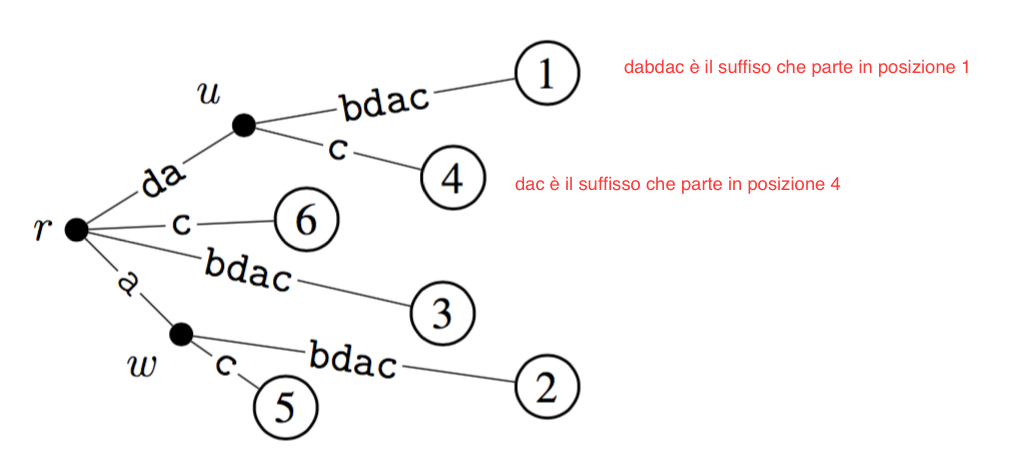
\includegraphics[width=.7\textwidth]{./notes/immagini/l19-fig1.png}
\caption{Albero dei suffissi della stringa $ S = dabdac $}
\end{figure}

Da notare che non sempre è possibile costruire l'albero dei suffusi, perché se un suffisso è anche prefisso di un altro suffisso, il cammino relativo a quel suffisso termina in un nodo interno dell'albero, violandone la definizione. 
Per evitare questo problema è necessario aggiungere un carattere sentinella alla fine della stringa. Assumeremo che questa ci sia sempre.

Nell'esempio \emph{S=dabdac} è \emph{c} che fa da sentinella, se non ci fosse non sarebbe possibile costruire l'albero.

L'\textbf{etichetta di un cammino} è la concatenazione delle etichette degli archi del cammino, mentre l'etichetta di un nodo \emph{u} è data dall'etichetta del cammino dalla radice al nodo.

Se l'etichetta di un arco $ (u,v) $ tra due nodi interni ha lunghezza \textit{k} maggiore di 1, l'arco è in realtà diviso in \textit{k} parti, una per ogni carattere dell'etichetta, mediante $ k-1 $ \textbf{nodi impliciti} le cui etichette sono la concatenazione dell'etichetta di \textit{u} con i caratteri dell'etichetta dell'arco $ (u,v) $ che precedono il nodo stesso.

\subsection{Matching esatto con l'albero dei suffissi}\label{matching-esatto-con-lalbero-dei-suffissi}

\begin{enumerate}
	\item Costruisci l'albero dei suffissi \textit{A} per il testo \textit{T}.
	\item Confronta i caratteri del pattern \textit{P} con i caratteri dell'unico cammino in \textit{A} individuato da essi. Questo cammino è unico perché tutti gli archi uscenti di un nodo sono associati a caratteri distinti. Seguendo questo cammino si possono verificare due casi:
	\begin{enumerate}
		\item Si esauriscono i caratteri del pattern e si passa al passo successivo
		\item Ci sono ancora dei caratteri del pattern ma non è possibile proseguire il cammino, in questo caso non ci sono occorrenze del pattern nel testo e l'algoritmo può terminare.
	\end{enumerate}
	\item Se si arriva alla fine del pattern, allora questo è uguale all'etichetta del nodo \textit{u} a cui si è arrivati, indipendentemente dal fatto che \textit{u} sia un nodo implicito o meno. Il pattern \textit{P} è quindi prefisso di tutti i suffissi associati alle foglie del sotto-albero radicato in \textit{u}. Le posizioni d'inizio di questi suffissi sono quindi tutte e sole le posizioni in cui \textit{P} occorre in \textit{T} e dal momento che queste posizioni sono memorizzate nelle foglie del sotto-albero, è sufficiente esplorarlo fino alle foglie per risalire alle posizioni di occorrenza del pattern.
\end{enumerate}

\subsubsection{Complessità del matching esatto}\label{complessituxe0-del-matching-esatto}

C'è una complessità \emph{O(n)} per la costruzione dell'albero (che per il momento non è stata vista).

Durante il secondo passo, per ogni carattere del pattern viene fatto
\begin{itemize}
	\item Un confronto se l'algoritmo sta analizzando un nodo implicito (c'è un solo arco uscente)
	\item Al più tanti confronti quanti sono i caratteri dell'alfabeto se è un nodo esplicito (al massimo ci sono tanti archi uscenti quanti sono i caratteri dell'alfabeto).
\end{itemize}

In ogni caso il numero di confronti è minore o uguale di una costante e quindi il passo 2 ha complessità $ O(m) $.

Il terzo passo richiede tempo proporzionale al numero di nodi del sotto-albero radicato in \textit{u}.
Se nel testo ci sono \textit{k} occorrenze del pattern, questo sotto-albero ha esattamente \textit{k} foglie e siccome ogni nodo interno ha almeno due archi uscenti, il numero di nodi interni è $ \leq k-1 $, quindi il terzo passo richiede $ O(k) $.

Siccome $ k \leq n $, il tempo totale richiesto è $ O(n+m) $, come per gli altri algoritmi, con la differenza che il carico di lavoro è sbilanciato verso la preelaborazione e non verso la ricerca (risulta più conveniente cercare più pattern nello stesso testo).

\subsection{L'algoritmo naive per la costruzione dell'albero} \label{lalgoritmo-naive-per-la-costruzione-dellalbero}

L'albero dei suffissi per la stringa $S[1,n]$ viene costruito a partire dal suffisso più lungo della stringa \textit{S}, ovvero tutta la stringa, per poi aggiungere gli altri suffissi $S[i,n]$ con $i = 2, \ldots, n+1$. 

Con $A_i$ viene indicato l'albero intermedio che contiene tutti i suffissi che iniziano nelle posizioni da 1 a \emph{i}.

L'albero $A_1$ contiene solamente un unico arco etichettato con $S[1,n]\$$ che congiunge la radice e il nodo \emph{1}.

Ogni albero $A_{i+1}$ viene costruito nel seguente modo:

\begin{enumerate}
	\item Partendo dalla radice di $ A_i $ viene cercato il più lungo cammino che raggiunge un nodo la cui etichetta è prefisso del suffisso $ S[i+1,n]\$ $ da aggiungere.
	
	Il cammino che si ottiene è unico in quanto ogni nodo implicito ha un solo arco uscente e tutti gli archi uscenti da uno stesso nodo esplicito sono associati a caratteri diversi.
	Inoltre, la ricerca deve terminare prima della fine del suffisso $ S[i+1,n]\$ $ perché la sentinella assicura che il suffisso non sia prefisso di nessuno dei prefissi più lunghi inseriti precedentemente nell'albero.
	
	\item Se il nodo in cui termina la ricerca è implicito, questo viene sostituito da un nodo esplicito, spezzando l'arco che lo contiene in due archi e l'etichetta in due etichette.
	
	\item A questo punto il nodo \textit{u} sul quale è terminata la ricerca è un nodo esplicito con etichetta $ S[i+1,j] $ tale che nell'albero non ci sia un nodo con etichetta $ S[i+1,j+1] $ e quindi tutti gli archi uscenti hanno etichette che iniziano con un carattere diverso da $ S[j+1] $.
	
	Viene quindi aggiunto un nuovo arco uscente da \textit{u} a $ i+1 $ con etichetta $ S[j+1,n]\$ $ che congiunge \textit{u} con la foglia numerata $ i+1 $.
	
	A questo punto l'albero ottenuto contiene un unico cammino dalla radice alla foglia $ i+1 $ la cui etichetta è il suffisso $ S[i+1,n]\$ $, ovvero l'albero ottenuto è $ A_{i+1} $
\end{enumerate}

\subsubsection{Complessità dell'algoritmo}\label{complessituxe0-dellalgoritmo}

Quando devo aggiungere un suffisso vengono passati al più tutti caratteri del suffisso e non appena viene trovato un carattere diverso, vengono aggiunti tanti nodi quanti sono i caratteri del suffisso restanti, ottenendo così una complessità $ O(n) $.
Dal momento che una stringa di lunghezza \textit{n} ha \textit{n} suffissi distinti, la complessità totale dell'algoritmo è $ O(n^2) $, dove $ n^2 $ è moltiplicato per una costante pari alla cardinalità dell'alfabeto.

\subsection{Algoritmo di Ukkonen}\label{algoritmo-di-ukkonen}

Questo algoritmo costruisce l'albero dei suffissi un carattere alla volta, partendo dall'inizio della stringa.

Così facendo viene persa la condizione che un suffisso non possa essere un prefisso dell'albero, per questo si dice che l'algoritmo crea una successione di \textbf{alberi dei suffissi impliciti}.

Un albero dei suffissi implicito è un albero simile a quello normale, con la differenza che viene rimossa la condizione che il cammino relativo ad ogni suffisso della stringa \textit{S} termini in una foglia e viene preso in considerazione anche il suffisso nullo.

\begin{figure}[htbp]
	\centering
	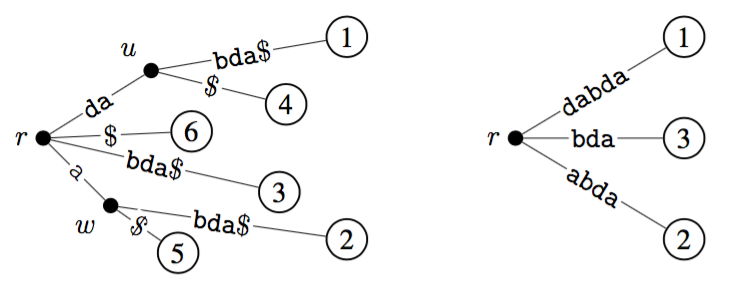
\includegraphics[width=.7\textwidth]{./notes/immagini/l19-fig2.png}
	\caption{Albero dei suffissi normale e implicito per la stringa $ S = dabda $.}
\end{figure}

L'algoritmo di Ukkonen costruisce un albero dei suffissi implicito $ I_i $ per ogni prefisso $ S[1,i] $ della stringa $ S\$ $ di lunghezza $ n+1 $ e incrementando \textit{i} finché non arriva a costruire $ I_{n+1} $. Siccome $ S[1,n+1] = S\$ $, l'albero dei suffissi implicito $ I_{n+1} $ coincide con l'albero dei suffissi \textit{A}, perché nessun suffisso della strina $ S\$ $ è prefisso di un altro suffisso.

\begin{breakablealgorithm}
	\caption{Ukkonen: Descrizione generale dell'algoritmo }
	\begin{algorithmic}[1]
		\Function{Ukkonen}{$S$}
			\State $ S \gets S\$ $ \Comment{Aggiunge la sentinella a $ S $}
			\State ``Costruisci $ I_0 $ ''
			\For{$ i = 0 \textbf{ to } n $}
				\For{$ j = 1 \textbf{ to } i+1 $}
					\State ``Cerca la fine del cammino relativo al suffisso $ S[j,i] $ in $ I_i $''
					\State ``Se necessario estendi il cammino con il carattere $S[i+1] $ in modo che il suffisso $ S[j,i] $ diventi un suffisso di $ S[1,i+1] $''
				\EndFor
			\EndFor
		\EndFunction
	\end{algorithmic}
\end{breakablealgorithm}

La costruzione di $ I_0 $ è banale in quanto contiene solo la radice e nessun arco uscente, perché la stringa $ S[1,0] $ ha come suffisso solamente $ \epsilon $.

Per costruire $ I_{i+1} $ è necessario modificare tutti i suffissi $ S[j,i] $ di $ S[1,i] $ nei suffissi $ S[j,i+1] $ di $ S[1,i+1] $.
Durante questa modifica possono verificarsi 3 casi:

\begin{enumerate}
	\item Il cammino etichettato $ S[j,i] $ termina in una foglia numerata $ j $. In questo caso il nuovo carattere $ S[i+1] $ viene aggiunto all'etichetta dell'ultimo arco del cammino (viene messo un nuovo nodo implicito).
	\item Il cammino etichettato $ S[j,i] $ termina in nodo interno \textit{u}, ma nessun cammino che parte da \textit{u} inizia con $ S[i+1] $. In questo caso viene creata una foglia etichettata $ j $ connessa al nodo \textit{u} con un arco etichettato $ S[i+1] $. Se \textit{u} è un nodo implicito, viene sostituito con un nodo esplicito, spezzando l'arco esistente.
	\item Il cammino etichettato $ S[j,i] $ termina in nodo interno \textit{u} e almeno un cammino che parte da \textit{u} è etichettato con $ S[i+1] $. In questo caso il suffisso $ S[j,i+1] $ è già presente nell'albero e non occorre fare niente.
\end{enumerate}

Dopo aver esteso tutti i suffissi di $ S[1,i] $ l'albero contiene tutti i suffissi di $ S[1,i+1] $, compreso il suffisso nullo che è sempre rappresentato.

\begin{figure}[htbp]
	\centering
	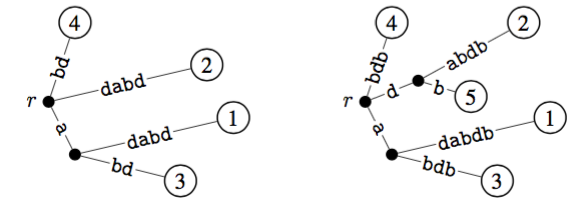
\includegraphics[width=.7\textwidth]{./notes/immagini/l19-fig3.png}
	\caption{Estensione dell'albero dei suffissi implicito per la stringa $ adabd $ quando si aggiunge alla stringa il carattere $ b $. I primi 4 suffissi vengono estesi con il caso 1, il quinto viene esteso con il caso 2 e il suffisso nullo viene esteso per il caso 3.}
\end{figure}

Tuttavia con questa implementazione si riesce a calcolare in $ O(i^2) $ l'albero $ I_{i+1} $ a partire da $ I_i $, portando ad una complessità totale di $ O(n^3) $ che è peggiore di quella dell'algoritmo naive.



\subsection{Miglioramento dell'efficienza con i Suffix Link}

Un primo miglioramento lo si ottiene utilizzando i \textbf{suffix link}, ovvero un collegamento tra due nodi espliciti dell'albero \textit{u} e $ s(u) $ tali che l'etichetta di $ u $ sia $ x\alpha $ e l'etichetta di $ s(u) $ sia $ \alpha $, in altre parole c'è un suffix link se l'etichetta di $ u $ è uguale all'etichetta di $ s(u) $ preceduta da un carattere qualsiasi (Fig \ref{asdasdasd2}).

\begin{figure}[htbp]
	\centering
	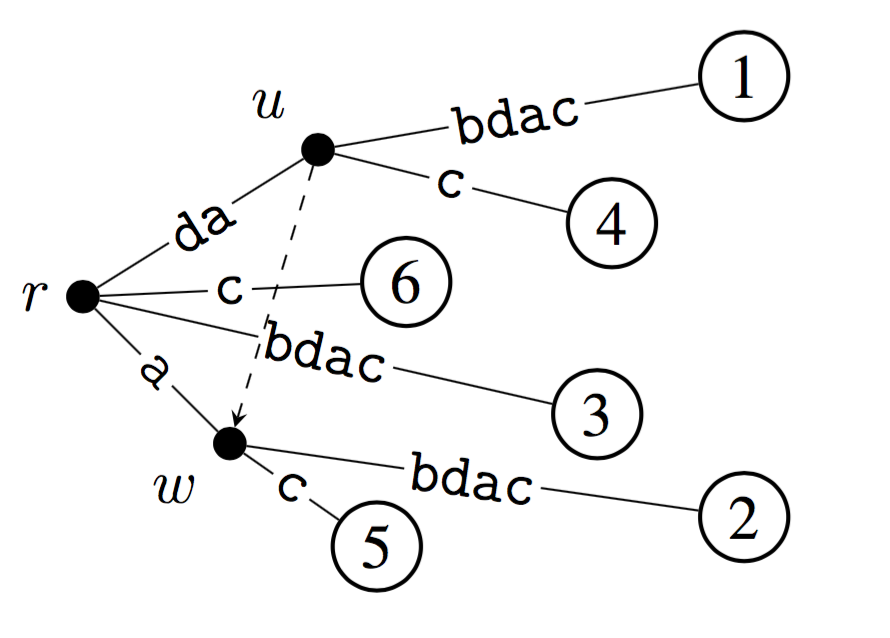
\includegraphics[width=.4\textwidth]{./notes/immagini/l22-fig1.png}
	\caption{In questo caso $\alpha=a$ e $x=d$}\label{asdasdasd2}
\end{figure}

Così facendo durante la costruzione dell'albero, quando viene esteso il cammino ad una foglia, posso tornare indietro fino a che non trovo un nodo esplicito con un suffix link e posso riprendere la costruzione dell'albero a partire dal nodo collegato.

Per ogni albero implicito $ I_i $, ogni nodo esplicito ha un suffix link uscente (\textbf{Lemma 5.4}), perché se durante la fase \textit{i}-esima per estendere il suffisso $ S[j,i] $, viene creato un nuovo nodo non foglia con etichetta $ x\alpha $ ($x\alpha$ prefisso di $ S[j,i] $) allora:

\begin{itemize}
	\item o nell'albero corrente esiste già un nodo interno esplicito con etichetta $\alpha$. Ad esempio perché la stringa $\alpha$ è un prefisso del suffisso $S[j+1, i-1]$ precedentemente inserito nell'albero.
	\item oppure tale nodo verrà creato immediatamente dopo con l'estensione del suffisso successivo $ S[j+1,i] $.
	
	Questo perché un nuovo nodo interno esplicito \textit{v} con etichetta $ S[j,i] = x\alpha $ viene creato soltanto se il suffisso $ S[j,i] $ viene esteso con il caso 2, quando nell'albero corrente il cammino $ S[j,i] $ termina in un nodo interno implicito e tale cammino continua con un carattere \textit{c} diverso da $S[i+1]$.
	Quindi nell'albero corrente c'è anche il cammino di etichetta $S[j+1,i] = \alpha$ che ha una continuazione che inizia con il carattere \textit{c}.
\end{itemize}

Dunque il nodo $ w $ con etichetta $ S[j+1, i]  = \alpha$ è un nodo interno che può essere esplicito o implicito. Se è esplicito $w = s(v)$ altrimenti, il cammino di etichetta $ S[j+1, i] = \alpha $ che termina nel nodo \textit{w} può continuare solo con \textit{c} e quindi nel passo successivo l'estensione del suffisso $ S[j+1,i] $ sostituisce il nodo implicito con un nodo esplicito per cui $s(v) = w$.

Inoltre (\textbf{Corollario 5.5}), nell'algoritmo di Ukkonen, ogni nodo interno esplicito creato durante l'estensione di un suffisso ha sicuramente un suffix link da esso uscente dopo che sia stato esteso anche un il suffisso successivo.

Questo si dimostra per induzione. Per $ I_0 $ la cosa è banalmente vera perché è presente solo un nodo interno esplicito e la radice non viene creata estendendo un suffisso.

Supponendo quindi che al termine della fase $(i-1)$-esima ci siano tutti i suffix link, per il lemma precedente, se viene creato un nuovo nodo \textit{v} estendendo $ S[j,i] $, il nodo $ s(v) $ viene trovato o creato durante l'estensione del suffisso successivo $ S[j+1,i] $. Siccome l'estensione dell'ultimo suffisso $ S[i+1,i] $ non aggiunge nodi interni, alla fine della fase $ i $-esima, tutti i nodi interni espliciti hanno il loro suffix link.

In altre parole, in ogni albero dei suffissi impliciti $ I_i $, se un nodo interno esplicito ha etichetta di cammino $ x\alpha $ esiste anche un nodo interno esplicito di etichetta $\alpha$.

\subsubsection{Costruzione dell'albero utilizzando i suffix link}

Nella fase di costruzione dell'albero $ I_{i+1} $ (fase $ i $-esima), l'algoritmo di Ukkonen cerca i nodi in cui terminano i suffissi $ S[j,i] $ per estenderli con il carattere $ S[i+1] $ (Nella fase $i$-esima viene esteso l'albero implicito $I_i$ per ottenere l'albero implicito $I_{i+1}$).

Il cammino relativo al suffisso $ S[1,i] $ sarà sempre presente e terminerà ogni volta in una foglia numerata, quindi questo può essere aggiornato sempre in tempo costante utilizzando il caso 1 e memorizzando un puntatore alla foglia.

Supponiamo di dover estendere un suffisso successivo $ S[j,i] $, uguale a quello precedente $ S[j-1,i] $ privato del primo carattere ($S[j-1,i] = x\alpha, S[j,i]= \alpha$, con $\alpha$ eventualmente nulla).

Sia \textit{v} l'ultimo nodo esplicito del cammino $ S[j-1,i] $, \textit{v} può essere la radice oppure un nodo interno di $ I_i $.

A questo punto, l'algoritmo per estendere il suffisso $ S[j,i] $ deve cercare nell'albero corrente il nodo con etichetta $ S[j,i] $.

Se \textit{v} è la radice, l'algoritmo si comporta come la versione ingenua e cerca il nodo a partire da essa.
Se invece \textit{v} è un nodo interno, per il corollario precedente, \textit{v} ha un suffix link $ s(v) $ e dato che l'etichetta di \textit{v} è un prefisso di $ x\alpha $, l'etichetta di $ s(v) $ è un prefisso di $\alpha$ e quindi per cercare il nodo con etichetta $ \alpha $ è possibile partire da $ s(v) $.

Più in dettaglio, l'estensione del suffisso $ S[j,i] $ avviene come segue:

\begin{enumerate}
	\item Sia $\beta$ l'etichetta del nodo $ s(v) $ e $ S[j,i] = \alpha = \beta\gamma $
	\item Per trovare la fine di $ S[j,i] = \alpha $ si parte da dove finisce $ S[j-1,i] = x\beta\gamma $ e si torna indietro al nodo \textit{v}.
	\item Si segue il suffix link per arrivare a $s(v)$ che ha $\beta$ come etichetta
	\item Si scende il cammino etichettato $\gamma$
	\item Alla fine di questo cammino c'è il nodo con etichetta $\alpha$, che può essere esteso con uno dei 3 casi.
\end{enumerate}

Come esempio vedi la figura \ref{sadefe2}

\begin{figure}[htbp]
	\centering
	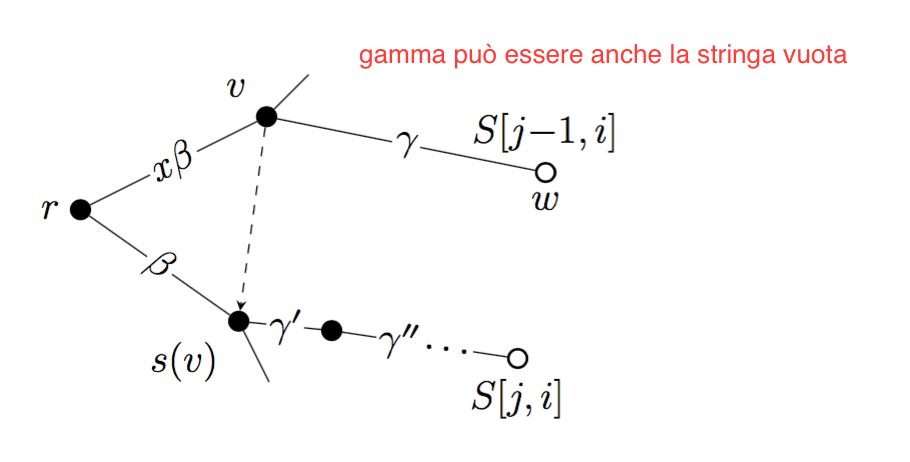
\includegraphics[width=.7\textwidth]{./notes/immagini/l22-fig3.png}
	\caption{La ricerca del suffisso $ S[j,i] $. Si risale, dal nodo con etichetta $ S[j-1,i] = x\alpha = x\beta\gamma $, per al più un arco $\gamma$ fino al nodo $ v $ di etichetta $ x\beta $; ci si muove quindi in $ s(v) $ utilizzando il suffix link e infine si scende il cammino cercando l'arco etichettato $\gamma = \gamma'\gamma''$ per arrivare al nodo di etichetta $ S[j,i] = \beta\gamma =\alpha$.}\label{sadefe2}
\end{figure}

Combinando il tutto l'algoritmo per l'estensione di un suffisso diventa:

\begin{enumerate}
	\item Partendo dal nodo $ w $ dove termina il suffisso $ S[j,i] $ e risalendo verso la radice, cerca il primo nodo esplicito \textit{v} che o ha un suffix link oppure è la radice. Per i corollari precedenti richiede di risalire al massimo di un solo arco.
	
	Sia $\gamma$ l'etichetta, eventualmente nulla, del cammino dal nodo \textit{v} al nodo \textit{w}.
	
	\item Se \textit{v} non è la radice spostati su  $s(v)$ usando il suffix link e quindi discendi seguendo il cammino individuato dalla stringa $ \gamma $.
	
	Se \textit{v} è la radice segui il cammino individuato dalla stringa $ S[j+1,i] $ come per l'algoritmo ingenuo.
	
	\item Estendi il suffisso $ S[j+1,i] $ usando il caso appropriato.
	
	\item Se il nodo \textit{w} è un nodo interno esplicito creato durante l'estensione del suffisso precedente $S[j,i]$ (usando il caso 2), per il lemma 5.4 la stringa $ S[j+1,i] $ deve terminare in un nodo $ s(w) $ esplicito dopo l'estensione di $ S[j+1,i] $. In questo caso metti un suffix link da $ w $ a $ s(w) $
\end{enumerate}

Inoltre, mantenendo un puntatore alla foglia relativa al suffisso più lungo $ S=[1,i] $, la prima estensione della fase \textit{i}-esima non richiede alcuna ricerca e può essere fatta direttamente con il caso 1.

Nonostante ciò la complessità asintotica nel caso pessimo, con una stringa composta da tutti caratteri diversi, non migliora e risulta essere $ O(n^3) $.

\subsubsection{Skip - count}

Durante il secondo passo l'algoritmo discende dal nodo $s(v)$ al cammino di etichetta $\gamma$ e se questo viene fatto normalmente richiede un tempo proporzionale alla lunghezza di $\gamma$.

Sia $g = |\gamma|$ la lunghezza della stringa $\gamma$. Sappiamo che esiste un cammino etichettato con $\gamma$, che può essere anche nullo.

Se $g = 0$, il nodo $s(v)$ è proprio il nodo d'interesse, altrimenti, siccome tutti gli archi uscenti da $s(v)$ hanno etichette che iniziano con caratteri distinti, la scelta dell'arco lungo cui scendere richiede soltanto il confronto con il primo carattere di $\gamma$.

Sia $b$ la lunghezza dell'arco $\beta$ prescelto, tale lunghezza può essere memorizzata assieme all'etichetta.

\begin{itemize}
\item Se $b \leq g$ l'algoritmo non deve controllare nessun altro carattere di $\beta$, perché $\beta$ è certamente uguale al prefisso di $\gamma$ di lunghezza $b$, ossia $\gamma = \beta\gamma'$. L'algoritmo si sposta quindi direttamente sul nodo finale dell'arco prescelto per continuare la ricerca del cammino etichettato $\gamma'$.
\item Se $b > g$ il cammino etichettato $\gamma$ termina nel nodo implicito $g$-esimo di tale arco.
\end{itemize}

Assumendo quindi costante la dimensione dell'alfabeto, ogni spostamento da un nodo esplicito ad un altro nodo lungo il cammino etichettato $\gamma$ richiede un tempo costante.

Il \textbf{livello} $l(v)$ di un nodo esplicito \textit{v} è definito come il numero di archi del cammino dalla radice a \textit{v} o, equivalentemente, come il numero di nodi espliciti che precedono \textit{v} in tale cammino.

Si ha quindi che durante l'esecuzione dell'algoritmo di Ukkonen, viene attraversato un suffix link da $v$ a $s(v)$, vale il \textbf{Lemma 5.7}:

$$
l\big(s(v)\big) \geq l\big(v\big) -1
$$

Questo perché ogni nodo esplicito che precede \textit{v}, esclusa la radice, ha un suffix link che punta ad un nodo che precede $s(v)$. Infatti se l'etichetta del cammino di $v$ è $x\beta$, prefisso del suffisso precedente $S[j,i]$, l'etichetta di cammino di $s(v)$ è $\beta$, prefisso del suffisso $S[j+1,i]$.

Usando quindi lo skip/count, ogni fase dell'algoritmo di Ukkonen richiede tempo $O(n)$.

Infatti, nella fase $i$-esima vengono effettuate $i+1$ estensioni. In ogni estensione l'algoritmo risale al più di un solo arco per trovare il nodo con suffix link, attraversa il suffix link, discende un certo numero di archi e quindi applica uno dei tre casi per l'estensione del suffisso ed eventualmente aggiunge un suffix link. Tutte queste operazioni possono essere fatte in tempo costante, tranne la discesa che dipende dal numero di archi percorsi.

Consideriamo come varia il livello corrente $l$ durante una fase, ossia il livello dell'ultimo nodo esplicito visitato dall'algoritmo.
L'estensione del primo suffisso non modifica $l$ perché applica il caso 1 sul suffisso più lungo.

Ad ogni estensione successiva, \textit{l} diminuisce al più di una unità nella risalita, diminuisce al più di una unità attraversando il suffix link ed aumenta di una unità ogni volta che si discende un arco. Quindi durante l'intera fase \textit{l} può diminuire al più $2i$ volte.

Siccome $l$ rimane sempre $\leq i$, ogni arco ha un'etichetta di almeno un carattere e le etichette sono lunghe al massimo $i$), esso non può aumentare più di $3i$ volte e quindi il numero totale di archi discesi in tutta la fase è al più $3i = O(n)$.

Ricapitolando:
\begin{itemize}
	\item Estendere un suffisso con uno dei 3 casi viene fatto in tempo costante, l'importante è trovare cammino dell'albero da estendere
	\item Utilizzando il suffix-link e lo skip/count ogni fase, l'estensione dell'albero dei suffissi $I_i$ per la stringa $S[1,i]$ nell'albero dei suffissi $I_{i+1}$ per la stringa $S[1,i+1]$, può essere fatta in $O(n)$, questo perché entrambi gli accorgimenti velocizzano la ricerca dei cammini e il numero di archi discesi durante la fase è al massimo $3i = O(n)$.
	\item Per ottenere l'albero dei suffissi per la stringa sono necessarie $n$ fasi.
\end{itemize}

In tutto si ha una complessità di $O(n^2)$.

\subsubsection{Il problema dello spazio}

Al momento l'albero dei suffissi può richiedere uno spazio $O(n^2)$ e ovviamente non può essere costruito in $O(n)$.

Questa occupazione in spazio deriva dal fatto che, anche se i nodi dell'albero non possono essere più di $2n-1$, la somma delle lunghezze delle etichette può richiedere $O(n^2)$. I nodi dell'albero sono le $n$ foglie ed al più $n-1$ nodi interni (perché ogni nodo ha almeno due figli). Nel caso di una stringa con tutti i caratteri distinti, l'albero dei suffissi è costituito soltanto dalla radice e dalle $n$ foglie e la somma delle lunghezze delle etichette è $\sum_{i=1}^n i = O(n^2)$.

La soluzione è quindi quella di rappresentare l'etichetta di un arco con una coppia di indici $(p,q)$ tale che l'etichetta sia $\beta = S[p,q]$, resta inoltre possibile calcolare la lunghezza per effettuare lo skip count con $b = q -p+1$.

Utilizzando le coppie di indici lo spazio richiesto per memorizzare un'etichetta diventa costante.

\subsubsection{Limitazione delle fasi}

Si può osservare che non appena in una fase viene applicato il caso 3, questo viene applicato anche a tutte le successive estensioni della stessa fase.

Questo perché, se viene applicato il caso 3 per l'estensione del suffisso $S[j,i]$ significa che il suffisso $S[j,i+1]$ è già presente nell'albero corrente e quindi sono presenti anche tutti i suffissi successivi da $S[j+1,i+1]$ ad $S[i+1,i+1]$.
Ovvero quando viene applicato il caso 3 vuol dire che all'interno dell'albero è già stato inserito il suffisso $S[j',i+1]$ che ha come prefisso $S[j,i+1]$ per $j' < j$.

Si ha quindi che non appena viene applicato il caso 3, la fase di estensione dell'albero può terminare.

Inoltre, se ad un certo punto dell'algoritmo di Ukkonen viene creata una foglia etichettata \textit{j} per inserire il suffisso $S[j,i+1]$ (caso 2) tale foglia rimane una foglia in tutti i successivi alberi costruiti dall'algoritmo, questo perché l'algoritmo non estende mai un cammino oltre la foglia che lo termina. Quindi tutte le estensioni successive del suffisso associato a tale foglia verranno sempre fatte applicando il caso 1.

L'esecuzione di una fase dell'algoritmo quindi procede sempre secondo un determinato schema:

\begin{enumerate}
	\item La foglia 1 viene costruita nella fase 1, quindi ogni fase inizia con un'estensione che usa il caso 1.
	\item Vengono poi eseguite delle estensioni che usano i casi 1 e 2
	\item Termina non appena viene eseguito il primo caso 3.
\end{enumerate}

Sia $j_{i-1}$ l'ultima estensione che usa i casi 1 o 2 nella fase $(i-1)$-esima. Siccome ogni applicazione del caso 2 crea una nuova foglia, alle prime $j_{i-1}$ estensione della fase successiva si applica il caso 1, per quanto precedentemente osservato.

Dunque per la fase successiva si avrà $j_i \geq j_{i-1}$ e questo ci suggerisce di cercare un trucco che faccia evitare, nella fase successiva, le prime $j_{i-1}$ estensioni che utilizzano il caso 1.

Si può osservare che il caso 1 si limita ad aggiungere all'etichetta dell'arco che termina nella foglia di etichetta $S[j,i]$ il carattere $S[i+1]$.
Quando viene creata una foglia con il caso 2 nella fase $i$-esima all'arco che termina nella foglia viene assegnato solamente il carattere $S[i+1]$ come etichetta. 
Da quel momento in poi l'etichetta verrà via via allungata di un carattere per ogni fase, fino a diventare $S[i+1,n]$.

Si può quindi assegnare, alla creazione della foglia come caso 2, l'etichetta $S[i+1,n]$, sempre se la stringa è nota a priori. Se questo non lo è come coppia che identifica l'etichetta è possibile utilizzare il valore $(i+1,e)$.

Così facendo le prime $j_{i-1}$ estensioni nella fase $i$-esima, non richiedono alcuna operazione e possono essere saltate, iniziando all'estensione $(j_{i-1}+1)$-esima. La fase $i$-esima inizia quindi con l'estensione $j = i_{j-1}+1$ e termina con la prima estensione che usa il caso 3 oppure quando tutti i suffissi sono stati estesi (in questo caso si ha $j = i+2$).

Il valore per la fase successiva risulta essere $j_i = j-1$, ovvero l'ultima posizione che non è stata estesa con il caso 3.

\begin{figure}[htbp]
	\centering
	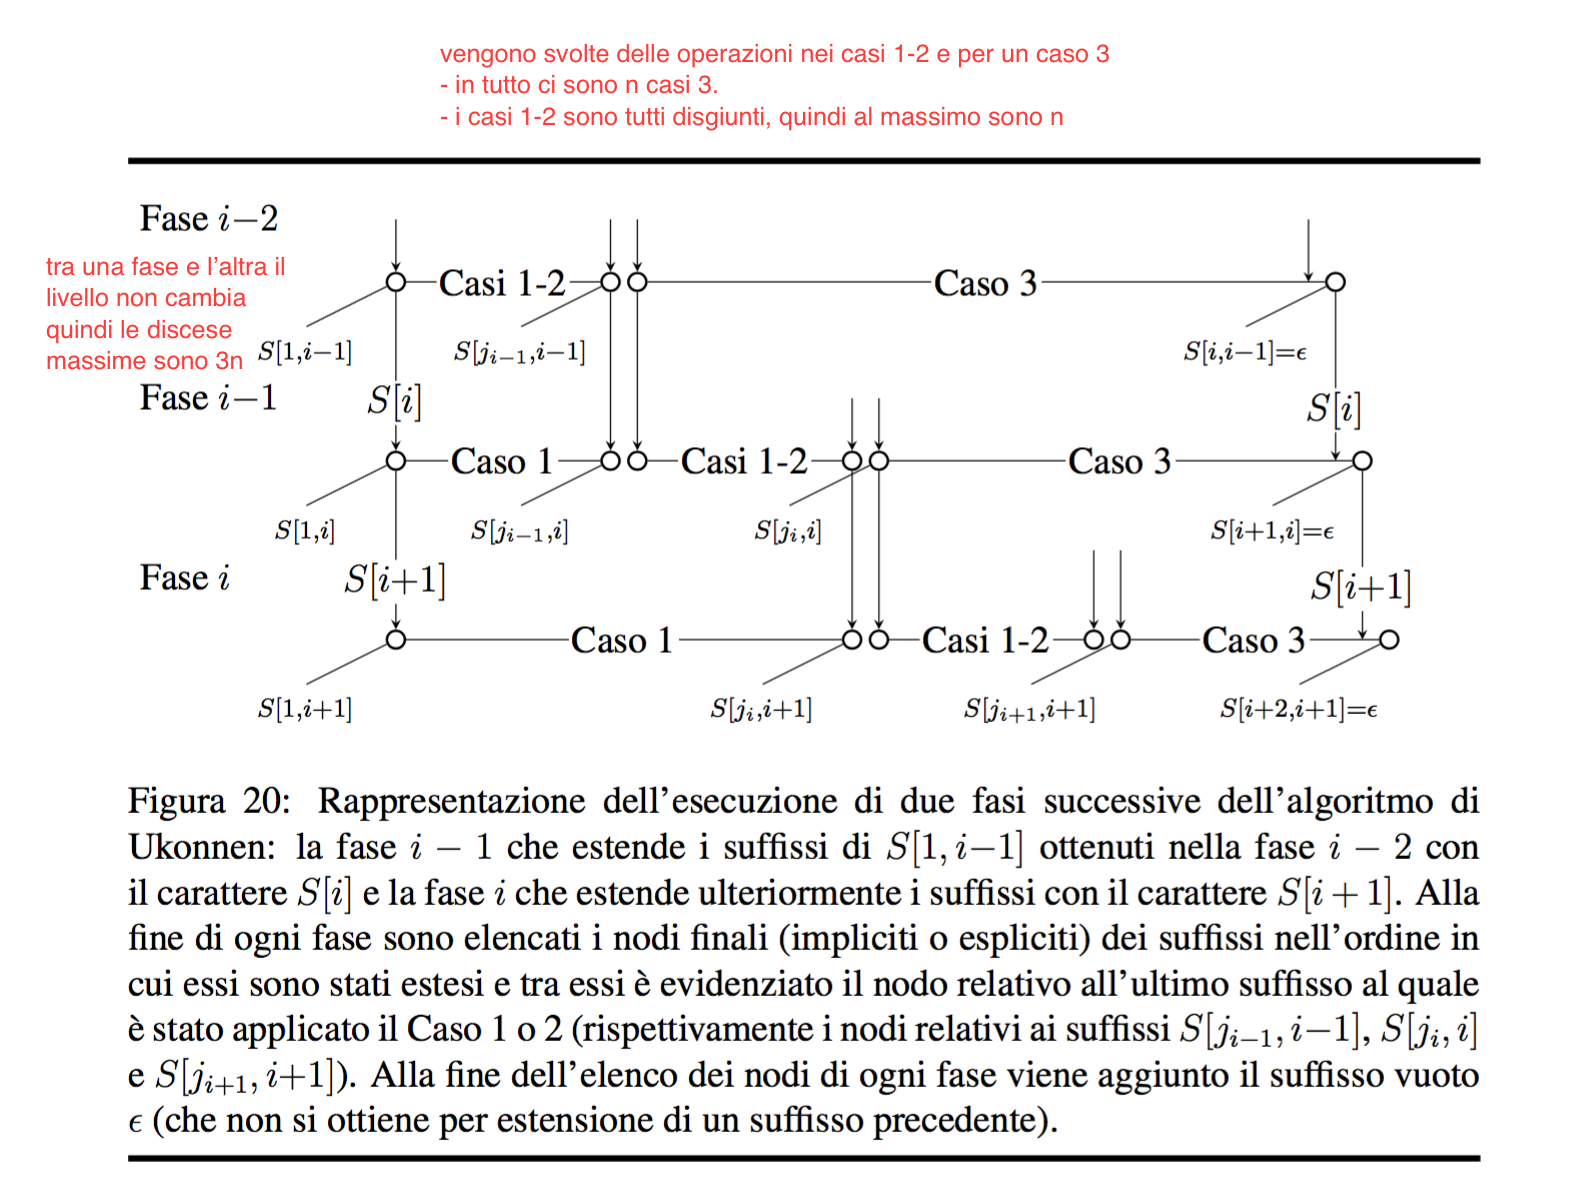
\includegraphics[width=.9\textwidth]{./notes/immagini/l22-fig8.png}
\end{figure}

\paragraph{Dimostrazione del tempo di esecuzione costante}

Se $S[j*, i-1]$ è l'ultimo suffisso esteso nella fase $(i-1)$-esima, la fase $i$-esima inizia con l'estensione del suffisso $S[j*,i]$. Dunque soltanto il suffisso $j*$-esimo viene esteso sia nella fase $(i-1)$-esima che nella fase $i$-esima.

Siccome gli indici $j$ dei suffissi sono tutti minori o uguali ad $n$ e le fasi sono $n$, in totale vengono eseguite al più $2n$ estensioni durante tutta l'esecuzione dell'algoritmo, con ogni estensione che richiede un tempo costante più un tempo proporzionale al numero di archi discesi nella ricerca di $\gamma$, che è un $O(n)$.

Siccome la fase $i$-esima inizia con il suffisso $j*$-esimo in cui è avvenuta l'ultima estensione della fase precedente, il livello corrente non cambia passando da una fase alla successiva (anche nel caso in cui $j_{i-1}=i$, il livello corrente quando si è esteso l'ultimo suffisso $S[i,i-1] = \epsilon$ nella fase $(i-1)$-esima era 0, uguale al livello corrente quando si estende il primo suffisso $S[i+1,i] = \epsilon$ nella fase $i$-esima).

Dunque il fatto che il livello corrente non diminuisca mai più di due volte vale sia all'interno di una singola fase che per tutto l'algoritmo e siccome il livello rimane sempre compreso tra 0 e $n$, il numero di archi discesi durante tutta l'esecuzione dell'algoritmo deve essere minore o uguale a $3n$.

Questo perché nella stessa fase, per quanto precedentemente dimostrato, il livello diminuisce al più di due volte e tra una fase e l'altra il livello non cambia.

Siccome durante tutta l'esecuzione dell'algoritmo vengono eseguite al più $2n$ estensioni ciascuna delle quali richiede un tempo costante più un tempo proporzionale agli archi discesi e il numero totale di archi discesi è minore o uguale a $3n$ si può concludere che l'algoritmo richiede un tempo $O(n)$. Questo perché nelle $2n$ estensioni vengono discesi al massimo $3n$ archi, si ha quindi come complessità $O(2n)+ O(3n) = O(n)$.

Se la lunghezza della stringa non è nota a priori, una volta completata l'esecuzione è necessario andare a correggere le etichette delle foglie.

L'algoritmo di Ukkonen quindi, costruisce on-line l'albero dei suffissi di una stringa di lunghezza $n$ in $O(n)$.
% !TEX encoding = UTF-8
% !TEX TS-program = pdflatex
% !TEX root = computabilità e algoritmi.tex
% !TEX spellcheck = it-IT
\chapter{Algoritmi multithread}\label{algoritmi-multithread}

Finora abbiamo visto solamente algoritmi sequenziali, ma il progresso ha fornito la possibilità di eseguire algoritmi paralleli.

Il problema è che non c'è un modello di calcolo preciso. 
Tipicamente ci sono più processori con della memoria condivisa, oppure ci sono dei cluster composti da processori, ognuno con la propria memoria che comunica con altri cluster per condividere i dati.

Noi ci limiteremo al caso con più processori con memoria condivisa.

In questo caso il lavoro deve essere distribuito tra i vari processori, utilizzando dei \textbf{thread}, dei processi logici che vengono assegnati ai vari processori.

Tipicamente una volta che il thread è stato avviato, questo non viene fermato e rimane in esecuzione su quel processore fino alla fine (\textbf{thread statico}).

La gestione dei thread viene effettuata in modo automatico (\textbf{threading dinamico}) perché lasciarla allo sviluppatore è troppo pericoloso. 
Con questa modalità, il programmatore può specificare quali parti del programma possono essere eseguite in parallelo, la suddivisione del programma in thread viene lasciata alla \textbf{piattaforma parallela} i quali vengono poi assegnati ai vari processori.

L'assegnazione viene effettuata con uno scheduler che cerca di bilanciare il lavoro svolto dai vari processori.

\section{Il primo algoritmo parallelo}\label{il-primo-algoritmo-parallelo}

Come notazione per lo pseudo codice utilizzeremo:

\begin{itemize}
\item
  \textbf{spawn}: posta davanti ad un istruzione indica che questa può essere eseguita in parallelo rispetto al resto del programma. In altre parole segnala che l'istruzione può essere eseguita su un altro thread.
\item
  \textbf{sync}: segnala che è necessario aspettare la terminazione di tutti i thread attivati con spawn.
\item
  \textbf{parallel}: specifica che il corpo di un ciclo \texttt{for} può essere eseguito in modo parallelo.
\end{itemize}

L'istruzione \textbf{spawn} non obbliga il sistema ad eseguire il codice in parallelo, è il sistema che sceglie se conviene o meno.

Se da un programma parallelo togliamo tutte queste istruzioni, otteniamo un classico programma sequenziale.

\subsection{Fibonacci ricorsivo}\label{fibonacci-ricorsivo}

\begin{breakablealgorithm}
\caption{P-Fib: fibonacci in versione parallela}
\begin{algorithmic}[1]
\Function{P-Fib}{n}
\If{$n \leq 1$}
    \State \Return $n$
\EndIf
\State $x \gets \textbf{ spawn } \textsc{P-Fib}(n-1)$ 
\State $y \gets \textsc{P-Fib}(n-2)$
\State $\textbf{sync}$
\State \Return $ x + y$
\EndFunction
\end{algorithmic}
\end{breakablealgorithm}

La complessità per la \textbf{versione sequenziale} di questo codice è proporzionale al numero ritornato dalla funzione, il quale cresce esponenzialmente.

\subsection{Grafo di computazione}\label{grafo-di-computazione}

L'esecuzione di un algoritmo multithread può essere rappresentata con un DAG.

Come prima cosa è necessario individuare gli \textbf{strand} ovvero le porzioni di codice che vengono eseguite in modo sequenziale.

Come notazione per il grafo viene utilizzato:

\begin{itemize}
\item
  \textbf{nero} o un pallino pieno per indicare uno strand.
\item
  \textbf{grigio} o un pallino con una crocetta per indicare la porzione di codice che c'è tra una \textbf{spawn} e una \textbf{sync}.
\item
  \textbf{bianco} o un pallino vuoto per indicare l'istruzione di
  ritorno per un thread (o funzione).
\end{itemize}

\begin{figure}[htbp]
\centering
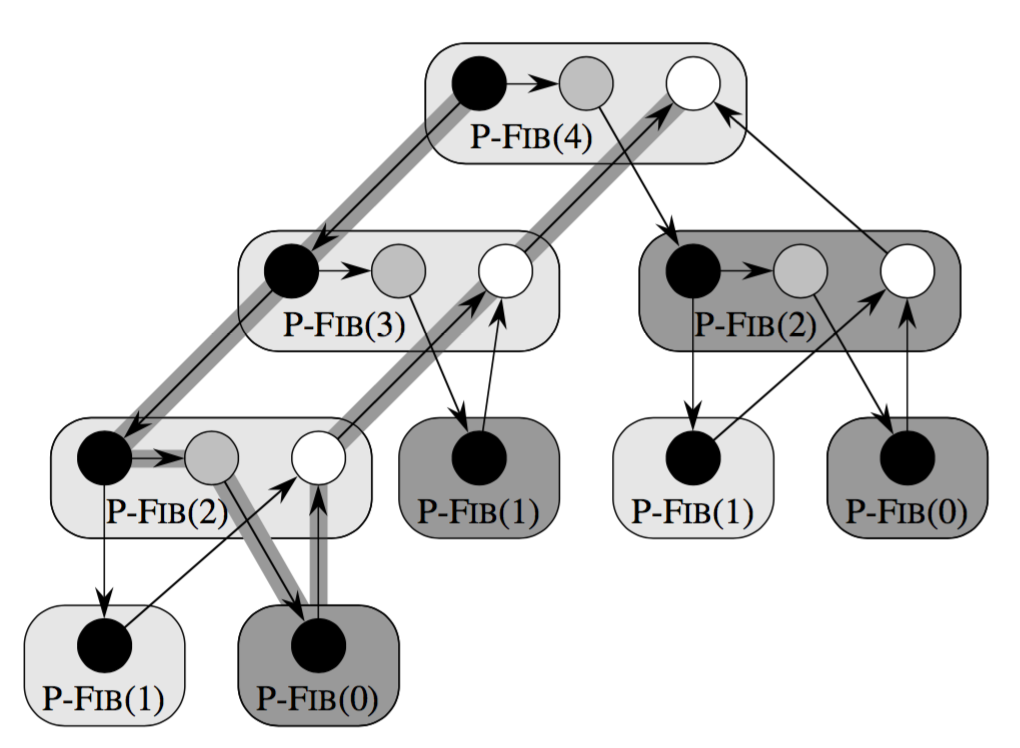
\includegraphics[width=.6\textwidth]{./notes/immagini/l24-fig1.png}
\caption{DAG per \textsc{P-Fib}(4)}
\end{figure}

Nel DAG sopra riportato gli archi hanno vari significati:

\begin{itemize}
	\item \textbf{archi di continuazione}: sono quelli orizzontali che connettono uno strand a quello successivo all'interno della stessa procedura.
	\item \textbf{archi di spawn}: sono quelli che vanno verso il basso e rappresentano il fatto che uno strand ha richiesto lo spawn di un altro strand.
	\item \textbf{archi di chiamata}: anche questi vanno verso il basso e rappresentano l'invocazione di un'altra funzione. Nel grafico fatto dal professore rimangono interni allo stesso blocco.
	\item \textbf{archi di ritorno}: sono quelli che vanno verso l'alto e rappresentano la terminazione di una funzione.
\end{itemize}

\begin{figure}[htbp]
	\centering
	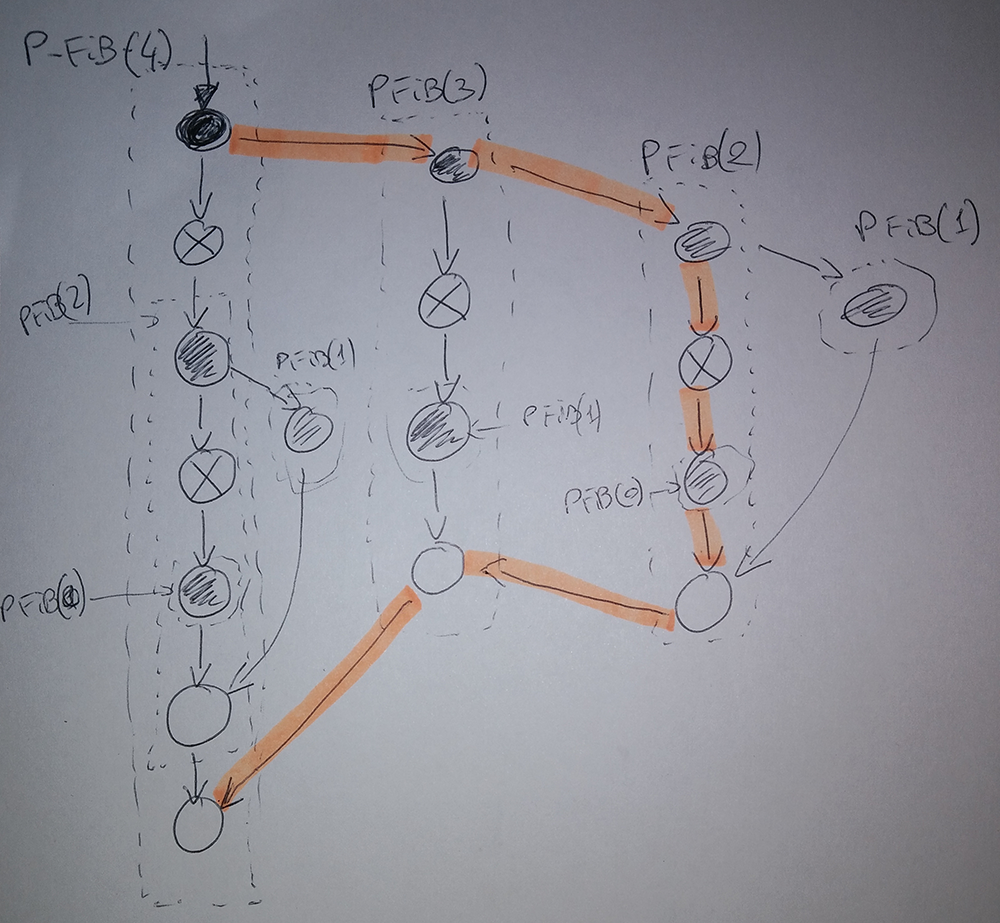
\includegraphics[width=.6\textwidth]{./notes/immagini/l24-alt.png}
	\caption{DAG per \textsc{P-Fib}(4) rappresentato come ha fatto il prof. Anziché evidenziare le chiamate delle funzioni, vengono evidenziati i possibili thread.}
\end{figure}

\subsection{Metriche per la complessità}\label{metriche-per-la-complessituxe0}

Per quanto riguarda la complessità asintotica possiamo considerare che l'esecuzione di uno strand avvenga in tempo costante.

Vengono poi distinte due misure: il \textbf{lavoro} ovvero il numero di strand e la \textbf{durata} (span) che è la lunghezza del cammino massimo (critico) del DAG, ovvero il numero di strand che devono per forza essere eseguiti in sequenza.

Nell'esempio di Fibonacci, il lavoro è 17 e la durata è 8 unità di tempo.

Ovviamente se l'algoritmo viene eseguito in modo sequenziale, il lavoro coincide con la durata ($T_1$). 
Se invece si hanno a disposizione infiniti processori, la durata è il tempo minimo richiesto ($T_\infty$). 

Infine, se si hanno a disposizione \emph{P} processori, valgono:

\begin{itemize}
	\item \textbf{legge del lavoro}: $T_P \geq \frac{T_1}{P}$ che deriva dal fatto che idealmente un computer con \textit{P} processori in $T_P$ riesce a produrre un lavoro pari a $P T_P$
	\item \textbf{legge della durata}: $T_P \geq T_\infty $ che deriva dal fatto che un computer con $P$ processori non può andare più veloce di un computer con processori illimitati.
\end{itemize}

Lo \textbf{speedup} di un algoritmo misura quanto viene velocizzato l'algoritmo utilizzando \emph{P} processori al posto di uno solo: 

$$\textbf{speedup} = \frac{T_1}{T_P} \leq P$$

Se lo speedup è molto più piccolo di \emph{P} non è conveniente aumentare il numero di processori.

Lo speedup viene detto \textbf{lineare} se

$$\frac{T_1}{T_P} = O(P)$$

e \textbf{perfetto} se

$$\frac{T_1}{T_P}  = P$$

Un'altra misura è data dal \textbf{parallelismo} che è il rapporto tra $T_1$ e $T_\infty$ e misura il lavoro medio che può essere eseguito in parallelo, fornendo un limite superiore per lo speedup.

Il parallelismo fornisce anche un limite allo speedup perfetto, ovvero supponendo di avere un numero di processori molto più grande del parallelismo ($P > T_1 / T_\infty$):

$$
T_1/T_P \leq T_1/T_\infty < P
$$

e quindi se 

$$P \gg \frac{T_1}{T_\infty} \quad \text{ allora } \quad \frac{T_1}{T_P} \ll P$$

più processori si hanno rispetto il parallelismo, peggiore è lo speedup. Questo perché avere un numero di processori maggiori rispetto al parallelismo implica che alcuni di questi rimarranno inattivi, ovvero non contribuiscono ad abbassare $T_P$.

Il \textbf{lasco} del parallelismo viene definito come

$$\frac{T_1/T_\infty}{P}$$

ovvero di quanto il parallelismo è maggiore del numero di processori.

Se il lasco è minore di 1, si ha che 

$$\frac{T_1}{T_P} \leq \frac{T_1}{T_\infty} < P$$

e quindi lo speedup non potrà mai essere perfetto. 

Se invece il lasco è maggiore di 1, ci si può avvicinare allo speedup perfetto.

\subsection{Lo scheduling dei thread}\label{lo-scheduling-dei-thread}

L'ordine ottimo che minimizza la durata dell'algoritmo è dato dall'ordinamento topologico del DAG, ma dal momento che il DAG non è noto a priori, non è possibile calcolarlo.

Lo scheduler più semplice è quello \textbf{goloso}, il quale assegna il maggior numero possibile di strand ai processori che ha a disposizione. Se ci sono più strand che thread, la scelta degli strand da assegnare viene fatta casualmente.

Se tutti i thread sono in esecuzione si verifica un passo \textbf{completo} ovvero tutti i processori stanno lavorando. 
Se non ci sono strand a sufficienza per tenere impegnati tutti i processori si ha un passo \textbf{incompleto}. 
Si ottiene così una durata che è pari alla somma dei passi completi e di quelli incompleti.

\subsubsection{Durata di un algoritmo con lo scheduler goloso}

Usando lo scheduler goloso è sempre vero che:

$$T_P \leq \frac{T_1}{P} + T_\infty$$

Il numero di passi completi è $\leq \frac{T_1}{P}$, perché se per assurdo non lo fosse, verrebbe eseguito più lavoro di quanto necessario:

\begin{align*}
\underbrace{P \cdot \bigg(\bigg\lfloor \frac{T_1}{P}\bigg\rfloor +1 \bigg)}_{\text{lavoro svolto dai passi completi assumendo di farne più del necessario}} &= P \bigg( \frac{T_1}{P} - (T_1 \mod P) +1 \bigg) \\
&= T_1 - (T_1 \mod P) + P \\
&> T_1
\end{align*}

 il che è assurdo, perché verrebbe svolto più lavoro del necessario.

Dopo aver eseguito un certo numero di passi completi, verrà eseguito un passo incompleto, quando questo succederà il DAG della computazione sarà un grafo $G'$ che avrà un numero di nodi iniziali (senza dipendenze) minore di \emph{P}, perché il passo è incompleto. 
Per forza di cose, uno di questi nodi appartiene al cammino critico e verrà eseguito, diminuendo di 1 la lunghezza di tale cammino. 
Dal momento che all'inizio la lunghezza del cammino è $T_\infty$, possono esserci al massimo
$T_\infty$ passi incompleti.

Quindi, dato che un passo può essere o completo o incompleto, la durata dell'algoritmo con $ P $ processori è limitata dal numero di passi, ovvero:

$$
T_P \leq \underbrace{\bigg\lfloor \frac{T_1}{P}\bigg\rfloor}_{\text{massimo numero di passi completi}} + \underbrace{T_\infty}_{\text{massimo numero di passi incompleti}}
$$

Questo tipo di scheduler funziona sufficientemente bene dal momento che nel caso peggiore richiede il doppio del tempo rispetto alla schedulazione ottima effettuata conoscendo a priori il DAG, ovvero lo scheduler goloso è \textbf{2-competitivo}.

Sia $T_{P}^*$ il tempo richiesto dallo scheduler ottimo, si ha che per le leggi della durata e del lavoro:

$$T_{P}^* \geq \max \bigg( \frac{T_1}{P} \: , \: T_\infty \bigg)$$

Si ha quindi 

\begin{align*}
T_{P} &\leq T_1/P + T_\infty \\
		 &\leq 2 \cdot \max \bigg( \frac{T_1}{P} \: , \: T_\infty \bigg) \\
		 &\leq 2T_{P}^*
\end{align*}

Inoltre, se $ P \ll T_1 / T_\infty $ si ha che $ T_P \approx T_1/P$, ovvero lo scheduler goloso riesce ad approssimare il parallelismo perfetto al crescere del lasco.

Questo perché se $ P \ll T_1 / T_\infty $ si ha anche che $T_\infty \ll T_1 / P$ e, per quanto precedentemente dimostrato si ha:

$$
T_P \leq \frac{T_1}{P} + T_\infty \approx \frac{T_1}{P}
$$

Quantificando, se un algoritmo ha un lasco di $\cfrac{T_1}{T_\infty P} = 10$, la sua durata $ T_\infty $ è sicuramente $\leq \cfrac{T_1}{10 P}$, ovvero l'algoritmo è 10 volte più parallelo rispetto al numero di processori a disposizione.

$$
T_P \leq \frac{T_1}{T_P} + T_\infty = 1.1 \frac{T_1}{P}
$$

Lo speedup così ottenuto risulta essere quasi perfetto e nella maggior parte dei casi è sufficientemente buono.

Si può quindi aumentare il parallelismo $\cfrac{T_1}{T_\infty}$ se $\cfrac{T_1}{T_\infty} \leq 10 P$  oppure si può diminuirlo se $\cfrac{T_1}{T_\infty} \geq 10 P$.

% !TEX encoding = UTF-8
% !TEX TS-program = pdflatex
% !TEX root = computabilità e algoritmi.tex
% !TEX spellcheck = it-IT

\subsection{Calcolo della durata e del lavoro}\label{calcolo-della-durata-e-del-lavoro}

Il calcolo del lavoro è semplice, basta andare a contare tutte le porzioni di codice sequenziale.

Per calcolare la durata è necessario tenere conto se due attività possono essere eseguite in parallelo

\begin{figure}[htbp]
\centering
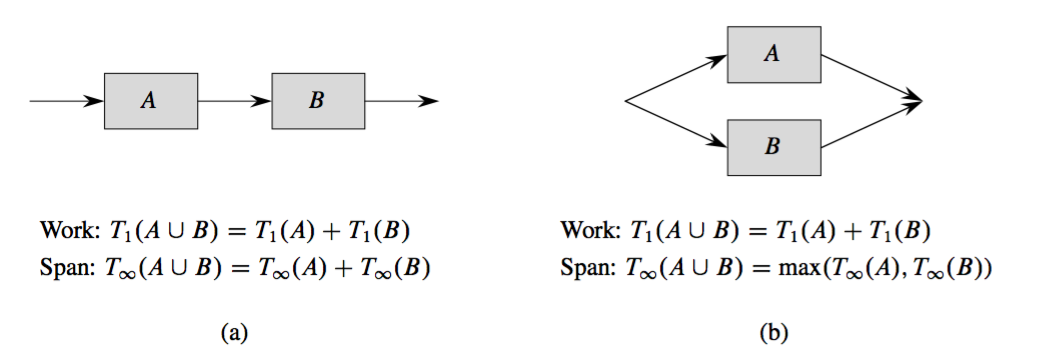
\includegraphics[width=.8\textwidth]{./notes/immagini/l25-fig1.png}
\caption{}
\end{figure}

Se due computazioni devono essere eseguite in sequenza la durata è la somma dei $T_\infty$ delle due compitazioni. Se invece possono essere eseguite in parallelo, la durata è il massimo dei due $T_\infty$.

\subsection{Loop paralleli}\label{loop-paralleli}

Moltiplicazione di un vettore per una matrice di dimensione $n \times n$

\begin{breakablealgorithm}
	\caption{\textsc{MatVec}: Moltiplicazione di una matrice per un vettore}
	\begin{algorithmic}[1]
\Function{MatVec}{$A,x$}
    \State $n \gets A.rows$
    \State $y\gets Vec(n)$
    \State \textbf{parallel}
    \For{$i = 1 \text{ to } n$}
        \State $y_i \gets 0$
    \EndFor
    \State \textbf{parallel}
    \For{$i = 1 \text{ to } n$}
         \For{$j = 1 \text{ to } n$}
            \State $y_i \gets y_i + a_{i,j}x_j$
        \EndFor
    \EndFor
\EndFunction
\end{algorithmic}
\end{breakablealgorithm}


Per quanto riguarda il lavoro si ha $T_1(n) = \Theta(n^2)$.

La durata invece $T_\infty(n)$ si ha che il primo blocco \textbf{parallel} ha durata $\Theta(\log n )$, perché il ciclo di azzeramento viene ottimizzato dalla piattaforma parallela in qualcosa di simile a:

\begin{breakablealgorithm}
\begin{algorithmic}[1]
\Function{Azzera}{$y,i,j$}
\If{$i = j$}
    \State $y_i \gets 0$
\Else 
    \State $m \gets \lfloor (i+j)/2\rfloor$
    \State \textbf{spawn} \textsc{Azzera}$(y,i,m)$
    \State \textsc{Azzera}$(y,m+1,j)$
    \State \textbf{sync}
\EndIf
\EndFunction
\end{algorithmic}
\end{breakablealgorithm}

Il lavoro di questa procedura in funzione di $n = j-i+1$ è $T_1(n)= 2T_1(n/2)+ C = \Theta(n)$. $T_\infty(n)$ è invece uguale a $T_\infty(n/2)+C = \Theta(\log(n))$ che deve essere sommata alla durata del blocco, che in questo caso è costante.

Si ha quindi che quando viene calcolata la durata di un \textbf{parallel for} c'è da tenere in considerazione un $\Theta(\log n )$ dovuto al lavoro svolto dalla piattaforma parallela per parallelizzare le istruzioni.

In modo simile a prima il secondo blocco ha complessità $\Theta(\log n ) +\Theta(n) = \Theta(n)$.

Si ha quindi che quando c'è un parallel c'è sempre una costante $\log n$ da sommare alla complessità a causa dell'implementazione del for.

$T_\infty$ di tutto l'algoritmo è quindi $\Theta(n)$.

\subsection{Race condition}\label{race-condition}

Se l'esecuzione dell'algoritmo fornisce sempre lo stesso risultato viene detto \textbf{deterministico} e questo avviene quando l'ordine di esecuzione degli strand non è influente sul risultato.

Se invece l'ordine è influente sul risultato si ha che l'algoritmo è \textbf{non deterministo} e questo può essere causato da delle \textbf{race condition} ovvero quando due strand eseguiti in parallelo accedono alla stessa locazione di memoria.

Ci sono vari modi per evitare queste situazioni, noi ci limitiamo ad analizzare del codice che non le prevede, ovvero che tutte le operazioni eseguite in parallelo sono tra loro \textbf{indipendenti}.

\subsection{Una lezione di scacchi}\label{una-lezione-di-scacchi}

Un algoritmo parallelo è stato progettato per lavorare con $p = 32$ e con
un $T_{32} = 65 $ secondi.

Si è poi riusciti a ridurre il tempo di esecuzione a $T'_{32} = 40$ secondi.

Tuttavia una volta eseguito il codice con $p = 512$ la seconda versione dell'algoritmo è risultata meno performante.

La versione originale aveva $T_1 = 2048$ e $T_\infty = 1$, mentre quella modificata aveva $T'_1 = 1024$ e $T_\infty = 8$. Ovvero la seconda versione ha dimezzato il lavoro, ma ha aumentato la durata.

Per il programma originale, utilizzando $T_P = T_1/P + T_\infty$:

$$T_{32} = 2048/32 +1 = 65 \quad \text{e} \quad T'_{32} = 1024/32 +8 = 40$$

mentre

$$T_{512} = 2048/512 + 1 = 5 \quad \text{e} \quad  T_{512} = 1024/512 + 8 = 10$$

Morale della favola, diminuire il lavoro non sempre porta ad una riduzione della durata.

\section{Moltiplicazione di due matrici}

\begin{breakablealgorithm}
	\caption{\textsc{P-Square-Matrix-Multiply}: moltiplicazione di due matrici parallelizzata}
	\begin{algorithmic}[1]
		\Function{P-Square-Matrix-Multiply}{A,B}
			\State $n \gets A.rows$
			\State $C \gets n \times n $ Matrix
			\State \textbf{parallel}
			\For{$i = 1 \textbf{ to } n$}
				\State \textbf{parallel}
				\For{$j = 1 \textbf{ to } n$}
					\State $C_{i,j} \gets 0$
					\For{$k = 1 \textbf{ to } n$}
						\State $C_{i,j} \gets C_{i,j} + a_{i,j} \cdot B_{i,j}$
					\EndFor
				\EndFor
			\EndFor
			\State \Return $C$
		\EndFunction
	\end{algorithmic}
\end{breakablealgorithm}

Il lavoro svolto da questo algoritmo è lo stesso delle versione sequenziale, si ha quindi $T_1(n) = \Theta(n^3)$.

Per quanto riguarda la durata, c'è un tempo costante per l'inizializzazione delle matrice, due complessità logaritmiche per i due loop paralleli innestati e un $\Theta(n)$ per il for non parallelo. Si ha quindi:

\begin{align*}
	T_\infty(n) &= O(1) + \Theta(\log n) + \Theta(\log n) + \Theta(n) \\
		&= \Theta(n)
\end{align*}

Il parallelismo è quindi $\Theta(n^2)$ e può essere migliorato utilizzando l'approccio divide-and-conquer del metodo di Strassen.

Da notare che il terzo ciclo for di questo algoritmo non può essere parallelizzato perché altrimenti si creerebbero delle race condition.

\section{Merge Sort}\label{merge-sort}

La versione sequenziale dell'algoritmo prende un array \emph{A} e due indici \emph{p} e \emph{r} e deve ordinare la porzione dell'array compresa tra \emph{p} e \emph{r}.

\begin{breakablealgorithm}
	\begin{algorithmic}[1]
\Function{MergeSort'}{$A,p,r$}
\If{$p < r$}
    \State $q \gets floor(p+r/2)$
    \State \textbf{spawn } \textsc{MergeSort'}$(A,p,q)$
    \State \textsc{MergeSort'}$(A,q+1,r)$
    \State \textbf{sync}
    \State \textsc{Merge}$(A,p,q,r)$
\EndIf
\EndFunction
	\end{algorithmic}
\end{breakablealgorithm}

Il lavoro $T_1(n)$ è $\Theta(n \log n)$ che deriva dalla versione sequenziale del \textsc{MergeSort}.

La durata è invece uguale ad un tempo costante, più la massima durata delle chiamate ricorsive, che possono essere considerate uguali, più la durata del merge, che se viene fatto in modo sequenziale è $\Theta(n)$. 

Si ha quindi che 

$$T_\infty = T_\infty(n/2) + \Theta(n) = \Theta(n)$$ 

(\emph{per il metodo dell'esperto o qualcosa del genere}).

Il parallelismo di questo algoritmo risulta quindi essere $\Theta(\log n)$ che non è buono.

Questo perché nell'ordinamento di un numero elevato di elementi, si riesce a raggiungere uno speedup lineare con pochi processori, ma all'aumentare del numero dei processori l'algoritmo non scala.

Per aumentare il parallelismo è necessario rendere parallela anche la funzione \textsc{Merge}.

\begin{figure}[htbp]
\centering
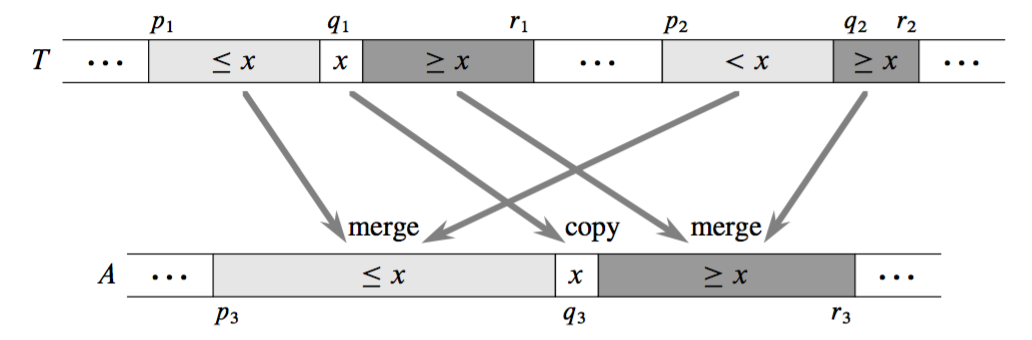
\includegraphics[width=.8\textwidth]{./notes/immagini/l25-fig2.png}
\caption{\textsc{Merge} parallelo}
\end{figure}

Supponiamo che nell'array \emph{T} risultante dalle due chiamate ricorsive ci siano due porzioni ordinate che vanno rispettivamente da $p_1$ a $r_1$ e da $p_2$ a $r_2$.

L'idea è quella di prendere la parte più lunga dei due segmenti. 
Se questa è lunga 0, sono entrambi vuoti e non è necessario fare niente.

Se invece è più lunga di 0, viene calcolato l'indice $q_1$ dell'elemento mediano della prima parte,
ovvero l'elemento centrale della sequenza, il quale avrà un certo valore \emph{x}.

La seconda sequenza può quindi essere divisa in altre due sotto-sequenze, una contenente solo valori minori di \emph{x} e un'altra con tutti i valori $\geq x$. 
Il primo elemento $\geq x$ avrà un certo indice $q_2$ e può essere trovato utilizzando una ricerca binaria in tempo logaritmico.

Da notare che $q_2$ può essere uguale a $p_2$ se sono tutti maggiori uguali di $x$ o a $r_2+1$ se sono tutti minori.

Si sa quindi che, una volta ordinato il vettore, l'elemento \emph{x} si troverà nella posizione $q_3 = p_3 + (q_1-p_1) + (q_2-p_2)$ e può essere già scritto.

Si possono poi unire ricorsivamente tutti gli elementi minori di \emph{x}, ovvero quelli che vanno da $p_1$ a $q_1-1$ e da $p_2$ a $q_2-1$ , e tutti quelli maggiori uguali di $x$, ovvero quelli che vanno da $q_1$ a $r_1$ e da $q_2$ a $r_2$.

Dal momento che i primi andranno a finire nelle posizioni da $q_3$ a $q_3-1$ e i secondi andranno a finire nelle posizioni da $q_3+1$ a $r_3$, le due chiamate ricorsive possono essere parallelizzate.

% !TEX encoding = UTF-8
% !TEX TS-program = pdflatex
% !TEX root = computabilità e algoritmi.tex
% !TEX spellcheck = it-IT
\subsection{Codice del merge parallelo}\label{codice-del-merge-parallelo}

Ci sarebbe prima il codice della ricerca binaria, ma è quella classica
sequenziale e che ritorna l'indice dell'elemento in tempo $O(\log n)$

\begin{breakablealgorithm}
	\caption{\textsc{P-Merge}: merge di due array parallelizzato}
	\begin{algorithmic}[1]
\Function{P-Merge}{$T, p_1, r_1, p_2, r_2, A, p_e$}
    \State $n_1 \gets r_1 - p_1 +1$
    \State $n_2 \gets r_2 - p_2 +1$
    \If{$n_1 < n_2$}
        \State inverti le due parti in modo che $n_1 \geq n_2$
    \EndIf
    \If{$n_1 = 0$}
        \State \Return
    \EndIf
    \State $q_1 \gets \lfloor (p_1 + r_1) / 2 \rfloor$ \Comment{Elemento mediano della prima parte}
    \State $q_2 \gets \textsc{Binary-Search}(T[q_1], T, p_2, r_2)$
    \State $q_3 \gets p_3 + (q_1 - p_1) + (q_2 - p_2)$ 
    \State $A[q_3] \gets T[q_1]$
    \State \textbf{spawn } \textsc{P-Merge}$(T, p_1, q_1 -1, p_2, q_2 -1, A, p_3)$ \Comment{Unisce i valori $\leq x$}
    \State \textsc{P-Merge}$(T, q_1 +1, r_1, q_2, r_2, A, q_3+1)$
    \State \textbf{sync}
\EndFunction
\end{algorithmic}
\end{breakablealgorithm}

\subsubsection{Analisi della complessità}\label{analisi-della-complessituxe0}

La durata $PM_\infty(n)$ del merge è data da una costante per i vari calcoli dell'indice, più un tempo logaritmico per la ricerca binaria, più il tempo delle due chiamate che vengono fatte in parallelo.

La durate delle chiamate parallele dipende dal blocco più grande, ma che dimensione ha?

Ogni chiamata, nella peggiore delle ipotesi viene fatta su $n_1/2 + n_2$ elementi, $n_2$ deriva dal fatto che gli elementi della seconda parte dell'array possono essere tutti minori di $x$ o tutti maggiori uguali.

$$\frac{n_1}{2} +n_2 = \frac{n_1}{2} + \frac{n_2}{2} + \frac{n_2}{2} \leq \frac{n}{2} + \frac{n}{4} = \frac{3n}{4}$$

Si ha quindi che

$$
PM_\infty(n) \leq PM_\infty(\frac{3}{4}n) + O(\log n) = O(\log^2 n)
$$

Per quanto riguarda il lavoro si ha

$$
PM_1(n) = PM_1(\alpha n) + PM_1( (1-\alpha) n) + O(\log n)
$$

perché è dato dalla somma del lavoro delle due parti parallele, più il lavoro necessario per la ricerca binaria.

Per quanto riguarda $\alpha$ si ha che è nel range $1/4 \leq \alpha \leq 3/4$.

Risparmiando i conti, il lavoro finale è dato da

$$
PM_1(n) \leq c_1 - c_2 \log (n) = \Theta (n)
$$

Il parallelismo di questo algoritmo risulta essere buono, perché

$$
\frac{PM_1}{PM_\infty} = \Theta \Big(\frac{n}{\log^2 n}\Big)
$$

e si ottiene uno speedup quasi lineare già per $n$ maggiore di 10.

\subsection{Merge Sort parallelo v2}\label{merge-sort-parallelo-v2}

\begin{breakablealgorithm}
	\caption{\textsc{P-Merge-Sort}: merge sort parallelizzato bene}
	\begin{algorithmic}[1]
\Function{P-Merge-Sort}{$A,p,r, B, S$}
\State $n \gets r - p +1$
\If{$n = 1$}
    \State \Return
\EndIf 
\If{$p < r$}
    \State $T[1 \ldots n] $ nuovo array
    \State $q \gets floor(p+r/2)$
    \State $q' \gets q - p +1$
    \State \textbf{spawn } \textsc{P-Merge-Sort}$(A,p,q, T, 1)$
    \State \textsc{P-Merge-Sort}$(A,q+1,r, T, q'+1)$
    \State \textbf{sync}
    \State \textsc{P-Merge}$(T, 1, q', q'+1, n, B, s)$
\EndIf
\EndFunction
\end{algorithmic}
\end{breakablealgorithm}

Questa versione modificata riceve come parametro anche un'array dove mettere gli elementi una volta ordinati ed esegue le chiamate ricorsive in parallelo.

La differenza sta che una volta sincronizzate le due chiamate, il merge viene fatto con la procedura parallela.

Il lavoro di questa versione è

$$
MS_1(n) = 2 MS_1(n/2) + \Theta(n) = \Theta (n \log n)
$$

che è lo stesso della versione precedente.

La durata invece è

\begin{align*}
MS_\infty (n) &= MS_\infty (n/2) + \Theta(\log^2 n) \\
              &=\Theta (\log^3 n)
\end{align*}

ovvero la durata di una delle due chiamate ricorsive parallele, che tanto sono uguali perché l'array viene diviso a metà, più la durata dell merge ricorsivo.

Anche in questo caso il parallelismo risulta essere

$$
O(\frac{n}{\log^2 n})
$$

\section{P-Scan}\label{p-scan}

Si ha a disposizione un'array e una certa operazione associativa da effettuare sugli elementi dell'array, come la somma di interi, la $and$ tra valori booleani, ecc.

Noi ci concentreremo sulla somma di numeri interi.

Fare questo è facile, ed è facilmente parallelizzabile in modo divide-et-impera, ma una cosa più interessante è quella di creare un nuovo array che contiene gli \emph{step intermedi}:

\begin{align*}
y[1] &= x[1] \\
y[2] &= x[1] + x[2] \\
&\vdots \\
y[n] &= x[1] + \ldots + x[n]
\end{align*}

La versione sequenziale dell'algoritmo può essere quindi definita come

\begin{breakablealgorithm}
\begin{algorithmic}[1]
\Function{Scan}{x}
\State \ldots
\State $y[1] \gets x[1]$
\For{$ i = 2 \textbf{ to } n$}
    \State $y[i]\gets y[i-1] (x) x[i]$
\EndFor
\State \Return $y$
\EndFunction
\end{algorithmic}
\end{breakablealgorithm}

Per parallelizzare questa procedura può essere utile calcolare il valore centrale dell'array.

Prima vediamo il codice:

\begin{breakablealgorithm}
	\caption{\textsc{P-Scan}: funzione principale}
	\begin{algorithmic}[1]
\Function{P-Scan}{$x$}
    \State $y[1] \gets x[1]$
    \If{$n > 1$}
        \State //$t$ è un array temporaneo
        \State \textsc{P-Scan-Up}$(x, t, 2, n)$
        \State \textsc{P-Scan-Down}$(x[1], x, t, y, 2, n)$
    \EndIf
    \State \Return $y$
\EndFunction
\end{algorithmic}
\end{breakablealgorithm}

La procedura \textsc{P-Scan-Up} calcola ricorsivamente la somma della prima metà dell'array e pone il risultato al centro dell'array \emph{t}, dopodiché si invoca ricorsivamente sulla seconda parte dell'array \emph{x}. (Le due invocazioni ricorsive vengono fatte in parallelo).
Quando entrambe le chiamate ricorsive sono terminate, viene ritornata la somma dei due risultati.

Così facendo, vengono calcolati nel vettore di supporto i risultati parziali relativi alla parte sinistra dell'array.

Il nome della procedura deriva dal fatto che prima viene diviso l'array fino ad arrivare ai singoli elementi e poi nella risalita dell'albero delle chiamate vengono effettuati i conti e memorizzati i risultati.

\begin{breakablealgorithm}
	\caption{\textsc{P-Scan-Up}}
	\begin{algorithmic}[1]
\Function{P-Scan-Up}{$x,t,i,j$}
    \If {$i = j$}
        \State \Return $ x[i]$
    \EndIf
   \State $k \gets \lfloor (i+j)/2\rfloor$
   \State $t[k] \gets $ \textbf{spawn} \textsc{P-Scan-Up}$(x,t,i,k)$
    \State $r \gets \: \textsc{P-Scan-Up}(x,t,k+1,j)$
    \State \textbf{sync}
    \State \Return $T[k]+r$
\EndFunction
\end{algorithmic}
\end{breakablealgorithm}

\begin{figure}[htbp]
	\centering
	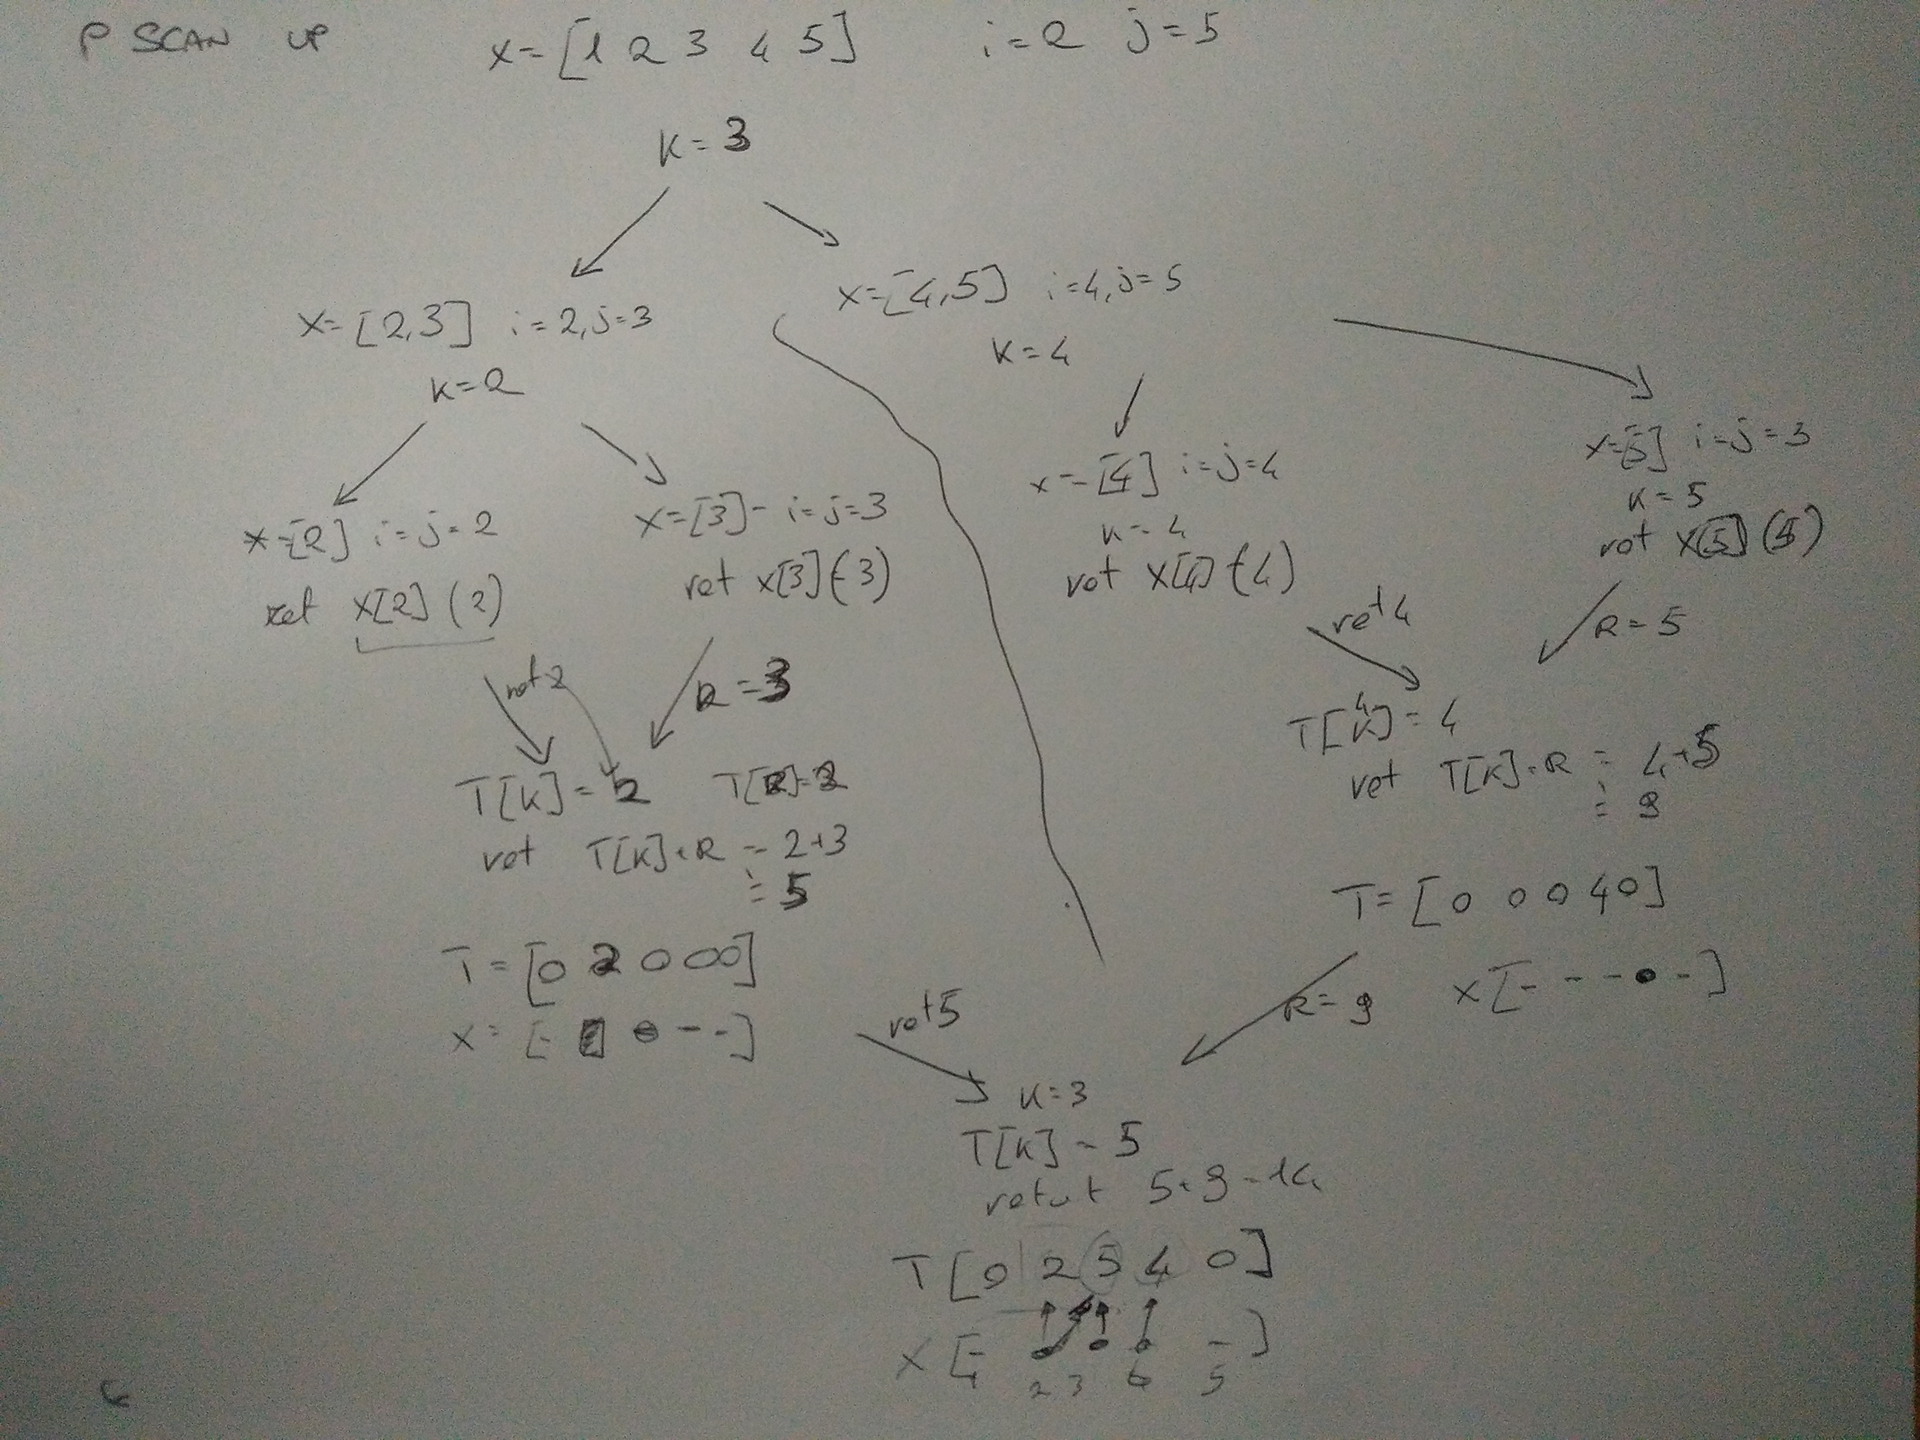
\includegraphics[width=\textwidth]{./notes/immagini/l27-pscanup.png}
	\caption{Albero delle chiamate per \textsc{P-Scan-Up}}
\end{figure}

La funzione \textsc{P-Scan-Down} utilizza le somme parziali prodotte da \textsc{P-Scan-Up} per calcolare e memorizzare nell'array \textit{y} i risultati finali.

Da notare che quando viene invocata la procedura per il calcolo dei valori a destra di $k$ viene utilizzato sia il valore \textit{v} della somma fino ad \textit{i} che il valore $T[k]$ che rappresenta la somma parziale dei valori della parte sinistra.

Anche in questo caso il nome della procedura indica la direzione in cui vengono effettuati i conti, ovvero durante la discesa dell'albero delle chiamate.

\begin{breakablealgorithm}
		\caption{\textsc{P-Scan-Down}}
		\begin{algorithmic}[1]
\Function{P-Scan-Down}{$v,x,t,y,i,j$}
    \State // $ v $ è il valore della somma fino ad $ i $ escluso
    \If{$i=j$}
        \State $y[i] \gets v+x[i]$
    \Else
        \State $ k \gets \lfloor(i+j)/2\rfloor$
        \State \textbf{spawn} \textsc{P-Scan-Down}($v,x,t,i,k$)
        \State \textsc{P-Scan-Down}($v+t[k],x,t,k+1,j$)
        \State \textbf{sync}
    \EndIf
\EndFunction
\end{algorithmic}
\end{breakablealgorithm}

\begin{figure}[htbp]
	\centering
	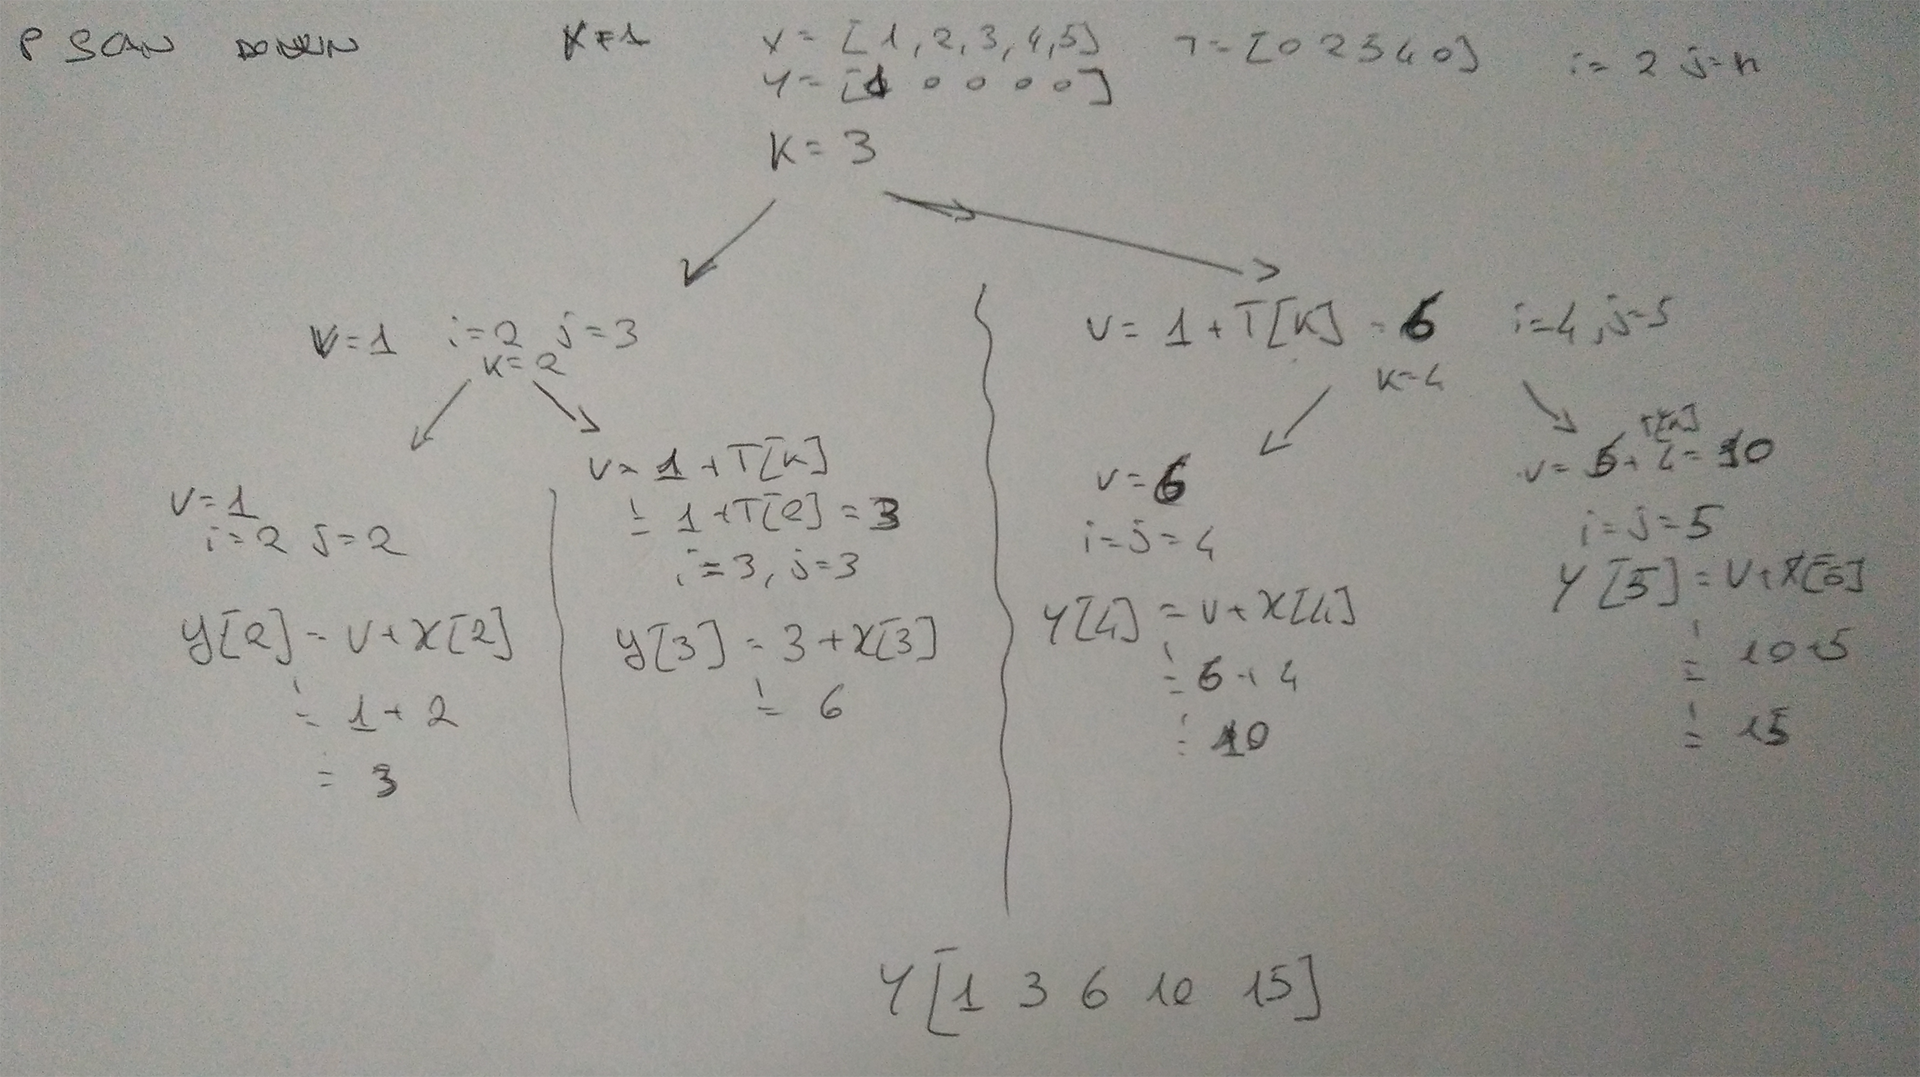
\includegraphics[width=\textwidth]{./notes/immagini/l27-pscandown.png}
	\caption{Albero delle chiamate per \textsc{P-Scan-Down}}
\end{figure}

Combinando le due procedure si ha quindi che le due chiamate parallele di entrambe le procedure lavorano sempre su dati distinti, evitando così delle race condition.

Il lavoro di \textsc{P-Scan} è

$$
T_{1}^{pscan}(n) = T_{1}^{pscan-up}(n) + T_{1}^{pscan-down}(n) + \Theta(1)
$$

e dal momento che anche le due chiamate vengono fatte in modo sequenziale, anche la durata è uguale a

$$
T_{\infty}^{pscan}(n) = T_{\infty}^{pscan-up}(n) + T_{\infty}^{pscan-down}(n) + \Theta(1)
$$

Sia \textsc{P-Scan-Up} che \textsc{P-Scan-Down} hanno la stessa durata e lo stesso lavoro, perché fanno operazioni molto simili, ci concentriamo quindi su \textsc{P-Scan-Up}, tanto la differenza è al più di una costante.

Tenendo a mente che $n = j - i +1 $

$$
T_{1}^{pscan-up}(n) = 2 T_{1}^{pscan-up}(n/2) + \Theta(1) = \Theta(n)
$$

e

$$
T_{\infty}^{pscan-up}(n) = T_{\infty}^{pscan-up}(n/2) + \Theta(1) = \Theta(\log n)
$$

Mettendo assieme i vari pezzi si ha che

$$
T_{1}^{pscan}(n) = 2 T_{1}^{pscan-up}(n) = \Theta(n)
$$

e

$$
T_{\infty}^{pscan}(n) = 2T_{\infty}^{pscan-up}(n) = \Theta(\log n)
$$

Il parallelismo dell'algoritmo risulta essere $\Theta(\frac{n}{\log n})$ che è molto buono.


\subsection{Correttezza dell'algoritmo}

Partiamo dalla funzione \textsc{P-Scan-Down}, la quale dato l'array di partenza e l'array di supporto contente le somme parziali delle varie parti sinistre, calcola nell'array finale il risultato.

La procedura riceve in input in valore \textit{v} con il risultato parziale degli elementi a sinistra della porzione dell'array sul quale viene invocata la procedura. La prima chiamata viene fatta utilizzando il valore in posizione 1, dato che entrambe le procedure iniziano a lavorare dal secondo elemento, perché il primo basta che venga semplicemente ricopiato.

Si ha quindi che se si verifica il caso base, ovvero la procedura viene invocata su un array con un solo elemento, viene effettuata la somma di \textit{v} con il corrispettivo elemento in input, la quale viene poi memorizzata nella corretta posizione dell'array con i risultati. Si ha quindi che il caso base gestito correttamente.

Nel caso ricorsivo, si ha che viene calcolata la posizione centrale dell'array sul quale si sta lavorando e viene invocata ricorsivamente la procedura sulla due parti destre e sinistre. Alla procedura che lavora sulla parte sinistra viene passato come valore di \textit{v} lo stesso ricevuto come parametro, ovvero la somma parziale dei valori che si trovano a sinistra della porzione dell'array sul quale si sta lavorando ed è il valore corretto perché la parte sinistra inizia alla stessa posizione della porzione corrente. Si ha quindi che la procedura ricorsiva sinistra viene invocata correttamente e su una porzione di array inferiore, quindi si può assumere induttivamente che vengano effettuate le operazioni corrette.

Per quando riguarda la parte destra, questa viene invocata con \textit{v} uguale a $v + T[k]$, ovvero la somma parziale della parte \textbf{a sinistra} della porzione corrente più la somma parziale della parte \textbf{sinistra} dell'array corrente e, assumendo che l'array \textit{T} sia stato calcolato correttamente, l'invocazione è corretta e quindi si può assumere induttivamente che vengano eseguiti i calcoli corretti.

Per quanto riguarda \textsc{P-Scan-Up}, si ha che, dato l'array dei valori, deve essere calcolato l'array $T$ contenente le somme parziali, in modo che 

$$
T\big[\lfloor n/2 \rfloor \big] = \sum\limits_{i=1}^{n/2} x[i]
$$

e deve ritornare la somma di tutti gli elementi della porzione dell'array di input che gli è stata fornita.

Nel caso base, con l'array contenente un solo elemento, si ha che il risultato parziale non viene calcolato perché la parte sinistra è vuota e viene ritornato il valore dell'unico elemento dell'array che è uguale alla somma di tutti gli elementi. Si ha quindi che il caso base viene gestito correttamente.

Nel caso ricorsivo, viene calcolato l'elemento mediano ed invocata ricorsivamente la funzione sulle due porzioni dell'array. Dal momento che le invocazioni vengono effettuate su una porzione ridotta dell'array, si può assumere che queste ritorno i valori corretti.
Si ha quindi che in $T[k]$ viene memorizzata la somma parziale della parte sinistra dell'array corrente, che è l'operazione corretta da fare, e che viene ritornato correttamente $T[k]+r$, ovvero la somma dei due parziali delle due parti, cioè la somma di tutti gli elementi dell'array d'invocazione.

Dato che entrambe le funzioni sono corrette, anche \text{P-Scan} è corretta.

\chapter{Geometria computazionale}

Ci sono varie applicazioni della geometria computazionale

Noi ci concentriamo sullo spazio bi-dimensionale.

L'elemento alla base di tutto è il punto, che sarà caratterizzato da due coordinate, le quali saranno tipicamente dei numeri float che sono soggetti a degli errori di arrotondamento.

Ma c'è sempre il piano B, ovvero utilizzare le coordinate intere a 32 bit.

Le nostre coordinate saranno quindi comprese tra un $-$\textsc{Maxint} e \textsc{Maxint}.

C'è però un problema, tipicamente nella geometria computazionale vengono calcolate delle aree, che devono anch'esse essere contenute in un intero e quindi i valori delle coordinate devono essere compresi in un intervallo $-$\textsc{CMax} e \textsc{CMax} con $\textsc{CMax} \leq \sqrt{\textsc{Maxint}} /2$, quindi facendo due conti si ha $\textsc{Maxint} = 2^{31} $ e $\textsc{CMax} = 2^{15}$.

E' poco ma sufficientemente buono, perché su uno schermo di un metro per un metro si ottengono 32 punti per ogni millimetro.

Una volta stabilito come rappresentare i punti si possono rappresentare:

\begin{itemize}
\item   un segmento, utilizzando due punti
\item   un cerchio, con il centro e il raggio
\item   un poligono, con una serie di punti che rappresentano i vertici.
\end{itemize}

Il vettore \emph{v} di coordinate $(v_x, v_y)$ viene rappresentato con uno qualsiasi dei segmenti orientati $\overrightarrow{pq}$ tali
che $v_x = x_q-x_p$ e $v_y = y_q - y_p$.

Talvolta con lo stesso simbolo può essere rappresentato sia il punto di coordinate $(x_p,y_p)$ che il \textbf{vettore posizione} $(x_p,y_p)$ rappresentato dal segmento orientato $\overrightarrow{op}$, dove \textit{o} è l'origine degli assi.

Il \textbf{prodotto vettoriale} di due vettori $v_1 = (x_1,y_1)$ e $v_2 = (x_2,y_2)$ è definito come l'area orientata del parallelogramma dato dai vertici: $o \equiv (0,0)$, $p_1 \equiv (x_1,y_1)$, $q \equiv  (x_1+x_2, y_1+y_2)$ e $p_2 \equiv (x_2, y_2)$.
L'orientamento è positivo se l'angolo da $v_1$ a $v_2$ è orientato in senso antiorario, con segno negativo altrimenti.

\begin{figure}
	\centering
	\includegraphics[width=0.7\textwidth]{./notes/immagini/l27-fig1.png}
	\caption{L'area orientata del parallelogramma individuato dai due vettori $v_1$ e $v_2$.}
\end{figure}

L'area orientata può essere calcolata come il determinate della matrice

$$
v_1 \times v_2 = \det \: \begin{bmatrix}
x_1 & x_2 \\
y_1 & y_2
\end{bmatrix} = x_1 y_2 - x_2 y_1
$$

questo perché l'area del trapezio è uguale a

$$
A = \frac{x_2y_2}{2} + x_1\frac{y_2+(y_1+y_2)}{2} - \frac{x_2y_2}{2} - x_2\frac{y_2+ (y_1+y_2)}{2} = x_1y_2 - x_2y_1
$$

Se cambio l'ordine dei punti, il segno dell'area cambia.

% !TEX encoding = UTF-8
% !TEX TS-program = pdflatex
% !TEX root = computabilità e algoritmi.tex
% !TEX spellcheck = it-IT
\section{I primi problemi semplici:}\label{la-soluzione-ai-semplici-problemi}



\begin{itemize}
	\item
	Dati due segmenti orientati con un vertice in comune, il secondo segmento è ruotato in senso orario o antiorario rispetto il primo?
	\item
	Seguendo il percorso dato da due segmenti orientati, per spostarmi sul secondo devo girare a sinistra o a destra?
	\item
	Due segmenti si intersecano?
\end{itemize}

Abbiamo però il limite che non possiamo utilizzare la divisione e le funzioni trigonometriche perché abbiamo a disposizione solo numeri interi.


\subsection{Rotazione in senso orario o antiorario}\label{rotazione-in-senso-orario-o-antiorario}

In questo caso basta calcolare il prodotto vettoriale

\begin{breakablealgorithm}
	\caption{\textsc{Angle-Left}: angolazione di un segmento rispetto ad un segmento di riferimento}
	\begin{algorithmic}[1]
		\Function{Angle-Left}{$p_0,p_1,p_2$}
			\State $d = (x_1-x_0)(y_2-y_0) - (x_2-x_0)(y_1-y_0)$
			\State \Return $d$
		\EndFunction
	\end{algorithmic}
\end{breakablealgorithm}

\emph{d} risulta essere maggiore di 0 se l'angolo tra i segmenti $\overrightarrow{p_0p_1}$ e $\overrightarrow{p_0p_2}$ è orientato in senso antiorario, se invece è minore di 0 l'angolo è
ruotato in senso orario e se è uguale a 0 l'angolo è 0 oppure uno dei
due segmenti è degenere.

\subsection{Il giro del volante}\label{il-giro-del-volante}

Devo girare a sinistra se tra $\overrightarrow{p_0p_1}$ e il vettore $\overrightarrow{p_0p_2}$ c'è una rotazione in senso antioraria. (Da notare che in questo caso i segmenti di interesse sono $\overrightarrow{p_0p_1}$ e $\overrightarrow{p_1p_2}$).

\begin{breakablealgorithm}
	\caption{\textsc{Turn-Left}: rotazione rispetto ad un segmento}
	\begin{algorithmic}[1]
		\Function{Turn-Left}{$p_0,p_1,p_2$}
			\State $d \gets \textsc{AngleLeft}(p_0,p_1,p_2)$
			\State \Return $d$
		\EndFunction
	\end{algorithmic}
\end{breakablealgorithm}

Se $d >0 $ c'è una svolta a sinistra, se invece è minore di 0 la svolta è a destra e se è 0 si prosegue nella stessa direzione o si fa un'inversione ad U.

\subsection{Intersezione di due segmenti}\label{intersezione-di-due-segmenti}

Si vuole sapere se i due segmenti $\overline{p_1p_2}$ e $\overline{p_3p_4}$ si intersecano o meno.

Ci sono due possibili casi:

\begin{enumerate}
\item
  I due segmenti stanno sulla stessa retta (collineari). In questo caso si intersecano solo se uno dei due estremi $p_3$ o $p_4$ appartiene al segmento $\overline{p_1p_2}$ oppure uno dei due segmenti contiene l'altro.
\item
  I due segmenti non sono sulla stessa retta. In questo caso bisogna vedere se $p_1$ e $p_2$ stanno dalla parte opposta della retta $\overline{p_3p_4}$ e se $p_3$  e $p_4$ stanno dalla parte opposta della retta $\overline{p_1p_2}$.
\end{enumerate}

Per verificare che due segmenti siano collineari basta calcolare il prodotto vettoriale

$$
d_1 = (p_1-p_3) \times (p_4-p_3) \text{// } p_1\text{ rispetto } \overline{p_3p_4}
$$

Se uno dei due segmenti è degenere si ottiene sempre $d_1 = 0$, è necessario quindi verificare che non ci siano segmenti degeneri.

\begin{align*}
d_2 &= (p_2-p_3) \times (p_4-p_3) \text{// } p_2\text{ rispetto } \overline{p_3p_4}\\
d_3 &= (p_3-p_1) \times (p_2-p_1) \text{// } p_3\text{ rispetto } \overline{p_1p_2} \\
d_4 &= (p_4-p_1) \times (p_2-p_1) \text{// } p_4\text{ rispetto } \overline{p_1p_2}
\end{align*}

Se $d_1 = d_2 = 0$ o i due segmenti sono sulla stessa retta o $\overline{p_3p_4}$ è degenere. 
Se $d_3=d_4=0$ o i due segmenti sono sulla stessa retta o $\overline{p_1p_2}$ è degenere.

Basta quindi calcolare i 4 prodotti scalari e controllare se sono tutti 0. In caso affermativo si ha che i due segmenti sono collineari ed è corretto anche se entrambi i segmenti sono degeneri perché due segmenti degeneri sono anche collineari. Per verificare se i due segmenti si intersecano basta quindi controllare se $p_3$ o $p_4$ sono interni da $\overline{p_1p_2}$ oppure se $\overline{p_1p_2}$ è interno a $\overline{p_3p_4}$.

Se almeno uno dei prodotti scalari è diverso da $0$ si ha che i segmenti non sono collineari. In questo caso, se $d_1$ e $d_2$ hanno segno opposto, i punti $p_1$ e $p_2$ si trovano dalla parte opposta rispetto a $\overline{p_3p_4}$ e quindi intersecano internamente la retta che passa per il segmento. Se invece $d_1$ o $d_2$ sono uguali a 0, o $\overline{p_3p_4}$ è degenere, oppure uno dei due punti si trova sulla retta passante per $\overline{p_3p_4}$.
Resta quindi da controllare la posizione di $p_3$ e $p_4$ rispetto a $\overline{p_1p_2}$ e questo viene fatto nello stesso modo.

\begin{breakablealgorithm}
	\caption{\textsc{Segment-Intersect}: due segmenti si intersecano?}
	\begin{algorithmic}[1]
		\Function{Segment-Intersect}{$p_1,p_2,p_3,p_4$}
		    \State $d_1 \gets \textsc{Angle-Left}(p_3,p_4,p_1)$
		    \State $d_2 \gets \textsc{Angle-Left}(p_3,p_4,p_2)$
		    \State $d_3 \gets \textsc{Angle-Left}(p_1,p_2,p_3)$
		    \State $d_4 \gets \textsc{Angle-Left}(p_1,p_2,p_4)$
		    \If{$d_1 = d_2 = d_3 = d_4 = 0$} \Comment{Caso con segmenti collineari}
		        \State \Return $((x_2 - x_3)(x_1 - x_3) \leq 0 \textbf{ and } (y_2 - y_3)(y_1 - y_3) \leq 0) \textbf{ or } \text{// }p_3 \text{ in } \overline{p_1p_2}$
		        \Statex $\qquad \qquad \qquad((x_2 - x_4)(x_1 - x_4) \leq 0 \textbf{ and } (y_2 - y_4)(y_1 - y_4)\leq 0) \textbf{ or } \text{// }p_4 \text{ in } \overline{p_1p_2}$
		        \Statex $\qquad \qquad \qquad ((x_4 - x_1)(x_3 - x_1) \leq 0 \textbf{ and } (y_4 - y_1)(y_3 - y_4)\leq 0) \text{ // }p_1 \text{ in } \overline{p_3p_4} $\Comment{serve perché $\overline{p_1p_2}$ potrebbe essere contenuto in $\overline{p_3p_4}$}
		    \Else
				\State \Return $((d_1 \leq 0 \textbf{ and } d_2 \geq 0)\textbf{ or }(d_1 \geq 0\textbf{ and }d_2 \leq 0))\textbf{ and }$
		        \Statex $ \qquad \qquad \qquad((d_3 \leq 0 \textbf{ and } d_4 \geq 0)\textbf{ or } (d_3 \geq 0 \textbf{ and }d_4 \leq 0)) $
		    \EndIf
		\EndFunction
       	\end{algorithmic}
\end{breakablealgorithm}

Nel primo caso non viene fatta la moltiplicazione tra le $x$ e le $y$ per evitare la moltiplicazione tra due aree e quindi un probabile overflow (lo stesso vale per i prodotti tra i $d_i$).

Sempre nel primo caso, per verificare che un punto sia compreso tra due valori viene utilizzata una moltiplicazione, come $(x_2 - x_4)(x_1 - x_4)$ al posto del confronto diretto $x_1 \leq x_4 \leq x_2$. In questo caso si ha che se il prodotto risultante è negativo $x_4$ è compreso tra i due valori, mentre se risulta positivo $x_4$ è esterno ai due valori ed infine se risulta 0, $x_4$ coincide con uno degli estremi.

Nel secondo caso se $\overline{p_1p_2}$ è degenere si ha $d_3=d_4=0$ e $d_1 = d_2\neq 0$ quindi viene ritornato correttamente \textsc{False} (il caso con $\overline{p_3p_4}$ è analogo).

\subsection{Esercizio 1 - Calcolare l'area di un triangolo}\label{esercizio-1---calcolare-larea-di-un-triangolo}

Dimostrare che l'area orientata del triangolo di vertici $p_0, p_1, p_2$ è data dalla formula

$$
A = \frac{1}{2}[(x_0 -x_1)(y_0 +y_1)+(x_1 -x_2)(y_1 +y_2)+(x_2 -x_0)(y_2 +y_0)]
$$

Verificare che $A$ è positiva se i vertici $p_0, p_1, p_2$ sono presi nel verso antiorario ed è negativa se vengono presi nel verso orario.

\subsubsection{Soluzione}

La formula può essere vista come:

$$
A = \underbrace{\frac{1}{2}(x_0 -x_1)(y_0 +y_1)}_{A_1}+ \underbrace{\frac{1}{2}(x_1 -x_2)(y_1 +y_2)}_{A_2}+\underbrace{\frac{1}{2}(x_2 -x_0)(y_2 +y_0)}_{A_3}
$$

che rappresentata graficamente risulta essere:

\begin{figure}[htbp]
	\centering
	\includegraphics[width=.9\textwidth]{./notes/immagini/l28-es1.png}
\end{figure}

Se i vertici sono presi in senso antiorario l'area risulta essere positiva, perché $A_1 < 0 $ e $A_2$,$A_3 > 0$. Se invece i vertici vengono presi in senso orario, il segno delle aree cambia e quindi anche quello dell'area totale viene modificato. 

\subsection{Esercizio 3 - Calcolare l'area di un poligono}\label{esercizio-3---calcolare-larea-di-un-poligono}

Usare il risultato dell'Esercizio 1 per dimostrare per induzione su $n$ che l'area orientata di un poligono di $n$ vertici $p_0, p_1, \ldots , p_{n-1}$ che sia semplice ma non necessariamente convesso si può calcolare in tempo lineare $O(n)$ mediante la formula

$$
A = \frac{1}{2} \sum\limits_{i=1}^{n} y_i(x_{i-1} -x_{i+1})
$$

dove i vertici si intendono ordinati circolarmente in senso antiorario e quindi $x_{i-1} = x_{n-1}$ quando $i=0$ e $x_{i+1}=x_0$ quando $i=n-1$.

\subsubsection{Soluzione}

Il caso base è semplice, se $n =0$, l'area viene uguale a 0 ed è corretto, perché si tratta di un poligono degenere.

Assumendo quindi di avere l'area corretta $A_{n-1}$ per il poligono con i vertici da $p_0, \ldots p_{n-1}$, proviamo a calcolare l'area per il poligono che considera anche il vertice $p_n$.

Utilizzando la formula abbiamo che

\begin{align*}
	A_{n-1} &= \frac{1}{2} \sum\limits_{i=1}^{n-1} y_i(x_{i-1} -x_{i+1}) \\
	A_n &= \frac{1}{2} \sum\limits_{i=1}^{n} y_i(x_{i-1} -x_{i+1})  \\
			&= A_{n-1} - \underbrace{\frac{1}{2}y_0(x_{n-1} - x_1) - \frac{1}{2}y_{n-1}(x_{n-2} - x_0)}_{T_1} + \underbrace{ \frac{1}{2}y_{0}(x_{n} - x_1) + \frac{1}{2}y_{n-1}(x_{n-2} - x_n) + \frac{1}{2}y_{n}(x_{n-1} - x_0) }_{T_2} 
\end{align*}

Dove il termine $T_1$ rappresenta la porzione di $A_{n-1}$ racchiusa tra i due vertici $p_{n-1} \text{ e } p_{0}$ che prima dell'aggiunta di $p_n$ erano consecutivi, mentre il termine $T_2$ rappresenta la parte della sommatoria che cambia rispetto a quella utilizzata per calcolare $A_{n-1}$.

Raggruppando i vari termini è poi possibile riscrivere la formula come 

\begin{align*}
	A_n &= A_{n-1} + \frac{1}{2}y_{n}(x_{n-1} - x_{0}) + \frac{1}{2}y_{0}(x_{n} - x_{n-1})+ \frac{1}{2}y_{n-1}(x_{0} - x_{n})
\end{align*}

\todo{Completare}

\subsection{Esercizio 4}\label{esercizio-4}

L'angolo polare di un punto $p_i$ rispetto ad una origine $p_0$ è l'angolo formato dal vettore $\overrightarrow{p_0p_i}$ con la semiretta orizzontale destra $r$ avente origine in $p_0$.

Trovare un algoritmo che ordini un'insieme di punti per angolo polare in tempo $O(n \log n)$.

\subsubsection{Soluzione}

Se si riesce ad effettuare il confronto tra due punti per stabilire quale viene prima in tempo $O(1)$, è possibile utilizzare un qualsiasi algoritmo di ordinamento per ottenere il risultato desiderato.

Per confrontare i due punti $p_1$ e $p_2$ rispetto a $p_0$ si può calcolare $d = \textsc{Angle-Left}(p_0,p_1,p_2)$ (posizione di $p_2$ rispetto $p_1$) e le posizioni di $p_1$ e $p_2$ rispetto la semiretta $r$: $d_1 =  \textsc{Angle-Left}(p_0,r,p_1)$ e $d_2 =  \textsc{Angle-Left}(p_0,r,p_2)$.

\begin{itemize}
	\item Se $d_1 = d_2 = 0$ i due punti si trovano sulla retta $r$:
	\begin{itemize}
		\item Se solo uno dei due si trova a destra di $p_0$, viene prima quello a destra.
		\item Se tutti e due si trovano dalla stessa parte rispetto $p_0$ viene prima quello più vicino.
	\end{itemize}
	Il confronto della distanza può essere fatto considerando il valore assoluto. I prossimi casi assumono che questo non sia vero.
	\item Se i due punti stanno entrambi nel semi-piano, ovvero $d_1$ e $d_2 \geq 0$ oppure $d_1$ e $d_2 \leq 0$, resta da valutare la posizione tra i due punti:
	\begin{itemize}
		\item Se $d >0 $, $p_2$ si trova a sinistra di $p_1$ e quindi viene prima $p_1$ di $p_2$.
		\item Se $d = 0$, i due punti sono sulla stessa retta e quindi viene prima quello più vicino a $p_0$. Questo è corretto anche se uno dei due segmenti è degenere, perché vuol dire che uno dei due punti coincide con $p_0$.
		\item Se $d < 0$, $p_2$ si trova a destra di $p_1$ e quindi viene prima $p_2$ di $p_1$.
	\end{itemize}
	\item Se $d_1$ e $d_2$ sono di segno opposto viene prima il punto che si trova nel semi-piano sinistro, ovvero quello con $d_i > 0$. 
\end{itemize}

Il test può essere quindi fatto in tempo costante perché utilizza solo confronti e \textsc{Angle-Left}, quindi l'ordinamento può essere fatto in $O(n \log n)$.

\subsection{Esercizio 5}\label{esercizio-5}

Usare il risultato dell'esercizio precedente per decidere in tempo $O(n^2 \log n)$ se un insieme di $n$ punti contiene almeno 3 punti collineari.

\subsubsection{Soluzione}

Quando nell'ordinamento viene trovato $d = 0$ si ha che i punti $p_0, p_1, p_2$ sono collineari. Quindi fissato un punto si può trovare in $O(n \log n)$ se ci sono altri due punti collineari nell'insieme di punti.

Ripetendo questo procedimento cambiando ogni volta il punto di riferimento si riesce a rispondere in $O(n^2 \log n)$ alla domanda.

\subsection{Esercizio 6}\label{esercizio-6}

Un poligono è rappresentato da una sequenza di punti presi in senso antiorario che definiscono il perimetro. I lati sono i segmenti tra i due punti consecutivi. Un poligono viene detto \textbf{semplice} se i suoi lati non si intersecano.
In un poligono semplice è possibile dividere i punti in interni, esterni o di frontiera.

Un poligono semplice viene detto \textbf{convesso} se comunque presi due punti, interni o di frontiera, anche tutti gli altri punti del segmento che li unisce sono interni o di frontiera.

Trovare un algoritmo che determini se una sequenza di $n$ punti rappresenta un poligono semplice e convesso in tempo $O(n)$. Dimostrare che non è sufficiente percorrere il perimetro controllando di non svoltare mai a destra.

\subsubsection{Soluzione}

Non è sufficiente controllare solo il perimetro perché se il poligono è fatto come il logo di Airbnb, tutti i lati svoltano a sinistra, ma si intrecciano comunque tra loro.

L'idea è quindi quella di controllare se tra due lati consecutivi si svolta sempre a sinistra e se il punto di partenza del poligono si trova sempre a sinistra dell'ultimo lato del poligono considerato. Questo perché se vengono fatte troppe svolte a sinistra, prima o poi il perimetro del poligono si avvolgerà su se stesso, facendo si che il punto di partenza si trovi alla destra di almeno un lato di esso.

Si tratta quindi di controllare se la svolta è a sinistra per ogni coppia di lati consecutivi e questo può essere fatto in $O(n)$ e di controllare che per ogni lato il punto di partenza sia sempre a sinistra, fattibile anche questo in $O(n)$.
Si ottiene quindi una complessità totale di $O(n)$.

La soluzione del prof è leggermente diversa, oltre al controllo sui lati consecutivi, vengono controllati anche che \textsc{Angle-Left}$(p_0, p_{i-1}, p_i) \geq 0$ e che tutti i punti del poligono siano dalla stessa parte rispetto $\overline{p_0p_1}$, ovvero \textsc{Angle-Left}$(p_0, p_{1}, p_i) \geq 0$.

\subsection{Esercizio 7}\label{esercizio-7}

Dato un punto $P$ ed un segmento $\overline{p_1p_2}$ spiegare come si possa determinare in tempo costante $O(1)$ se il segmento interseca la semiretta orizzontale destra con origine nel punto $p$.

\subsubsection{Soluzione}

\`{E} possibile definire il punto $q$ tale che $q.y = p.y$ e $q.x = \max (p_1.x, p_2.x)$ per poi utilizzare \textsc{Segment-Intersect} tra $\overline{pq}$ e $\overline{p_1p_2}$ per determinare in tempo costante se i due segmenti si intersecano.

\subsection{Esercizio 8}\label{esercizio-8}

Usare il risultato dell'esercizio precedente per trovare un algoritmo che decide in tempo $O(n)$ se un punto $p$ è interno ad un poligono con $n$ vertici che sia semplice ma non necessariamente convesso.

\subsubsection{Soluzione}

L'idea è quella di considerare la semiretta destra che ha origine in $p$.

Se il punto $p$ è interno al poligono, la semiretta si intersecherà con un numero dispari di lati perché deve limitarsi ad ``uscire'' dal poligono, mentre se il punto è esterno la semiretta può non intersecare mai il poligono, oppure attraversarlo, intersecando un numero pari di lati. Questo è tendenzialmente vero, tranne in alcuni casi particolari, quando la semiretta interseca uno o più vertici del poligono e quando uno o più lati del poligono sono contenuto nella semiretta.

Per gestire i casi particolari occorre considerare anche il numero di vertici del poligono che hanno la stessa altezza del punto di interesse e quanti lati orizzontali del poligono sono contenuti/intersecati dalla semiretta destra.
In base a questi valori è necessario aggiustare il il contatore delle intersezioni, perché ad esempio, se c'è un lato del poligono che è contenuto nella semiretta, l'algoritmo conta 3 intersezioni, sfasando i conti.

\textbf{Quello che segue non è del tutto corretto.}

L'idea è quindi quella di controllare il numero \textit{z} di lati orizzontali contenuti nella semiretta destra  ($O(n)$) e che hanno almeno uno degli estremi a destra di \textit{p}.

Si può quindi calcolare il numero di intersezioni \textit{int} e poi aggiustarlo opportunamente prendendo in considerazione i casi particolari:

\begin{itemize}
	\item Se $z=0$, nessun lato del poligono è contenuto nella semiretta destra, il numero di intersezioni non deve essere modificato in quanto se la semiretta passa esattamente per un vertice del poligono, questa interseca due lati e quindi non altera i conti.
	\item Se $z > 0$, controllo se \textit{p} appartiene ad uno dei lati.
		\begin{itemize}
			\item Se $p$ è contenuto in un lato, allora è anche interno al poligono (tecnicamente è di frontiera)
			\item Se $p$ non è contenuto in un lato, allora il numero di intersezioni deve essere ridotto di $2z$, perché per ogni lato contenuto nella semiretta, vengono intersecati 3 lati del poligono:
			$$
			int = int - 2z
			$$
		\end{itemize}
\end{itemize}

Se alla fine degli aggiustamenti il numero di intersezioni è pari, allora \textit{p} è un punto esterno, in caso contrario è un punto interno.

Per quanto riguarda la complessità, c'è un $O(n)$ per il calcolo di $z$, un $O(n)$ per il calcolo delle intersezioni e un $O(z)$ per il controllo se il punto $p$ è all'interno di uno dei lati che interseca la semiretta. Dal momento che $z$ è sicuramente $<n$ e che tutte queste complessità si sommano, l'algoritmo risponde in tempo $O(n)$. 
 
% !TEX encoding = UTF-8
% !TEX TS-program = pdflatex
% !TEX root = computabilità e algoritmi.tex
% !TEX spellcheck = it-IT
\section{Sweeping}\label{sweeping}

C'è un insieme di segmenti nel piano e ci chiediamo se tra questi ce ne sono almeno due che si intersecano. Non interessa sapere quanti o quali sono, basta poter dire che ci sono o non ci sono.

Con l'approccio naive che prova a due a due i segmenti si ottiene una complessità pari a $O(n^{2})$, mentre con opportuni accorgimenti è possibile rispondere in $O(n \log n)$.

Da notare che per trovare \textbf{tutte} le intersezioni non si può scendere sotto $O(n^{2})$ perché è necessario provare tutte le coppie di segmenti.

L'algoritmo si basa sull'utilizzo di una retta che funziona da spazzola e che viene utilizzata per scansionare i vari segmenti.

Dato che la retta si sposta da sinistra a destra, questa retta incontrerà per primo l'estremo sinistro e lascerà il segmento tramite l'estremo destro.

La prima operazione da fare è quindi l'ordinamento dell'array contenente tutti i segmenti, in modo che il primo elemento sia quello con l'estremo sinistro più a sinistra. 
Come tie-breaking per i segmenti con l'estremo sinistro e quello destro uguali, viene messo per primo quello con coordinata \emph{y} minore. 
Lo stesso vale anche se due segmenti hanno l'estremo sinistro con la stessa \emph{x}.

Lo spostamento della retta non deve essere necessariamente continuo, basta che si sposti sui vari estremi dei segmenti. 
Quando la retta si sposta su un estremo prende il nome di \textbf{evento} pertanto, durante l'esecuzione dell'algoritmo ci sono \emph{2n} eventi.

Ogni evento può essere rappresentato da una coppia contenente le informazioni riguardante il segmento e un booleano che specifica se è l'estremo destro o l'estremo sinistro.

Tutti gli eventi vengono poi raccolti in un array ordinato per \emph{x} crescente, facendo in modo che gli eventi relativi agli estremi sinistri vengano prima di quelli relativi agli estremi destri. 
Questo per gestire le situazioni in cui l'estremo sinistro di un segmento coincida con un estremo destro di un altro segmento.

$$
e_1 \leq e_2 = \textsc{True} \Leftrightarrow \begin{cases}
x_1 < x_2  \text{ oppure }\\
x_1 = x_2 \text{ e } e_1.left = \textsc{True} \text{ e } e_2.left = \textsc{False} \text{ oppure} \\
x_1 = x_2 \text{ e } e_1.left = e_2.left \text{ e } y_1 \leq y_2
\end{cases}
$$

La cosa importante è che l'ordinamento definito sugli eventi sia totale perché questi devono essere poi ordinati utilizzando un algoritmo di ordinamento. 
Dal momento che il test dell'ordine richiede tempo costante, l'ordinamento degli eventi può essere fatto in $O(n \log n)$.

Per mantenere le informazioni riguardanti i segmenti intersecati dalla spazzola viene utilizzata una struttura dati \emph{T} che prende il nome di \textbf{stato della spazzola} la quale contiene tutti i segmenti intersecati da essa.

Lo stato della spazzola tiene i segmenti ordinati secondo la coordinata \emph{y} con la quale intersecano la spazzola. 
Per i segmenti verticali viene scelto l'estremo inferiore.

Quando la spazzola viene spostata l'ordine dei segmenti presenti nello stato potrebbe cambiare, ma questo può succedere solamente se tra un evento e l'altro c'è un'intersezione, pertanto l'algoritmo deve evitare di fare spostamenti della spazzola oltre il punto di intersezione.

Per modificare lo stato della spazzola è possibile utilizzare:

\begin{itemize}
\item
  \textsc{Insert($T,s$)} che aggiunge un segmento \emph{s} alla struttura dati, rispettando l'ordinamento.
\item
  \textsc{Delete($T,s$)} che rimuove il segmento \emph{s} dalla strutta dati.
\item
  \textsc{Below($T,s$)} che restituisce il segmento \emph{s'} che precede \emph{s} nell'ordinamento considerato e che ritorna \textsc{Nil} quanto \emph{s} è il primo
\item
  \textsc{Above($T,s$)} che restituisce il segmento \emph{s'} che segue \emph{s} nell'ordinamento considerato e che ritorna \textsc{Nil} se \emph{s} è l'ultimo.
\end{itemize}

Per implementare \emph{T} è possibile utilizzare un albero rosso-nero il quale permette di effettuare tutte le operazioni in tempo $O(\log n)$.

Se due segmenti si intersecano si troveranno per forza contemporaneamente nello stato della spazzola. 
Però comunque controllare tutte le coppie di segmenti richiederebbe $O(n^{2})$ pertanto l'algoritmo si limita a controllare ogni segmento con quello precedente e quello successivo.

Inoltre, tra un'evento $e_1$ e il successivo $e_2$, l'ordine dei due segmenti $s'$ e $s''$ cambia soltanto se i due segmenti segmenti si intersecano in un punto di coordinata $x$ compresa tra $x_1$ e $x_2$

\begin{figure}[htbp]
	\centering
	\includegraphics[width=0.3\textwidth]{./notes/immagini/l31-fig23.png}
\end{figure}

Assumendo che non siano ancora stati trovati dei segmenti che si intersecano, quanto si verifica un nuovo evento questo può essere associato ad un estremo sinistro o destro.

Se l'evento è sinistro, basta controllare che il nuovo segmento non si intersechi con il precedente e successivo. 
Se invece è un evento destro basta controllare che i due segmenti che diventano consecutivi non si intersechino. 
Il controllo dell'intersezione è già stato affrontato e viene fatto in tempo costante.

\begin{breakablealgorithm}
	\caption{\textsc{Any-Segment-Intersect}: intersezioni in un insieme di segmenti}
	\begin{algorithmic}[1]
		\Function{Any-Segment-Intersect}{$S$} 
		    \State // $S$ insieme di $n$ segmenti
		    \State // Ordina gli estremi dei segmenti $s_i = (p_i,q_i)$ in modo che $p_i$ sia l'estremo sinistro
		    \State // Costruisci la sequenza degli eventi $e_1 \ldots e_{2n}$
		    \State // Ordina la sequenza di eventi come precedentemente definito
		    \For{$i = 1 \textbf{ to } 2n$}
		        \State $s \gets e_1.s$
		        \If{$e_i.left$}
		            \State \textsc{Insert}$(T,s)$
		            \State $s' \gets \textsc{Above}(T,s)$
		            \If{$s' \neq \textsc{ Nil } \textbf{ and } \textsc{Segment-Intersect}(s,s')$}
		                \State \Return \textsc{True}
		            \EndIf
		            \State $s'' \gets \textsc{Below}(T,s)$
		            \If{$s'' \neq \textsc{ Nil } \textbf{ and } \textsc{Segment-Intersect}(s,s'')$}
		                \State \Return \textsc{True}
		            \EndIf
		        \Else \Comment{Estremo destro}
		            \State $s' \gets \textsc{Above}(T,s)$ \Comment{prima li cerco e poi tolgo $s$}
		            \State $s'' \gets \textsc{Below}(T,s)$
		            \If{$s' \neq \textsc{Nil} \textbf{ and } s'' \neq \textsc{Nil} \textbf{ and } \textsc{Segment-Intersect}(s',s'')$}
		                \State \Return \textsc{True}
		            \EndIf
		            \State \textsc{Delete}$(T,s)$
		        \EndIf
		    \EndFor
		\State \Return \textsc{False}
		\EndFunction

\end{algorithmic}
\end{breakablealgorithm}

È semplice dimostrare che l'algoritmo ritorna \textsc{True} se ci sono due segmenti che si intersecano.

Risulta però più difficile dimostrare che quando l'algoritmo ritorna \textsc{False} nessun segmento si intersechi. 
Ovvero che se c'è un'intersezione allora l'algoritmo ritorna \textsc{True}.

Assumiamo quindi che ci siano una o più intersezioni, e tra tutte prendiamo quella con la coordinata del punto d'intersezione $x_p$ più a sinistra con tie-break $y_p$ più basso.

Consideriamo quindi l'evento in cui viene inserito l'ultimo segmento che si interseca nel punto $x_p$. 
Sia \emph{s} il segmento che viene inserito e \emph{s'} il segmento con cui \emph{s} si interseca. 

Se \emph{s} e \emph{s'} sono consecutivi, viene fatto il test e l'intersezione viene correttamente rilevata. 

Se invece non sono consecutivi esiste un segmento \emph{s''} che, nello stato della spazzola, si trova tra \emph{s} e \emph{s'}. 

\begin{figure}[htbp]
	\centering
	\includegraphics[width=0.4\textwidth]{./notes/immagini/l31-fig1.png}
\end{figure}

Questo segmento deve terminare prima di incontrare il punto di intersezione, perché altrimenti dovrebbe intersecare \emph{s} o \emph{s'} prima di $x_p$ e questo è assurdo per ipotesi. 
Si ha quindi che prima di trovare $x_p$ si verificherà l'evento destro di \emph{s''} che renderà consecutivi \emph{s} e \emph{s'} e anche in questo caso l'intersezione viene rilevata. 
Lo stesso discorso vale se ci sono più segmenti tra \emph{s} e \emph{s'}.

Da notare che quando viene inserito \emph{s} all'interno della spazzola possono essere già presenti altri segmenti che si intersecano tra loro, ma che hanno un punto di intersezione maggiore di $x_p$.

(C'è anche da dimostrare che la spazzola non supera mai un'intersezione, ma questo segue da quanto appena dimostrato, perché abbiamo visto che la spazzola è in grado di rilevare correttamente la prima intersezione ed una volta che l'ha rilevata, l'esecuzione dell'algoritmo termina)

Per quanto riguarda la \textbf{complessità} il tempo di esecuzione dell'algoritmo è $O(n)$ per costruire la sequenza degli eventi, $O(n \log n)$ per ordinarli e infine $O(n)$ per esaminarli nel ciclo \texttt{for}. 
In totale tempo $O(n \log n)$.

\subsection{Intersezione con la spazzola}

\textit{\textbf{Esercizio 9}} \todo{Verificare correttezza}

Abbiamo detto che se lo stato della spazzola viene rappresentato con un albero rosso-nero le quattro operazioni possono essere eseguite in tempo logaritmico.
Questo è vero soltanto se riusciamo ad effettuare in tempo costante il test su quale tra i due segmenti ha l'intersezione più alta con la retta della spazzola.

L'algoritmo riportato, dati due segmenti $s = (p_1,p_2)$, $s' = (p_3, p_4)$ e la coordinata \textit{x} della spazzola, ritorna \textsc{True} in tempo costante se $s$ precede $s'$ nella spazzola.

\begin{breakablealgorithm}
	\begin{algorithmic}[1]
		\Function{Segments-Prec}{$p_1,p_2,p_3,p_4$}
			\If{$x_1 = x_3$}
				\State \Return $y_1 \leq y_3$ \Comment{stessa \textit{x}, viene prima quello più basso}
			\EndIf
			\If{$x_1 > x_3$}
				\State $d_1 \gets \textsc{Angle-Left}(p_3,p_4,p_1)$
				\State \Return $d_1 \leq 0$
			\Else \Comment{$x_1 < x_3$}
				\State $d_2 \gets \textsc{Angle-Left}(p_1,p_2,p_3)$
				\State \Return $d_2 \geq 0$
			\EndIf
		\EndFunction
	\end{algorithmic}
\end{breakablealgorithm}

Se $p_1$ coincide con $p_3$ l'ordine perde di importanza perché è un punto di intersezione e all'algoritmo della spazzola non interessa quello che succede dopo un punto di intersezione.

Se invece $x_1$ viene dopo di $x_3$ mi basta osservare se $p_1$ si trova a destra o a sinistra del segmento $s' = (p_3,p_4)$. 
Da notare che se l'angolo è 0, si ha che $p_1$ appartiene al segmento $(p_3,p_4)$ e quindi è un punto di intersezione, quindi posso considerare i due segmenti coincidenti e ritornare 0 va bene. L'altro caso è simmetrico.

Il tutto funziona perché vengono sempre testati due segmenti comparabili, ovvero che vengono intersecati contemporaneamente dalla spazzola e perché dopo il punto di intersezione l'ordinamento perde di importanza.

\subsection{Estensioni dell'algoritmo}

\subsubsection{Verifica della semplicità di un poligono}

\textit{\textbf{Esercizio 10 e 11}}

Si vuole trovare un algoritmo per decidere in tempo $O(n \log n)$ se un poligono di \emph{n} vertici è \textbf{semplice}, ovvero se i lati del poligono non si intersecano.

Per fare ciò basta modificare in \textsc{Any-Segment-Intersect} in modo che quando rileva un'intersezione verifichi che questa sia tra estremi gli estremi dei segmenti che delimitano e se questo è vero non la segnali e continui la ricerca. 

C'è un possibile problema perché l'algoritmo continua dopo un punto di intersezione, il che non era previsto quando è stata dimostrata la correttezza.

Bisogna quindi dimostrare che l'ordinamento della spazzola rimane corretto anche dopo un punto di intersezione.

Se almeno uno dei due è un estremo destro, un segmento viene tolto e quindi non ci sono problemi. 

Se invece sono entrambi estremi sinistri è necessario garantire che l'ordine della spazzola rimanga corretto, ovvero è necessario modificare \textsc{Segment-Prec} in modo che se $x_1=x_3$ e $y_1=y_3$ tenga in considerazione anche la posizione degli estremi destri per stabilire quale dei due segmenti sta sotto.

Questa modifica può essere estesa anche alla verifica se due poligoni semplici si intersecano tra loro, basta non segnalare le intersezioni tra i segmenti appartenenti allo stesso poligono.

\subsection{Intersezione di cerchi}

\textbf{\textit{Esercizio 12}} \todo{Completare}

Dati $n$ cerchi $c_1, \ldots c_n$ nel piano, per ognuno dei quali sono note le coordinate del centro e la dimensione del raggio.
Stabilire in $O(n \log n)$ se ci sono dei cerchi che si intersecano.

Due cerchi si intersecano se la distanza tra i due raggi è minore della somma dei due raggi, la quale può essere calcolata anche senza ricorrere alla radice quadrata.

Se per ogni cerchio viene preso in considerazione il diametro orizzontale, si può riutilizzare lo stesso algoritmo con un test d'intersezione diverso che verifica se la distanza tra i due centri è maggiore della somma dei due raggi.

\section{Ricerca dell'involucro convesso}\label{rircerca-dellinvolucro-convesso}

Si ha un insieme di punti e si vuole trovare il più piccolo involucro convesso che li contiene tutti.

\subsection{Algoritmo di Graham}\label{algortimo-di-graham}

Se l'insieme \emph{Q} contiene \emph{n} punti riesce a risolvere il problema in $O(n \log n)$.

L'algoritmo inizia cercando il punto $p_0$ più in basso. 
Se ci sono più punti con la stessa \emph{y} minima, effettua il tie-breaking prendendo quello più a sinistra.

Dopodiché ordina i restanti $n-1$ punti per angolo polare rispetto a $p_0$ e se due punti hanno lo stesso angolo polare li ordina per distanza crescente da $p_0$

Una volta stabilito l'ordinamento dei punti $p_0, p_1 \ldots, p_{n-1}$, l'algoritmo inizia a costruire incrementante l'involucro convesso utilizzando una struttura dati \emph{S} che si comporta come una pila.

Su \emph{S} è possibile eseguire:

\begin{itemize}
\item
  \textsc{Push($S,p$)}: aggiunge il punto \emph{p} in cima alla pila
\item
  \textsc{Pop($S$)}: elimina il primo elemento della pila
\item
  \textsc{Top($S$)}: restituisce, senza eliminarlo, il valore del primo
  elemento della pila
\item
  \textsc{Next-To-Top($S$)}: restituisce il valore del penultimo elemento
  della pila.
\end{itemize}

L'algoritmo inizia inserendo $p_0$ nella pila, $p_0$ è sicuramente un punto dell'involucro convesso perché è quello più in basso a sinistra. 
Quindi quando c'è solo $p_0$ in \emph{S} si ha l'involucro convesso degenere e per come è stato scelto $ p_0 $ i segmenti $ \overrightarrow{p_0p_1} $ e $\overrightarrow{p_0p_{n-1}}$ non possono essere allineati orizzontalmente e in senso opposto.

Dopodiché per ogni punto restante l'algoritmo prova ad aggiungerlo nel poligono convesso. 
Quando viene aggiunto un nuovo punto viene fatto un controllo per rimuovere da \emph{S} i punti che sono interni.

Questo viene fatto considerando i primi due punti della pila, \emph{p} e \emph{q}, e il punto corrente $p_i$.

Da notare che se nella pila c'è un solo elemento, il punto $p_i$ viene aggiunto senza problemi, perché in quel momento non può essere interno.

Se nel passare dal segmento $\overrightarrow{qp}$ al segmento $\overrightarrow{pp_i}$ c'è una svolta a destra, vuol dire che aggiungendo il punto $p_i$ al poligono, il punto \emph{p} diventa interno e quindi deve essere tolto.

Una volta tolto \emph{p} è necessario ri-effettuare lo stesso controllo perché può essere che anche \emph{q} diventi un punto interno del poligono.

Costruendo il poligono in questo modo si ottiene un poligono semplice perché i vertici vengono scelti in ordine crescente di angolo polare rispetto a $ p_0 $ ed è convesso in quanto passando per ogni vertice si gira sempre a sinistra.

\begin{breakablealgorithm}
	\caption{\textsc{Graham-Scan}: algoritmo per la costruzione dell'involucro convesso}
	\begin{algorithmic}[1]
		\Function{Graham-Scan}{$Q$}
		\State // cerca $p_0$
		\State // ordina $p_1, \ldots, p{n-1}$ per angolo polare rispetto a $p_0$
		\State \textsc{Push}$(S,p_0)$
		\For{$i = 1 \textbf{ to } n-1$}
		    \State $p \gets \textsc{Top}(S)$
		    \State $q \gets \textsc{Next-To-Top}(S)$
		     \While{$q \neq \textsc{Nil} \textbf{ and } \textsc{Turn-left}(q,p,p_i)$}
		        \State \textsc{Pop}$(S)$
		        \State $p \gets q$
		        \State $q \gets \textsc{Next-To-Top}(S)$
		     \EndWhile
		     \State \textsc{Push}$(S,p_i)$
		\EndFor
		\State \Return $S$
		\EndFunction
   	\end{algorithmic}
\end{breakablealgorithm}

Per dimostrare la \textbf{correttezza} dell'algoritmo è necessario dimostrare che un punto viene tolto dal poligono solo quando non appartiene al poligono.

Quando viene eliminato il punto $ q_k $ che si trova in cima alla pila, si ha che questo viene fatto perché in esso o si gira a destra o si prosegue dritto.

Se si gira a destra, tale punto è sicuramente contenuto nel triangolo di vertici $p_0, q_{k-1} \text{ e } p_i$ e quindi è interno al poligono convesso, mentre se si prosegue dritto vuol dire che il punto è interno al segmento $\overline{q_{k_1}p_i}$ e anche in questo caso non appartiene al poligono convesso.


\begin{figure}[htbp]
\centering
\includegraphics[width=.8\textwidth]{./notes/immagini/l32-fig1.png}
\caption{A sinistra: l'aggiunta del punto $p_i$ porta ad effettuare una svolta a destra sia in $q_5$ che in $ q_4 $, i quali devono essere rimossi dal poligono convesso. Al centro: viene rimosso solamente $ q_5 $ perché appartiene al segmento $\overline{q_4p_i}$. A destra: caso analogo, viene rimosso $q_2$.}
\end{figure}

La \textbf{complessità} dell'algoritmo ha un $O(n)$ per la ricerca di $p_0$, $O(n \log n)$ per l'ordinamento dei punti e un restante $O(n)$ per l'esecuzione del \texttt{for}. 
La complessità totale è quindi dominata da quella della ricerca.

\subsection{Algoritmo di Jarvis}\label{algoritmo-di-jarvis}

L'algoritmo di Jarvis calcola l'involucro convesso in tempo $O(nh)$ dove \emph{h} è il numero di vertici.

L'idea alla base dell'algoritmo è quella di andare a \emph{recintare dei chiodi piantati su un pezzo di legno con uno spago legato ad un punto del poligono convesso}.

L'algoritmo cerca quindi il punto $p_0$ in modo analogo all'algoritmo di Graham, dopodiché cerca tra i restanti punti il punto $q_1$ che ha l'angolo polare più piccolo rispetto al punto di origine $p_0$. 
Una volta trovato questo punto, la procedura viene ripetuta utilizzando come riferimento $q_1$ e così via. 

Quando viene raggiunto il punto più alto del poligono, la semiretta di riferimento viene girata in modo da avere sempre angoli minori di 180°. 
Questo punto viene chiamato $p_t$ ed è quello più in alto, tie-breaking scegliendo quello più a destra.

L'algoritmo termina quando si ritorna al punto di partenza.

\begin{breakablealgorithm}
	\caption{\textsc{Jarvis}: algoritmo per la costruzione dell'involucro convesso}
	\begin{algorithmic}[1]
			\Function{Jarvis}{$Q$}
			    \State // Cerca $p_0$ e $p_t$
			    \State $H[1] \gets p_0$ \Comment{Array che contiene i punti dell'involucro}
			    \State $k \gets 1$
			    \While{$H[k]\neq p_t$}
			        \State $q \gets \text{ Min-Polar-Right}(H[k],Q)$ \Comment{Angolo rispetto la semi-retta destra}
			        \State $k \gets k +1$
			        \State $H[k] \gets q$
			    \EndWhile
			    \State $q \gets \textsc{ Min-Polar-Left}(H[k],Q)$
			    \While{$q \neq p_0$}
			        \State $k \gets k+1$
			        \State $H[k] \gets q$
			        \State $q \gets \textsc{Min-Polar-Left}(H[k],Q)$
			    \EndWhile
			    \State \Return $H$
			\EndFunction
	\end{algorithmic}
\end{breakablealgorithm}

Se la ricerca del minimo angolo polare richiede tempo $O(n)$ si ha che questa viene ripetuta per ogni vertice del poligono e quindi si ha $O(nh)$.

Da notare che si può ottenere un leggero miglioramento andando a rimuovere da \emph{Q} i punti che sono stati aggiunti a \emph{H}.

\subsection{Tecnica incrementale per il poligono convesso}\label{tecnica-incrementale-per-il-poligono-convesso-es-14}

\textbf{\textit{Esercizio 14}} \todo{Verificare correttezza}

Vengono ordinati i punti dell'insieme \emph{Q} da sinistra verso destra, per poi iniziare ad aggiungerli uno ad uno al poligono convesso, il quale inizialmente è composto dal punto più a sinistra.

Per memorizzare i punti del poligono vengono utilizzate due pile, una per i punti della parte bassa e una per i punti della parte alta.

Per ogni nuovo punto che arriva lo si aggiunge alla pila della parte bassa se si trova sotto il punto di partenza o nella pila della parte alta se si trova sopra. L'aggiunta viene fatta in modo analogo a quella dell'algoritmo di Graham in modo da garantire che la pila sulla quale è stato inserito rappresenti ancora un poligono convesso.

Una volta inserito nella pila rimane da controllare che la congiunzione delle due pile sia ancora un poligono convesso e questo viene fatto controllando l'angolo che c'è tra il punto $p_i$ appena inserito in cima alla pila e i due punti che si trovano in cima all'altra pila. Se il punto in cima all'altra pila risulta essere interno al poligono questo viene tolto e viene ripetuto il test fino a che non si ottiene un'involucro convesso.

La complessità è la stessa dell'algoritmo di Graham, perché viene dominata dall'ordinamento dei punti, dato che i test vengono effettuati al massimo $n$ controlli (una volta tolto il punto da una pila questo non ci rientra più).

\subsection{Tecnica divide et impera}\label{tecnica-divide-et-impera-es-15}

\textbf{\textit{Esercizio 15}}\todo{completare}

Vengono ordinati i punti da sinistra a destra e poi vengono divisi in due sotto-insiemi in modo che ognuno contenga la metà dei punti. 
Viene poi cercato il poligono convesso in modo ricorsivo per ognuno dei sue sotto-insiemi.

\ldots{}

\section{Localizzazione dei punti nel piano}\label{localizzazione-dei-punti-nel-piano}

Data una suddivisione in regioni del piano, si vuole trovare una struttura dati che permetta di trovare rapidamente a quale regione del piano appartiene un dato punto. 
Le regioni possono anche avere area infinita e non necessariamente convesse.

Queste regioni vengono rappresentate da una successione di lati e vertici che formano il poligono in senso antiorario.

Il problema può però essere ridotto alla ricerca del segmento dominante, ovvero dati \emph{n} segmenti ed un punto \emph{p}, trovare il segmento $s_i$ che si trova immediatamente sopra al punto \emph{p}.

Risolvere questo problema permette di risolvere il problema della localizzazione utilizzando tutti i lati delle regioni e associando ad ogni lato l'informazione relativa a quale regione si trova sotto.

Se una regione è illimitata si può utilizzare un bordo, ma all'inizio ci limiteremo al caso senza regioni illimitate.

\subsection{Segmento dominante}\label{segmento-dominante}

Ci sono $s_1,  \ldots s_n$ segmenti e un punto \emph{p}, volgiamo trovare quale segmento si trova immediatamente sopra a \emph{p}, assumendo che non ci siano segmenti verticali o segmenti che si intersecano e che ci sia almeno un segmento sopra il punto \emph{p}.

Queste restrizioni sono presenti solo per semplificare l'algoritmo, ma possono essere rimosse, ad esempio spezzando i segmenti che si intersecano.

Come prima cosa viene definita una regione $R_0$ che contiene tutto il piano. Dopodiché utilizziamo $s_1$ per suddividere $R_0$ nelle 4 regioni $R_1, \ldots R_4$ come riportato in figura.

\begin{figure}[htbp]
\centering
\includegraphics[width=.2\textwidth]{./notes/immagini/l32-fig2.png}
\caption{Suddivisione di $R_0$}
\end{figure}
\FloatBarrier

Dopodiché viene preso in considerazione il segmento successivo $s_2$ e lo utilizziamo per dividere ulteriormente il piano in regioni.

\begin{figure}[htbp]
\centering
\includegraphics[width=.2\textwidth]{./notes/immagini/l32-fig3.png}
\caption{Suddivisione con $s_2$, $R_7$ è a cavallo di $R_3$ e $R_4$}
\end{figure}

Da notare che se due parti sono limitate superiormente dallo stesso segmento, vengono unite in un'unica parte.

Il partizionamento del piano può essere schematizzato in un DAG. 
Il grafo ottenuto non è un albero, per il fatto che più parti possono essere unite in un unica parte.

\begin{figure}[htbp]
\centering
\includegraphics[width=.2\textwidth]{./notes/immagini/l32-fig4.png}
\caption{DAG rappresentate la suddivisione del piano}
\end{figure}

Una volta suddiviso il piano utilizzando tutti i segmenti si ottiene un DAG le cui \emph{``foglie''} rappresentano le regioni del piano e ogni nodo ha al massimo 4 nodi adiacenti.

Una volta costruito il grafo si parte da $R_0$ e ci si sposta sulla regione adiacente al nodo relativo a $R_0$ e che contiene il punto \emph{p}.

Per verificare se un punto si trova all'interno di una data regione, come prima cosa si valuta se la \emph{x} del punto si trova tra $x_1$ e $x_2$, ovvero le rette verticali che delimitano la regione. 
Se il punto si trova tra le due rette, viene verificato con \textsc{Angle-Left} se si trova sopra il segmento $s_1$ inferiore della regione e sotto il segmento $s_2$ superiore della regione.

Si ha quindi che il test di appartenenza ad una regione può essere fatto in tempo costante e deve essere ripetuto per ogni regione fino all'arrivo in una foglia. 
Nel caso peggiore si ha quindi una complessità $O(n)$.
\FloatBarrier
\subsubsection{Randomizzazione}\label{randomizzazione}

L'ordine in cui si valutano i segmenti influisce sul partizionamento che si ottiene, il quale a sua volta influisce sulla lunghezza dei cammino del DAG.

Il cammino che congiunge il nodo $R_0$ con le varie foglie rappresenta la storia di una regione e la lunghezza del cammino che porta ad una certa regione $R$ viene detta \textbf{lunghezza della storia della regione} $R$ ed è proporzionale al numero di volte che la regione viene modificata durante la costruzione del grafo.

Assumiamo quindi che l'ordine di valutazione dei segmenti $s_1, \ldots, s_n$ sia casuale e ci chiediamo quale sia la lunghezza media della storia della regione \emph{R} che contiene il punto \emph{p}.

Per ragionare sulla storia si può procedere a ritroso, ovvero partendo dal partizionamento completo si possono via via togliere i segmenti aggiunti per ultimi.

Supponendo che siano stati rimossi i segmenti $s_{i+1}, \ldots, s_n$, il punto \textit{p} apparterrà ad una certa regione $ R $, la quale, quando verrà rimosso il segmento $s_i$, cambierà solo se il segmento $ s_i $ la delimita e per come sono definite le regioni, ci sono 4 modi in cui un segmento può delimitare una regione (sopra, sotto, estremo destro, estremo sinistro).

Siccome il segmento $s_i$ viene scelto a caso tra quelli ancora da rimuovere, la probabilità che la regione $ R $ cambi è di $ 4/i $.

Il valore atteso di questa distribuzione risulta essere

$$
\sum\limits_{i=1}^{n} \frac{4}{i} = O(\log n)
$$

Pertanto lunghezza media della storia di una regione è $ O(\log n) $ e quindi il tempo medio per la ricerca della regione di appartenenza di un punto è $ O(\log n) $.
% !TEX encoding = UTF-8
% !TEX TS-program = pdflatex
% !TEX root = computabilità e algoritmi.tex
% !TEX spellcheck = it-IT
\subsubsection{Inserimento del segmento $s_i$}\label{inserimento-del-segmento-si}

\begin{enumerate}
\item   Cerca le regioni intersecate dal segmento $s_i$.
\item   Suddividi le regioni intersecate dal segmento $s_i$. Se vengono trovate due regioni adiacenti che hanno gli stessi segmenti superiori e inferiori, uniscile.
\end{enumerate}

La ricerca delle regioni intersecate può essere fatta in $O(\log(i))$ e può essere fatta in modo analogo alla ricerca di un punto nella regione. In totale per questa fase si ha $O(n \log n)$.

Per quanto riguarda il secondo passo, ogni regione può essere suddivisa in al più quattro parti con un costo costante $O(1)$. 
Si può quindi effettuare un analisi ammortizzata attribuendo ad ogni regione che viene creata e successivamente suddivisa un costo ammortizzato che comprende anche il costo della sua successiva suddivisione.

Otteniamo quindi un costo ammortizzato costante per ogni regione creata e poi suddivisa mentre il costo delle regioni finali risulta nullo, in quanto prepagato con il costo ammortizzato delle regioni suddivise.

Dobbiamo quindi calcolare il numero di regioni che venogno suddivise durante la costruzione del trapezioidale.

In una partizione i lati verticali sono in corrispondenza dei vertici dei segmenti inseriti. Per ogni vertice di un segmento inserito ci sono al più due lati sulla sua verticale: quello che congiunge il vertice con il segmento immediatamente sopra e quello che lo congiunge con quello immediatamente sotto.

Siccome i vertici dei segmento sono $2n$, il numero totale di vertici della partizione trapezioidale è minore o uguale di $6n$. 

Possiamo vedere la partizione trapezioidale come un grafo planare con al più $6n+1$ vertici, facendo convergere tutti i lati illimitati ad un vertice \textit{z}.

Per la formula di Eulero in un grafo planare il numero di regioni \textit{f}, il numero di lati \textit{e} ed il numero di vertici \textit{v} sono legati dalla relazione

$$
v -e +f = 2
$$ 

Inoltre in un grafo planare con almeno 3 vertici vale la disuguaglianza

$$
e \leq 3v -6
$$

Combinando le due cose si ottiene

$$
f = 2 + e -v \leq 2v - 4 \leq 12n -2 = O(n)
$$

Dunque il numero di regioni della partizione trapezioidale di finale è $O(n)$ e quindi anche le regioni suddivise durante la costruzioni sono $O(n)$.

Siccome abbiamo attribuito un costo ammortizzato costante ad ogni regione che viene suddivisa, il coso totale dell'esecuzione dei secondi passi è $O(n)$ e quindi l'interno costo della procedura è dato da

$$
\underbrace{O(n \log n)}_{\text{tot fase 1}} + \underbrace{O(n)}_{\text{tot fase 2}} = O(n \log n)
$$

\todo[inline]{la parte relativa all'implementazione è stata fatta ma non sarà chiesta.}


\chapter{Algoritmi Randomizzati}

\section{Problema del Rendering}\label{problema-del-rendering}

C'è una serie di segmenti che deve essere proiettata su un altro segmento secondo un determinato punto d'osservazione.

L'idea è quella di effettuare prima la proiezione dei segmenti più lontani, spostandosi via via su quelli più vicini.

Possiamo assumere la proiezione di un segmento sia fatta in tempo costante dalla scheda grafica.

Se ci sono dei segmenti che si intersecano è necessario suddividere uno dei due in due segmenti, stando attenti che con le coordinate intere non possiamo calcolare il punto di intersezione di un segmento.

Si può quindi supporre di non avere segmenti che si intersecano.

Il test di vicinanza può essere fatto con il prodotto scalare in tempo costante e pertanto l'ordinamento può essere fatto in $O(n \log n)$ e poi possono essere proiettati dal più lontano al più vicino.

Se però il punto di osservazione si sposta, sarebbe carino pre-elaborare la scena in modo da poter fare l'aggiornamento in tempo costante.

% !TEX encoding = UTF-8
% !TEX TS-program = pdflatex
% !TEX root = computabilità e algoritmi.tex
% !TEX spellcheck = it-IT
\begin{figure}[htbp]
\centering
\includegraphics[width=.7\textwidth]{./notes/immagini/l36-fig1.png}
\caption{Esempio di proiezione dei segmenti}
\end{figure}

Per decidere se un segmento copre l'altro, l'idea è di confrontare a due a due i segmenti, osservando se uno si trova tutto dalla stessa parte dell'altro.

Dopodiché, se il punto di osservazione sta nel semipiano opposto al segmento, il segmento in mezzo è davanti all'altro segmento. Altrimenti se si trovano nello stesso piano, il segmento sta davanti a quello di riferimento.

Se invece i due estremi di un segmento si trovano nei due diversi semipiani, basta modificare il segmento di riferimento, tanto per
ipotesi i due segmenti non si intersecano.

\begin{breakablealgorithm}
	\caption{\textsc{Precede}: confronto tra due segmenti}
	\begin{algorithmic}[1]
\Function{Precede}{$s_1, s_2, O$}
    \State // Calcolo le posizioni degli estremi del segmento $s_2$
    \State // rispetto $s_1$
    \State $d_1 \gets \textsc{Angle-Left}(p_1, q_1, p_2)$
    \State $d_2 \gets \textsc{Angle-Left}(p_1, q_1, q_2)$
    \If{$(d_1 \geq 0 \textbf{ and } d_2 \geq 0) \textbf{ or }(d_1 \leq 0 \textbf{ and } d_2 \leq 0)$}
        \State // I due punti stanno nello stesso semipiano rispetto $s_1$
        \State $d_3 \gets \textsc{Angle-Left}(p_1,q_1, O)$
        \State \Return $(d_1 \geq 0\textbf{ and } d_2 \geq 0 \textbf{ and } d_3 \geq 0)$ \textbf{or }
        \Statex $\qquad \qquad \qquad \:(d_1 \leq 0 \textbf{ and } d_2 \leq 0 \textbf{ and } d_3 \leq 0)$
        \State // C'è un problema se $d_1 = d_2 = d_3 =0$, ovvero sono
        \State // tutti collineari, ma in questo caso si ha che la proiezione
        \State // è un punto e quindi non ci interessa.
    \Else
        \State $d_1 \gets \textsc{Angle-Left}(p_2, q_2, p_1)$
        \State $d_2 \gets \textsc{Angle-Left}(p_2, q_2, q_1)$
        \State $d_3 \gets \textsc{Angle-Left}(p_2,q_2, O)$
        \State \Return $(d_1 > 0 \textbf{ or } d_2 > 0 \textbf{ or } d_3 > 0)$ \textbf{and}
        \Statex $\qquad \qquad \qquad \:(d_1 < 0 \textbf{ or } d_2 < 0 \textbf{ or } d_3 < 0)$
    \EndIf
\EndFunction
\end{algorithmic}
\end{breakablealgorithm}

C'è un problema se $d_1 = d_2 = d_3 =0$, ovvero sono i segmenti e il punto di osservazione sono collineari, ma in questo caso si ha che la proiezione è un punto e quindi non ci interessa.

Questo test viene fatto in tempo costante e quindi tutto l'ordinamento può essere fatto in tempo $O(n \log n)$.

Una volta ordinati la proiezione dei segmenti richiede un tempo $O(n)$.

Tuttavia, se cambia il punto di osservazione è necessario effettuare un nuovo ordinamento, sarebbe bello poter avere una pre-elaborazione che permetta di risparmiare tempo. 
Questo si può fare con un albero di partizione binaria.

\subsection{Albero di partizione binaria}\label{albero-di-partizione-binaria}

Viene fissato un segmento di riferimento $s_1$ che diventa la radice dell'albero, dopodiché l'insieme dei segmenti viene partizionato rispetto $s_1$ e i segmenti che si trovano a destra di $s_1$ diventano i figli destri di $s_1$ e quelli a sinistra i figli sinistri.

Una volta costruito l'albero, basta guardare dove si trova il punto di osservazione rispetto al segmento $s_1$, se ad esempio si trova a
destra, è necessario prima proiettare la partizione sinistra, poi $s_1$ ed infine la partizione destra.

La funzione proietta risulterà essere

\begin{breakablealgorithm}
	\caption{\textsc{Proietta}: proiezione utilizzando l'albero di partizionamento}
	\begin{algorithmic}[1]
\Function{Proietta}{$x,O$}
    \If{$x \neq \textsc{Nil}$}
        \State // $x$ nodo radice con etichetta il segmento $x.s = \overline{pq}$
        \State $d \gets \textsc{Turn-Left}(p,q,O)$
        \If{$d \geq 0$}
            \State // $O$ appartiene al semipiano positivo
            \State \textsc{Proietta}(x.left,O)
            \State \textsc{Disegna}(x.s)
            \State \textsc{Proietta}(x.right,O)
        \Else
            \State \textsc{Proietta}(x.right,O)
            \State \textsc{Disegna}(x.s)
            \State \textsc{Proietta}(x.left,O)
        \EndIf 
    \EndIf
\EndFunction
\end{algorithmic}
\end{breakablealgorithm}

Così facendo la proiezione richiede $O(n)$ moltiplicato per una costante molto piccola.

C'è però un problema se c'è un segmento a cavallo dei due piani che deve essere risolto andando a spezzare il segmento in due segmenti, in modo che ognuno dei due si trovi in un semipiano diverso.

\begin{figure}[htbp]
\centering
\includegraphics[width=.7\textwidth]{./notes/immagini/l36-fig2.png}
\end{figure}

L'albero di partizione binaria può essere quindi costruito con

\begin{breakablealgorithm}
	\caption{\textsc{Partizione-Binaria}: costruzione dell'albero di partizione binaria}
	\begin{algorithmic}[1]
\Function{Partizione-Binaria}{S, n}
    \If{$n = 0$}
        \State \Return \textsc{Nil}
    \EndIf
    \State // Divide il piano rispetto il segmento $s_1$
    \State $npos, nneg \gets 0$
    \For{$i = 2 \textbf{ to } n$}
        \If{$s_i$ è tutto nel semipiano positivo}
            \State $npos \gets npos+1$
            \State $Spos[npos] \gets s_i$
        \ElsIf{$s_i$ è tutto nel semipiano negativo}
            \State $nneg \gets nneg+1$
            \State $Sneg[nneg] \gets s_i$
        \Else
            \State Dividi $s_i$ in due parti $s_i'$ e $s_i''$ usando la retta $s_1$.
            \State $npos \gets npos+1$
            \State $Spos[npos] \gets s_i'$
            \State $npos \gets npos+1$
            \State $Spos[npos] \gets s_i''$
        \EndIf
    \EndFor
    \State $x.s \gets s_1$
    \State $x.left \gets \textsc{Partizione-Binaria}(Sneg, nneg)$
    \State $x.right \gets \textsc{Partizione-Binaria}(Spos, npos)$
    \State \Return $x$
\EndFunction
\end{algorithmic}
\end{breakablealgorithm}

Per dividere un segmento in due parti mantenendo le coordinate intere è possibile prendere i due punti più vicini all'intersezione dei due
segmenti.

\subsection{Randomizzazione della partizione}\label{randomizzazione-della-partizione}

C'è però un problema: spezzando i segmenti, \emph{n} aumenta e di conseguenza aumenta il tempo anche per effettuare la proiezione.

Nel caso pessimo si ha che considerando l'insieme di segmenti $s_i = (p_i, q_i)$ tali che $p_i = (i,0)$ e $q_i = (i+1, 2^{i+1}-1)$, ovvero una situazione simile a

\begin{figure}[htbp]
\centering
\includegraphics[width=.7\textwidth]{./notes/immagini/l36-fig3.png}
\caption{La curva non è proprio quella ma il concetto è lo stesso}
\end{figure}

Con questo insieme, se viene scelto come primo segmento $s_1$ è necessario partizionare più volte tutti gli altri segmenti, mentre se
prendo $s_n$ non serve effettuare nessuna divisione.

Siccome non è sempre detto che partire dall'ultimo sia sempre la cosa migliore, l'idea è quindi quella di randomizzare l'ordine dei segmenti
prima di effettuare la partizione.

\begin{breakablealgorithm}
	\caption{\textsc{Random-Partizione-Binaria}: partizione binaria casuale}
	\begin{algorithmic}[1]
	\Function{Random-Partizione-Binaria}{$S,n$}
	    \State // Ri-ordina casualmente $S$
	    \State \Return \textsc{Partizione-Binaria}$(S,n)$
	\EndFunction
\end{algorithmic}
\end{breakablealgorithm}

Così facendo si ha che il valore atteso del numero di nodi (segmenti) è $O(n \log n)$.

\subsubsection{Dimostrazione}\label{dimostrazione}

\begin{figure}[htbp]
\centering
\includegraphics[width=.7\textwidth]{./notes/immagini/l36-fig4.png}
\end{figure}

Se il segmento \emph{s} taglia un segmento \emph{s'}, la distanza $d(s,s') = k$ è definita come il numero di segmenti che la retta passante per \emph{s} taglia prima di tagliare \emph{s'}. $d(s,s')=\infty$ se non lo taglia.

Supponendo quindi che la retta passante per $s$ tagli il segmento $s'$ a distanza $k$, si ha che durante l'esecuzione dell'algoritmo, il segmento $s'$ viene tagliato solo se il segmento $s$ viene scelto prima di tutti gli altri segmenti $s_1, s_2, s_{k-1}, s'$ e la probabilità che questo succeda è minore o uguale $1/(k+1)$. 
Il minore o uguale deriva dal fatto che il segmento \emph{s'} può essere già stato tagliato da un segmento, inoltre, per definizione, se \emph{s} non taglia \emph{s'}, $d(s,s') = \infty$ e quindi la probabilità di taglio risulta essere 0.

Sia $X_{s,s'}$ la variabile casuale che vale 0 se \emph{s} non suddivide \emph{s'} e vale 1 altrimenti.

Per costruzione il valore atteso di $X$ è uguale alla probabilità di taglio:

$$
E[X_{s,s'}] \leq \frac{1}{d(s,s') +1}
$$

Il numero \emph{m} di nodi dell'albero di partizione è dato dal numero di segmenti \emph{n} di partenza più il numero di suddivisioni
effettuate

$$
m = n + \sum\limits_{s} \sum\limits_{s' \neq s}X_{s,s'}
$$

Il valore atteso di \emph{m} è risulta quindi essere

$$
\textbf{E}[m] = E\Bigg[n + \sum\limits_{s} \sum\limits_{s' \neq s}X_{s,s'} \Bigg] = n + \sum\limits_{s} \sum\limits_{s' \neq s} E[X_{s,s'}] \leq n + \sum\limits_{s} \sum\limits_{s' \neq s}  \frac{1}{d(s,s')+1}
$$

Ma si può dire di più: fissato un segmento \emph{s} e una certa distanza \emph{k} , ci sono al più due segmenti \emph{s'} e \emph{s''} che si
trovano a distanza \emph{k} da \emph{s}. 
Si ha quindi che

$$
\sum\limits_{s' \neq s} \frac{1}{d(s,s')+1} \leq \sum\limits_{k=1}^{n-1} \frac{2}{k+1} \leq 2H_n
$$

dove $H_n$ è l'\emph{n}-esimo numero armonico ($H_n = 1 + 1/2 + 1/3 + \ldots + 1/n$).

Mettendo tutto assieme si ha che

$$
\textbf{E}[m] \leq n + 2nH_n
$$

e siccome la serie armonica converge a $O(\log n)$, si ha che il valore atteso del numero di nodi va con $O(n \log n)$.

\section{Instradamento dei messaggi in un calcolatore parallelo}\label{instradamento-dei-messaggi-in-un-calcolatore-parallelo}

Abbiamo una rete di processori che funzionano in modo parallelo che può essere rappresentata da un grafo fortemente connesso.

Assumiamo che i canali di comunicazione siano sincroni, ovvero che ad ogni istante di tempo un processore può inviare un pacchetto per ogni suo canale di uscita e riceverne uno da ogni canale in ingresso.

Ad un certo istante c'è il processore \emph{i} che invia un pacchetto $p_i$ ad un processore di destinazione $d_i$. 
Una prima idea è quella di far girare il pacchetto sul cammino minimo, ma questo può causare un problema, perché un processore potrebbe ricevere più pacchetti da instradare contemporaneamente sullo stesso canale. 
\`{E} quindi necessario che i canali siano dotati di un \textbf{buffer} in grado da tenere in memoria al coda dei pacchetti.

Si perdere quindi la garanzia del tempo di trasmissione costante, perché dipende dalla coda nel canale di comunicazione.

Consideriamo quindi il caso in cui tutti i processori \emph{i} inviino un pacchetto $p_i$ ad un altro processore $d_i$, assumendo che i vari $d_i$ siano tutti distinti, ovvero le destinazioni $d_i$ sono una permutazione delle sorgenti \emph{i} (\textbf{problema di instradamento di una permutazione}).

Riguardo a questo problema c'è il \textbf{teorema di Valiant}: sia \emph{R} una rete di \emph{n} processori tale che ogni processore abbia al più \emph{k} canali di output. 
Per ogni algoritmo di routing deterministico, esiste una permutazione $d_1 \ldots d_n$ tale che il numero di passi per far arrivare a destinazione tutti gli \emph{n} pacchetti è $\Omega(\sqrt{n/k})$ (limitato inferiormente).

Ad esempio se ci sono $2^{32}$ processori, con $k = 32$ si ha che il numero di passi è almeno $\sqrt{2^{32} /32} = 11585$ e considerando che in un iper-cubo di grado 32 (la rete descritta), il cammino più lungo è di 32 archi.

% !TEX encoding = UTF-8
% !TEX TS-program = pdflatex
% !TEX root = computabilità e algoritmi.tex
% !TEX spellcheck = it-IT

\subsection{L'algoritmo bit a bit}

Assumiamo che la nostra rete sia un ipercubo, ovvero, rappresentando in bit il numero del nodo, c'è un canale tra due nodi solo se i due nodi differiscono di un bit. Il collegamento può essere considerato bi-direzionale.

Un ipercubo di dimensione $k$ ha $n=2^k$ vertici numerati da 0 a $n-1$ e ogni vertice è etichettato con la rappresentazione binaria $i_0 \ldots i_{k-1}$ del suo numero d'ordine.
I canali di comunicazione sono $kn$, dato che ogni processore ha $k$ canali di input e $k$ canali di output.

Due processori sono connessi se le loro due rappresentazioni binarie differiscono di un solo bit.

L'algoritmo \textbf{bit a bit} consiste nel fissare un bit della destinazione alla volta: l'algoritmo confronta i bit della destinazione con i bit del processore in cui si trova attualmente il pacchetto e lo invia sul canale corrispondente al primo bit diverso.

Questo algoritmo è \textbf{ignaro} in quanto calcola il percorso del pacchetto prendendo in considerazione solamente il processore di partenza e quello di arrivo, senza considerare il percorso degli altri pacchetti.

Ad esempio, assumendo di avere $k=4$ e di dover mandare un pacchetto da $i = 1011$ a $d_i = 1100$. Per trovare un cammino si deve cercare di rendere simili i codici binari, ovvero si passa prima per $1111$ e $1101$, per arrivare in fine a $1100$.

\subsection{Algoritmo randomizzato}\label{una-prima-versione-dellalgoritmo-randomizzato}

Per ciascuno degli \emph{n} processori sceglie una destinazione intermedia $\sigma_i$ in modo casuale e indipendente.

Usa l'algoritmo deterministico bit a bit per instradare ogni pacchetto $p_i$ dal processore \emph{i} al processore $\sigma_i$ e poi usa lo
stesso algoritmo per far transitare il pacchetto da $\sigma_i$ a $d_i$.

Nelle code di attesa viene data la precedenza ai pacchetti che devono ancora arrivare alla destinazione intermedia.

Per gestire la coda dei canali di comunicazione si ha che i pacchetti della prima fase, quelli che vanno dalla sorgente alla tappa intermedia hanno la priorità su quelli che vanno dalla fase intermedia alla destinazione.

Consideriamo solamente il tempo necessario per la prima fase: la durata è data dal numero \emph{m} di bit diversi che ci sono tra la sorgente e la destinazione intermedia, più il numero di passi in cui il pacchetto rimane in coda. 
Un altro pacchetto può far ritardare il nostro pacchetto di interesse se ha almeno un canale di comunicazione in comune.

(\textbf{Lemma 4.2}) Consideriamo i due pacchetti $p_i$ e $p_j$, che partono rispettivamente da \emph{i} e \emph{j}, cercando di arrivare a $\sigma_i$ e $\sigma_j$.
Sia $s$ l'ultima posizione in cui le due rappresentazioni binarie di $i$ e $j$ differiscono e $t$ la prima posizione in cui differiscono $\sigma_i$ e $\sigma_j$.

\begin{figure}[htbp]
	\centering
	\includegraphics[width=0.4\textwidth]{./notes/immagini/l38-fig1.png}
	\caption{Illustrazione del lemma 4.2. In nero sono disegnate le parti uguali delle rappresentazioni binarie. I bit indicati con il pallino sono diversi, mentre i restanti colorati in azzurro e viola possono essere sia uguali che diversi.}
\end{figure}

Se $s \geq t$ i due percorsi non hanno processori in comune e quindi non si incrociano mai.

Se $s  < t$ i due pacchetti stanno su processori distinti finché l'algoritmo non processa tutti i bit da $0$ a $s$, mentre transitano sugli stessi processori quando vengono processati i bit da $s+1$ a $t-1$, per poi finire su processori diversi dal bit $t$ in poi.

Si ha quindi che il numero di processori in comune è dato da $t - s - 1$ e i canali in comune sono quindi $t-s-2$ e sono anche consecutivi tra loro.

Supponiamo che $p_i$ segua il percorso $\rho_i = e_1, e_2, \ldots, e_m$ con $m \leq k$. 
Questo pacchetto può essere rallentato solamente da un pacchetto che ha un canale in comune.

Per valutare i ritardi, l'idea è quella di attribuire la causa di un'unità di tempo di ritardo ad ogni pacchetto, ovvero di andare a maggiorare il ritardo considerando i pacchetti che hanno almeno un canale in comune.

Supponiamo che il nostro pacchetto \emph{i} transiti per:

$$
i \bullet \rightarrow e_1 \bullet\rightarrow e_2\bullet \rightarrow \ldots \rightarrow e_{h-1} \bullet \rightarrow e_h \bullet \rightarrow \ldots \rightarrow e_{m}\bullet
$$

e che all'istante \emph{t} il pacchetto si trovi in coda nel nodo tra $e_{h-1}$ e $e_h$.

Ovvero c'è un pacchetto $p(t,h)$ che transita sul canale \emph{h} mentre il nostro pacchetto è in coda.

All'istante $t+1$, il pacchetto rompi scatole si troverà nel processore successivo. 
Può quindi essere arrivato a destinazione, proseguire su un canale diverso da quello che interessa a noi oppure proseguire sul nostro cammino.

In ogni caso, il pacchetto rompi scatole non creerà più ritardi al nostro pacchetto, perché quando percorre $e_{h+1}$ il nostro pacchetto o è ancora in coda o è in $e_h$. 

Se il pacchetto rompi scatole resta invece fermo in coda e deve proseguire sulla nostra strada, vuol dire che all'istante $t+2$ c'è un'altro pacchetto $p(t+1, h+1)$ che è passato sul canale al posto suo. 
In questo caso si può associare il ritardo del nostro pacchetto a $p(t+1, h+1)$.

La storia si ripete anche per gli istanti successivi, ma prima o poi si arriverà ad una fine, perché il cammino è lungo \emph{k}.

Da questo deriva il \textbf{Lemma 4.3}: Sia $\rho_i = e_1, e_2 \ldots e_m$ il percorso di un pacchetto $p_i$ e supponiamo che al tempo $t$ esso abbia attraversati i primi $h$ canali del suo cammino e si trovi nella coda del canale $e_{h+1}$ con un ritardo accumulato di $l = t-h$. Se il pacchetto $p_i$ nel passo successivo rimane bloccato nella coda allora, per qualche $k\geq 1$ deve esistere un altro pacchetto $p$ che dopo aver percorso l'arco $e_{h+k}$ del cammino $p_i$ al tempo $t+k = h+k+l$, al tempo $t+kè1$ esce dal cammino $\rho_i$ perché arrivato a destinazione oppure perché procede su un canale diverso.

Quindi per ogni ritardo $l = 0, \ldots, r-1$ associo un pacchetto il cui cammino ha almeno un canale in comune con quello di interesse.

Se $p_i$ impiega tempo \emph{t} con un ritardo totale di che è uguale a $r = t -m$, allora devono esserci almeno altri \emph{r} pacchetti con un canale in comune.

Siano due pacchetti $p_i$ e $p_j$ e $X_{ij}$ la variabile aleatoria che vale 1 se i due pacchetti hanno un canale in comune e 0 altrimenti.

Così facendo si ha che il ritardo $r_i$ del pacchetto \emph{i} è dato da

$$
r_i \leq \sum\limits_{j \neq i} X_{i,j} < \sum\limits_{j} X_{i,j} \leq \sum\limits_{i = 1}^{m} P(e_i)
$$

dove $P(e_i)$ è il numero totale di pacchetti che passano per il canale $e_i$.

Si ha quindi che

$$
E[r_i] \leq \sum\limits_{j \neq i} E[X_{i,j}] \leq \sum\limits_{j} E[X_{i,j}] \leq \sum\limits_{i = 1}^{m} E[P(e_i)]
$$

Dal momento che le destinazioni intermedie sono scelte a caso, si ha che il valore atteso di $P(e_i)$ non dipende dal canale, dato che l'ipercubo è perfettamente simmetrico.

Il valore atteso della lunghezza di un cammino generico è $E[m] = k/2$, perché dal momento che la destinazione intermedia viene scelta casualmente, ogni bit ha probabilità 1/2 di essere diverso dal corrispondente bit del processore di partenza. 
Considerando che ci sono $k 2^k$ canali e che il valore atteso della somma dei canali percorsi è $k/2 \cdot  2^{k}$, si ha che il valore atteso dei pacchetti che passano su un canale qualsiasi è $1/2$ e quindi

$$
\sum\limits_{i = 1}^{m} \textbf{E}[P(e_i)] = m/2 \leq k/2
$$

Quindi il ritardo medio di un singolo pacchetto minore o uguale di $k/2$.

Consideriamo la variabile casuale

$$
X = \sum\limits_{j \neq i} X_{i,j}
$$

la probabilità che $X_{i,j}$ sia uguale a 1 è sicuramente minore di 1 e la media $\mu =E[X]$ è minore o uguale di $k/2$ per quanto detto prima.

Sotto queste ipotesi è possibile applicare il limite di Chernov:

$$
Pr[X > (1 + \delta)\frac{k}{2}] \leq \Big[ \frac{e^\delta}{(1+\delta)^{1+\delta}} \big]^{k/2}
$$

Se prediamo $\delta = 7$, abbiamo che

$$
Pr[X > 4k] \leq  [\frac{e^7}{8^8}]^{k/2} < 2^{-6k}
$$

ovvero la probabilità che un pacchetto impieghi più di $4k$ per arrivare a destinazione è minore di $2^{-6k}$.

Siccome i pacchetti sono \emph{n}, la probabilità che almeno uno arrivi dopo $4k$ è minore o uguale di $2^{-5k} = 1/32^k$. Analogamente, la probabilità che tutti i pacchetti arrivino a destinazione con un ritardo inferiore a $4k$ (ovvero in meno di $5k$) è $1-1/32^k$

Tutto questo riguarda la prima fase.

La seconda fase può essere analizzata allo stesso modo della prima fase, la differenza è che nella prima fase i pacchetti partono contemporaneamente mentre nella seconda, se non viene aspettato il termine della prima fase, la partenza della seconda fase avviene in momenti diversi.

In ogni caso, la maggiorazione dei ritardi della prima fase è stata fatta senza tenere conto della partenza dei pacchetti. 
Se le partenze sono diverse non ci sarà un'interferenza ma la maggiorazione continua a valere.

Si può quindi dire che anche nella seconda fase valgono le stesse probabilità.

Tirando le somme, il tempo richiesto dalla prima fase è minore o uguale di $5k$ e anche quello della seconda fase, con probabilità $ 1-1/32^{k}$.
Ovvero i pacchetti saranno tutti a destinazione in tempo $10k$ con probabilità maggiore o uguale di $1- 1/32^k$.

Se ad esempio $k = 32$, si ha tempo 320 con probabilità maggiore o uguale di $1 - 1/32^{32}$, ovvero con una certezza quasi assoluta. 
Mentre Valiant dava un tempo massimo di $11585$, che rappresenta un caso pessimo ma probabile, mentre con questo nuovo algoritmo si ha un caso pessimo poco probabile e che è di gran lunga migliore.

%\appendix


%----------------------------------------------------------------------------------------
% BIBLIOGRAPHY
%----------------------------------------------------------------------------------------
%\bibliographystyle{unsrt}
%\bibliography{sample}
%----------------------------------------------------------------------------------------

\end{document}